%********************************************%
%*       Generated from PreTeXt source      *%
%*       on 2022-05-17T17:17:40-04:00       *%
%*   A recent stable commit (2020-08-09):   *%
%* 98f21740783f166a773df4dc83cab5293ab63a4a *%
%*                                          *%
%*         https://pretextbook.org          *%
%*                                          *%
%********************************************%
%% We elect to always write snapshot output into <job>.dep file
\RequirePackage{snapshot}
\documentclass[oneside,10pt,]{book}
%% Custom Preamble Entries, early (use latex.preamble.early)
%% Default LaTeX packages
%%   1.  always employed (or nearly so) for some purpose, or
%%   2.  a stylewriter may assume their presence
\usepackage{geometry}
%% Some aspects of the preamble are conditional,
%% the LaTeX engine is one such determinant
\usepackage{ifthen}
%% etoolbox has a variety of modern conveniences
\usepackage{etoolbox}
\usepackage{ifxetex,ifluatex}
%% Raster graphics inclusion
\usepackage{graphicx}
%% Color support, xcolor package
%% Always loaded, for: add/delete text, author tools
%% Here, since tcolorbox loads tikz, and tikz loads xcolor
\PassOptionsToPackage{usenames,dvipsnames,svgnames,table}{xcolor}
\usepackage{xcolor}
%% begin: defined colors, via xcolor package, for styling
%% end: defined colors, via xcolor package, for styling
%% Colored boxes, and much more, though mostly styling
%% skins library provides "enhanced" skin, employing tikzpicture
%% boxes may be configured as "breakable" or "unbreakable"
%% "raster" controls grids of boxes, aka side-by-side
\usepackage{tcolorbox}
\tcbuselibrary{skins}
\tcbuselibrary{breakable}
\tcbuselibrary{raster}
%% We load some "stock" tcolorbox styles that we use a lot
%% Placement here is provisional, there will be some color work also
%% First, black on white, no border, transparent, but no assumption about titles
\tcbset{ bwminimalstyle/.style={size=minimal, boxrule=-0.3pt, frame empty,
colback=white, colbacktitle=white, coltitle=black, opacityfill=0.0} }
%% Second, bold title, run-in to text/paragraph/heading
%% Space afterwards will be controlled by environment,
%% independent of constructions of the tcb title
%% Places \blocktitlefont onto many block titles
\tcbset{ runintitlestyle/.style={fonttitle=\blocktitlefont\upshape\bfseries, attach title to upper} }
%% Spacing prior to each exercise, anywhere
\tcbset{ exercisespacingstyle/.style={before skip={1.5ex plus 0.5ex}} }
%% Spacing prior to each block
\tcbset{ blockspacingstyle/.style={before skip={2.0ex plus 0.5ex}} }
%% xparse allows the construction of more robust commands,
%% this is a necessity for isolating styling and behavior
%% The tcolorbox library of the same name loads the base library
\tcbuselibrary{xparse}
%% The tcolorbox library loads TikZ, its calc package is generally useful,
%% and is necessary for some smaller documents that use partial tcolor boxes
%% See:  https://github.com/PreTeXtBook/pretext/issues/1624
\usetikzlibrary{calc}
%% Hyperref should be here, but likes to be loaded late
%%
%% Inline math delimiters, \(, \), need to be robust
%% 2016-01-31:  latexrelease.sty  supersedes  fixltx2e.sty
%% If  latexrelease.sty  exists, bugfix is in kernel
%% If not, bugfix is in  fixltx2e.sty
%% See:  https://tug.org/TUGboat/tb36-3/tb114ltnews22.pdf
%% and read "Fewer fragile commands" in distribution's  latexchanges.pdf
\IfFileExists{latexrelease.sty}{}{\usepackage{fixltx2e}}
%% shorter subnumbers in some side-by-side require manipulations
\usepackage{xstring}
%% Footnote counters and part/chapter counters are manipulated
%% April 2018:  chngcntr  commands now integrated into the kernel,
%% but circa 2018/2019 the package would still try to redefine them,
%% so we need to do the work of loading conditionally for old kernels.
%% From version 1.1a,  chngcntr  should detect defintions made by LaTeX kernel.
\ifdefined\counterwithin
\else
    \usepackage{chngcntr}
\fi
%% Text height identically 9 inches, text width varies on point size
%% See Bringhurst 2.1.1 on measure for recommendations
%% 75 characters per line (count spaces, punctuation) is target
%% which is the upper limit of Bringhurst's recommendations
\geometry{letterpaper,total={340pt,9.0in}}
%% Custom Page Layout Adjustments (use latex.geometry)
\geometry{top=1in, bottom=1in, outer=1.5in, inner=1.5in}
%% This LaTeX file may be compiled with pdflatex, xelatex, or lualatex executables
%% LuaTeX is not explicitly supported, but we do accept additions from knowledgeable users
%% The conditional below provides  pdflatex  specific configuration last
%% begin: engine-specific capabilities
\ifthenelse{\boolean{xetex} \or \boolean{luatex}}{%
%% begin: xelatex and lualatex-specific default configuration
\ifxetex\usepackage{xltxtra}\fi
%% realscripts is the only part of xltxtra relevant to lualatex 
\ifluatex\usepackage{realscripts}\fi
%% end:   xelatex and lualatex-specific default configuration
}{
%% begin: pdflatex-specific default configuration
%% We assume a PreTeXt XML source file may have Unicode characters
%% and so we ask LaTeX to parse a UTF-8 encoded file
%% This may work well for accented characters in Western language,
%% but not with Greek, Asian languages, etc.
%% When this is not good enough, switch to the  xelatex  engine
%% where Unicode is better supported (encouraged, even)
\usepackage[utf8]{inputenc}
%% end: pdflatex-specific default configuration
}
%% end:   engine-specific capabilities
%%
%% Fonts.  Conditional on LaTex engine employed.
%% Default Text Font: The Latin Modern fonts are
%% "enhanced versions of the [original TeX] Computer Modern fonts."
%% We use them as the default text font for PreTeXt output.
%% Default Monospace font: Inconsolata (aka zi4)
%% Sponsored by TUG: http://levien.com/type/myfonts/inconsolata.html
%% Loaded for documents with intentional objects requiring monospace
%% See package documentation for excellent instructions
%% fontspec will work universally if we use filename to locate OTF files
%% Loads the "upquote" package as needed, so we don't have to
%% Upright quotes might come from the  textcomp  package, which we also use
%% We employ the shapely \ell to match Google Font version
%% pdflatex: "varl" package option produces shapely \ell
%% pdflatex: "var0" package option produces plain zero (not used)
%% pdflatex: "varqu" package option produces best upright quotes
%% xelatex,lualatex: add OTF StylisticSet 1 for shapely \ell
%% xelatex,lualatex: add OTF StylisticSet 2 for plain zero (not used)
%% xelatex,lualatex: add OTF StylisticSet 3 for upright quotes
%%
%% Automatic Font Control
%% Portions of a document, are, or may, be affected by defined commands
%% These are perhaps more flexible when using  xelatex  rather than  pdflatex
%% The following definitions are meant to be re-defined in a style, using \renewcommand
%% They are scoped when employed (in a TeX group), and so should not be defined with an argument
\newcommand{\divisionfont}{\relax}
\newcommand{\blocktitlefont}{\relax}
\newcommand{\contentsfont}{\relax}
\newcommand{\pagefont}{\relax}
\newcommand{\tabularfont}{\relax}
\newcommand{\xreffont}{\relax}
\newcommand{\titlepagefont}{\relax}
%%
\ifthenelse{\boolean{xetex} \or \boolean{luatex}}{%
%% begin: font setup and configuration for use with xelatex
%% Generally, xelatex is necessary for non-Western fonts
%% fontspec package provides extensive control of system fonts,
%% meaning *.otf (OpenType), and apparently *.ttf (TrueType)
%% that live *outside* your TeX/MF tree, and are controlled by your *system*
%% (it is possible that a TeX distribution will place fonts in a system location)
%%
%% The fontspec package is the best vehicle for using different fonts in  xelatex
%% So we load it always, no matter what a publisher or style might want
%%
\usepackage{fontspec}
%%
%% begin: xelatex main font ("font-xelatex-main" template)
%% Latin Modern Roman is the default font for xelatex and so is loaded with a TU encoding
%% *in the format* so we can't touch it, only perhaps adjust it later
%% in one of two ways (then known by NFSS names such as "lmr")
%% (1) via NFSS with font family names such as "lmr" and "lmss"
%% (2) via fontspec with commands like \setmainfont{Latin Modern Roman}
%% The latter requires the font to be known at the system-level by its font name,
%% but will give access to OTF font features through optional arguments
%% https://tex.stackexchange.com/questions/470008/
%% where-and-how-does-fontspec-sty-specify-the-default-font-latin-modern-roman
%% http://tex.stackexchange.com/questions/115321
%% /how-to-optimize-latin-modern-font-with-xelatex
%%
%% end:   xelatex main font ("font-xelatex-main" template)
%% begin: xelatex mono font ("font-xelatex-mono" template)
%% (conditional on non-trivial uses being present in source)
\IfFontExistsTF{Inconsolatazi4-Regular.otf}{}{\GenericError{}{The font "Inconsolatazi4-Regular.otf" requested by PreTeXt output is not available.  Either a file cannot be located in default locations via a filename, or a font is not known by its name as part of your system.}{Consult the PreTeXt Guide for help with LaTeX fonts.}{}}
\IfFontExistsTF{Inconsolatazi4-Bold.otf}{}{\GenericError{}{The font "Inconsolatazi4-Bold.otf" requested by PreTeXt output is not available.  Either a file cannot be located in default locations via a filename, or a font is not known by its name as part of your system.}{Consult the PreTeXt Guide for help with LaTeX fonts.}{}}
\usepackage{zi4}
\setmonofont[BoldFont=Inconsolatazi4-Bold.otf,StylisticSet={1,3}]{Inconsolatazi4-Regular.otf}
%% end:   xelatex mono font ("font-xelatex-mono" template)
%% begin: xelatex font adjustments ("font-xelatex-style" template)
%% end:   xelatex font adjustments ("font-xelatex-style" template)
%%
%% Extensive support for other languages
\usepackage{polyglossia}
%% Set main/default language based on pretext/@xml:lang value
%% document language code is "en-US", US English
%% usmax variant has extra hypenation
\setmainlanguage[variant=usmax]{english}
%% Enable secondary languages based on discovery of @xml:lang values
%% Enable fonts/scripts based on discovery of @xml:lang values
%% Western languages should be ably covered by Latin Modern Roman
%% end:   font setup and configuration for use with xelatex
}{%
%% begin: font setup and configuration for use with pdflatex
%% begin: pdflatex main font ("font-pdflatex-main" template)
\usepackage{lmodern}
\usepackage[T1]{fontenc}
%% end:   pdflatex main font ("font-pdflatex-main" template)
%% begin: pdflatex mono font ("font-pdflatex-mono" template)
%% (conditional on non-trivial uses being present in source)
\usepackage[varqu,varl]{inconsolata}
%% end:   pdflatex mono font ("font-pdflatex-mono" template)
%% begin: pdflatex font adjustments ("font-pdflatex-style" template)
%% end:   pdflatex font adjustments ("font-pdflatex-style" template)
%% end:   font setup and configuration for use with pdflatex
}
%% Micromanage spacing, etc.  The named "microtype-options"
%% template may be employed to fine-tune package behavior
\usepackage{microtype}
%% Symbols, align environment, commutative diagrams, bracket-matrix
\usepackage{amsmath}
\usepackage{amscd}
\usepackage{amssymb}
%% allow page breaks within display mathematics anywhere
%% level 4 is maximally permissive
%% this is exactly the opposite of AMSmath package philosophy
%% there are per-display, and per-equation options to control this
%% split, aligned, gathered, and alignedat are not affected
\allowdisplaybreaks[4]
%% allow more columns to a matrix
%% can make this even bigger by overriding with  latex.preamble.late  processing option
\setcounter{MaxMatrixCols}{30}
%%
%%
%% Division Titles, and Page Headers/Footers
%% titlesec package, loading "titleps" package cooperatively
%% See code comments about the necessity and purpose of "explicit" option.
%% The "newparttoc" option causes a consistent entry for parts in the ToC 
%% file, but it is only effective if there is a \titleformat for \part.
%% "pagestyles" loads the  titleps  package cooperatively.
\usepackage[explicit, newparttoc, pagestyles]{titlesec}
%% The companion titletoc package for the ToC.
\usepackage{titletoc}
%% Fixes a bug with transition from chapters to appendices in a "book"
%% See generating XSL code for more details about necessity
\newtitlemark{\chaptertitlename}
%% begin: customizations of page styles via the modal "titleps-style" template
%% Designed to use commands from the LaTeX "titleps" package
%% Plain pages should have the same font for page numbers
%% Custom template to change chapter and section titles in header
%% No longer in all caps or italicized
\renewpagestyle{plain}{%
\setfoot{}{\pagefont\thepage}{}%
}%
%% Two-page spread as in default LaTeX
%% Custom
\renewpagestyle{headings}{%
\sethead%
[\pagefont\thepage]%
[]
[\pagefont{\ifthechapter{\chaptertitlename\space\thechapter.\space}{}\chaptertitle}]%
{\pagefont{\ifthesection{\thesection.\space\sectiontitle}{}}}%
{}%
{\pagefont\thepage}\setheadrule{.8pt}%
}%
\pagestyle{headings}
%% end: customizations of page styles via the modal "titleps-style" template
%%
%% Create globally-available macros to be provided for style writers
%% These are redefined for each occurence of each division
\newcommand{\divisionnameptx}{\relax}%
\newcommand{\titleptx}{\relax}%
\newcommand{\subtitleptx}{\relax}%
\newcommand{\shortitleptx}{\relax}%
\newcommand{\authorsptx}{\relax}%
\newcommand{\epigraphptx}{\relax}%
%% Create environments for possible occurences of each division
%% Environment for a PTX "preface" at the level of a LaTeX "chapter"
\NewDocumentEnvironment{preface}{mmmmmm}
{%
\renewcommand{\divisionnameptx}{Preface}%
\renewcommand{\titleptx}{#1}%
\renewcommand{\subtitleptx}{#2}%
\renewcommand{\shortitleptx}{#3}%
\renewcommand{\authorsptx}{#4}%
\renewcommand{\epigraphptx}{#5}%
\chapter*{#1}%
\addcontentsline{toc}{chapter}{#3}
\label{#6}%
}{}%
%% Environment for a PTX "chapter" at the level of a LaTeX "chapter"
\NewDocumentEnvironment{chapterptx}{mmmmmm}
{%
\renewcommand{\divisionnameptx}{Chapter}%
\renewcommand{\titleptx}{#1}%
\renewcommand{\subtitleptx}{#2}%
\renewcommand{\shortitleptx}{#3}%
\renewcommand{\authorsptx}{#4}%
\renewcommand{\epigraphptx}{#5}%
\chapter[{#3}]{#1}%
\label{#6}%
}{}%
%% Environment for a PTX "section" at the level of a LaTeX "section"
\NewDocumentEnvironment{sectionptx}{mmmmmm}
{%
\renewcommand{\divisionnameptx}{Section}%
\renewcommand{\titleptx}{#1}%
\renewcommand{\subtitleptx}{#2}%
\renewcommand{\shortitleptx}{#3}%
\renewcommand{\authorsptx}{#4}%
\renewcommand{\epigraphptx}{#5}%
\section[{#3}]{#1}%
\label{#6}%
}{}%
%% Environment for a PTX "subsection" at the level of a LaTeX "subsection"
\NewDocumentEnvironment{subsectionptx}{mmmmmm}
{%
\renewcommand{\divisionnameptx}{Subsection}%
\renewcommand{\titleptx}{#1}%
\renewcommand{\subtitleptx}{#2}%
\renewcommand{\shortitleptx}{#3}%
\renewcommand{\authorsptx}{#4}%
\renewcommand{\epigraphptx}{#5}%
\subsection[{#3}]{#1}%
\label{#6}%
}{}%
%% Environment for a PTX "exercises" at the level of a LaTeX "subsection"
\NewDocumentEnvironment{exercises-subsection}{mmmmmm}
{%
\renewcommand{\divisionnameptx}{Homework}%
\renewcommand{\titleptx}{#1}%
\renewcommand{\subtitleptx}{#2}%
\renewcommand{\shortitleptx}{#3}%
\renewcommand{\authorsptx}{#4}%
\renewcommand{\epigraphptx}{#5}%
\subsection[{#3}]{#1}%
\label{#6}%
}{}%
%% Environment for a PTX "exercises" at the level of a LaTeX "subsection"
\NewDocumentEnvironment{exercises-subsection-numberless}{mmmmmm}
{%
\renewcommand{\divisionnameptx}{Homework}%
\renewcommand{\titleptx}{#1}%
\renewcommand{\subtitleptx}{#2}%
\renewcommand{\shortitleptx}{#3}%
\renewcommand{\authorsptx}{#4}%
\renewcommand{\epigraphptx}{#5}%
\subsection*{#1}%
\addcontentsline{toc}{subsection}{#3}
\label{#6}%
}{}%
%% Environment for a PTX "worksheet" at the level of a LaTeX "subsection"
\NewDocumentEnvironment{worksheet-subsection}{mmmmmm}
{%
\renewcommand{\divisionnameptx}{Student Page}%
\renewcommand{\titleptx}{#1}%
\renewcommand{\subtitleptx}{#2}%
\renewcommand{\shortitleptx}{#3}%
\renewcommand{\authorsptx}{#4}%
\renewcommand{\epigraphptx}{#5}%
\subsection[{#3}]{#1}%
\label{#6}%
}{}%
%% Environment for a PTX "worksheet" at the level of a LaTeX "subsection"
\NewDocumentEnvironment{worksheet-subsection-numberless}{mmmmmm}
{%
\renewcommand{\divisionnameptx}{Student Page}%
\renewcommand{\titleptx}{#1}%
\renewcommand{\subtitleptx}{#2}%
\renewcommand{\shortitleptx}{#3}%
\renewcommand{\authorsptx}{#4}%
\renewcommand{\epigraphptx}{#5}%
\subsection*{#1}%
\addcontentsline{toc}{subsection}{#3}
\label{#6}%
}{}%
%%
%% Styles for six traditional LaTeX divisions
\titleformat{\part}[display]
{\divisionfont\Huge\bfseries\centering}{\divisionnameptx\space\thepart}{30pt}{\Huge#1}
[{\Large\centering\authorsptx}]
\titleformat{\chapter}[display]
{\divisionfont\huge\bfseries}{\divisionnameptx\space\thechapter}{20pt}{\Huge#1}
[{\Large\authorsptx}]
\titleformat{name=\chapter,numberless}[display]
{\divisionfont\huge\bfseries}{}{0pt}{#1}
[{\Large\authorsptx}]
\titlespacing*{\chapter}{0pt}{50pt}{40pt}
\titleformat{\section}[hang]
{\divisionfont\Large\bfseries}{\thesection}{1ex}{#1}
[{\large\authorsptx}]
\titleformat{name=\section,numberless}[block]
{\divisionfont\Large\bfseries}{}{0pt}{#1}
[{\large\authorsptx}]
\titlespacing*{\section}{0pt}{3.5ex plus 1ex minus .2ex}{2.3ex plus .2ex}
\titleformat{\subsection}[hang]
{\divisionfont\large\bfseries}{\thesubsection}{1ex}{#1}
[{\normalsize\authorsptx}]
\titleformat{name=\subsection,numberless}[block]
{\divisionfont\large\bfseries}{}{0pt}{#1}
[{\normalsize\authorsptx}]
\titlespacing*{\subsection}{0pt}{3.25ex plus 1ex minus .2ex}{1.5ex plus .2ex}
\titleformat{\subsubsection}[hang]
{\divisionfont\normalsize\bfseries}{\thesubsubsection}{1em}{#1}
[{\small\authorsptx}]
\titleformat{name=\subsubsection,numberless}[block]
{\divisionfont\normalsize\bfseries}{}{0pt}{#1}
[{\normalsize\authorsptx}]
\titlespacing*{\subsubsection}{0pt}{3.25ex plus 1ex minus .2ex}{1.5ex plus .2ex}
\titleformat{\paragraph}[hang]
{\divisionfont\normalsize\bfseries}{\theparagraph}{1em}{#1}
[{\small\authorsptx}]
\titleformat{name=\paragraph,numberless}[block]
{\divisionfont\normalsize\bfseries}{}{0pt}{#1}
[{\normalsize\authorsptx}]
\titlespacing*{\paragraph}{0pt}{3.25ex plus 1ex minus .2ex}{1.5em}
%%
%% Styles for five traditional LaTeX divisions
\titlecontents{part}%
[0pt]{\contentsmargin{0em}\addvspace{1pc}\contentsfont\bfseries}%
{\Large\thecontentslabel\enspace}{\Large}%
{}%
[\addvspace{.5pc}]%
\titlecontents{chapter}%
[0pt]{\contentsmargin{0em}\addvspace{1pc}\contentsfont\bfseries}%
{\large\thecontentslabel\enspace}{\large}%
{\hfill\bfseries\thecontentspage}%
[\addvspace{.5pc}]%
\dottedcontents{section}[3.8em]{\contentsfont}{2.3em}{1pc}%
\dottedcontents{subsection}[6.1em]{\contentsfont}{3.2em}{1pc}%
\dottedcontents{subsubsection}[9.3em]{\contentsfont}{4.3em}{1pc}%
%%
%% Begin: Semantic Macros
%% To preserve meaning in a LaTeX file
%%
%% \mono macro for content of "c", "cd", "tag", etc elements
%% Also used automatically in other constructions
%% Simply an alias for \texttt
%% Always defined, even if there is no need, or if a specific tt font is not loaded
\newcommand{\mono}[1]{\texttt{#1}}
%%
%% Following semantic macros are only defined here if their
%% use is required only in this specific document
%%
%% Used to markup initialisms, text or titles
\newcommand{\initialism}[1]{\textsc{\MakeLowercase{#1}}}
\DeclareRobustCommand{\initialismintitle}[1]{\texorpdfstring{#1}{#1}}
%% Used for inline definitions of terms
\newcommand{\terminology}[1]{\textbf{#1}}
%% Titles of longer works (e.g. books, versus articles)
\newcommand{\pubtitle}[1]{\textsl{#1}}
%% Used for fillin answer blank
%% Argument is length in em
%% Length may compress for output to fit in one line
\newcommand{\fillin}[1]{\leavevmode\leaders\vrule height -1.2pt depth 1.5pt \hskip #1em minus #1em \null}
%% Style of a title on a list item, for ordered and unordered lists
%% Also "task" of exercise, PROJECT-LIKE, EXAMPLE-LIKE
\newcommand{\lititle}[1]{{\slshape#1}}
%% End: Semantic Macros
%% Divisional exercises (and worksheet) as LaTeX environments
%% Third argument is option for extra workspace in worksheets
%% Hanging indent occupies a 5ex width slot prior to left margin
%% Experimentally this seems just barely sufficient for a bold "888."
%% Division exercises, not in exercise group
\tcbset{ divisionexercisestyle/.style={bwminimalstyle, runintitlestyle, exercisespacingstyle, left=5ex, breakable, parbox=false } }
\newtcolorbox{divisionexercise}[4]{divisionexercisestyle, before title={\hspace{-5ex}\makebox[5ex][l]{#1.}}, title={\notblank{#2}{#2\space}{}}, phantom={\hypertarget{#4}{}}, after={\notblank{#3}{\newline\rule{\workspacestrutwidth}{#3}\newline\vfill}{\par}}}
%% Localize LaTeX supplied names (possibly none)
\renewcommand*{\chaptername}{Chapter}
%% Equation Numbering
%% Controlled by  numbering.equations.level  processing parameter
%% No adjustment here implies document-wide numbering
\numberwithin{equation}{chapter}
%% "tcolorbox" environment for a single image, occupying entire \linewidth
%% arguments are left-margin, width, right-margin, as multiples of
%% \linewidth, and are guaranteed to be positive and sum to 1.0
\tcbset{ imagestyle/.style={bwminimalstyle} }
\NewTColorBox{image}{mmm}{imagestyle,left skip=#1\linewidth,width=#2\linewidth}
%% For improved tables
\usepackage{array}
%% Some extra height on each row is desirable, especially with horizontal rules
%% Increment determined experimentally
\setlength{\extrarowheight}{0.2ex}
%% Define variable thickness horizontal rules, full and partial
%% Thicknesses are 0.03, 0.05, 0.08 in the  booktabs  package
\newcommand{\hrulethin}  {\noalign{\hrule height 0.04em}}
\newcommand{\hrulemedium}{\noalign{\hrule height 0.07em}}
\newcommand{\hrulethick} {\noalign{\hrule height 0.11em}}
%% We preserve a copy of the \setlength package before other
%% packages (extpfeil) get a chance to load packages that redefine it
\let\oldsetlength\setlength
\newlength{\Oldarrayrulewidth}
\newcommand{\crulethin}[1]%
{\noalign{\global\oldsetlength{\Oldarrayrulewidth}{\arrayrulewidth}}%
\noalign{\global\oldsetlength{\arrayrulewidth}{0.04em}}\cline{#1}%
\noalign{\global\oldsetlength{\arrayrulewidth}{\Oldarrayrulewidth}}}%
\newcommand{\crulemedium}[1]%
{\noalign{\global\oldsetlength{\Oldarrayrulewidth}{\arrayrulewidth}}%
\noalign{\global\oldsetlength{\arrayrulewidth}{0.07em}}\cline{#1}%
\noalign{\global\oldsetlength{\arrayrulewidth}{\Oldarrayrulewidth}}}
\newcommand{\crulethick}[1]%
{\noalign{\global\oldsetlength{\Oldarrayrulewidth}{\arrayrulewidth}}%
\noalign{\global\oldsetlength{\arrayrulewidth}{0.11em}}\cline{#1}%
\noalign{\global\oldsetlength{\arrayrulewidth}{\Oldarrayrulewidth}}}
%% Single letter column specifiers defined via array package
\newcolumntype{A}{!{\vrule width 0.04em}}
\newcolumntype{B}{!{\vrule width 0.07em}}
\newcolumntype{C}{!{\vrule width 0.11em}}
%% tcolorbox to place tabular outside of a sidebyside
\tcbset{ tabularboxstyle/.style={bwminimalstyle,} }
\newtcolorbox{tabularbox}[3]{tabularboxstyle, left skip=#1\linewidth, width=#2\linewidth,}
\newcommand{\tablecelllines}[3]%
{\begin{tabular}[#2]{@{}#1@{}}#3\end{tabular}}
%% Footnote Numbering
%% Specified by numbering.footnotes.level
%% Undo counter reset by chapter for a book
\counterwithout{footnote}{chapter}
%% Global numbering, since numbering.footnotes.level = 0
%% QR Code Support
%% Videos and other interactives
\usepackage{qrcode}
\newlength{\qrsize}
\newlength{\previewwidth}
%% tcolorbox styles for interactive previews
%% changing size= and/or colback can aid in debugging
\tcbset{ previewstyle/.style={bwminimalstyle, halign=center} }
\tcbset{ qrstyle/.style={bwminimalstyle, hbox} }
\tcbset{ captionstyle/.style={bwminimalstyle, left=1em, width=\linewidth} }
%% Generic red play button (from SVG)
%% tikz package should be loaded by now
\definecolor{playred}{RGB}{230,33,23}
\newcommand{\genericpreview}{
        
\begin{tikzpicture}[y=0.80pt, x=0.80pt, yscale=-1.000000, xscale=1.000000, inner sep=0pt, outer sep=0pt]
        \path[fill=playred] (94.9800,28.8400) .. controls (94.9800,28.8400) and
        (94.0400,22.2400) .. (91.1700,19.3400) .. controls (87.5300,15.5300) and
        (83.4500,15.5100) .. (81.5800,15.2900) .. controls (68.1800,14.3200) and
        (48.0600,14.4400) .. (48.0600,14.4400) .. controls (48.0600,14.4400) and
        (27.9400,14.3200) .. (14.5400,15.2900) .. controls (12.6700,15.5100) and
        (8.5900,15.5300) .. (4.9500,19.3400) .. controls (2.0800,22.2400) and
        (1.1400,28.8400) .. (1.1400,28.8400) .. controls (1.1400,28.8400) and
        (0.1800,36.5800) .. (0.0000,44.3300) -- (0.0000,51.5900) .. controls
        (0.1800,59.3400) and (1.1400,67.0800) .. (1.1400,67.0800) .. controls
        (1.1400,67.0800) and (2.0700,73.6800) .. (4.9500,76.5800) .. controls
        (8.5900,80.3900) and (13.3800,80.2700) .. (15.5100,80.6700) .. controls
        (23.0400,81.3900) and (47.2100,81.5600) .. (48.0500,81.5700) .. controls
        (48.0600,81.5700) and (68.1900,81.6000) .. (81.5900,80.6300) .. controls
        (83.4600,80.4100) and (87.5400,80.3900) .. (91.1800,76.5800) .. controls
        (94.0500,73.6800) and (94.9900,67.0800) .. (94.9900,67.0800) .. controls
        (94.9900,67.0800) and (95.9500,59.3300) .. (96.0100,51.5900) --
        (96.0100,44.3300) .. controls (95.9400,36.5800) and (94.9800,28.8400) ..
        (94.9800,28.8400) -- cycle(38.2800,61.4100) -- (38.2800,34.4100) --
        (64.0200,47.9100) -- (38.2800,61.4100) -- cycle;
        \end{tikzpicture}
        }
%% Program listing support: for listings, programs, consoles, and Sage code
\ifthenelse{\boolean{xetex} \or \boolean{luatex}}%
  {\tcbuselibrary{listings}}%
  {\tcbuselibrary{listingsutf8}}%
%% We define the listings font style to be the default "ttfamily"
%% To fix hyphens/dashes rendered in PDF as fancy minus signs by listing
%% http://tex.stackexchange.com/questions/33185/listings-package-changes-hyphens-to-minus-signs
\makeatletter
\lst@CCPutMacro\lst@ProcessOther {"2D}{\lst@ttfamily{-{}}{-{}}}
\@empty\z@\@empty
\makeatother
%% We define a null language, free of any formatting or style
%% for use when a language is not supported, or pseudo-code, or consoles
%% Not necessary for Sage code, so in limited cases included unnecessarily
\lstdefinelanguage{none}{identifierstyle=,commentstyle=,stringstyle=,keywordstyle=}
\ifthenelse{\boolean{xetex}}{}{%
%% begin: pdflatex-specific listings configuration
%% translate U+0080 - U+00F0 to their textmode LaTeX equivalents
%% Data originally from https://www.w3.org/Math/characters/unicode.xml, 2016-07-23
%% Lines marked in XSL with "$" were converted from mathmode to textmode
\lstset{extendedchars=true}
\lstset{literate={ }{{~}}{1}{¡}{{\textexclamdown }}{1}{¢}{{\textcent }}{1}{£}{{\textsterling }}{1}{¤}{{\textcurrency }}{1}{¥}{{\textyen }}{1}{¦}{{\textbrokenbar }}{1}{§}{{\textsection }}{1}{¨}{{\textasciidieresis }}{1}{©}{{\textcopyright }}{1}{ª}{{\textordfeminine }}{1}{«}{{\guillemotleft }}{1}{¬}{{\textlnot }}{1}{­}{{\-}}{1}{®}{{\textregistered }}{1}{¯}{{\textasciimacron }}{1}{°}{{\textdegree }}{1}{±}{{\textpm }}{1}{²}{{\texttwosuperior }}{1}{³}{{\textthreesuperior }}{1}{´}{{\textasciiacute }}{1}{µ}{{\textmu }}{1}{¶}{{\textparagraph }}{1}{·}{{\textperiodcentered }}{1}{¸}{{\c{}}}{1}{¹}{{\textonesuperior }}{1}{º}{{\textordmasculine }}{1}{»}{{\guillemotright }}{1}{¼}{{\textonequarter }}{1}{½}{{\textonehalf }}{1}{¾}{{\textthreequarters }}{1}{¿}{{\textquestiondown }}{1}{À}{{\`{A}}}{1}{Á}{{\'{A}}}{1}{Â}{{\^{A}}}{1}{Ã}{{\~{A}}}{1}{Ä}{{\"{A}}}{1}{Å}{{\AA }}{1}{Æ}{{\AE }}{1}{Ç}{{\c{C}}}{1}{È}{{\`{E}}}{1}{É}{{\'{E}}}{1}{Ê}{{\^{E}}}{1}{Ë}{{\"{E}}}{1}{Ì}{{\`{I}}}{1}{Í}{{\'{I}}}{1}{Î}{{\^{I}}}{1}{Ï}{{\"{I}}}{1}{Ð}{{\DH }}{1}{Ñ}{{\~{N}}}{1}{Ò}{{\`{O}}}{1}{Ó}{{\'{O}}}{1}{Ô}{{\^{O}}}{1}{Õ}{{\~{O}}}{1}{Ö}{{\"{O}}}{1}{×}{{\texttimes }}{1}{Ø}{{\O }}{1}{Ù}{{\`{U}}}{1}{Ú}{{\'{U}}}{1}{Û}{{\^{U}}}{1}{Ü}{{\"{U}}}{1}{Ý}{{\'{Y}}}{1}{Þ}{{\TH }}{1}{ß}{{\ss }}{1}{à}{{\`{a}}}{1}{á}{{\'{a}}}{1}{â}{{\^{a}}}{1}{ã}{{\~{a}}}{1}{ä}{{\"{a}}}{1}{å}{{\aa }}{1}{æ}{{\ae }}{1}{ç}{{\c{c}}}{1}{è}{{\`{e}}}{1}{é}{{\'{e}}}{1}{ê}{{\^{e}}}{1}{ë}{{\"{e}}}{1}{ì}{{\`{\i}}}{1}{í}{{\'{\i}}}{1}{î}{{\^{\i}}}{1}{ï}{{\"{\i}}}{1}{ð}{{\dh }}{1}{ñ}{{\~{n}}}{1}{ò}{{\`{o}}}{1}{ó}{{\'{o}}}{1}{ô}{{\^{o}}}{1}{õ}{{\~{o}}}{1}{ö}{{\"{o}}}{1}{÷}{{\textdiv }}{1}{ø}{{\o }}{1}{ù}{{\`{u}}}{1}{ú}{{\'{u}}}{1}{û}{{\^{u}}}{1}{ü}{{\"{u}}}{1}{ý}{{\'{y}}}{1}{þ}{{\th }}{1}{ÿ}{{\"{y}}}{1}}
%% end: pdflatex-specific listings configuration
}
%% End of generic listing adjustments
%% Console session with prompt, input, output
%% listings allows for escape sequences to enable LateX,
%% so we bold the input commands via the following macro
\newcommand{\consoleinput}[1]{\textbf{#1}}
\lstdefinestyle{consolecodestyle}{language=none, escapeinside={(*}{*)}, identifierstyle=, commentstyle=, stringstyle=, keywordstyle=, breaklines=true, breakatwhitespace=true, columns=fixed, extendedchars=true, aboveskip=0pt, belowskip=0pt}
\tcbset{ consoleboxstyle/.style={left=0pt, right=0pt, top=0ex, bottom=0ex, middle=0pt, toptitle=0pt, bottomtitle=0pt, boxsep=0pt,
listing only, fontupper=\small\ttfamily,
colback=white, boxrule=-0.3pt, toprule at break=-0.3pt, bottomrule at break=-0.3pt,
breakable, parbox=false,
} }
\newtcblisting{console}[3]{consoleboxstyle, left skip=#1\linewidth, width=#2\linewidth, listing options={style=consolecodestyle}}
%% More flexible list management, esp. for references
%% But also for specifying labels (i.e. custom order) on nested lists
\usepackage{enumitem}
%% Description lists as tcolorbox sidebyside
%% "dli" short for "description list item"
\newlength{\dlititlewidth}
\newlength{\dlimaxnarrowtitle}\setlength{\dlimaxnarrowtitle}{11ex}
\newlength{\dlimaxmediumtitle}\setlength{\dlimaxmediumtitle}{18ex}
\tcbset{ dlistyle/.style={sidebyside, sidebyside align=top seam, lower separated=false, bwminimalstyle, bottomtitle=0.75ex, after skip=1.5ex, boxsep=0pt, left=0pt, right=0pt, top=0pt, bottom=0pt} }
\tcbset{ dlinarrowstyle/.style={dlistyle, lefthand width=\dlimaxnarrowtitle, sidebyside gap=1ex, halign=flush left, righttitle=10ex} }
\tcbset{ dlimediumstyle/.style={dlistyle, lefthand width=\dlimaxmediumtitle, sidebyside gap=4ex, halign=flush right} }
\NewDocumentEnvironment{descriptionlist}{}{\par\vspace*{1.5ex}}{\par\vspace*{1.5ex}}%
%% begin enviroment has an if/then to open the tcolorbox
\NewDocumentEnvironment{dlinarrow}{mm}{%
\settowidth{\dlititlewidth}{{\textbf{#1}}}%
\ifthenelse{\dlititlewidth > \dlimaxnarrowtitle}%
{\begin{tcolorbox}[title={\textbf{#1}}, phantom={\hypertarget{#2}{}}, dlinarrowstyle]\tcblower}%
{\begin{tcolorbox}[dlinarrowstyle, phantom={\hypertarget{#2}{}}]\textbf{#1}\tcblower}%
}%
{\end{tcolorbox}}%
%% medium option is simpler
\NewDocumentEnvironment{dlimedium}{mm}%
{\begin{tcolorbox}[dlimediumstyle, phantom={\hypertarget{#2}{}}]\textbf{#1}\tcblower}%
{\end{tcolorbox}}%
%% hyperref driver does not need to be specified, it will be detected
%% Footnote marks in tcolorbox have broken linking under
%% hyperref, so it is necessary to turn off all linking
%% It *must* be given as a package option, not with \hypersetup
\usepackage[hyperfootnotes=false]{hyperref}
%% configure hyperref's  \href{}{}  and  \nolinkurl  to match listings' inline verbatim
\renewcommand\UrlFont{\small\ttfamily}
%% Hyperlinking active in electronic PDFs, all links without surrounding boxes and blue
\hypersetup{colorlinks=true,linkcolor=blue,citecolor=blue,filecolor=blue,urlcolor=blue}
\hypersetup{pdftitle={Beginning Algebra Made Useful}}
%% If you manually remove hyperref, leave in this next command
%% This will allow LaTeX compilation, employing this no-op command
\providecommand\phantomsection{}
%% Division Numbering: Chapters, Sections, Subsections, etc
%% Division numbers may be turned off at some level ("depth")
%% A section *always* has depth 1, contrary to us counting from the document root
%% The latex default is 3.  If a larger number is present here, then
%% removing this command may make some cross-references ambiguous
%% The precursor variable $numbering-maxlevel is checked for consistency in the common XSL file
\setcounter{secnumdepth}{2}
%%
%% AMS "proof" environment is no longer used, but we leave previously
%% implemented \qedhere in place, should the LaTeX be recycled
\newcommand{\qedhere}{\relax}
%%
%% A faux tcolorbox whose only purpose is to provide common numbering
%% facilities for most blocks (possibly not projects, 2D displays)
%% Controlled by  numbering.theorems.level  processing parameter
\newtcolorbox[auto counter, number within=subsection]{block}{}
%%
%% This document is set to number PROJECT-LIKE on a separate numbering scheme
%% So, a faux tcolorbox whose only purpose is to provide this numbering
%% Controlled by  numbering.projects.level  processing parameter
\newtcolorbox[auto counter]{project-distinct}{}
%% A faux tcolorbox whose only purpose is to provide common numbering
%% facilities for 2D displays which are subnumbered as part of a "sidebyside"
\makeatletter
\newtcolorbox[auto counter, number within=tcb@cnt@block, number freestyle={\noexpand\thetcb@cnt@block(\noexpand\alph{\tcbcounter})}]{subdisplay}{}
\makeatother
%%
%% tcolorbox, with styles, for inline exercises
%%
%% inlineexercise: fairly simple numbered block/structure
\tcbset{ inlineexercisestyle/.style={bwminimalstyle, runintitlestyle, blockspacingstyle, after title={\space}, } }
\newtcolorbox[use counter from=block]{inlineexercise}[2]{title={{How to Learn Math for Students Exercise~\thetcbcounter\notblank{#1}{\space\space#1}{}}}, phantomlabel={#2}, breakable, parbox=false, after={\par}, inlineexercisestyle, }
%%
%% tcolorbox, with styles, for PROJECT-LIKE
%%
%% activity: fairly simple numbered block/structure
\tcbset{ activitystyle/.style={bwminimalstyle, runintitlestyle, blockspacingstyle, after title={\space}, } }
\newtcolorbox[use counter from=project-distinct]{activity}[2]{title={{Activity~\thetcbcounter\notblank{#1}{\space\space#1}{}}}, phantomlabel={#2}, breakable, parbox=false, after={\par}, activitystyle, }
%%
%% tcolorbox, with styles, for FIGURE-LIKE
%%
%% figureptx: 2-D display structure
\tcbset{ figureptxstyle/.style={bwminimalstyle, middle=1ex, blockspacingstyle, fontlower=\blocktitlefont} }
\newtcolorbox[use counter from=block]{figureptx}[3]{lower separated=false, before lower={{\textbf{Figure~\thetcbcounter}\space#1}}, phantomlabel={#2}, unbreakable, parbox=false, figureptxstyle, }
%% tableptx: 2-D display structure
\tcbset{ tableptxstyle/.style={bwminimalstyle, middle=1ex, blockspacingstyle, coltitle=black, bottomtitle=2ex, titlerule=-0.3pt, fonttitle=\blocktitlefont} }
\newtcolorbox[use counter from=block]{tableptx}[3]{title={{\textbf{Table~\thetcbcounter}\space#1}}, phantomlabel={#2}, unbreakable, parbox=false, tableptxstyle, }
%% listptx: 2-D display structure
\tcbset{ listptxstyle/.style={middle=1ex, blockspacingstyle, colback=white, colbacktitle=white, coltitle=black, colframe=black, titlerule=-0.3pt, toprule at break=-0.3pt, bottomrule at break=-0.3pt, sharp corners, fonttitle=\blocktitlefont} }
\newtcolorbox[use counter from=block]{listptx}[3]{title={{\textbf{List~\thetcbcounter}\space#1}}, phantomlabel={#2}, breakable, parbox=false, listptxstyle, }
%%
%% xparse environments for introductions and conclusions of divisions
%%
%% introduction: in a structured division
\NewDocumentEnvironment{introduction}{m}
{\notblank{#1}{\noindent\textbf{#1}\space}{}}{\par\medskip}
%% conclusion: in a structured division
\NewDocumentEnvironment{conclusion}{m}
{\par\medskip\noindent\notblank{#1}{\textbf{#1}\space}{}}{}
%%
%% tcolorbox, with styles, for miscellaneous environments
%%
%% paragraphs: the terminal, pseudo-division
%% We use the lowest LaTeX traditional division
\titleformat{\subparagraph}[runin]{\normalfont\normalsize\bfseries}{\thesubparagraph}{1em}{#1}
\titlespacing*{\subparagraph}{0pt}{3.25ex plus 1ex minus .2ex}{1em}
\NewDocumentEnvironment{paragraphs}{mm}
{\subparagraph*{#1}\hypertarget{#2}{}}{}
%% assemblage: fairly simple un-numbered block/structure
\tcbset{ assemblagestyle/.style={size=normal, colback=white, colbacktitle=white, coltitle=black, colframe=black, rounded corners, titlerule=0.0pt, center title, fonttitle=\blocktitlefont\bfseries, blockspacingstyle, } }
\newtcolorbox{assemblage}[2]{title={\notblank{#1}{#1}{}}, phantomlabel={#2}, breakable, parbox=false, assemblagestyle}
%% Graphics Preamble Entries

%% If tikz has been loaded, replace ampersand with \amp macro
%% tcolorbox styles for sidebyside layout
\tcbset{ sbsstyle/.style={raster before skip=2.0ex, raster equal height=rows, raster force size=false} }
\tcbset{ sbspanelstyle/.style={bwminimalstyle, fonttitle=\blocktitlefont} }
%% Enviroments for side-by-side and components
%% Necessary to use \NewTColorBox for boxes of the panels
%% "newfloat" environment to squash page-breaks within a single sidebyside
%% "xparse" environment for entire sidebyside
\NewDocumentEnvironment{sidebyside}{mmmm}
  {\begin{tcbraster}
    [sbsstyle,raster columns=#1,
    raster left skip=#2\linewidth,raster right skip=#3\linewidth,raster column skip=#4\linewidth]}
  {\end{tcbraster}}
%% "tcolorbox" environment for a panel of sidebyside
\NewTColorBox{sbspanel}{mO{top}}{sbspanelstyle,width=#1\linewidth,valign=#2}
%% extpfeil package for certain extensible arrows,
%% as also provided by MathJax extension of the same name
%% NB: this package loads mtools, which loads calc, which redefines
%%     \setlength, so it can be removed if it seems to be in the 
%%     way and your math does not use:
%%     
%%     \xtwoheadrightarrow, \xtwoheadleftarrow, \xmapsto, \xlongequal, \xtofrom
%%     
%%     we have had to be extra careful with variable thickness
%%     lines in tables, and so also load this package late
\usepackage{extpfeil}
%% Custom Preamble Entries, late (use latex.preamble.late)
%This should load all the style information that ptx does not.
\usepackage{setspace} % Add line break before and after some elements
\AtBeginEnvironment{tableptx}{\vskip\baselineskip}
\AfterEndEnvironment{tableptx}{\vskip\baselineskip}
\AfterEndEnvironment{figureptx}{\vskip\baselineskip}
\AtBeginEnvironment{figureptx}{\vskip\baselineskip}
\AtBeginEnvironment{sidebyside}{\vskip\baselineskip}
\setlength{\parskip}{0.27\baselineskip}

%% Begin: Author-provided packages
%% (From  docinfo/latex-preamble/package  elements)
%% End: Author-provided packages
%% Begin: Author-provided macros
%% (From  docinfo/macros  element)
%% Plus three from PTX for XML characters

\newcommand{\lt}{<}
\newcommand{\gt}{>}
\newcommand{\amp}{&}
%% End: Author-provided macros
\begin{document}
%% bottom alignment is explicit, since it normally depends on oneside, twoside
\raggedbottom
\frontmatter
%% begin: half-title
\thispagestyle{empty}
{\titlepagefont\centering
\vspace*{0.28\textheight}
{\Huge Beginning Algebra Made Useful}\\}
\clearpage
%% end:   half-title
%% begin: title page
%% Inspired by Peter Wilson's "titleDB" in "titlepages" CTAN package
\thispagestyle{empty}
{\titlepagefont\centering
\vspace*{0.14\textheight}
%% Target for xref to top-level element is ToC
\addtocontents{toc}{\protect\hypertarget{x:book:bamu}{}}
{\Huge Beginning Algebra Made Useful}\\[3\baselineskip]
{\Large Charlene E. Beckmann, Ph.D.}\\[0.5\baselineskip]
{\Large Grand Valley State University}\\[3\baselineskip]
{\Large May 2020}\\}
\clearpage
%% end:   title page
%% begin: copyright-page
\thispagestyle{empty}
\hypertarget{g:colophon:idp1871111384}{}\vspace*{\stretch{2}}
\noindent\textcopyright{}2020\textendash{}2021\quad{}Charlene Beckmann\\[0.5\baselineskip]
\begin{image}{0.425}{0.15}{0.425}%

\includegraphics[width=\linewidth]{external/license.pdf}
\end{image}%
 This work is licensed under a Creative Commons Attribution-Noncommercial-Share Alike 4.0 License. To view a copy of this license, visit \href{https://creativecommons.org/licenses/by-nc-sa/3.0/}{\nolinkurl{creativecommons.org/licenses/by-nc-sa/3.0/}}. In addition to the permissions granted by the CC-BY-NC-SA license, the author grants permission for bookstores and\slash{}or print shops at K-12 schools, colleges, and universities to reproduce and sell print copies of this book. Other commerical uses of the book are not permitted.\par\medskip
\vspace*{\stretch{1}}
\null\clearpage
%% end:   copyright-page
%
%
\typeout{************************************************}
\typeout{Preface  Preface}
\typeout{************************************************}
%
\begin{preface}{Preface}{}{Preface}{}{}{x:preface:preface}
\pubtitle{Beginning Algebra Made Useful} addresses the needs of learners to make sense of algebra by quantifying and generalizing everyday occurrences such as commuting to work, buying gas or pizza, and determining the better deal.  It requires learners to actively engage with algebraic concepts through physical and thought experiments in ways that help them connect ideas, representations, and contexts, and solve problems that arise in their daily lives.  The text helps learners grow their brains and develop growth mindsets as they learn algebra conceptually.  Problem sets continue the process, extending work begun in each lesson, applying new understandings to new contexts, and considering ideas that arise more fully in upcoming lessons.  Longer assignments that can be used as group projects are included in the text. Group work is encouraged throughout the text; suggestions for orchestrating group work are included.%
\par
This text is different from most existing beginning algebra texts in several ways: The text is free for download by students and instructors in .pdf format; in the electronic format, graphics are in full color and there are live html links to resources, software, and applets; the text is open source, and interested instructors can gain access to the original source files upon request.%
\end{preface}
%% begin: table of contents
%% Adjust Table of Contents
\setcounter{tocdepth}{1}
\renewcommand*\contentsname{Contents}
\tableofcontents
%% end:   table of contents
\mainmatter
%
%
\typeout{************************************************}
\typeout{Chapter 1 Getting Ready to Learn Mathematics}
\typeout{************************************************}
%
\begin{chapterptx}{Getting Ready to Learn Mathematics}{}{Getting Ready to Learn Mathematics}{}{}{x:chapter:C_learnmath}
%
%
\typeout{************************************************}
\typeout{Section 1.1 Learning How to Learn Mathematics}
\typeout{************************************************}
%
\begin{sectionptx}{Learning How to Learn Mathematics}{}{Learning How to Learn Mathematics}{}{}{x:section:S_learnmath}
\begin{introduction}{}%
Mathematics is a creative endeavor. It is full of ``aha'' moments. Has that been your experience with mathematics? If so, think of a few ``aha'' moments you've had. Write them down. If not, you're about to embark on real learning of mathematics, learning that does not involve mind-numbing memorization of rules for combining symbols and solving equations.%
\par
Math makes sense. Learning mathematics requires making sense by making connections between familiar ideas you encounter in your daily life. You might find that the mathematics you encounter in this course relates to mathematical concepts from your past experiences. Some of it might seem entirely new. Whatever you think of mathematics as you begin this course, it is important that you keep an open mind, bring your creativity into your learning, and try to connect what you are learning to what you already know outside of mathematics.%
\par
There are several tools available to help you learn mathematics. In \hyperref[x:section:S_learnmath]{Section~{\xreffont\ref{x:section:S_learnmath}}}, we explore some of them.%
\end{introduction}%
%
%
\typeout{************************************************}
\typeout{Subsection 1.1.1 How to Learn Math for Students}
\typeout{************************************************}
%
\begin{subsectionptx}{How to Learn Math for Students}{}{How to Learn Math for Students}{}{}{x:subsection:subsec-math-students}
Stanford University offers \href{https://online.stanford.edu/courses/gse-yeduc115-s-how-learn-math-students}{free classes online}\footnote{\nolinkurl{online.stanford.edu/courses/gse-yeduc115-s-how-learn-math-students}\label{g:fn:idp1871403128}}. A useful and short course entitled, \pubtitle{How to Learn Math for Students}, offers several short videos and brief exercises to help you build your confidence in learning mathematics. \pubtitle{How to Learn Math for Students} will help you learn how your brain works, how your mindset regarding mathematics helps or hinders your learning, how speed is not related to understanding in mathematics, and other useful information regarding how you learn mathematics. As part of the \pubtitle{Beginning Algebra Made Useful} course, you will also be completing much of the Stanford course, How to Learn Math for Students. Sign up for the course (it's free!!!).%
\par
Throughout the first part of the semester, you will be assigned problems that require you to watch a video in the Stanford course, \pubtitle{How to Learn Math for Students}, then reflect on what you learned. The videos are short, most of them less than 3 minutes in length. After each video, you will find short quizzes and questions to answer along the way. Answer the quizzes and questions as you go. By providing a certificate of completion for the Stanford course, \pubtitle{How to Learn Math for Students}, you can earn privileges determined by your professor.%
\begin{paragraphs}{How To Learn Math For Students Directions.}{x:paragraphs:htlmfs-directions}%
Your responses to each of the following problems will be collected on a due date provided in class. Answer each question in writing using complete English sentences. Type responses if your handwriting is difficult to read. Show all of the work you do to answer mathematical questions. Include illustrations.%
\begin{inlineexercise}{Lesson 1: Knocking Down Myths About Math.}{x:exercise:main-prob-one}%
\begin{enumerate}[font=\bfseries,label=(\alph*),ref=\alph*]
\item{}Watch the second video in Lesson 1, \pubtitle{How do People Feel about Math?} (3:38 minutes). Write at least 2 sentences to answer the following question: How do you feel about math?%
\item{}Watch the third video in Lesson 1, \pubtitle{Math Myths and the Brain} (3:23 minutes). Answer in writing: Why do you think people often don't like math?%
\item{}Watch the fourth video in Lesson 1. How does the fourth video, \pubtitle{Brain Growth} (2:04 minutes), make you feel about your ability to learn mathematics?%
\item{}Watch the last video in Lesson 1, \pubtitle{Smashing Stereotypes} (1:57 minutes). What toys and games did you experience on a consistent basis as you were growing up? Would you consider any of them to be mathematical? If so, which ones? In your opinion, what made these toys mathematical?%
\end{enumerate}
\end{inlineexercise}%
\begin{inlineexercise}{Lesson 2: Math and Mindset.}{x:exercise:main-prob-two}%
\begin{enumerate}[font=\bfseries,label=(\alph*),ref=\alph*]
\item{}Watch the first Math and Mindset video in Lesson 2: \pubtitle{Mindset} (3:23 minutes).%
\item{}In what areas (subjects in school, sports, etc.) do you have a growth mindset?%
\item{}Do you tend to have a growth mindset or a fixed mindset when it comes to learning mathematics? State your evidence.%
\item{}What messages do you give yourself that help you develop or keep a growth mindset in mathematics?%
\item{}Watch the video, \pubtitle{Messages about Math} (1:44 minutes). Some students were praised for being smart. Which problem did they choose? Why do you think that students who are praised for being smart chose the problem they did?%
\item{}Watch the video, \pubtitle{Messages about You} (2:29 minutes).%
\item{}How do the videos in Lesson 2 make you feel about your ability to learn mathematics?%
\item{}What three messages from these videos do you want to keep in mind for this and other courses you will take in college?%
\end{enumerate}
\end{inlineexercise}%
\begin{inlineexercise}{Lesson 3: Mistakes and Speed.}{x:exercise:main-prob-three}%
Watch the first three videos for Lesson 3: \pubtitle{Mistakes}: \pubtitle{New Evidence} (1:42 minutes), \pubtitle{Mistakes and Success in Life} (1:29 minutes), and \pubtitle{Math and Speed} (3:49 minutes).%
\begin{enumerate}[font=\bfseries,label=(\alph*),ref=\alph*]
\item{}Do you see mistakes in math as a sign of failure or a sign of persistence?%
\item{}Write a paragraph about what you've learned through the videos in Lesson 3.%
\item{}Open problems are problems for which there are multiple approaches to find a solution or there are multiple solutions. Most of the problems we've been working on in class are considered open problems. How do they help you learn?  What about them, if anything, causes you anxiety?%
\end{enumerate}
\end{inlineexercise}%
\begin{inlineexercise}{Lesson 4: Number Flexibility, Mathematical Reasoning, and Connections..}{x:exercise:main-prob-four}%
\begin{enumerate}[font=\bfseries,label=(\alph*),ref=\alph*]
\item{}Watch the first video, \pubtitle{Number Flexibility} (1:24 minutes), then simplify \(18 \times 5\) using a mental strategy. Write down how you thought about the problem as you solved it.%
\item\label{x:task:htlmfs-185-illustrate}Watch the second video, \pubtitle{\(18 \times 5\)} (5:27 minutes). In writing, answer the question posed at the end of the video. Match each illustration with the solution process that fits it. Include drawings in your submission.%
\item\label{x:task:htlmfs-solve-mentally}Watch the third video, \pubtitle{\(12 \times 15\)} (1:18 minutes). Solve the problem stated without using the usual algorithm. Try to solve the problem mentally first using friendly numbers. Then try to draw a picture that goes with the way you solved the problem.%
\item\label{x:task:htlmfs-solve-again}Solve the problem in \hyperref[x:task:htlmfs-solve-mentally]{Task~{\xreffont\ref{x:exercise:main-prob-four}}.{\xreffont\ref{x:task:htlmfs-solve-mentally}}} another way, and again without paper and pencil. Draw a picture that illustrates the way you solved the problem this time.%
\end{enumerate}
\end{inlineexercise}%
\begin{inlineexercise}{Continuing with Lesson 4: Number Flexibility, Mathematical Reasoning, and Connections..}{x:exercise:main-prob-five}%
\begin{enumerate}[font=\bfseries,label=(\alph*),ref=\alph*]
\item{}Watch the fourth video, \pubtitle{Talking About Math} (1:41 minutes). Why did the students who worked on math together do so well in their mathematics classes?%
\item{}Watch the fifth video, \pubtitle{Reasoning} (1:32 minutes). What is reasoning? Why is it important?%
\item{}Watch the sixth video, \pubtitle{Mathematical Connections} (9:10 minutes; though this video is long, listen all the way through). Several connections were drawn in the video. Choose 3 of the examples and explain how they are connected.%
\item{}Watch the seventh video, \pubtitle{PISA Results} (0:41 minutes).  Write about some of the connections you have made in mathematics in this class. Why are they important to your learning?%
\end{enumerate}
\end{inlineexercise}%
\begin{inlineexercise}{Lesson 5: Number Patterns and Representations..}{x:exercise:main-prob-six}%
\begin{enumerate}[font=\bfseries,label=(\alph*),ref=\alph*]
\item\label{x:task:htlmfs-pattern-solve}Watch the first video in Lesson 5, \pubtitle{Making Sense and Intuition} (4:04 minutes). Solve the problem posed immediately after this video. Show how you solved the problem. Do not go on to the next video until you find a solution you think works.%
\item{}Watch the second video in Lesson 5, \pubtitle{Drawing and Representing} (5:11 minutes). How did the video solution compare with your solution in \hyperref[x:task:htlmfs-pattern-solve]{Task~{\xreffont\ref{x:exercise:main-prob-six}}.{\xreffont\ref{x:task:htlmfs-pattern-solve}}}? How did the video help you think about the problem differently?%
\item{}What does this video tell you about \pubtitle{What does this video tell you about How to Learn Math?}?%
\item{}What important information do you want to remember from these two videos?%
\end{enumerate}
\end{inlineexercise}%
\begin{inlineexercise}{Continuing with Lesson 5: Number Patterns and Representations..}{x:exercise:main-prob-seven}%
\begin{enumerate}[font=\bfseries,label=(\alph*),ref=\alph*]
\item{}Watch the third video in Lesson 5, \pubtitle{Looking for Big Ideas} (5:27 minutes). Write down and answer the quiz question after the video. Explain your response. Use what you learned in the video to determine which is bigger, \(\frac{2}{3}\) or \(\frac{5}{8}\). Include illustrations in your solution.%
\item{}Watch the fourth video, \pubtitle{Fractions: Same Size Pieces} (1:11 minutes). Take the quiz following the fourth video. Write down the problem, show your response, and explain your answer.%
\item{}What fraction represents the area of the white triangle in \hyperref[x:figure:fig-tri-squares]{Figure~{\xreffont\ref{x:figure:fig-tri-squares}}}? Explain your answer.%
\begin{figureptx}{Reference for Problem 7c.}{x:figure:fig-tri-squares}{}%
\begin{image}{0.375}{0.25}{0.375}%
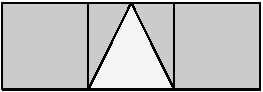
\includegraphics[width=\linewidth]{external/tri-squares.pdf}
\end{image}%
\tcblower
\end{figureptx}%
\item{}Watch the fifth video, \pubtitle{Fractions: Big Ideas} (2:01 minutes), more than once if needed.%
\item{}From the videos in \hyperref[x:task:htlmfs-185-illustrate]{Task~{\xreffont\ref{x:exercise:main-prob-four}}.{\xreffont\ref{x:task:htlmfs-185-illustrate}}} and \hyperref[x:task:htlmfs-solve-again]{Task~{\xreffont\ref{x:exercise:main-prob-four}}.{\xreffont\ref{x:task:htlmfs-solve-again}}}, what big ideas about fractions will help you make sense of them? List at least two.%
\item{}Watch the sixth video in Lesson 5, \pubtitle{Ideas vs. Memorization} (0:53 minutes).%
\begin{enumerate}[font=\bfseries,label=(\roman*),ref=\theenumi.\roman*]
\item{}Think about the mathematical content in our class. What big ideas have you learned so far? What makes them big ideas?%
\item{}What important strategies have you learned? How might these strategies help you in your future mathematics learning?%
\end{enumerate}
\item{}What has surprised you about your learning of mathematics?%
\item{}What additional mathematics would you like to learn?%
\end{enumerate}
\end{inlineexercise}%
\begin{inlineexercise}{}{x:exercise:main-prob-eight}%
Think about your work with mathematics in and out of class so far this semester.%
\begin{enumerate}[font=\bfseries,label=(\alph*),ref=\alph*]
\item{}As you work through activities and problems in and out of class, what messages are you giving yourself? Have you been persistent? Have you told yourself you can do this?%
\item{}The problems we work on in class and for homework often require persistence. What do you do when you struggle with a problem?%
\item{}Have any of your messages to self been negative? If so, based on the videos from \pubtitle{How to Learn Mathematics for Students}, what messages help you grow your brain?%
\end{enumerate}
\end{inlineexercise}%
\begin{inlineexercise}{}{x:exercise:main-prob-nine}%
Answer the following questions. Be specific. Provide examples.%
\begin{enumerate}[font=\bfseries,label=(\alph*),ref=\alph*]
\item{}Why is it important to your mathematical learning to talk about math with others, to make connections, and to use reasoning?%
\item{}How might you use these ways of learning to help you in other subjects?%
\item{}How might you use these ways of learning to help you in your daily life?%
\end{enumerate}
\end{inlineexercise}%
\begin{inlineexercise}{}{x:exercise:main-prob-ten}%
Think about your views of your ability to learn math.%
\begin{enumerate}[font=\bfseries,label=(\alph*),ref=\alph*]
\item{}Have any of your views about your ability to learn math changed this semester? Explain.%
\item{}Watch Video 9 in Lesson 6, \pubtitle{Summary and Reflections} (2:01 minutes). What ideas from \pubtitle{How to Learn Math for Students} stand out for you.%
\item{}Take the survey immediately following Video 9. List the top 5 ideas from the course that stand out for you.%
\item{}Write a reflection, at least 2 paragraphs long, about what you have learned about your ability to learn mathematics.%
\end{enumerate}
\end{inlineexercise}%
\begin{inlineexercise}{}{x:exercise:main-prob-eleven}%
Earn a certificate for completing the Stanford course, How to Learn Math for Students. You may earn privileges as designated by your professor for completing the course and turning in a printed copy of the certificate of completion.%
\end{inlineexercise}%
\end{paragraphs}%
\end{subsectionptx}
%
%
\typeout{************************************************}
\typeout{Subsection 1.1.2 Good Questions to Ask Yourself}
\typeout{************************************************}
%
\begin{subsectionptx}{Good Questions to Ask Yourself}{}{Good Questions to Ask Yourself}{}{}{x:subsection:subsec-good-questions}
When working on mathematics problems, you are in good company if you find that you are often or occasionally stuck. There is always hope. The questions that follow have been used many times to help students find a way out of a temporary dilemma when solving a problem. First, try to identify what's causing your dilemma.%
\par
Do you understand what the problem is asking? If not, you are probably stuck at Stage 1.%
\par
Do you understand the problem but don't know what to do now? You are likely stuck at Stage 2.%
\par
Have you started to solve the problem and gathered some information but don't know what to do with what you've found? You might be stuck at Stage 3.%
\par
Have you finished the problem? Stage 4 questions can help you organize what you've learned through solving the problem into what you already know and help you move new learnings into your long-term memory.%
\par
Goldin (1998) suggests a hierarchy of four stages of questioning to guide yourself or a peer to solve a problem:%
\end{subsectionptx}
%
%
\typeout{************************************************}
\typeout{Subsection 1.1.3 Four Stages of Questioning}
\typeout{************************************************}
%
\begin{subsectionptx}{Four Stages of Questioning}{}{Four Stages of Questioning}{}{}{x:subsection:subsec-qstages}
\begin{paragraphs}{Stage 1: Understanding the Problem.}{x:paragraphs:stageone_questioning}%
Read the problem and take time to make some initial progress on it. Ask yourself:%
\par
%
\begin{itemize}[label=\textbullet]
\item{}What is the problem asking me to do? Write down ideas in your own words.%
\item{}What do I know?%
\item{}What am I trying to find?%
\end{itemize}
%
\end{paragraphs}%
\begin{paragraphs}{Stage 2: Devising a Plan.}{x:paragraphs:stagetwo_questioning}%
If you understand the problem and have trouble starting to solve it, think about general problem-solving strategies that might help. Ask yourself:%
\par
%
\begin{itemize}[label=\textbullet]
\item{}Would drawing a picture help?%
\item{}Would a table of values help to solve this problem?%
\item{}Would any materials help to model the problem? (Get the materials and use them.)%
\item{}Is there a similar problem I've done before that might help me get started?%
\item{}What do I know must happen in the problem?%
\item{}What do I know cannot happen in the problem?%
\end{itemize}
%
\end{paragraphs}%
\begin{paragraphs}{Stage 3: Carrying Out the Plan.}{x:paragraphs:stagethree_questioning}%
If you get stuck once you are partway through solving the problem, think about more specific problem-solving strategies. Ask yourself:%
\par
%
\begin{itemize}[label=\textbullet]
\item{}What patterns do I see in the table of values or drawings?%
\item{}What rule can be used to describe the relationship in the table of values I created?%
\item{}What information does the graph give me?%
\end{itemize}
%
\end{paragraphs}%
\begin{paragraphs}{Stage Four: Looking Back.}{x:paragraphs:stagefour_questioning}%
Once you solve a problem, think back about what you did. Think about your thinking by asking yourself:%
\par
%
\begin{itemize}[label=\textbullet]
\item{}How do I know my solution is correct? How can I convince someone else?%
\item{}How did I think about the problem?%
\item{}Can I solve the problem in another way?%
\item{}How does this problem connect with other problems I have solved?%
\end{itemize}
%
\par
Your goal is to help yourself explain the problem and its solution. This stage helps you mentally file your thoughts about the problem in a category with other similar problems, organizing your new learning into your long-term memory.%
\par
Table based on Goldin, Gerald A. ``Observing Mathematical Problem Solving through Task-Based Interviews''. In Anne R. Teppo (Ed.), \pubtitle{Qualitative Research Methods in Mathematics Education} (pp. 40-62). Reston, VA: National Council of Teachers of Mathematics, 1998.%
\end{paragraphs}%
\end{subsectionptx}
%
%
\typeout{************************************************}
\typeout{Subsection 1.1.4 Other Helpful Practices}
\typeout{************************************************}
%
\begin{subsectionptx}{Other Helpful Practices}{}{Other Helpful Practices}{}{}{x:subsection:subsec-practices}
To best learn mathematics, you will find that each of the following strategies are helpful if you make them a habit:%
\begin{paragraphs}{Read carefully.}{g:paragraphs:idp1871473912}%
It might be necessary to read problems or narration several times in order to understand more fully what each intends. Students who do not read carefully always make mistakes that can be remedied by rereading more carefully.%
\end{paragraphs}%
\begin{paragraphs}{Organize your work.}{g:paragraphs:idp1871476216}%
Use tables and graphs to help you make sense of information you find when solving a problem. Don't underestimate the power of trying a few numbers to see what happens. Always keep track of what you try. Do not erase or throw away attempts that don't work. Save them and compare them to an approach that did finally work. Ask yourself these questions: What was I thinking initially? What do I now know? Was I far off at the beginning? If not, what was I thinking that could have led me to a correct solution? If so, what was I thinking that was helpful? What was getting in the way of my understanding?%
\end{paragraphs}%
\begin{paragraphs}{Check your solutions to see that they make sense.}{g:paragraphs:idp1871475704}%
If a context is given, translate your solutions into the context. Check to make sure any numbers you're getting from equations, tables, or graphs make sense in the context. Make sure graphs, tables, and equations give corresponding information.%
\end{paragraphs}%
\begin{paragraphs}{Never give up!}{g:paragraphs:idp1871476856}%
It's OK to take a break from a problem that's frustrating you. Return to it after you've had a chance to relieve your frustration. You can learn mathematics. You can solve any problem facing you, \emph{as long as you never give up!}%
\end{paragraphs}%
\begin{paragraphs}{Study at least a little \emph{most days}.}{g:paragraphs:idp1871472632}%
After each class, take 15 minutes to write down what you learned. Be specific. For example, don't state, ``I learned about linear functions.'' Instead, state specifically what you learned, ``I learned that the slope of a linear function when shown in a graph is the value of \(m\) in the equation, \(y = mx + b\). This makes sense, because slope is how much \(y\) changes when \(x\) changes by 1 so in a graph, the \(y\)-value of a linear function changes by \(m\) every time \(x\) changes by 1.''%
\end{paragraphs}%
\begin{paragraphs}{Do your assigned homework.}{g:paragraphs:idp1871481336}%
Homework provides you the opportunity to grow your brain outside of class. It also prepares you to think about problems that build on your homework when you are in class. Making mistakes is an important part of learning, so grading your early thoughts about a topic is counterproductive. \emph{Doing} homework, however, grows your brain, allows you to get more out of the work you're doing in class, and helps you prepare for your future with technical information. Not doing homework is detrimental to you, and to your current and future work!%
\end{paragraphs}%
\begin{paragraphs}{Commit to your education.}{g:paragraphs:idp1871482872}%
Participate fully in your group and class and make every effort to complete your homework so that you're prepared to participate with your group.%
\end{paragraphs}%
\end{subsectionptx}
%
%
\typeout{************************************************}
\typeout{Subsection 1.1.5 Mathematical Practices}
\typeout{************************************************}
%
\begin{subsectionptx}{Mathematical Practices}{}{Mathematical Practices}{}{}{x:subsection:subsec-math-practices}
Several practices have been identified that can help you make sense of problems that arise in your daily work and in technical situations. Which practices do you use to learn mathematics and other content fields? When you work on mathematics, use this page to help you choose strategies that might help you learn. Revisit this page often, especially when you get stuck, for suggestions of other strategies you might try as you're trying to solve problems. \href{http://www.corestandards.org/Math/Practice/}{Resource.}\footnote{\nolinkurl{corestandards.org/Math/Practice/}\label{g:fn:idp1871477880}}%
\begin{figureptx}{A diagram of the mathematical practices.}{x:figure:fig-math-practices}{}%
\begin{image}{0}{1}{0}%
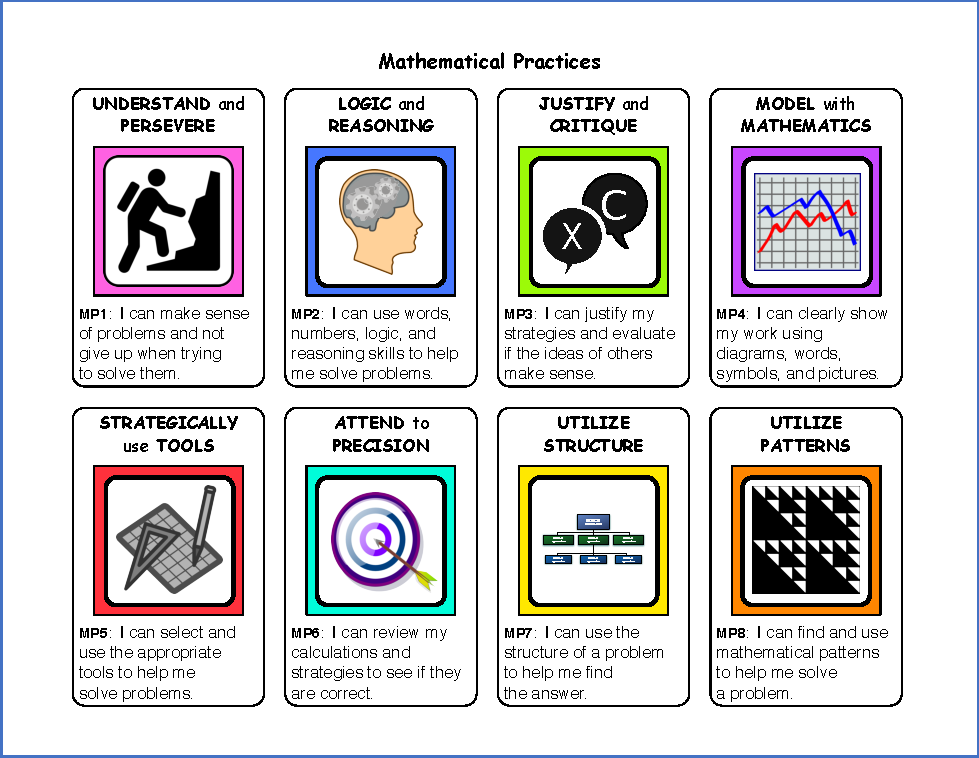
\includegraphics[width=\linewidth]{external/math-practices.pdf}
\end{image}%
\tcblower
\end{figureptx}%
\end{subsectionptx}
%
%
\typeout{************************************************}
\typeout{Homework 1.1.6 Homework}
\typeout{************************************************}
%
\begin{exercises-subsection}{Homework}{}{Homework}{}{}{x:exercises:exercises_sec-one}
Complete the following homework before the next class period:%
\begin{divisionexercise}{1}{}{}{g:exercise:idp1871481976}%
Go back to \hyperlink{x:paragraphs:htlmfs-directions}{How To Learn Math For Students Directions}. Complete \hyperref[x:exercise:main-prob-one]{How to Learn Math for Students Exercise~{\xreffont\ref{x:exercise:main-prob-one}}}. You will hand in your written reflections for problem 1 in class.%
\end{divisionexercise}%
\begin{divisionexercise}{2}{}{}{g:exercise:idp1871486200}%
Read the sections above, \hyperref[x:subsection:subsec-good-questions]{Good Questions to Ask Yourself}, \hyperref[x:subsection:subsec-practices]{Other Helpful Practices}, and \hyperref[x:subsection:subsec-math-practices]{Mathematical Practices}. Remember these sections as you work your way through the activities in this course. Refer to each section as needed. Write a one sentence description of each section to help you remember when to consult each of these sections.%
\end{divisionexercise}%
\end{exercises-subsection}
\end{sectionptx}
%
%
\typeout{************************************************}
\typeout{Section 1.2 Thinking Together and Mathematical Mindset}
\typeout{************************************************}
%
\begin{sectionptx}{Thinking Together and Mathematical Mindset}{}{Thinking Together and Mathematical Mindset}{}{}{x:section:S_mathmindset}
%
%
\typeout{************************************************}
\typeout{Subsection 1.2.1 Video: Mindset}
\typeout{************************************************}
%
\begin{subsectionptx}{Video: Mindset}{}{Video: Mindset}{}{}{x:subsection:subsec-mindset-video}
The message of ``Mindset'' is that everyone can learn mathematics. The video includes important brain and mindset evidence to support this message. Watch the video. Write a brief reflection, then discuss the video in small groups. This video is from \href{https://www.youcubed.org/resources/mindset-video/}{Week 1 of Inspirational Math, Day 1}\footnote{\nolinkurl{youcubed.org/resources/mindset-video/}\label{g:fn:idp1871490680}}.%
\begin{figureptx}{``Mindset'' Video.}{x:figure:vid-mindsets}{}%
\centering
\setlength{\qrsize}{9em}
\setlength{\previewwidth}{\linewidth}
\addtolength{\previewwidth}{-\qrsize}
\begin{tcbraster}[raster columns=2, raster column skip=1pt, raster halign=center, raster force size=false, raster left skip=0pt, raster right skip=0pt]%
\begin{tcolorbox}[previewstyle, width=\previewwidth]%
\mono{No preview image available}%
\end{tcolorbox}%
\begin{tcolorbox}[qrstyle]%
{\hypersetup{urlcolor=black}\qrcode[height=\qrsize]{https://vimeo.com/126645788}}%
\end{tcolorbox}%
\begin{tcolorbox}[captionstyle]%
\small \mono{vimeo.com/126645788}\end{tcolorbox}%
\end{tcbraster}%
\tcblower
\end{figureptx}%
\end{subsectionptx}
%
%
\typeout{************************************************}
\typeout{Student Page 1.2.2 Good Group Work (Also from Week 1 of Inspirational Math)}
\typeout{************************************************}
%
\newgeometry{left=1.2in, right=1.2in, top=1in, bottom=1in}
\begin{worksheet-subsection}{Good Group Work (Also from Week 1 of Inspirational Math)}{}{Good Group Work (Also from Week 1 of Inspirational Math)}{}{}{x:worksheet:act-group-work}
\begin{introduction}{}%
\begin{quote}%
If you want to go fast, go alone, if you want to go far, go together.%
\nopagebreak\par%
\hfill\textemdash{}{\setlength{\tabcolsep}{0pt}\begin{tabular}[t]{l@{}}
African Proverb
\end{tabular}}\\\par
\end{quote}
Before you work on math together, complete this activity. Use the cooperative learning strategy, \hyperlink{x:paragraphs:mindset-roundtable}{Roundtable}, to generate ideas.%
\end{introduction}%
\begin{paragraphs}{Roundtable.}{x:paragraphs:mindset-roundtable}%
Each team uses a single sheet of paper.%
\par
The team member closest to the classroom door writes down an idea, states it out loud, and passes the paper to the left.%
\par
Other group members may ask for clarification but may not critique the idea.%
\par
Continue until time is called.%
\end{paragraphs}%
\par
This activity will help improve group interactions. Teachers who have tried this activity have been pleased by students' thoughtful responses and found students' thoughts and words helpful in creating a positive and supportive environment. Use \hyperlink{x:paragraphs:mindset-roundtable}{Roundtable} to reflect on things you like people to say or do in a group when you are working together. After you have thought of and written down a few of the ideas, use \hyperlink{x:paragraphs:mindset-roundtable}{Roundtable} to reflect on things you don't like people to say or do when you are working in a group.%
\par
Some important ideas students generally share include: Let everyone share their ideas, share different ways to solve a problem, listen when others speak, don't give away the answer, don't rush through the work, and don't ignore other people's ideas.%
\par
When the class has finished brainstorming, share ideas on a ``What we like'' poster with each group contributing at least one idea. Do the same for a ``What we don't like'' poster. Post the final posters in class as the agreed upon classroom norms; refer back to them throughout the course, as needed. Don't include negative comments such as, ``I don't like waiting for slow people,'' instead discuss the issue.%
\end{worksheet-subsection}
\restoregeometry
%
%
\typeout{************************************************}
\typeout{Student Page 1.2.3 Mindset Survey}
\typeout{************************************************}
%
\newgeometry{left=1.2in, right=1.2in, top=1in, bottom=1in}
\begin{worksheet-subsection}{Mindset Survey}{}{Mindset Survey}{}{}{x:worksheet:act-mindset}
\begin{introduction}{}%
Document your current feelings about how you approach mathematics through the following.%
\end{introduction}%
\begin{divisionexercise}{1}{}{}{x:exercise:mindset-one}%
Look at \hyperref[x:figure:fig-mindsets]{Figure~{\xreffont\ref{x:figure:fig-mindsets}}}. Follow the directions to get a baseline of your attitudes concerning your ability to learn mathematics.%
\begin{figureptx}{A depiction of mathematical mindsets.}{x:figure:fig-mindsets}{}%
\begin{image}{0.25}{0.5}{0.25}%
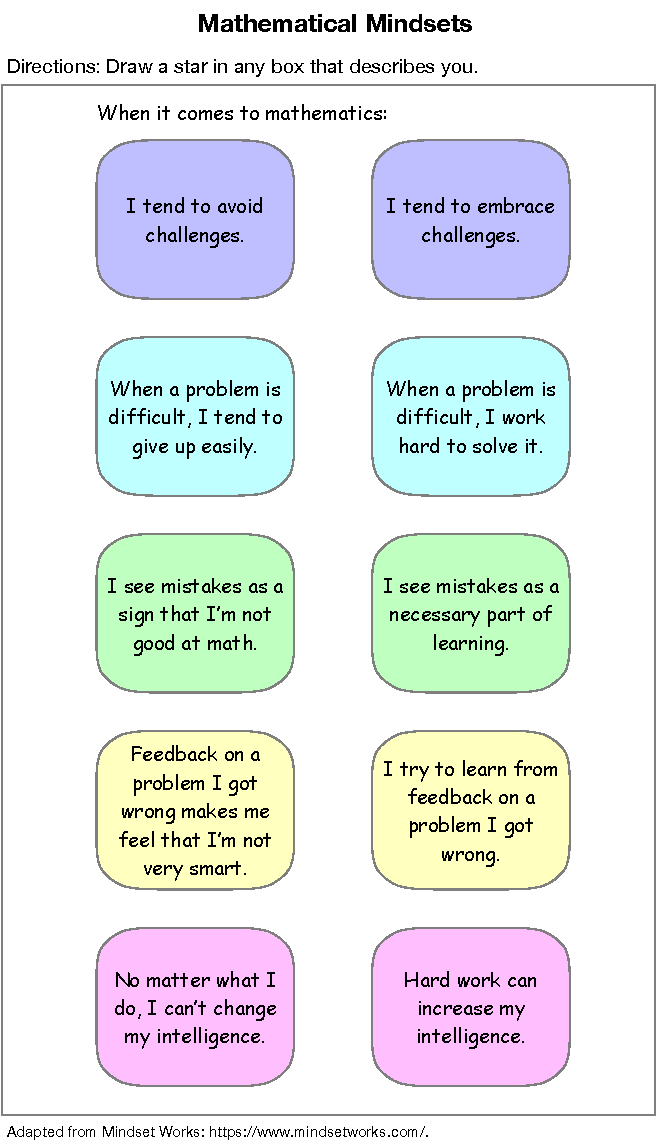
\includegraphics[width=\linewidth]{external/mindsets.pdf}
\end{image}%
\tcblower
\end{figureptx}%
\end{divisionexercise}%
\begin{divisionexercise}{2}{}{}{x:exercise:mindset-two}%
\begin{enumerate}[font=\bfseries,label=(\alph*),ref=\alph*]
\item{}The boxes in the first column of \hyperref[x:figure:fig-mindsets]{Figure~{\xreffont\ref{x:figure:fig-mindsets}}} describe a person with a Fixed Mindset. The boxes in the second column describe a person with a Growth Mindset. At the present time, do you tend to have a Fixed Mindset or a Growth Mindset in terms of learning mathematics? Explain why you think so.%
\item{}Having a Growth Mindset helps you overcome obstacles as you work to learn mathematics. Having a Fixed Mindset, on the other hand, can prevent you from learning mathematics. It is important to work to overcome a Fixed Mindset so that it doesn't hold you back from learning. If you tend to have a Fixed Mindset, what ideas do you have to help you transition from a Fixed to a Growth Mindset?%
\end{enumerate}
\end{divisionexercise}%
\begin{divisionexercise}{3}{}{}{x:exercise:mindset-three}%
\begin{enumerate}[font=\bfseries,label=(\alph*),ref=\alph*]
\item{}Keep your responses to \hyperlink{x:exercise:mindset-one}{Student Page Exercise~{\xreffont 1.2.3.1}} and \hyperlink{x:exercise:mindset-two}{Student Page Exercise~{\xreffont 1.2.3.2}}. Revisit them often. Each time, ask yourself:%
\begin{itemize}[label=\textbullet]
\item{}Have any of my beliefs changed?%
\item{}Do I believe in myself and my ability to learn mathematics?%
\end{itemize}
If the answer to either question is no, ask yourself:%
\begin{itemize}[label=\textbullet]
\item{}What messages am I giving myself that keep me from believing in myself?%
\item{}What messages would be more helpful?%
\end{itemize}
%
\end{enumerate}
\end{divisionexercise}%
\end{worksheet-subsection}
\restoregeometry
\begin{activity}{Making Introductions.}{x:activity:act-introductions}%
In this activity, in turn, you will introduce yourself using alliteration. You will also introduce everyone who was introduced before you. Suppose the first 3 persons are Char, Ben, and Melanie. Char starts by saying: ``I'm Char. I like shopping in Chicago.'' Ben says, ``I'm Ben. I like baseball. This is Char; she likes shopping in Chicago.'' Melanie might say, ``I'm Melanie, I like making meals. This is Ben; he likes baseball. This is Char; she likes shopping in Chicago.'' Introductions continue around the room with successive students introducing everyone who came before them. If there are 30 students or more in class, the first half of the students introduce themselves using this scheme, then the second half does the same starting over with the first person of the second group.%
\par
Once introductions have been made, complete the following:%
\begin{enumerate}[font=\bfseries,label=(\alph*),ref=\alph*]
\item{}Create a table to show the number of introductions made by each of the first 5 people and also the total number of introductions made so far.%
\item{}Look for and share any patterns you see in the table.%
\item{}Determine the total number of introductions that have been made after 10 people, 15 people, and 20 people.%
\item{}Is there a way to find the number of introductions made by the whole class? How? What is the number? How do you know?%
\end{enumerate}
\end{activity}%
%
%
\typeout{************************************************}
\typeout{Homework 1.2.4 Homework}
\typeout{************************************************}
%
\begin{exercises-subsection}{Homework}{}{Homework}{}{}{x:exercises:exercises-12}
\begin{divisionexercise}{1}{}{}{g:exercise:idp1871510264}%
Complete \hyperref[x:exercise:main-prob-two]{How to Learn Math for Students Exercise~{\xreffont\ref{x:exercise:main-prob-two}}}. You will hand in your written reflections for \hyperref[x:exercise:main-prob-two]{How to Learn Math for Students Exercise~{\xreffont\ref{x:exercise:main-prob-two}}} in class.%
\end{divisionexercise}%
\begin{divisionexercise}{2}{}{}{g:exercise:idp1871517688}%
Answer the bulleted questions in \hyperref[x:activity:act-introductions]{Making Introductions}. Be ready to share your responses with the class.%
\end{divisionexercise}%
\begin{divisionexercise}{3}{}{}{g:exercise:idp1871511928}%
Take the \href{https://www.mindsetworks.com/assess/}{Mindset Survey online}\footnotemark{}. Read the recommendations provided once you take the survey. Print out a copy of these recommendations or store the results on your computer. Consult the results any time you feel frustrated with your work in this course.%
\end{divisionexercise}%
\footnotetext[4]{\nolinkurl{mindsetworks.com/assess/}\label{g:fn:idp1871510136}}%
\end{exercises-subsection}
\end{sectionptx}
%
%
\typeout{************************************************}
\typeout{Section 1.3 Connecting Mathematics Through Representations}
\typeout{************************************************}
%
\begin{sectionptx}{Connecting Mathematics Through Representations}{}{Connecting Mathematics Through Representations}{}{}{x:section:S_connectmath}
\begin{introduction}{}%
Much of mathematics involves the study of patterns. Making sense of patterns happens through interconnections among representations. In \hyperref[x:section:S_connectmath]{Section~{\xreffont\ref{x:section:S_connectmath}}}, we begin with a visual growing pattern of dots, connect it with a pattern of numbers, and graphs that model different interpretations of the pattern. Finally, we connect the pattern to a familiar context. All of these representations help us makes sense of one or more aspects of how the pattern is growing, how to analyze it, and how to generalize it.%
\end{introduction}%
%
%
\typeout{************************************************}
\typeout{Subsection 1.3.1 Video: Brain Crossing}
\typeout{************************************************}
%
\begin{subsectionptx}{Video: Brain Crossing}{}{Video: Brain Crossing}{}{}{x:subsection:subsec-brain-crossing}
The video shares some important new research on the power of engaging with numbers and symbols visually, which involves brain crossing. Your brain is capable of learning through visual cues, especially if you connect them to other modes of learning. The video explains that it is helpful for all students to think visually about mathematics. ``Brain Crossing'' is found in \href{https://www.youcubed.org/resources/brain-crossing-video/}{Week 1 of Inspirational Math, Day 2}\footnote{\nolinkurl{youcubed.org/resources/brain-crossing-video/}\label{g:fn:idp1871519224}}.%
\end{subsectionptx}
%
%
\typeout{************************************************}
\typeout{Subsection 1.3.2 Pattern Talk: Dot Pattern}
\typeout{************************************************}
%
\begin{subsectionptx}{Pattern Talk: Dot Pattern}{}{Pattern Talk: Dot Pattern}{}{}{x:subsection:SS_dot_pattern}
Consider the dot arrangement in \hyperref[x:figure:fig-dots]{Figure~{\xreffont\ref{x:figure:fig-dots}}}. How many dots are in the arrangement? Explain how you counted the dots. Share as many ways of counting the dots as possible.%
\begin{figureptx}{}{x:figure:fig-dots}{}%
\begin{image}{0.4}{0.2}{0.4}%

\includegraphics[width=\linewidth]{external/tri-dots.pdf}
\end{image}%
\tcblower
\end{figureptx}%
Show the different ways you counted the dots by drawing on each figure in \hyperref[x:figure:fig-five-dots]{Figure~{\xreffont\ref{x:figure:fig-five-dots}}}.%
\begin{figureptx}{}{x:figure:fig-five-dots}{}%
\begin{sidebyside}{5}{0.015}{0.015}{0.03}%
\begin{sbspanel}{0.17}%

\includegraphics[width=\linewidth]{external/tri-dots.pdf}
\end{sbspanel}%
\begin{sbspanel}{0.17}%

\includegraphics[width=\linewidth]{external/tri-dots.pdf}
\end{sbspanel}%
\begin{sbspanel}{0.17}%

\includegraphics[width=\linewidth]{external/tri-dots.pdf}
\end{sbspanel}%
\begin{sbspanel}{0.17}%

\includegraphics[width=\linewidth]{external/tri-dots.pdf}
\end{sbspanel}%
\begin{sbspanel}{0.17}%

\includegraphics[width=\linewidth]{external/tri-dots.pdf}
\end{sbspanel}%
\end{sidebyside}%
\tcblower
\end{figureptx}%
Mathematics is a creative endeavor. There is always more than one way to solve a problem. If you get stuck, try to find another route!%
\end{subsectionptx}
%
%
\typeout{************************************************}
\typeout{Student Page 1.3.3 Growing Pattern of Dots}
\typeout{************************************************}
%
\newgeometry{left=1.2in, right=1.2in, top=1in, bottom=1in}
\begin{worksheet-subsection}{Growing Pattern of Dots}{}{Growing Pattern of Dots}{}{}{x:worksheet:act-growing-dots}
\begin{introduction}{}%
Now consider a pattern related to \hyperref[x:figure:fig-five-dots]{Figure~{\xreffont\ref{x:figure:fig-five-dots}}}. See the student page, \hyperref[x:worksheet:act-growing-dots]{Growing Pattern of Dots}.%
\par
Spend at least 5 minutes thinking about the problem on your own.%
\par
When everyone in your group is ready, share your solutions to \hyperref[x:worksheet:act-growing-dots]{Growing Pattern of Dots} with each other. Try to resolve any differences you have in your understandings. If you and your group members are still uncertain about something after your discussion, write a question or two to ask the full class.%
\par
Consider the pattern of dot arrangements in \hyperref[x:figure:fig-growing-dots]{Figure~{\xreffont\ref{x:figure:fig-growing-dots}}}.%
\begin{figureptx}{}{x:figure:fig-growing-dots}{}%
\begin{image}{0}{1}{0}%
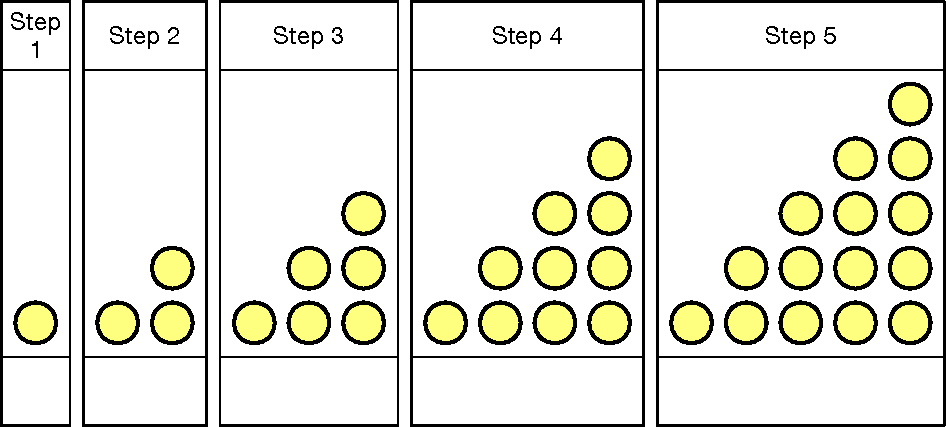
\includegraphics[width=\linewidth]{external/growing-dots.pdf}
\end{image}%
\tcblower
\end{figureptx}%
\end{introduction}%
\begin{divisionexercise}{1}{}{}{g:exercise:idp1871532408}%
How are these dots related to the dots you counted in the \hyperref[x:subsection:SS_dot_pattern]{Pattern Talk: Dot Pattern}?%
\end{divisionexercise}%
\begin{divisionexercise}{2}{}{}{g:exercise:idp1871541752}%
\begin{enumerate}[font=\bfseries,label=(\alph*),ref=\alph*]
\item{}How is each arrangement of dots related to the arrangement in the step before it?%
\item{}How is each arrangement of dots related to the arrangement in the step after it?%
\end{enumerate}
\end{divisionexercise}%
\begin{divisionexercise}{3}{}{}{g:exercise:idp1871538680}%
\begin{enumerate}[font=\bfseries,label=(\alph*),ref=\alph*]
\item{}Is this pattern of dots related to \hyperref[x:activity:act-introductions]{Making Introductions}? How?%
\end{enumerate}
\end{divisionexercise}%
\begin{divisionexercise}{4}{}{}{x:exercise:exer-grow-dots-describe-strat}%
Consider the strategies you and classmates used to count the arrangement of dots in the \hyperref[x:subsection:SS_dot_pattern]{Pattern Talk: Dot Pattern}. Choose one strategy that works to count the dots in each of the arrangements.%
\begin{enumerate}[font=\bfseries,label=(\alph*),ref=\alph*]
\item{}Describe the strategy.%
\item{}Use the strategy, show how you used it for each step, and record the number of dots in each arrangement in the bottom row of \hyperref[x:figure:fig-growing-dots]{Figure~{\xreffont\ref{x:figure:fig-growing-dots}}}.%
\end{enumerate}
\end{divisionexercise}%
\begin{divisionexercise}{5}{}{}{x:exercise:exer-grow-dots-step10}%
How many dots will there be in step 10? How do you know?%
\end{divisionexercise}%
\begin{conclusion}{}%
Share your responses with the full class:%
\par
Which strategy did you use to count the dots in each of these arrangements? Show how you used the same strategy to count the dots in \hyperlink{x:exercise:exer-grow-dots-describe-strat}{Student Page Exercise~{\xreffont 1.3.3.4}} and \hyperlink{x:exercise:exer-grow-dots-step10}{Student Page Exercise~{\xreffont 1.3.3.5}}.%
\par
Does the strategy you used to count each dot arrangement help you determine the number of introductions that were made in our class? Explain.%
\par
What questions do you still have? (Resolve these as a class.)%
\end{conclusion}%
\end{worksheet-subsection}
\restoregeometry
%
%
\typeout{************************************************}
\typeout{Student Page 1.3.4 Graphing a Growing Pattern of Dots}
\typeout{************************************************}
%
\newgeometry{left=1.2in, right=1.2in, top=1in, bottom=1in}
\begin{worksheet-subsection}{Graphing a Growing Pattern of Dots}{}{Graphing a Growing Pattern of Dots}{}{}{x:worksheet:act-graphing-dots}
\begin{divisionexercise}{1}{}{}{g:exercise:idp1871549688}%
Consider the data table you created for \hyperref[x:worksheet:act-growing-dots]{Growing Pattern of Dots}. The data is plotted in the following graphs. For each graph, determine: \begin{sidebyside}{4}{0}{0}{0}%
\begin{sbspanel}{0.25}%
\begin{figureptx}{}{x:figure:fig-graphing-dots1}{}%
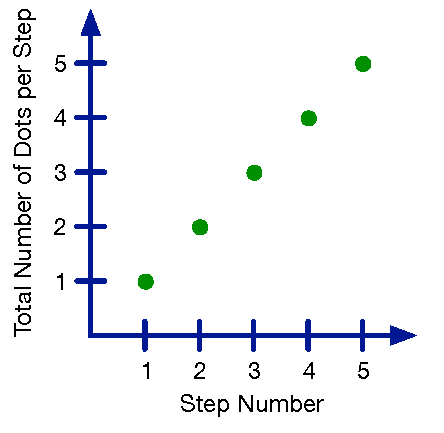
\includegraphics[width=\linewidth]{external/graphing-dots1.pdf}
\tcblower
\end{figureptx}%
\end{sbspanel}%
\begin{sbspanel}{0.25}%
\begin{figureptx}{}{x:figure:fig-graphing-dots2}{}%
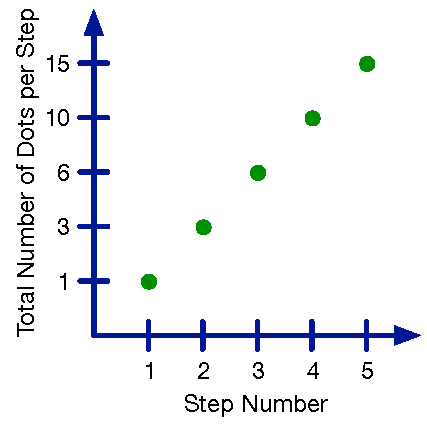
\includegraphics[width=\linewidth]{external/graphing-dots2.pdf}
\tcblower
\end{figureptx}%
\end{sbspanel}%
\begin{sbspanel}{0.25}%
\begin{figureptx}{}{x:figure:fig-graphing-dots3}{}%
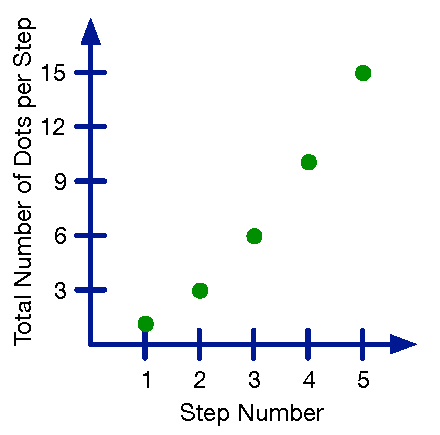
\includegraphics[width=\linewidth]{external/graphing-dots3.pdf}
\tcblower
\end{figureptx}%
\end{sbspanel}%
\begin{sbspanel}{0.25}%
\begin{figureptx}{}{x:figure:fig-graphing-dots4}{}%
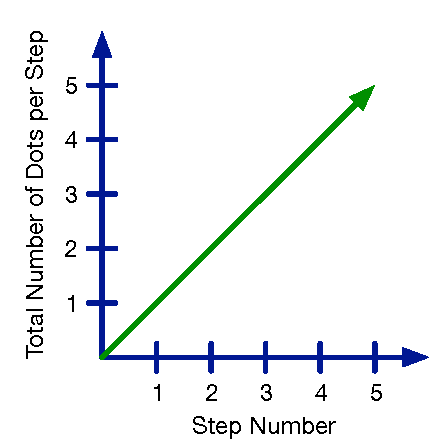
\includegraphics[width=\linewidth]{external/graphing-dots4.pdf}
\tcblower
\end{figureptx}%
\end{sbspanel}%
\end{sidebyside}%
%
\begin{enumerate}[font=\bfseries,label=(\alph*),ref=\alph*]
\item{}Is the graph a correct representation of the data?%
\item{}Why or why not?%
\end{enumerate}
\end{divisionexercise}%
\begin{divisionexercise}{2}{}{}{g:exercise:idp1871547256}%
What are some important characteristics of an accurate graph? List of at least 5 items.%
\end{divisionexercise}%
\begin{conclusion}{}%
This collection of activities \textendash{} \hyperref[x:activity:act-introductions]{Making Introductions}, \hyperref[x:subsection:SS_dot_pattern]{Pattern Talk: Dot Pattern}, \hyperref[x:worksheet:act-growing-dots]{Growing Pattern of Dots}, and \hyperref[x:worksheet:act-graphing-dots]{Graphing a Growing Pattern of Dots} \textendash{} shows how seemingly unrelated contexts and representations can have the same underlying mathematical structure. We see this a lot in mathematics. Making these connections requires Brain Crossing (recall the video you watched today). Remember that Brain Crossing helps you with recall and grows your brain!%
\par
When you work on a new problem, try to connect the work you're doing to problems you've worked on in the past. Connecting related mathematics problems helps reduce your reliance on memorized procedures. It also helps move your working (short-term) memory into long-term memory so that it can be retrieved to help you make sense of new problems and concepts.%
\end{conclusion}%
\end{worksheet-subsection}
\restoregeometry
%
%
\typeout{************************************************}
\typeout{Homework 1.3.5 Homework}
\typeout{************************************************}
%
\begin{exercises-subsection}{Homework}{}{Homework}{}{}{x:exercises:exercises13}
\begin{introduction}{}%
Complete the following homework before the next class period:%
\end{introduction}%
\begin{divisionexercise}{1}{}{}{g:exercise:idp1871551864}%
Go back to \hyperlink{x:paragraphs:htlmfs-directions}{How To Learn Math For Students Directions} from \hyperref[x:section:S_learnmath]{Section~{\xreffont\ref{x:section:S_learnmath}}}. Complete \hyperref[x:exercise:main-prob-three]{How to Learn Math for Students Exercise~{\xreffont\ref{x:exercise:main-prob-three}}}. You will hand in your written reflections for \hyperref[x:exercise:main-prob-three]{How to Learn Math for Students Exercise~{\xreffont\ref{x:exercise:main-prob-three}}} in class.%
\end{divisionexercise}%
\begin{divisionexercise}{2}{}{}{g:exercise:idp1871555704}%
Revisit each of teh related activites \hyperref[x:activity:act-introductions]{Making Introductions}, \hyperref[x:subsection:SS_dot_pattern]{Pattern Talk: Dot Pattern}, \hyperref[x:worksheet:act-growing-dots]{Growing Pattern of Dots}, and \hyperref[x:worksheet:act-graphing-dots]{Graphing a Growing Pattern of Dots}. Write a paragraph or two that shows your understanding of how each of these activities is related.%
\end{divisionexercise}%
\begin{divisionexercise}{3}{}{}{g:exercise:idp1871558904}%
Critique the graph below. If the graph is accurate, say how you know. If the graph is incorrect, indicate all the ways it needs to be fixed, label the axes correctly, and redraw the graph. \begin{sidebyside}{2}{0}{0}{0}%
\begin{sbspanel}{0.5}%
\resizebox{\ifdim\width > \linewidth\linewidth\else\width\fi}{!}{%
{\centering%
{\tabularfont%
\begin{tabular}{Acc}\hrulethin
\multicolumn{1}{AcA}{\textbf{\(x\)}}&\multicolumn{1}{cA}{\textbf{\(y\)}}\tabularnewline\hrulethin
\multicolumn{1}{AcA}{1}&\multicolumn{1}{cA}{1.2}\tabularnewline\hrulethin
\multicolumn{1}{AcA}{10}&\multicolumn{1}{cA}{24}\tabularnewline\hrulethin
\multicolumn{1}{AcA}{15}&\multicolumn{1}{cA}{36}\tabularnewline\hrulethin
\multicolumn{1}{AcA}{50}&\multicolumn{1}{cA}{60}\tabularnewline\hrulethin
\end{tabular}
}%
\par}
}%
\end{sbspanel}%
\begin{sbspanel}{0.5}%
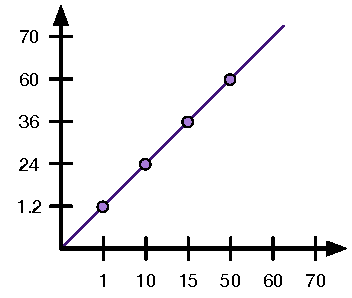
\includegraphics[width=\linewidth]{external/critique-graph.pdf}
\end{sbspanel}%
\end{sidebyside}%
%
\end{divisionexercise}%
\begin{divisionexercise}{4}{}{}{g:exercise:idp1871563256}%
The same growing number pattern is shown twice in \hyperref[x:figure:fig-counting-dots]{Figure~{\xreffont\ref{x:figure:fig-counting-dots}}} Illustrate on the figures and explain in words how you are counting each set of dots in the pattern.%
\begin{figureptx}{}{x:figure:fig-counting-dots}{}%
\begin{image}{0.15}{0.7}{0.15}%
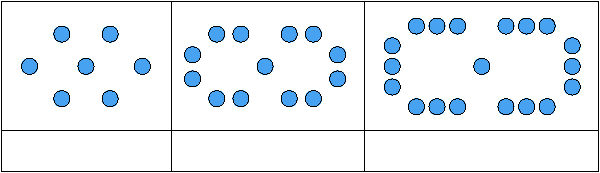
\includegraphics[width=\linewidth]{external/counting-dots.pdf}
\end{image}%
\begin{image}{0.15}{0.7}{0.15}%
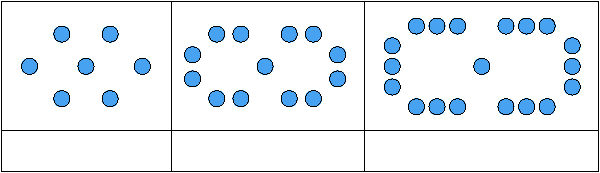
\includegraphics[width=\linewidth]{external/counting-dots.pdf}
\end{image}%
\tcblower
\end{figureptx}%
\begin{enumerate}[font=\bfseries,label=(\alph*),ref=\alph*]
\item\label{x:task:countingdotsa}Count the number of dots in the first set of \hyperref[x:figure:fig-counting-dots]{Figure~{\xreffont\ref{x:figure:fig-counting-dots}}} using the same method to count all three arrangements of dots.%
\item{}Count the number of dots in the second set of \hyperref[x:figure:fig-counting-dots]{Figure~{\xreffont\ref{x:figure:fig-counting-dots}}} using a different method from the method you used in \hyperref[x:task:countingdotsa]{Task~{\xreffont 1.3.5.4}.{\xreffont\ref{x:task:countingdotsa}}}. Use this second method to count all three arrangements of dots.%
\item{}What number of dots will be in the next figure? How do you know? Include a drawing of the figure in your explanation.%
\end{enumerate}
\end{divisionexercise}%
\begin{divisionexercise}{5}{}{}{g:exercise:idp1871567864}%
Consider each of the stories and expressions on the student page, \hyperref[x:worksheet:act-interpret-express]{Interpreting Expressions}. What do you notice about the expressions? Which ones name the same number? Why?%
\end{divisionexercise}%
\begin{divisionexercise}{6}{}{}{g:exercise:idp1871570680}%
Read the introduction to \hyperref[x:section:S_orderofop]{Section~{\xreffont\ref{x:section:S_orderofop}}}. In writing, answer each question in the reading.%
\end{divisionexercise}%
\end{exercises-subsection}
%
%
\typeout{************************************************}
\typeout{Student Page 1.3.6 Interpreting Expressions}
\typeout{************************************************}
%
\newgeometry{left=1.2in, right=1.2in, top=1in, bottom=1in}
\begin{worksheet-subsection}{Interpreting Expressions}{}{Interpreting Expressions}{}{}{x:worksheet:act-interpret-express}
\begin{introduction}{}%
\begin{center}%
{\tabularfont%
\begin{tabular}{Alc}\hrulethin
\multicolumn{1}{AlB}{\tablecelllines{l}{m}
{I am making apple pie and apple turnovers.\\
One recipe calls for 2 apples. The other\\
recipe calls for 3 apples. I'm making 5\\
recipes of each dessert. How many apples\\
do I need?}
}&\multicolumn{1}{cA}{\(2 + ( 3 \times 5 )\)}\tabularnewline\hrulethin
\multicolumn{1}{AlB}{\tablecelllines{l}{m}
{I have 2 one-dollar bills and 3 five-dollar\\
bills. How much money do I have?}
}&\multicolumn{1}{cA}{\(( 2 + 3 ) \times 5\)}\tabularnewline\hrulethin
\multicolumn{1}{AlB}{\tablecelllines{l}{m}
{Mom lets me keep any money I find when I\\
clean the house. She also quadruples any\\
money I find to pay me for my work. I\\
found \textdollar{}2 in the couch and \textdollar{}3 in my dad's\\
jacket. How much money will I have after\\
Mom pays me?}
}&\multicolumn{1}{cA}{\(2 + 3 \times 5\)}\tabularnewline\hrulethin
\multicolumn{1}{AlB}{\tablecelllines{l}{m}
{I need 2 cups of almond flour to make a\\
batch of pancakes and 3 cups of almond\\
flour to make a cake. I'm going to make 5\\
cakes and 1 batch of pancakes. How much\\
flour will I need?}
}&\multicolumn{1}{cA}{\(2 + 3 + ( 2 + 3 ) \times 4\)}\tabularnewline\hrulethin
\end{tabular}
}%
\end{center}%
\end{introduction}%
\begin{divisionexercise}{1}{}{}{g:exercise:idp1871579640}%
Decide which numeric expression best fits each story. Be ready to defend your choices.%
\end{divisionexercise}%
\begin{divisionexercise}{2}{}{}{g:exercise:idp1871589496}%
Decide which numeric expressions, if any, represent the same value.%
\end{divisionexercise}%
\end{worksheet-subsection}
\restoregeometry
\end{sectionptx}
%
%
\typeout{************************************************}
\typeout{Section 1.4 Flexibility with Numbers and Order of Operations}
\typeout{************************************************}
%
\begin{sectionptx}{Flexibility with Numbers and Order of Operations}{}{Flexibility with Numbers and Order of Operations}{}{}{x:section:S_orderofop}
\begin{introduction}{}%
In \hyperref[x:section:S_orderofop]{Section~{\xreffont\ref{x:section:S_orderofop}}}, you will use your creativity and play with mathematical operations using the Order of Operations. The Order of Operations is an agreed upon order in which operations must be completed when simplifying a numeric or an algebraic expression. When presented as a list of rules, the Order of Operations can seem arbitrary. However, there are mathematical reasons underlying the order in which operations are completed.%
\end{introduction}%
%
%
\typeout{************************************************}
\typeout{Subsection 1.4.1 The Order of Operations}
\typeout{************************************************}
%
\begin{subsectionptx}{The Order of Operations}{}{The Order of Operations}{}{}{g:subsection:idp1871588344}
The Order of Operations follows the historical introduction of operations. Addition happened first. Subtraction is the operation that undoes addition. Multiplication naturally occurred as people needed to determine multiple sums of the same number; multiplication is repeated addition. The operation that undoes multiplication is division; division can also be thought of as repeated subtraction. Exponentiation occurred even later signifying repeated multiplication. Taking a whole number root, the inverse operation of raising a number to the same whole number exponent, can also be thought of as repeated division. When you encounter an expression to be simplified, consider the historical introduction of arithmetic operations and perform the most complex operation first, reducing each subsequent expression in the opposite order that the operations arose historically. Of course, if parentheses are included to alter the order of operations further, expressions inside them must be simplified first!%
\par
Let's consider some examples. To simplify the expression, \(3 + 2 \times 7\), recall that the multiplication sign represents repeated addition. An equivalent expression written entirely in terms of addition is \(3 + 7 + 7 = 17\). Try this with your calculator; do you get this result? Some students want to add 3 and 2 then multiply the result by 7 because the expression is written that way. If you add first to get 5 then multiply by 7, you get 35. This is not equivalent to the original expression. Notice that \(35 = (3 + 2) \times 7\). In the original expression, only 2 is multiplied by 7. This example helps us understand why multiplication is completed before addition when simplifying \(3 + 2 \times 7\), and in general.%
\par
Now consider the expression, \(5 \times 3^2\). As indicated above, terms with exponents represent repeated multiplication. The expression, \(5 \times 3^2\), can be rewritten as \(5 \times 3 \times 3\). To multiply \(5 \times 3\) then square the result changes the meaning of the original expression to \((5 \times 3)^2\). Try both versions on your calculator. Because no parentheses are included in the original expression, \(5 \times 32 \ne (5 \times 3)^2\).%
\par
Try to simplify this expression to see why the Order of Operations is helpful. Change all exponentiation to repeated multiplication then change all multiplication to repeated addition before simplifying.%
\begin{equation*}
5 + 2 \times 3^2
\end{equation*}
%
\par
Look at the simplification below. Explain how each expression arises from the one before it:%
\begin{align*}
5 + 2 \times 3^2 \amp = 5 + 2 \times 3 \times 3\\
\amp = 5 + (3 \times 3) + (3 \times 3)\\
\amp = 5 + (3 + 3 + 3) + (3 + 3 + 3)\\
\amp = 5 + 9 + 9\\
\amp = 23
\end{align*}
You can see from this simplification and your explanation that simplifying an expression by replacing exponentiation with repeated multiplication and multiplication with repeated addition will quickly get cumbersome.%
\par
The rules for simplifying expressions using the Order of Operations serve as a reminder. To recall which operation to complete first it is helpful to think about what each operation represents. There are cautions, however. Sometimes the Order of Operations can lead us to believe that the order in which we perform operations is rigid. We know that expressions like \(85 + 27 + 15\) and \(25 \times 11 \times 4\) can be simplified more easily if we rearrange the terms. We see that \(85 + 15 = 100\) so the sum \(85 + 27 + 15 = 85 + 15 + 27 = 100 + 27 = 127\). We also see that \(25 \times 4 = 100\) so \(25 \times 11 \times 4 = 25 \times 4 \times 11 = 100 \times 11 = 1100\). Addition and multiplication are commutative (the order can be changed without changing the result). We also know that we can group numbers differently when they are all combined with addition or with multiplication; this is the associative property: \(14 + (16 + 18) = (14 + 16) + 18\), \(15 \times (6 \times 17) = (15 \times 6) \times 17\). Both of these properties allow us to group and rearrange numbers combined with one of the operations + or x (not both together, though) to put friendlier, easier to combine, numbers together to aid in simplification.%
\par
We would expect that the Order of Operations is a universal convention, agreed upon and used everywhere in the world in the same way. This is not the case, as it happens. Consider the case of multiplication and division. The Order of Operations convention used in USA textbooks tells us to complete multiplication and division in the order they appear in an expression, left to right. In Kenya, students are told to complete division first, in the order division arises, then complete multiplication. Simplify the following expressions with each convention. What do you notice?%
\begin{equation*}
15 \times 21 \div 7 \times 5 \qquad 9 \times 24 \div 6 \div 3 \times 12 \qquad 35 \div 7 \times 18 \div 2 
\end{equation*}
What do you think is happening here? Can you explain why the result is the same regardless of which version of the Order of Operations you use? Think about how multiplication and division are related then rewrite each expression to use only multiplication. Now what do you notice?%
\par
Which Order of Operations convention do you think is easier and more reliable to implement? Use that one! The following reminders in \hyperref[x:figure:fig-order-ops]{Figure~{\xreffont\ref{x:figure:fig-order-ops}}} of Order of Operations might be helpful. Use whichever one makes more sense to you. Notice that the order you simplify expressions, in both conventions, is the opposite order that each operation was introduced historically; more complex operations are simplified first. \begin{figureptx}{Two visualizations of the Order of Operations.}{x:figure:fig-order-ops}{}%
\begin{sidebyside}{2}{0}{0}{0}%
\begin{sbspanel}{0.5}%
\resizebox{\ifdim\width > \linewidth\linewidth\else\width\fi}{!}{%
{\centering%
{\tabularfont%
\begin{tabular}{Acc}\hrulethin
\multicolumn{1}{AcA}{P}&\multicolumn{1}{cA}{Simplify \emph{P}arentheses (and other grouping symbols)}\tabularnewline\hrulethin
\multicolumn{1}{AcA}{E}&\multicolumn{1}{cA}{Simplify \emph{E}xponents}\tabularnewline\hrulethin
\multicolumn{1}{AcA}{\tablecelllines{c}{m}
{M\\
D}
}&\multicolumn{1}{cA}{\tablecelllines{c}{m}
{Complete \emph{M}ultiplication and \emph{D}ivision in\\
the order found, left to right.}
}\tabularnewline\hrulethin
\multicolumn{1}{AcA}{\tablecelllines{c}{m}
{A\\
S}
}&\multicolumn{1}{cA}{\tablecelllines{c}{m}
{Complete \emph{A}ddition and \emph{S}ubtraction in\\
the order found, left to right.}
}\tabularnewline\hrulethin
\end{tabular}
}%
\par}
}%
\end{sbspanel}%
\begin{sbspanel}{0.5}%
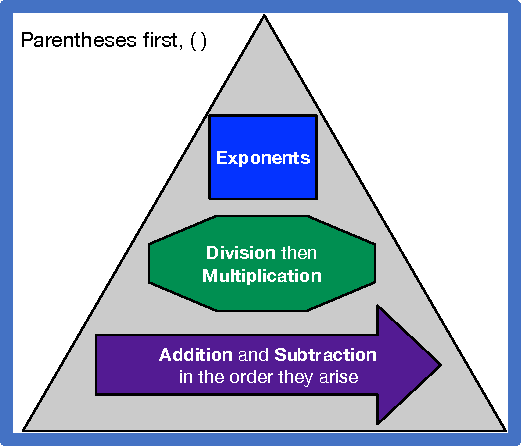
\includegraphics[width=\linewidth]{external/order-ops-pyr.pdf}
\end{sbspanel}%
\end{sidebyside}%
\tcblower
\end{figureptx}%
 \footnote{Resource: Bay-Williams, Jennifer M. and Sherri L. Martinie. \pubtitle{Order of Operations, The Myth and the Math}. Teaching Children Mathematics, Vol. 22, No. 1, August 2015.\label{g:fn:idp1871612792}}%
\end{subsectionptx}
%
%
\typeout{************************************************}
\typeout{Student Page 1.4.2 Three Threes}
\typeout{************************************************}
%
\newgeometry{left=1.2in, right=1.2in, top=1in, bottom=1in}
\begin{worksheet-subsection}{Three Threes}{}{Three Threes}{}{}{x:worksheet:act-three-threes}
\begin{introduction}{}%
Consider the Three Threes Clock Face in \hyperref[x:figure:fig-three-threes]{Figure~{\xreffont\ref{x:figure:fig-three-threes}}}. Verify that each number on the clock face is represented correctly using three threes. Think about how you are using the Order of Operations to check each expression. Use your creativity to find as many expressions for each number as you can.%
\begin{figureptx}{Three Threes Clock Face}{x:figure:fig-three-threes}{}%
\begin{image}{0.25}{0.5}{0.25}%
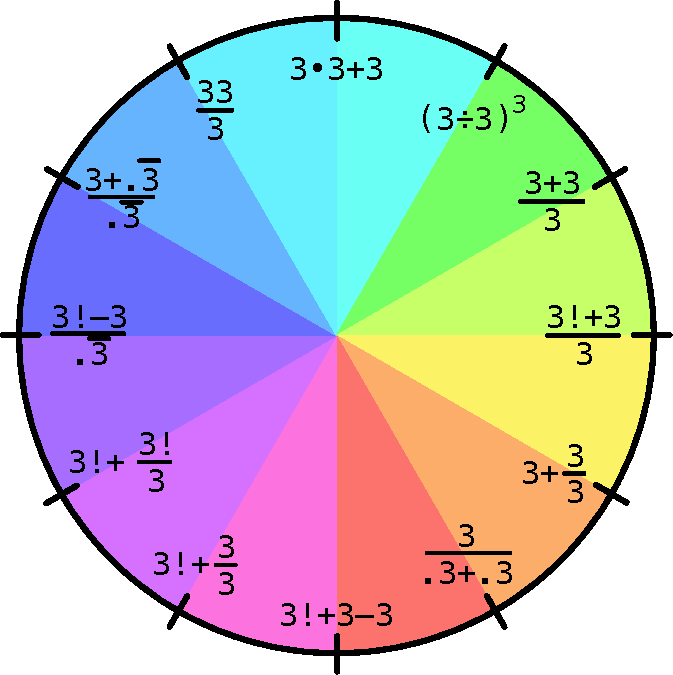
\includegraphics[width=\linewidth]{external/three-threes.pdf}
\end{image}%
\tcblower
\end{figureptx}%
\end{introduction}%
\begin{divisionexercise}{1}{}{}{g:exercise:idp1871609464}%
Verify that each expression is correct. Show your work. (As they arise, write any questions you have about any of the expressions.)%
\end{divisionexercise}%
\begin{divisionexercise}{2}{}{}{g:exercise:idp1871608312}%
Find other expressions for some of the numbers 1 through 12 using three threes. Show your work.%
\end{divisionexercise}%
\begin{conclusion}{}%
Share your thoughts on how each number on the clock was represented by three threes. Also share alternative ways you represented some of the numbers using three threes.%
\end{conclusion}%
\end{worksheet-subsection}
\restoregeometry
%
%
\typeout{************************************************}
\typeout{Student Page 1.4.3 Four Fours}
\typeout{************************************************}
%
\newgeometry{left=1.2in, right=1.2in, top=1in, bottom=1in}
\begin{worksheet-subsection}{Four Fours}{}{Four Fours}{}{}{x:worksheet:act-four-fours}
\begin{introduction}{}%
Now that you've had a chance to verify and play with expressions for the numbers 1 through 12 created using three threes, use your creativity to find expressions for other numbers using four fours. The Four Fours Problem provides you additional opportunities to think about the order of operations and the mathematical operations you have studied in previous courses. Study the problem presented below.%
\par
How can you make the numbers 1 through 20, 24, 30, and 100 using 4 fours? Record all of the expressions you find for each number in the table. Work alone for at least 5 minutes before you share your results with your group. If you get stuck, consult \hyperref[x:figure:fig-three-threes]{Figure~{\xreffont\ref{x:figure:fig-three-threes}}} for inspiration.%
\par
Use the number 4 exactly four times to write expressions equivalent to the numbers from 0 through 20. You may use any of the mathematical symbols below. A few examples are provided.%
\begin{itemize}[label=\textbullet]
\item{}Arithmetic operations: \(+, -, \times, \div\)%
\item{}Parentheses: ( )%
\item{}Decimal points or percents: e.g.\@ \(4.4\), \(.44\), 44\%%
\item{}Exponentiation: \textasciicircum{} (to the power of), e.g.\@ \((4 + 4)^4\)%
\item{}Square root: e.g.\@ \(\sqrt{4}\)%
\item{}Factorial: ! (\(4! = (4)(3)(2)(1) = 24\)%
\item{}Concatenation: e.g.\@ 44, 444%
\item{}Repeating decimal: \(. \overline{4} = \frac{4}{9}\)%
\end{itemize}
%
\end{introduction}%
\begin{divisionexercise}{1}{}{}{g:exercise:idp1871628792}%
Complete the table. Find at least one expression using 4 fours for each number. Use the Order of Operations; include grouping symbols as needed. Check your responses using a graphing calculator. Some examples for \(n = 4\) are provided. For the numbers whose solutions are shown in the table, find at least one more expression that works.%
\begin{center}%
{\tabularfont%
\begin{tabular}{Aclcl}\hrulethin
\multicolumn{1}{AcA}{\textbf{Number}}&\multicolumn{1}{cB}{\textbf{Four Fours Equation}}&\multicolumn{1}{cA}{\textbf{Number}}&\multicolumn{1}{cA}{\textbf{Four Fours Equation}}\tabularnewline\hrulemedium
\multicolumn{1}{AcA}{0}&\multicolumn{1}{lB}{}&\multicolumn{1}{cA}{12}&\multicolumn{1}{lA}{}\tabularnewline\hrulethin
\multicolumn{1}{AcA}{1}&\multicolumn{1}{lB}{\(1 = \left(\frac{4}{4} \right) ^{44}\)}&\multicolumn{1}{cA}{13}&\multicolumn{1}{lA}{}\tabularnewline\hrulethin
\multicolumn{1}{AcA}{2}&\multicolumn{1}{lB}{}&\multicolumn{1}{cA}{14}&\multicolumn{1}{lA}{}\tabularnewline\hrulethin
\multicolumn{1}{AcA}{3}&\multicolumn{1}{lB}{}&\multicolumn{1}{cA}{15}&\multicolumn{1}{lA}{\(15 = \frac{44}{4} + 4\)}\tabularnewline\hrulethin
\multicolumn{1}{AcA}{4}&\multicolumn{1}{lB}{}&\multicolumn{1}{cA}{16}&\multicolumn{1}{lA}{}\tabularnewline\hrulethin
\multicolumn{1}{AcA}{5}&\multicolumn{1}{lB}{}&\multicolumn{1}{cA}{17}&\multicolumn{1}{lA}{}\tabularnewline\hrulethin
\multicolumn{1}{AcA}{6}&\multicolumn{1}{lB}{}&\multicolumn{1}{cA}{18}&\multicolumn{1}{lA}{}\tabularnewline\hrulethin
\multicolumn{1}{AcA}{7}&\multicolumn{1}{lB}{\(7 = 4 + 4 - \frac{4}{4}\)}&\multicolumn{1}{cA}{19}&\multicolumn{1}{lA}{}\tabularnewline\hrulethin
\multicolumn{1}{AcA}{8}&\multicolumn{1}{lB}{}&\multicolumn{1}{cA}{20}&\multicolumn{1}{lA}{}\tabularnewline\hrulethin
\multicolumn{1}{AcA}{9}&\multicolumn{1}{lB}{}&\multicolumn{1}{cA}{24}&\multicolumn{1}{lA}{\(24 = 4! \cdot \left(\frac{\sqrt{4} \times \sqrt{4}}{4} \right)\)}\tabularnewline\hrulethin
\multicolumn{1}{AcA}{10}&\multicolumn{1}{lB}{}&\multicolumn{1}{cA}{30}&\multicolumn{1}{lA}{}\tabularnewline\hrulethin
\multicolumn{1}{AcA}{11}&\multicolumn{1}{lB}{}&\multicolumn{1}{cA}{100}&\multicolumn{1}{lA}{}\tabularnewline\hrulethin
\end{tabular}
}%
\end{center}%
\end{divisionexercise}%
\begin{divisionexercise}{2}{}{}{g:exercise:idp1871651448}%
What strategies did you use to find solutions?%
\end{divisionexercise}%
\begin{divisionexercise}{3}{}{}{g:exercise:idp1871653368}%
Find more than one solution for at least 3 of the numbers. Record them in the table.%
\end{divisionexercise}%
\begin{divisionexercise}{4}{}{}{g:exercise:idp1871656696}%
Which of your solutions are not dependent on the number 4?  For example \(1=\ \left(\frac{4}{4}\right)^{44}\) is also true when each 4 is replaced with 2, 6, or 9.  Highlight these solutions in your table.%
\end{divisionexercise}%
\begin{conclusion}{}%
Share the expressions you found using Four Fours with your group. Compare your work with your group members. Do you agree that each expression is correct? Circle any expressions you question; put a checkmark next to expressions with which you agree. Resolve any differences of opinion. When asked to do so, share some of your group's expressions with the class.%
\end{conclusion}%
\end{worksheet-subsection}
\restoregeometry
%
%
\typeout{************************************************}
\typeout{Homework 1.4.4 Homework}
\typeout{************************************************}
%
\begin{exercises-subsection}{Homework}{}{Homework}{}{}{x:exercises:hmwk-14}
\begin{introduction}{}%
Complete the following homework before the next class period:%
\end{introduction}%
\begin{divisionexercise}{1}{}{}{g:exercise:idp1871657080}%
Go back to \hyperlink{x:paragraphs:htlmfs-directions}{How To Learn Math For Students Directions}. Complete \hyperref[x:exercise:main-prob-four]{How to Learn Math for Students Exercise~{\xreffont\ref{x:exercise:main-prob-four}}}. You will hand in your written reflections for \hyperref[x:exercise:main-prob-four]{How to Learn Math for Students Exercise~{\xreffont\ref{x:exercise:main-prob-four}}} in class.%
\end{divisionexercise}%
\begin{divisionexercise}{2}{}{}{x:exercise:exer-14-2}%
Determine the value of each expression without the use of an electronic tool. Show your work one step at a time.%
\begin{enumerate}[font=\bfseries,label=(\alph*),ref=\alph*]
\item\label{x:task:exer-14-2a}\(4! - \left(4/ \sqrt{4} \right)^{4}\)%
\item{}\(4 + 4 / \sqrt{4} \times \sqrt{4}\)%
\end{enumerate}
\end{divisionexercise}%
\begin{divisionexercise}{3}{}{}{g:exercise:idp1871659128}%
While working on \hyperref[x:worksheet:act-four-fours]{Four Fours}, students solved the following expression in these four ways.%
\begin{align*}
\amp 4 + 4 / \sqrt{4} \times \sqrt{4} \amp \amp 4 + 4 / \sqrt{4} \times \sqrt{4} \amp \amp 4 + 4 / \sqrt{4} \times \sqrt{4} \amp \amp 4 + 4 / \sqrt{4} \times \sqrt{4}\\
\amp = 4 + 4 / 2 \times 2 \amp \amp = 4 + 4 / 2 \times 2 \amp \amp = 4 + 4 / 2 \times 2 \amp \amp = 4 + 4 / 2 \times 2\\
\amp = 4 + 4 / 4 \amp \amp = 8 / 4 \amp \amp = 4 + 2 \times 2 \amp \amp = 4 + 2 \times 2\\
\amp = 4 + 1 \amp \amp = 2 \amp \amp = 4 + 4 \amp \amp = 6 \times 2\\
\amp = 5 \amp \amp \amp \amp = 8 \amp \amp = 12
\end{align*}
%
\begin{enumerate}[font=\bfseries,label=(\alph*),ref=\alph*]
\item{}Only one solution can be correct. Which one is it? How do you know?%
\item{}For the solutions above that are incorrect, identify the error(s) the student made.%
\item{}As you work on \hyperref[x:worksheet:act-four-fours]{Four Fours} check the expressions you find to make sure they work for the numbers you think they do.%
\end{enumerate}
\end{divisionexercise}%
\begin{divisionexercise}{4}{}{}{g:exercise:idp1871686376}%
Solve each of the following. Show how you know your work is correct.%
\begin{enumerate}[font=\bfseries,label=(\alph*),ref=\alph*]
\item{}Insert parentheses so this equation is true: \(4 + 4 \div .4 \div \sqrt{4} = 7\).%
\item{}Insert parentheses so this equation is true: \(\sqrt{4}^{\sqrt{4}} + \sqrt{4} / 4 = 4\).%
\item{}Revisit \hyperref[x:task:exer-14-2a]{Task~{\xreffont 1.4.4.2}.{\xreffont\ref{x:task:exer-14-2a}}}. With no parentheses in the left side of the equation, what would the simplification of the expression be? Write the expression and show the simplification.%
\end{enumerate}
\end{divisionexercise}%
\begin{divisionexercise}{5}{}{}{g:exercise:idp1871688808}%
Look back at your work on the Four Fours Problem. Indicate where you used the mathematical properties and operations listed:%
\begin{itemize}[label=\textbullet]
\item{}Order of Operations%
\item{}Additive identity (adding zero, \(4 +(4 - 4) = 4 + 0 = 4\); \(\frac{4}{4}+(4-4)=1+0=1)\))%
\item{}Multiplicative identity (multiplying by \(1= \frac{4}{4}=\frac{4}{\sqrt4\sqrt4}\) )%
\item{}Fractions as divison, \(\frac{44}{4} = 11\)%
\item{}Square root: \(\sqrt{4} = 2\)%
\item{}Exponentiation: \(4^{\sqrt4}=4^2=4 \cdot 4=16\)%
\item{}Factorials: \(4! = 4 \cdot 3 \cdot 2 \cdot 1 = 24\)%
\item{}Concatenation: 44, 444%
\item{}Decimals: \(4.4, .4, . \overline{4} = .4444444\) \textellipsis{}%
\end{itemize}
%
\end{divisionexercise}%
\begin{divisionexercise}{6}{}{}{g:exercise:idp1871696360}%
What strategies have you used to find different expressions? Describe at least three.%
\end{divisionexercise}%
\begin{divisionexercise}{7}{}{}{g:exercise:idp1871692264}%
Which of the expressions you found will give you the same result if you use four copies of another number such as 1, 2, 3, \textellipsis{}? For example, \(\frac{4}{4}+\frac{4}{4}=2\); notice that this relationship also works if you replace all 4 fours with four of any of these single digit numbers: 1, 2, 3, 5, 6, 7, 8, or 9.%
\end{divisionexercise}%
\begin{divisionexercise}{8}{}{}{g:exercise:idp1871704552}%
Two students' work on the same math problem is shown below. Assess their work.%
\begin{align*}
\amp \text{Student 1:} \amp \amp \text{Student 2:}\\
\amp \sqrt{49} - 4 \div 2 + 3! \amp \amp \sqrt{49} - 4 \div 2 + 3!\\
\amp = 7 - 4 \div 2 + 3! \amp \amp = 7 - 4 \div 2 + 6\\
\amp = 7 - 4 \div 2 + 6 \amp \amp = 3 \div 2 +6\\
\amp = 7 - 4 \div 8 \amp \amp = 1.5 + 6\\
\amp = 3 \div 8 \amp \amp = 7.5\\
\amp = \frac{3}{8} \amp \amp
\end{align*}
%
\begin{enumerate}[font=\bfseries,label=(\alph*),ref=\alph*]
\item{}What error(s), if any, did each student make?%
\item{}If neither solution is correct, find the correct solution and show how to find it step-by-step.%
\end{enumerate}
\end{divisionexercise}%
\end{exercises-subsection}
\end{sectionptx}
%
%
\typeout{************************************************}
\typeout{Section 1.5 Four Fours Problem, Extended}
\typeout{************************************************}
%
\begin{sectionptx}{Four Fours Problem, Extended}{}{Four Fours Problem, Extended}{}{}{x:section:S_fours_extend}
%
%
\typeout{************************************************}
\typeout{Subsection 1.5.1 Overview}
\typeout{************************************************}
%
\begin{subsectionptx}{Overview}{}{Overview}{}{}{g:subsection:idp1871702248}
The section expands upon the ideas in \hyperref[x:section:S_orderofop]{Section~{\xreffont\ref{x:section:S_orderofop}}} by exploring other ways to use fours to make other numbers.%
\end{subsectionptx}
%
%
\typeout{************************************************}
\typeout{Student Page 1.5.2 Organizing Your Work: Ways to Use 1, 2, or 3 Fours to Make Other Numbers}
\typeout{************************************************}
%
\newgeometry{left=1.2in, right=1.2in, top=1in, bottom=1in}
\begin{worksheet-subsection}{Organizing Your Work: Ways to Use 1, 2, or 3 Fours to Make Other Numbers}{}{Organizing Your Work: Ways to Use 1, 2, or 3 Fours to Make Other Numbers}{}{}{x:worksheet:act-organize}
\begin{introduction}{}%
In mathematics, it is often helpful to create an organized list. \hyperref[x:worksheet:act-organize]{Organizing Your Work: Ways to Use 1, 2, or 3 Fours to Make Other Numbers} helps you organize expressions you have found using fewer than 4 fours.%
\end{introduction}%
\begin{divisionexercise}{1}{}{}{g:exercise:idp1871713128}%
As you worked on the Four Fours Problem, you likely found many ways to combine fewer than 4 fours. Use this table to organize what you've found. Find other ways to combine 1, 2, or 3 fours to make other numbers. For each column, order the combinations you find least to greatest.%
\begin{center}%
{\tabularfont%
\begin{tabular}{Alll}\hrulethin
\multicolumn{1}{AcA}{\textbf{Using 1 Four}}&\multicolumn{1}{cA}{\textbf{Using 2 Fours}}&\multicolumn{1}{cA}{\textbf{Using 3 Fours}}\tabularnewline\hrulethin
\multicolumn{1}{AlA}{~}&\multicolumn{1}{lA}{~}&\multicolumn{1}{lA}{~}\tabularnewline\hrulethin
\multicolumn{1}{AlA}{~}&\multicolumn{1}{lA}{~}&\multicolumn{1}{lA}{~}\tabularnewline\hrulethin
\multicolumn{1}{AlA}{~}&\multicolumn{1}{lA}{~}&\multicolumn{1}{lA}{~}\tabularnewline\hrulethin
\multicolumn{1}{AlA}{~}&\multicolumn{1}{lA}{~}&\multicolumn{1}{lA}{~}\tabularnewline\hrulethin
\multicolumn{1}{AlA}{~}&\multicolumn{1}{lA}{~}&\multicolumn{1}{lA}{~}\tabularnewline\hrulethin
\multicolumn{1}{AlA}{~}&\multicolumn{1}{lA}{~}&\multicolumn{1}{lA}{~}\tabularnewline\hrulethin
\multicolumn{1}{AlA}{~}&\multicolumn{1}{lA}{~}&\multicolumn{1}{lA}{~}\tabularnewline\hrulethin
\multicolumn{1}{AlA}{~}&\multicolumn{1}{lA}{~}&\multicolumn{1}{lA}{~}\tabularnewline\hrulethin
\multicolumn{1}{AlA}{~}&\multicolumn{1}{lA}{~}&\multicolumn{1}{lA}{~}\tabularnewline\hrulethin
\multicolumn{1}{AlA}{~}&\multicolumn{1}{lA}{~}&\multicolumn{1}{lA}{~}\tabularnewline\hrulethin
\multicolumn{1}{AlA}{~}&\multicolumn{1}{lA}{~}&\multicolumn{1}{lA}{~}\tabularnewline\hrulethin
\multicolumn{1}{AlA}{~}&\multicolumn{1}{lA}{~}&\multicolumn{1}{lA}{~}\tabularnewline\hrulethin
\multicolumn{1}{AlA}{~}&\multicolumn{1}{lA}{~}&\multicolumn{1}{lA}{~}\tabularnewline\hrulethin
\multicolumn{1}{AlA}{~}&\multicolumn{1}{lA}{~}&\multicolumn{1}{lA}{~}\tabularnewline\hrulethin
\end{tabular}
}%
\end{center}%
\end{divisionexercise}%
\begin{divisionexercise}{2}{}{}{g:exercise:idp1871724008}%
Combine some of the expressions you found in the table above to make numbers using four fours. How can this organized list help you find solutions for some of the numbers in \hyperref[x:worksheet:act-four-fours]{Four Fours}?%
\end{divisionexercise}%
\begin{divisionexercise}{3}{}{}{g:exercise:idp1871728104}%
What is the smallest number greater than zero you can make using four fours? What strategies did you use to find this number?%
\end{divisionexercise}%
\begin{divisionexercise}{4}{}{}{g:exercise:idp1871731176}%
What is the largest number you can make using four fours? What strategies did you use to find this number?%
\end{divisionexercise}%
\begin{conclusion}{}%
Share your solutions with your group. Verify each other's work. Get all possible answers on the board for the numbers 1 through 20, 24, 30, and 100. If there are any numbers for which solutions haven't been found, work on these together.%
\par
Once remaining questions about the Four Fours Problem are resolved, if time remains, work on \hyperref[x:worksheet:act-four-nums-prob]{Flexibility with Numbers: Four Numbers Problem} in your small group.%
\end{conclusion}%
\end{worksheet-subsection}
\restoregeometry
%
%
\typeout{************************************************}
\typeout{Homework 1.5.3 Homework}
\typeout{************************************************}
%
\begin{exercises-subsection}{Homework}{}{Homework}{}{}{g:exercises:idp1871732712}
\begin{divisionexercise}{1}{}{}{g:exercise:idp1871737832}%
Go back to \hyperlink{x:paragraphs:htlmfs-directions}{How To Learn Math For Students Directions}. Complete \hyperref[x:exercise:main-prob-five]{How to Learn Math for Students Exercise~{\xreffont\ref{x:exercise:main-prob-five}}}. You will hand in your written reflections for \hyperref[x:exercise:main-prob-five]{How to Learn Math for Students Exercise~{\xreffont\ref{x:exercise:main-prob-five}}} in class.%
\end{divisionexercise}%
\begin{divisionexercise}{2}{}{}{g:exercise:idp1871733864}%
The \hyperref[x:worksheet:act-four-nums-prob]{Flexibility with Numbers: Four Numbers Problem} extends \hyperref[x:worksheet:act-four-fours]{Four Fours}, this time using four copies of the same number. Your group will choose one of the numbers 1, 2, 3, 5, 6, 7, 8, or 9 (no group may choose the same number as another group). This is your first group assignment. Most of the work on this group assignment will occur outside of class. Exchange contact information and arrange times to get together electronically or in person to work on this assignment.%
\par
Your group's chosen number is \fillin{4.545454545454546}.%
\par
The completed \hyperref[x:worksheet:act-four-nums-prob]{Flexibility with Numbers: Four Numbers Problem} is due in class on \fillin{4.545454545454546}.%
\end{divisionexercise}%
\begin{divisionexercise}{3}{}{}{g:exercise:idp1871734504}%
Adapt \hyperref[x:worksheet:act-organize]{Organizing Your Work: Ways to Use 1, 2, or 3 Fours to Make Other Numbers} to help you solve \hyperref[x:worksheet:act-four-nums-prob]{Flexibility with Numbers: Four Numbers Problem}.%
\end{divisionexercise}%
\begin{divisionexercise}{4}{}{}{g:exercise:idp1871740776}%
Once you complete the \hyperref[x:worksheet:act-four-nums-prob]{Flexibility with Numbers: Four Numbers Problem}, you will also submit a reflection about how well your group worked together to solve the \hyperref[x:worksheet:act-four-nums-prob]{Flexibility with Numbers: Four Numbers Problem}. Answer the following questions to reflect on your work as a group. Turn in this reflection on the day you submit your group report for the \hyperref[x:worksheet:act-four-nums-prob]{Flexibility with Numbers: Four Numbers Problem}.%
\begin{enumerate}[font=\bfseries,label=(\alph*),ref=\alph*]
\item{}Did you and your group members get together outside of class or communicate outside of class to complete the work on the \hyperref[x:worksheet:act-four-nums-prob]{Flexibility with Numbers: Four Numbers Problem}?%
\item{}Did each group member come prepared to group meetings ready to contribute individual work to the group discussion?%
\item{}Did some group members only work on the problem when you were together? If so, characterize their contributions.%
\item{}What steps can your group take to help your group work more productively together?%
\item{}Are you satisfied with your group? If not, what would need to happen for you to be satisfied with your group?%
\item{}Would you like to stay with your current group? If you want to switch groups, with whom would you like to work?%
\end{enumerate}
\end{divisionexercise}%
\end{exercises-subsection}
%
%
\typeout{************************************************}
\typeout{Student Page 1.5.4 Flexibility with Numbers: Four Numbers Problem}
\typeout{************************************************}
%
\newgeometry{left=1.2in, right=1.2in, top=1in, bottom=1in}
\begin{worksheet-subsection}{Flexibility with Numbers: Four Numbers Problem}{}{Flexibility with Numbers: Four Numbers Problem}{}{}{x:worksheet:act-four-nums-prob}
\begin{introduction}{}%
Use the same number exactly four times to write expressions equivalent to the numbers 0 through 20. You may use any of the mathematical symbols below. A few examples for the number 4 are provided. Choose the number you will use and tell your instructor. You may choose one of the numbers: 1, 2, 3, 5, 6, 7, 8, 9. (Note that you may not use the number 4.)%
\begin{itemize}[label=\textbullet]
\item{}Arithmetic operations: \(+, -, \times, \div\)%
\item{}Parentheses: ( )%
\item{}Decimal points or percents: e.g.\@ \(4.4\), \(.44\), 44\%%
\item{}Exponentiation: \textasciicircum{} (to the power of), e.g.\@ \((4 + 4)^4\)%
\item{}Square root: e.g.\@ \(\sqrt{4}\)%
\item{}Factorial: ! (\(4! = (4)(3)(2)(1) = 24\)%
\item{}Concatenation: e.g.\@ 44, 444%
\item{}Repeating decimal: \(. \overline{4} = \frac{4}{9}\)%
\end{itemize}
%
\end{introduction}%
\begin{divisionexercise}{1}{}{}{g:exercise:idp1871760616}%
Complete the table writing solutions as expressions.  Use the Order of Operations; include grouping symbols as needed.  Check your responses using a calculator.  Some examples for the number 4 are provided. Your group's number is \fillin{4.545454545454546}.%
\begin{center}%
{\tabularfont%
\begin{tabular}{Aclcl}\hrulethin
\multicolumn{1}{AcA}{\textbf{Number}}&\multicolumn{1}{cB}{\textbf{Four Fours Equation}}&\multicolumn{1}{cA}{\textbf{Number}}&\multicolumn{1}{cA}{\textbf{Four Fours Equation}}\tabularnewline\hrulemedium
\multicolumn{1}{AcA}{0}&\multicolumn{1}{lB}{}&\multicolumn{1}{cA}{12}&\multicolumn{1}{lA}{}\tabularnewline\hrulethin
\multicolumn{1}{AcA}{1}&\multicolumn{1}{lB}{\(1 = \left(\frac{4}{4} \right) ^{44}\)}&\multicolumn{1}{cA}{13}&\multicolumn{1}{lA}{}\tabularnewline\hrulethin
\multicolumn{1}{AcA}{2}&\multicolumn{1}{lB}{}&\multicolumn{1}{cA}{14}&\multicolumn{1}{lA}{}\tabularnewline\hrulethin
\multicolumn{1}{AcA}{3}&\multicolumn{1}{lB}{}&\multicolumn{1}{cA}{15}&\multicolumn{1}{lA}{\(15 = \frac{44}{4} + 4\)}\tabularnewline\hrulethin
\multicolumn{1}{AcA}{4}&\multicolumn{1}{lB}{}&\multicolumn{1}{cA}{16}&\multicolumn{1}{lA}{}\tabularnewline\hrulethin
\multicolumn{1}{AcA}{5}&\multicolumn{1}{lB}{}&\multicolumn{1}{cA}{17}&\multicolumn{1}{lA}{}\tabularnewline\hrulethin
\multicolumn{1}{AcA}{6}&\multicolumn{1}{lB}{}&\multicolumn{1}{cA}{18}&\multicolumn{1}{lA}{}\tabularnewline\hrulethin
\multicolumn{1}{AcA}{7}&\multicolumn{1}{lB}{\(7 = 4 + 4 - \frac{4}{4}\)}&\multicolumn{1}{cA}{19}&\multicolumn{1}{lA}{}\tabularnewline\hrulethin
\multicolumn{1}{AcA}{8}&\multicolumn{1}{lB}{}&\multicolumn{1}{cA}{20}&\multicolumn{1}{lA}{}\tabularnewline\hrulethin
\multicolumn{1}{AcA}{9}&\multicolumn{1}{lB}{}&\multicolumn{1}{cA}{24}&\multicolumn{1}{lA}{\(24 = 4! \cdot \left(\frac{\sqrt{4} \times \sqrt{4}}{4} \right)\)}\tabularnewline\hrulethin
\multicolumn{1}{AcA}{10}&\multicolumn{1}{lB}{}&\multicolumn{1}{cA}{30}&\multicolumn{1}{lA}{}\tabularnewline\hrulethin
\multicolumn{1}{AcA}{11}&\multicolumn{1}{lB}{}&\multicolumn{1}{cA}{100}&\multicolumn{1}{lA}{}\tabularnewline\hrulethin
\end{tabular}
}%
\end{center}%
\end{divisionexercise}%
\begin{divisionexercise}{2}{}{}{g:exercise:idp1871785704}%
What strategies did you use to find solutions?%
\end{divisionexercise}%
\begin{divisionexercise}{3}{}{}{g:exercise:idp1871780840}%
Find more than one solution for at least 3 of the numbers.%
\end{divisionexercise}%
\begin{divisionexercise}{4}{}{}{g:exercise:idp1871785832}%
Which of your solutions are not dependent on the number you chose? Highlight these solutions in your table.%
\end{divisionexercise}%
\end{worksheet-subsection}
\restoregeometry
\begin{activity}{Summarizing Your Work on the Four Numbers Problem.}{x:activity:act-sum-four-nums}%
Use \hyperref[x:worksheet:act-reflect-fournums]{Reflecting on Your Group's Work on the Four Numbers Problem} to guide your group's reflection on your work on \hyperref[x:worksheet:act-four-nums-prob]{Flexibility with Numbers: Four Numbers Problem}. Look for similarities in how numbers were created. Keeping the Order of Operations in mind, check each other's solutions to see if you agree. Resolve disagreements.%
\begin{enumerate}[font=\bfseries,label=(\alph*),ref=\alph*]
\item{}Write a paragraph together indicating what you individually and collectively learned about some mathematical ideas through your individual and group work on the collection of activities:%
\begin{itemize}[label=\textbullet]
\item{}\hyperref[x:worksheet:act-three-threes]{Three Threes}%
\item{}\hyperref[x:worksheet:act-four-fours]{Four Fours}%
\item{}\hyperref[x:worksheet:act-organize]{Organizing Your Work: Ways to Use 1, 2, or 3 Fours to Make Other Numbers}, and%
\item{}\hyperref[x:worksheet:act-four-nums-prob]{Flexibility with Numbers: Four Numbers Problem}%
\end{itemize}
%
\item{}Write your name on your individual work and on the group reflection page. In your group, collect each member's work on the \hyperref[x:worksheet:act-four-nums-prob]{Flexibility with Numbers: Four Numbers Problem}. Staple \hyperref[x:worksheet:act-reflect-fournums]{Reflecting on Your Group's Work on the Four Numbers Problem} to the top of this collection to submit.%
\end{enumerate}
The Four Fours activities were designed to help you:%
\begin{itemize}[label=\textbullet]
\item{}Have fun with mathematics,%
\item{}See how mathematics can be a puzzle to play with,%
\item{}Experience how flexible problem solving can be (There were many expressions for each number, allowing you to use your creativity to find them.),%
\item{}Persevere in mathematics when you get stuck,%
\item{}Review and remember the Order of Operations,%
\item{}Recall and use many mathematical operations (+, \(-\), \texttimes{}, \(\div\), !, exponentiation),%
\item{}Become more familiar with your graphing calculator;s operation, and%
\item{}Experience generalization; several numbers could be expressed in the same way using any single digit integer.%
\end{itemize}
%
\par
One example of generalization in the \hyperref[x:worksheet:act-four-nums-prob]{Flexibility with Numbers: Four Numbers Problem} is: \(2=\frac{1+1}{\sqrt1\sqrt1}=\frac{4+4}{\sqrt4\sqrt4}=\frac{5+5}{\sqrt5\sqrt5}=\frac{8+8}{\sqrt8\sqrt8}=\frac{9+9}{\sqrt9\sqrt9}\). This equation works in the same way for 2, 3, 6, and 7. If you replace each numeral with 0! = 1, the number 2 can be represented in this way for 0! and all integers 1 through 9. To generalize this equation, we let n represent any single digit non-zero integer and replace the numerals in the equation with n. The equation becomes \(2=\frac{n+n}{\sqrt n\sqrt n}\) indicating that as long as each n in this equation is replaced by the same number, the equation is always equal to 2. The letter n is a variable. It takes the place of a number, allowing us to be free of having to show the equivalence using each number as we did at the beginning of this paragraph. This is a very powerful idea.%
\end{activity}%
%
%
\typeout{************************************************}
\typeout{Student Page 1.5.5 Reflecting on Your Group's Work on the Four Numbers Problem}
\typeout{************************************************}
%
\newgeometry{left=1.2in, right=1.2in, top=1in, bottom=1in}
\begin{worksheet-subsection}{Reflecting on Your Group's Work on the Four Numbers Problem}{}{Reflecting on Your Group's Work on the Four Numbers Problem}{}{}{x:worksheet:act-reflect-fournums}
\begin{divisionexercise}{1}{}{}{g:exercise:idp1871799528}%
Share your Four Numbers responses with your group. On your group member's sheet, highlight any expressions you find particularly interesting and any expressions you are unsure of so that you may discuss them together.%
\begin{enumerate}[font=\bfseries,label=(\alph*),ref=\alph*]
\item{}Do you agree with each of the solutions each group member found? If not, resolve any difficulties. Do not erase any of a student's original work. Instead, note any expressions over which group members had differences of opinion on the back of this page. Also indicate how you resolved them.%
\item{}Look for similarities in how numbers were created. What do you notice?%
\end{enumerate}
\end{divisionexercise}%
\begin{divisionexercise}{2}{}{}{g:exercise:idp1871803368}%
For which numbers did you and your group members have the most numerical expressions?%
\begin{enumerate}[font=\bfseries,label=(\alph*),ref=\alph*]
\item{}Write the numbers and as many different responses as you can in the table below.%
\begin{center}%
{\tabularfont%
\begin{tabular}{Allll}\hrulethin
\multicolumn{1}{AlA}{\textbf{Number}}&\multicolumn{1}{lA}{\textbf{Four Numbers Expression}}&\multicolumn{1}{lA}{\textbf{Number}}&\multicolumn{1}{lA}{\textbf{Four Numbers Expression}}\tabularnewline\hrulethin
\multicolumn{1}{AlA}{~}&\multicolumn{1}{lA}{~}&\multicolumn{1}{lA}{~}&\multicolumn{1}{lA}{~}\tabularnewline\hrulethin
\multicolumn{1}{AlA}{~}&\multicolumn{1}{lA}{~}&\multicolumn{1}{lA}{~}&\multicolumn{1}{lA}{~}\tabularnewline\hrulethin
\end{tabular}
}%
\end{center}%
\item{}What made these responses easy to find?%
\end{enumerate}
\end{divisionexercise}%
\begin{divisionexercise}{3}{}{}{g:exercise:idp1871808360}%
For which numbers did you and your group members have the smallest number of numerical expressions?%
\begin{enumerate}[font=\bfseries,label=(\alph*),ref=\alph*]
\item{}Write the numbers and the different responses group members found in the table below.%
\begin{center}%
{\tabularfont%
\begin{tabular}{Allll}\hrulethin
\multicolumn{1}{AlA}{\textbf{Number}}&\multicolumn{1}{lA}{\textbf{Four Numbers Expression}}&\multicolumn{1}{lA}{\textbf{Number}}&\multicolumn{1}{lA}{\textbf{Four Numbers Expression}}\tabularnewline\hrulethin
\multicolumn{1}{AlA}{~}&\multicolumn{1}{lA}{~}&\multicolumn{1}{lA}{~}&\multicolumn{1}{lA}{~}\tabularnewline\hrulethin
\multicolumn{1}{AlA}{~}&\multicolumn{1}{lA}{~}&\multicolumn{1}{lA}{~}&\multicolumn{1}{lA}{~}\tabularnewline\hrulethin
\end{tabular}
}%
\end{center}%
\item{}What made these responses difficult to find?%
\end{enumerate}
\end{divisionexercise}%
\begin{divisionexercise}{4}{}{}{g:exercise:idp1871815784}%
Were there any numbers for which your group found no numerical expressions using four numbers? Write the numbers below. We will work on these together as a class.%
\end{divisionexercise}%
\end{worksheet-subsection}
\restoregeometry
\end{sectionptx}
%
%
\typeout{************************************************}
\typeout{Section 1.6 Generalizations and Variables: Patterns in the 100s Chart}
\typeout{************************************************}
%
\begin{sectionptx}{Generalizations and Variables: Patterns in the 100s Chart}{}{Generalizations and Variables: Patterns in the 100s Chart}{}{}{x:section:S_patterns_100}
\begin{introduction}{}%
We saw that variables can be used to generalize expressions in \hyperref[x:worksheet:act-four-nums-prob]{Flexibility with Numbers: Four Numbers Problem} such as \(2=\frac{2+2}{\sqrt2\sqrt2}=\frac{6+6}{\sqrt6\sqrt6}=\frac{n+n}{\sqrt n\sqrt n}\). Variables can also be used in other ways. In this lesson, you will explore other ways that variables can be used in algebra.%
\end{introduction}%
%
%
\typeout{************************************************}
\typeout{Subsection 1.6.1 Video: Brains Grow and Change}
\typeout{************************************************}
%
\begin{subsectionptx}{Video: Brains Grow and Change}{}{Video: Brains Grow and Change}{}{}{x:subsection:SS_vid_brains}
The video explains that making sense of mathematics is necessary to grow your brain. It shares brain science related to how to strengthen or create new pathways in your brain. If somewhere in your past, you have gotten the idea that you are not a math person, this video might change your point of view! ``Brains Grow and Change'' is from \href{https://bhi61nm2cr3mkdgk1dtaov18-wpengine.netdna-ssl.com/wp-content/uploads/2015/06/Brains-Grow-Change.mp4}{YouCubed.org, Week 4 of Inspirational Math, Day 5}\footnote{\nolinkurl{bhi61nm2cr3mkdgk1dtaov18-wpengine.netdna-ssl.com/wp-content/uploads/2015/06/Brains-Grow-Change.mp4}\label{g:fn:idp1871823208}}.%
\end{subsectionptx}
%
%
\typeout{************************************************}
\typeout{Subsection 1.6.2 Number Talk: 43 \textminus{} 28}
\typeout{************************************************}
%
\begin{subsectionptx}{Number Talk: 43 \textminus{} 28}{}{Number Talk: 43 \textminus{} 28}{}{}{x:subsection:SS_nums_43_28}
Number talks help you realize how many different, correct, ways there are to solve the same problem. They help you develop flexibility with numbers. Eventually, we will look for generalizations, extending our number talks into algebra. Consider the following problem:%
\begin{assemblage}{}{g:assemblage:idp1871824616}%
I had \textdollar{}43 with me when I went shoping last week.%
\par
I spent \textdollar{}28 on fruit. How much do I have left?%
\par
Solve the problem mentally. Find at least one other way to solve the problem mentally. When asked to do so, share your solution and one of the ways you solved the problem.%
\end{assemblage}
When everyone is ready, you will be asked to share your solution. Once all solutions are expressed, you will take turns sharing solution processes you found. When sharing your solution process, answer the questions below:%
\begin{descriptionlist}
\begin{dlimedium}{Answer}{g:li:idp1871826280}%
Which solution are you defending?%
\end{dlimedium}%
\begin{dlimedium}{Ask}{g:li:idp1871824360}%
Does anyone have a question for me?%
\end{dlimedium}%
\begin{dlimedium}{Ask}{g:li:idp1871821288}%
Does anyone have another way to solve the problem?%
\end{dlimedium}%
\end{descriptionlist}
Remember, your brain grows when you make mistakes and even more when you resolve them.%
\end{subsectionptx}
%
%
\typeout{************************************************}
\typeout{Student Page 1.6.3 Analyzing the 100s Chart}
\typeout{************************************************}
%
\newgeometry{left=1.2in, right=1.2in, top=1in, bottom=1in}
\begin{worksheet-subsection}{Analyzing the 100s Chart}{}{Analyzing the 100s Chart}{}{}{x:worksheet:act-analyze100}
\begin{introduction}{}%
Generalization is an important concept in algebra. It is the basis of the use of variables. Think about what the word, variable, means when you are not thinking about mathematics. Share your ideas about this.%
\par
We will continue to refine our meaning of variable through today's activities. Work on \hyperref[x:worksheet:act-analyze100]{Analyzing the 100s Chart}. As with the Four Fours collection of activities, use your creativity. Work to give clear descriptions of any patterns you find. Color code each pattern and illustrate it in the same color on the 100s Chart.%
\end{introduction}%
\begin{divisionexercise}{1}{}{}{g:exercise:idp1871837160}%
Study \hyperref[x:table:hunds-chart]{Table~{\xreffont\ref{x:table:hunds-chart}}}.%
\begin{tableptx}{\textbf{The 100s Chart}}{x:table:hunds-chart}{}%
\centering%
{\tabularfont%
\begin{tabular}{Acccccccccc}\hrulethin
\multicolumn{1}{AcA}{100}&\multicolumn{1}{cA}{101}&\multicolumn{1}{cA}{102}&\multicolumn{1}{cA}{103}&\multicolumn{1}{cA}{104}&\multicolumn{1}{cA}{105}&\multicolumn{1}{cA}{106}&\multicolumn{1}{cA}{107}&\multicolumn{1}{cA}{108}&\multicolumn{1}{cA}{109}\tabularnewline\hrulethin
\multicolumn{1}{AcA}{90}&\multicolumn{1}{cA}{91}&\multicolumn{1}{cA}{92}&\multicolumn{1}{cA}{93}&\multicolumn{1}{cA}{94}&\multicolumn{1}{cA}{95}&\multicolumn{1}{cA}{96}&\multicolumn{1}{cA}{97}&\multicolumn{1}{cA}{98}&\multicolumn{1}{cA}{99}\tabularnewline\hrulethin
\multicolumn{1}{AcA}{80}&\multicolumn{1}{cA}{81}&\multicolumn{1}{cA}{82}&\multicolumn{1}{cA}{83}&\multicolumn{1}{cA}{84}&\multicolumn{1}{cA}{85}&\multicolumn{1}{cA}{86}&\multicolumn{1}{cA}{87}&\multicolumn{1}{cA}{88}&\multicolumn{1}{cA}{89}\tabularnewline\hrulethin
\multicolumn{1}{AcA}{70}&\multicolumn{1}{cA}{71}&\multicolumn{1}{cA}{72}&\multicolumn{1}{cA}{73}&\multicolumn{1}{cA}{74}&\multicolumn{1}{cA}{75}&\multicolumn{1}{cA}{76}&\multicolumn{1}{cA}{77}&\multicolumn{1}{cA}{78}&\multicolumn{1}{cA}{79}\tabularnewline\hrulethin
\multicolumn{1}{AcA}{60}&\multicolumn{1}{cA}{61}&\multicolumn{1}{cA}{62}&\multicolumn{1}{cA}{63}&\multicolumn{1}{cA}{64}&\multicolumn{1}{cA}{65}&\multicolumn{1}{cA}{66}&\multicolumn{1}{cA}{67}&\multicolumn{1}{cA}{68}&\multicolumn{1}{cA}{69}\tabularnewline\hrulethin
\multicolumn{1}{AcA}{50}&\multicolumn{1}{cA}{51}&\multicolumn{1}{cA}{52}&\multicolumn{1}{cA}{53}&\multicolumn{1}{cA}{54}&\multicolumn{1}{cA}{55}&\multicolumn{1}{cA}{56}&\multicolumn{1}{cA}{57}&\multicolumn{1}{cA}{58}&\multicolumn{1}{cA}{59}\tabularnewline\hrulethin
\multicolumn{1}{AcA}{40}&\multicolumn{1}{cA}{41}&\multicolumn{1}{cA}{42}&\multicolumn{1}{cA}{43}&\multicolumn{1}{cA}{44}&\multicolumn{1}{cA}{45}&\multicolumn{1}{cA}{46}&\multicolumn{1}{cA}{47}&\multicolumn{1}{cA}{48}&\multicolumn{1}{cA}{49}\tabularnewline\hrulethin
\multicolumn{1}{AcA}{30}&\multicolumn{1}{cA}{31}&\multicolumn{1}{cA}{32}&\multicolumn{1}{cA}{33}&\multicolumn{1}{cA}{34}&\multicolumn{1}{cA}{35}&\multicolumn{1}{cA}{36}&\multicolumn{1}{cA}{37}&\multicolumn{1}{cA}{38}&\multicolumn{1}{cA}{39}\tabularnewline\hrulethin
\multicolumn{1}{AcA}{20}&\multicolumn{1}{cA}{21}&\multicolumn{1}{cA}{22}&\multicolumn{1}{cA}{23}&\multicolumn{1}{cA}{24}&\multicolumn{1}{cA}{25}&\multicolumn{1}{cA}{26}&\multicolumn{1}{cA}{27}&\multicolumn{1}{cA}{28}&\multicolumn{1}{cA}{29}\tabularnewline\hrulethin
\multicolumn{1}{AcA}{10}&\multicolumn{1}{cA}{11}&\multicolumn{1}{cA}{12}&\multicolumn{1}{cA}{13}&\multicolumn{1}{cA}{14}&\multicolumn{1}{cA}{15}&\multicolumn{1}{cA}{16}&\multicolumn{1}{cA}{17}&\multicolumn{1}{cA}{18}&\multicolumn{1}{cA}{19}\tabularnewline\hrulethin
\multicolumn{1}{AcA}{0}&\multicolumn{1}{cA}{1}&\multicolumn{1}{cA}{2}&\multicolumn{1}{cA}{3}&\multicolumn{1}{cA}{4}&\multicolumn{1}{cA}{5}&\multicolumn{1}{cA}{6}&\multicolumn{1}{cA}{7}&\multicolumn{1}{cA}{8}&\multicolumn{1}{cA}{9}\tabularnewline\hrulethin
\end{tabular}
}%
\end{tableptx}%
\begin{enumerate}[font=\bfseries,label=(\alph*),ref=\alph*]
\item{}What must be added to a number to get the number immediately to its right?%
\item{}What must be added to a number to get the number directly below the number?%
\end{enumerate}
\end{divisionexercise}%
\begin{divisionexercise}{2}{}{}{g:exercise:idp1871880296}%
Replace 6 with the letter \(n\) so that \(n = 6\). When \(n = 6\), notice that \(7 = n + 1\). Rewrite 8 and 5 in terms of n where \(n = 6\). Also write the expressions in \hyperref[x:table:hunds-chart]{Table~{\xreffont\ref{x:table:hunds-chart}}}.%
\end{divisionexercise}%
\begin{divisionexercise}{3}{}{}{g:exercise:idp1871881576}%
Replace the number 23 with the letter \(m\) so that \(m = 23\). What are the next two odd numbers after 23? Write these odd numbers using the letter \(m\) instead of 23. Write the expressions in \hyperref[x:table:hunds-chart]{Table~{\xreffont\ref{x:table:hunds-chart}}}.%
\end{divisionexercise}%
\begin{divisionexercise}{4}{}{}{g:exercise:idp1871892328}%
How can you represent the number just below 23 on the 100s chart in terms of \(m\) where \(m = 23\)? How can you represent the number just above 23 on the 100s chart using \(m\)? Write the expressions in \hyperref[x:table:hunds-chart]{Table~{\xreffont\ref{x:table:hunds-chart}}}.%
\end{divisionexercise}%
\begin{divisionexercise}{5}{}{}{g:exercise:idp1871891688}%
Suppose \hyperref[x:table:hunds-subchart]{Table~{\xreffont\ref{x:table:hunds-subchart}}} is located somewhere in \hyperref[x:table:hunds-chart]{Table~{\xreffont\ref{x:table:hunds-chart}}}. Write each value in the rectangle in terms of \(x\).%
\begin{tableptx}{\textbf{100s Subchart}}{x:table:hunds-subchart}{}%
\centering%
{\tabularfont%
\begin{tabular}{Alll}\hrulethin
\multicolumn{1}{AlA}{~~~}&\multicolumn{1}{lA}{~~~}&\multicolumn{1}{lA}{~~~}\tabularnewline\hrulethin
\multicolumn{1}{AlA}{~~~}&\multicolumn{1}{lA}{\(x\)}&\multicolumn{1}{lA}{~~~}\tabularnewline\hrulethin
\multicolumn{1}{AlA}{~~~}&\multicolumn{1}{lA}{~~~}&\multicolumn{1}{lA}{~~~}\tabularnewline\hrulethin
\multicolumn{1}{AlA}{~}&\multicolumn{1}{lA}{~}&\multicolumn{1}{lA}{~}\tabularnewline\hrulethin
\end{tabular}
}%
\end{tableptx}%
\end{divisionexercise}%
\begin{divisionexercise}{6}{}{}{x:exercise:analyze100-x}%
Notice that every rectangle in \hyperref[x:table:hunds-chart]{Table~{\xreffont\ref{x:table:hunds-chart}}} with the same dimensions as \hyperref[x:table:hunds-subchart]{Table~{\xreffont\ref{x:table:hunds-subchart}}} can be labeled exactly the same way. The initial value of \(x\) is irrelevant. Why is that?%
\end{divisionexercise}%
\begin{divisionexercise}{7}{}{}{g:exercise:idp1871902824}%
What patterns do you see in \hyperref[x:table:hunds-chart]{Table~{\xreffont\ref{x:table:hunds-chart}}}? Find at least 3. Color code each pattern in the chart. Describe each pattern in writing. Include a description of how to move to successive numbers and how much is added or subtracted each time you make the move. Explain why the pattern works as you say it does.%
\end{divisionexercise}%
\begin{conclusion}{}%
For \hyperref[x:worksheet:act-analyze100]{Analyzing the 100s Chart}, share your solutions to each problem with your group. Share two of the more challenging patterns your group found with the class.%
\par
Of the patterns shared by the class, choose 2 to work on with your group. Together, describe the pattern carefully then figure out why each pattern works. Does the starting number matter? Be ready to share with the class.%
\end{conclusion}%
\end{worksheet-subsection}
\restoregeometry
%
%
\typeout{************************************************}
\typeout{Homework 1.6.4 Homework}
\typeout{************************************************}
%
\begin{exercises-subsection}{Homework}{}{Homework}{}{}{g:exercises:idp1871907176}
\begin{divisionexercise}{1}{}{}{g:exercise:idp1871905640}%
Go back to \hyperlink{x:paragraphs:htlmfs-directions}{How To Learn Math For Students Directions} from \hyperref[x:section:S_learnmath]{Section~{\xreffont\ref{x:section:S_learnmath}}}, How to Learn Math for Students. Complete \hyperref[x:exercise:main-prob-six]{How to Learn Math for Students Exercise~{\xreffont\ref{x:exercise:main-prob-six}}}. You will hand in your written reflections for \hyperref[x:exercise:main-prob-six]{How to Learn Math for Students Exercise~{\xreffont\ref{x:exercise:main-prob-six}}} in class.%
\end{divisionexercise}%
\begin{divisionexercise}{2}{}{}{x:exercise:exer-placeholder}%
Revisit \hyperlink{x:exercise:analyze100-x}{Student Page Exercise~{\xreffont 1.6.3.6}} in \hyperref[x:worksheet:act-analyze100]{Analyzing the 100s Chart}. Because the initial value of \(x\) is irrelevant, \(x\) is considered a variable. Once a particular value of \(x\) is chosen, then all of the values in the rectangle that are currently represented by expressions in terms of \(x\) can be determined. In this second case, \(x\) is a placeholder. Look at the expressions and equations below. For each, decide if \(x\) is a variable or if \(x\) is a placeholder.%
\begin{enumerate}[font=\bfseries,label=(\alph*),ref=\alph*]
\item{}\(x + 1 = 3\)%
\item{}\(x + 1 = y\)%
\item{}\(2x = x + 1\)%
\item{}\(2x - 1 = y\)%
\end{enumerate}
\end{divisionexercise}%
\begin{divisionexercise}{3}{}{}{x:exercise:exer-like-terms-tiles}%
You probably have learned to combine like terms in previous mathematics classes. As with the Order of Operations, there are mathematical reasons underlying which terms can be combined.%
\par
When children learn to multiply, they use arrays such as those in \hyperref[x:figure:fig-like-terms-array]{Figure~{\xreffont\ref{x:figure:fig-like-terms-array}}} to make sense of repeated addition. The product of the dimensions of an array is the number of squares in the array; the number of rows shows how many times the number of squares in the first row is repeated. \hyperref[x:worksheet:act-like-terms]{Combining Like Terms} builds on this experience in learning multiplication to help you think about the meaning of the terms 1, \(x\), and \(x^2\) in the context of area as you model expressions with algebra tiles. Complete \hyperref[x:worksheet:act-like-terms]{Combining Like Terms}. Write down any questions you have as you work so you can ask them in class.%
\begin{figureptx}{Like Terms Array}{x:figure:fig-like-terms-array}{}%
\begin{image}{0.25}{0.5}{0.25}%
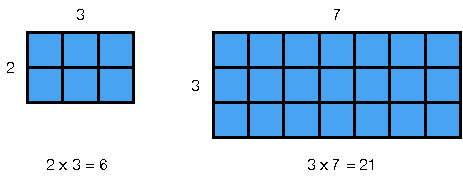
\includegraphics[width=\linewidth]{external/like-terms-array.pdf}
\end{image}%
\tcblower
\end{figureptx}%
\end{divisionexercise}%
\begin{divisionexercise}{4}{}{}{g:exercise:idp1871917032}%
There are free apps online to help you make sense of combining like terms and adding polynomials using algebra tiles. \href{http://media.mivu.org/mvu_pd/a4a/homework/index.html}{Use the apps on this website}\footnotemark{}. Read the introductory pages carefully. These pages tell you how to use the apps. Navigate through the introduction using the arrow in the upper right corner. Watch the videos and play with the apps for \pubtitle{Simplifying Expressions and Adding Polynomials}. Solve at least 2 problems at each difficulty level, until you conceptually understand the link between the algebra tiles and the expressions they represent. This work should take at most 20 minutes.%
\end{divisionexercise}%
\footnotetext[8]{\nolinkurl{media.mivu.org/mvu_pd/a4a/homework/index.html}\label{g:fn:idp1871920744}}%
\end{exercises-subsection}
%
%
\typeout{************************************************}
\typeout{Student Page 1.6.5 Combining Like Terms}
\typeout{************************************************}
%
\newgeometry{left=1.2in, right=1.2in, top=1in, bottom=1in}
\begin{worksheet-subsection}{Combining Like Terms}{}{Combining Like Terms}{}{}{x:worksheet:act-like-terms}
\begin{divisionexercise}{1}{}{}{g:exercise:idp1871922920}%
Find the area of each of the algebra tiles shown. The side lengths are labeled. The variable, \(x\), represents an unknown length.%
\begin{image}{0.25}{0.5}{0.25}%
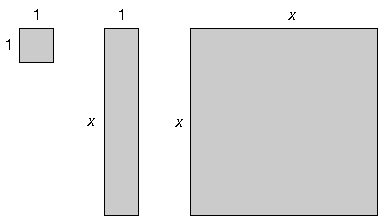
\includegraphics[width=\linewidth]{external/tiles-like-terms1.pdf}
\end{image}%
\end{divisionexercise}%
\begin{divisionexercise}{2}{}{}{g:exercise:idp1871921384}%
Translate each of the figures into algebra. Explain your translation. Simplify each expression as much as possible and explain why you cannot simplify further.%
\begin{enumerate}[font=\bfseries,label=(\alph*),ref=\alph*]
\item{}\begin{image}{0.35}{0.3}{0.35}%
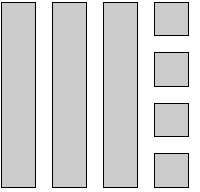
\includegraphics[width=\linewidth]{external/tiles-like-terms2a.pdf}
\end{image}%
\item{}\begin{image}{0.25}{0.5}{0.25}%
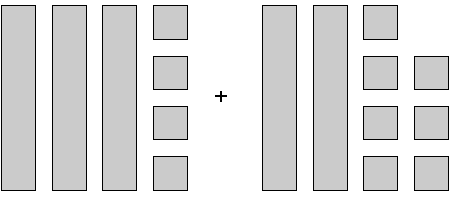
\includegraphics[width=\linewidth]{external/tiles-like-terms2b.pdf}
\end{image}%
\item{}\begin{image}{0.25}{0.5}{0.25}%
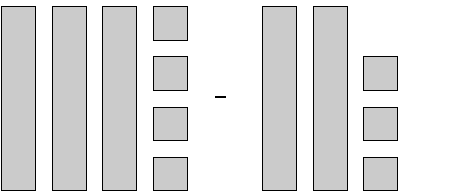
\includegraphics[width=\linewidth]{external/tiles-like-terms2c.pdf}
\end{image}%
\item{}\begin{image}{0.25}{0.5}{0.25}%
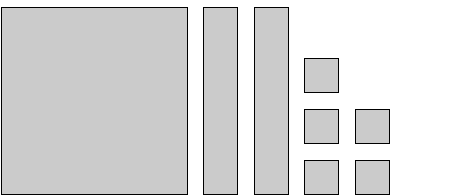
\includegraphics[width=\linewidth]{external/tiles-like-terms2d.pdf}
\end{image}%
\end{enumerate}
\end{divisionexercise}%
\begin{divisionexercise}{3}{}{}{g:exercise:idp1871924584}%
Draw algebra tiles to illustrate each expression. Use your illustration to simplify each of the algebraic expressions. Explain how you know you are correct.%
\begin{enumerate}[font=\bfseries,label=(\alph*),ref=\alph*]
\item{}\(2x + 4 + 3x + 7 =\)%
\item{}\(4x + 8 - 3x + 2 =\)%
\item{}\(3x + 8 - (4x + 2) =\)%
\item{}\(7x - 2(3x - 1) + x =\)%
\end{enumerate}
\end{divisionexercise}%
\begin{divisionexercise}{4}{}{}{g:exercise:idp1871931624}%
Summarize your work with combining like terms. Which terms can you combine? How do you know?%
\end{divisionexercise}%
\begin{divisionexercise}{5}{}{}{g:exercise:idp1871929192}%
Simplify the following expressions. Show and explain your work.%
\begin{enumerate}[font=\bfseries,label=(\alph*),ref=\alph*]
\item{}\(3 + 5x - x + 7 =\)%
\item{}\(3 + 5x - (x + 7) =\)%
\item{}\(4 + 2(x - 1) =\)%
\item{}\(15x - 4(2 - 3x) + 7 =\)%
\end{enumerate}
\end{divisionexercise}%
\end{worksheet-subsection}
\restoregeometry
\end{sectionptx}
%
%
\typeout{************************************************}
\typeout{Section 1.7 More with Patterns and Variables: Rectangular Patterns in the 100s Chart}
\typeout{************************************************}
%
\begin{sectionptx}{More with Patterns and Variables: Rectangular Patterns in the 100s Chart}{}{More with Patterns and Variables: Rectangular Patterns in the 100s Chart}{}{}{x:section:S_more_patterns}
\begin{introduction}{}%
Throughout this chapter, you have experienced how problems can be approached in a variety of ways. For example, to solve arithmetic problems such as 43 \textminus{} 28, students found at least 8 ways to do this. Using four fours and four numbers, you found many ways to express most of the numbers 1 through 20. You found many patterns in the 100s chart. By now, we hope you are finding that mathematics is a way of thinking and communicating that can be very creative. One of the hallmarks of mathematics is sense-making in your own way, not in a way prescribed for you. In this lesson you will use your creativity based in sense making to find more ways to simplify an arithmetic expression and look for more patterns in the 100s Chart.%
\end{introduction}%
%
%
\typeout{************************************************}
\typeout{Subsection 1.7.1 Number Talk: 93 \textminus{} 27}
\typeout{************************************************}
%
\begin{subsectionptx}{Number Talk: 93 \textminus{} 27}{}{Number Talk: 93 \textminus{} 27}{}{}{x:subsection:SS_nums93-27}
Solve the following problem in as many ways as you can.%
\begin{assemblage}{}{g:assemblage:idp1871936872}%
Mentally solve 93 \textminus{} 27 in as many ways as you can.%
\par
Raise a thumb when you have a solution. Raise a finger for each additional solution process you find.%
\end{assemblage}
One way a student solved 93 \textminus{} 27 was by adding 3 to both 93 and 27 to get 96 \textminus{} 30 = 66. The student also solved the problem by adding 4 to both numbers to get 97 \textminus{} 31 = 66. Does this strategy always work? Why or why not? Is the student's process related to the 100s chart? Find the numbers on \hyperref[x:table:hunds-chart]{Table~{\xreffont\ref{x:table:hunds-chart}}} and explain what's happening to the numbers. Use algebra to explain why this process works.%
\end{subsectionptx}
%
%
\typeout{************************************************}
\typeout{Student Page 1.7.2 Rectangle Patterns in the 100s Chart}
\typeout{************************************************}
%
\newgeometry{left=1.2in, right=1.2in, top=1in, bottom=1in}
\begin{worksheet-subsection}{Rectangle Patterns in the 100s Chart}{}{Rectangle Patterns in the 100s Chart}{}{}{x:worksheet:act-rec-patterns}
\begin{introduction}{}%
In \hyperref[x:worksheet:act-analyze100]{Analyzing the 100s Chart} you found patterns in rows, columns, or diagonals. This time your pattern search will be confined to rectangles.%
\end{introduction}%
\begin{divisionexercise}{1}{}{}{g:exercise:idp1871943784}%
Consider the rectangle in \hyperref[x:table:rec-patt-rectang]{Table~{\xreffont\ref{x:table:rec-patt-rectang}}}. What patterns do you see in the numbers in this rectangle?%
\begin{tableptx}{\textbf{Rectangle for Rectangle Patterns in the 100s Chart.}}{x:table:rec-patt-rectang}{}%
\centering%
{\tabularfont%
\begin{tabular}{Alll}\hrulethin
\multicolumn{1}{AlA}{84}&\multicolumn{1}{lA}{85}&\multicolumn{1}{lA}{86}\tabularnewline\hrulethin
\multicolumn{1}{AlA}{74}&\multicolumn{1}{lA}{75}&\multicolumn{1}{lA}{76}\tabularnewline\hrulethin
\multicolumn{1}{AlA}{64}&\multicolumn{1}{lA}{65}&\multicolumn{1}{lA}{66}\tabularnewline\hrulethin
\multicolumn{1}{AlA}{54}&\multicolumn{1}{lA}{55}&\multicolumn{1}{lA}{56}\tabularnewline\hrulethin
\end{tabular}
}%
\end{tableptx}%
Let \(x = 84\). In the rectangle, write the other values in the rectangle in terms of \(x\).%
\begin{enumerate}[font=\bfseries,label=(\alph*),ref=\alph*]
\item{}Use your relabeling to justify any numeric patterns you found.%
\item{}Find another pattern in the relabeled rectangle.%
\item{}Does your pattern work for a 4 by 3 rectangle with upper left corner labeled 51?%
\item{}Does your pattern work for any other 4 by 3 rectangles? Why or why not?%
\end{enumerate}
Work on the the following exercises alone for at least 10 minutes. When each member of your group has found at least one rectangle pattern, share the patterns you found with your group.%
\end{divisionexercise}%
\begin{divisionexercise}{2}{}{}{g:exercise:idp1872093672}%
Using a different color to outline each rectangle, draw three rectangles following the lines in \hyperref[x:table:hunds-chart]{Table~{\xreffont\ref{x:table:hunds-chart}}} (reprinted below) with the following rules:%
\begin{center}%
{\tabularfont%
\begin{tabular}{Acccccccccc}\hrulethin
\multicolumn{1}{AcA}{100}&\multicolumn{1}{cA}{101}&\multicolumn{1}{cA}{102}&\multicolumn{1}{cA}{103}&\multicolumn{1}{cA}{104}&\multicolumn{1}{cA}{105}&\multicolumn{1}{cA}{106}&\multicolumn{1}{cA}{107}&\multicolumn{1}{cA}{108}&\multicolumn{1}{cA}{109}\tabularnewline\hrulethin
\multicolumn{1}{AcA}{90}&\multicolumn{1}{cA}{91}&\multicolumn{1}{cA}{92}&\multicolumn{1}{cA}{93}&\multicolumn{1}{cA}{94}&\multicolumn{1}{cA}{95}&\multicolumn{1}{cA}{96}&\multicolumn{1}{cA}{97}&\multicolumn{1}{cA}{98}&\multicolumn{1}{cA}{99}\tabularnewline\hrulethin
\multicolumn{1}{AcA}{80}&\multicolumn{1}{cA}{81}&\multicolumn{1}{cA}{82}&\multicolumn{1}{cA}{83}&\multicolumn{1}{cA}{84}&\multicolumn{1}{cA}{85}&\multicolumn{1}{cA}{86}&\multicolumn{1}{cA}{87}&\multicolumn{1}{cA}{88}&\multicolumn{1}{cA}{89}\tabularnewline\hrulethin
\multicolumn{1}{AcA}{70}&\multicolumn{1}{cA}{71}&\multicolumn{1}{cA}{72}&\multicolumn{1}{cA}{73}&\multicolumn{1}{cA}{74}&\multicolumn{1}{cA}{75}&\multicolumn{1}{cA}{76}&\multicolumn{1}{cA}{77}&\multicolumn{1}{cA}{78}&\multicolumn{1}{cA}{79}\tabularnewline\hrulethin
\multicolumn{1}{AcA}{60}&\multicolumn{1}{cA}{61}&\multicolumn{1}{cA}{62}&\multicolumn{1}{cA}{63}&\multicolumn{1}{cA}{64}&\multicolumn{1}{cA}{65}&\multicolumn{1}{cA}{66}&\multicolumn{1}{cA}{67}&\multicolumn{1}{cA}{68}&\multicolumn{1}{cA}{69}\tabularnewline\hrulethin
\multicolumn{1}{AcA}{50}&\multicolumn{1}{cA}{51}&\multicolumn{1}{cA}{52}&\multicolumn{1}{cA}{53}&\multicolumn{1}{cA}{54}&\multicolumn{1}{cA}{55}&\multicolumn{1}{cA}{56}&\multicolumn{1}{cA}{57}&\multicolumn{1}{cA}{58}&\multicolumn{1}{cA}{59}\tabularnewline\hrulethin
\multicolumn{1}{AcA}{40}&\multicolumn{1}{cA}{41}&\multicolumn{1}{cA}{42}&\multicolumn{1}{cA}{43}&\multicolumn{1}{cA}{44}&\multicolumn{1}{cA}{45}&\multicolumn{1}{cA}{46}&\multicolumn{1}{cA}{47}&\multicolumn{1}{cA}{48}&\multicolumn{1}{cA}{49}\tabularnewline\hrulethin
\multicolumn{1}{AcA}{30}&\multicolumn{1}{cA}{31}&\multicolumn{1}{cA}{32}&\multicolumn{1}{cA}{33}&\multicolumn{1}{cA}{34}&\multicolumn{1}{cA}{35}&\multicolumn{1}{cA}{36}&\multicolumn{1}{cA}{37}&\multicolumn{1}{cA}{38}&\multicolumn{1}{cA}{39}\tabularnewline\hrulethin
\multicolumn{1}{AcA}{20}&\multicolumn{1}{cA}{21}&\multicolumn{1}{cA}{22}&\multicolumn{1}{cA}{23}&\multicolumn{1}{cA}{24}&\multicolumn{1}{cA}{25}&\multicolumn{1}{cA}{26}&\multicolumn{1}{cA}{27}&\multicolumn{1}{cA}{28}&\multicolumn{1}{cA}{29}\tabularnewline\hrulethin
\multicolumn{1}{AcA}{10}&\multicolumn{1}{cA}{11}&\multicolumn{1}{cA}{12}&\multicolumn{1}{cA}{13}&\multicolumn{1}{cA}{14}&\multicolumn{1}{cA}{15}&\multicolumn{1}{cA}{16}&\multicolumn{1}{cA}{17}&\multicolumn{1}{cA}{18}&\multicolumn{1}{cA}{19}\tabularnewline\hrulethin
\multicolumn{1}{AcA}{0}&\multicolumn{1}{cA}{1}&\multicolumn{1}{cA}{2}&\multicolumn{1}{cA}{3}&\multicolumn{1}{cA}{4}&\multicolumn{1}{cA}{5}&\multicolumn{1}{cA}{6}&\multicolumn{1}{cA}{7}&\multicolumn{1}{cA}{8}&\multicolumn{1}{cA}{9}\tabularnewline\hrulethin
\end{tabular}
}%
\end{center}%
\begin{enumerate}[font=\bfseries,label=(\alph*),ref=\alph*]
\item{}Make sure all three rectangles have different dimensions.%
\item{}Make one rectangle large and one rectangle small.%
\item{}Make only one square.%
\end{enumerate}
\end{divisionexercise}%
\begin{divisionexercise}{3}{}{}{g:exercise:idp1872151528}%
What patterns do you notice among the numbers in one of the rectangles? Find at least three patterns. Each pattern you find must not extend beyond the rectangle.%
\end{divisionexercise}%
\begin{divisionexercise}{4}{}{}{g:exercise:idp1872152168}%
Of the patterns you found, do any work for all three rectangles? Explain.%
\end{divisionexercise}%
\begin{divisionexercise}{5}{}{}{g:exercise:idp1872154216}%
Choose one of the patterns you found. Explain why the pattern works.%
\end{divisionexercise}%
\begin{divisionexercise}{6}{}{}{g:exercise:idp1872155624}%
Challenge yourself to use variables to show why the pattern works.%
\end{divisionexercise}%
\begin{conclusion}{}%
As a group, choose your 3 favorite patterns, including at least one that you think other groups won't find. Share your patterns with the class. As a group, choose 2 patterns shared by other groups to justify. Use variables and algebra to justify that each pattern works.%
\end{conclusion}%
\end{worksheet-subsection}
\restoregeometry
%
%
\typeout{************************************************}
\typeout{Homework 1.7.3 Homework}
\typeout{************************************************}
%
\begin{exercises-subsection}{Homework}{}{Homework}{}{}{g:exercises:idp1872152936}
\begin{divisionexercise}{1}{}{}{g:exercise:idp1872153832}%
Go back to \hyperlink{x:paragraphs:htlmfs-directions}{How To Learn Math For Students Directions} Complete \hyperref[x:exercise:main-prob-seven]{How to Learn Math for Students Exercise~{\xreffont\ref{x:exercise:main-prob-seven}}}. You will hand in your written reflections for \hyperref[x:exercise:main-prob-seven]{How to Learn Math for Students Exercise~{\xreffont\ref{x:exercise:main-prob-seven}}} in class.%
\end{divisionexercise}%
\begin{divisionexercise}{2}{}{}{g:exercise:idp1872152296}%
Work on \hyperref[x:worksheet:act-rec-patterns]{Rectangle Patterns in the 100s Chart}. For a pattern that has not been justified in class, explain why the pattern works. Challenge yourself to use variables to generalize the pattern so that it works regardless of where you draw the rectangle in the 100s chart.%
\end{divisionexercise}%
\begin{divisionexercise}{3}{}{}{g:exercise:idp1872152424}%
For an extra challenge, find and work on a pattern that interests you from \hyperref[x:worksheet:act-rec-patterns]{Rectangle Patterns in the 100s Chart}. Justify it. Translate the pattern into algebra and show that it always works.%
\end{divisionexercise}%
\end{exercises-subsection}
\end{sectionptx}
%
%
\typeout{************************************************}
\typeout{Section 1.8 Patterns and Variables: Justifying Patterns with Algebra}
\typeout{************************************************}
%
\begin{sectionptx}{Patterns and Variables: Justifying Patterns with Algebra}{}{Patterns and Variables: Justifying Patterns with Algebra}{}{}{x:section:S_patterns_alg}
\begin{introduction}{}%
As in \hyperref[x:section:S_more_patterns]{Section~{\xreffont\ref{x:section:S_more_patterns}}} some of our number talks are related to our work with the 100s Chart. Solve the next problem in as many ways as you can. Think about how it is related to the 100s Chart (\hyperref[x:table:hunds-chart]{Table~{\xreffont\ref{x:table:hunds-chart}}}).%
\end{introduction}%
%
%
\typeout{************************************************}
\typeout{Subsection 1.8.1 Number Talk: 96 + 29}
\typeout{************************************************}
%
\begin{subsectionptx}{Number Talk: 96 + 29}{}{Number Talk: 96 + 29}{}{}{g:subsection:idp1872158696}
\begin{assemblage}{}{g:assemblage:idp1872160744}%
Mentally solve 96 + 29 in as many ways as you can.%
\par
Raise a thumb when you have a solution. Raise a finger for each additional solution process you find.%
\end{assemblage}
%
\begin{itemize}[label=\textbullet]
\item{}How does this number talk relate to your work with patterns in the \hyperref[x:table:hunds-chart]{Table~{\xreffont\ref{x:table:hunds-chart}}}?%
\item{}Will your process work for adding any two numbers? Why or why not?%
\end{itemize}
\end{subsectionptx}
\begin{activity}{Sharing Rectangle Patterns in the 100s Chart.}{x:activity:act-sharing-patterns}%
Share your justifications of patterns you found for homework with your group. As a group, decide which two patterns to justify in words and algebraically for the class. For your algebraic justification, label your rectangle as generally as you can, with \(x\) as the upper left corner of the rectangle and the other numbers in the rectangle based on \(x\).%
\end{activity}%
%
%
\typeout{************************************************}
\typeout{Homework 1.8.2 Homework}
\typeout{************************************************}
%
\begin{exercises-subsection}{Homework}{}{Homework}{}{}{g:exercises:idp1872160488}
\begin{divisionexercise}{1}{}{}{g:exercise:idp1872158952}%
Go back to the \hyperlink{x:paragraphs:htlmfs-directions}{How To Learn Math For Students Directions}. Complete \hyperref[x:exercise:main-prob-eight]{How to Learn Math for Students Exercise~{\xreffont\ref{x:exercise:main-prob-eight}}}. You will hand in your written reflections for \hyperref[x:exercise:main-prob-eight]{How to Learn Math for Students Exercise~{\xreffont\ref{x:exercise:main-prob-eight}}} in class.%
\end{divisionexercise}%
\begin{divisionexercise}{2}{}{}{x:exercise:exer-october}%
\begin{enumerate}[font=\bfseries,label=(\alph*),ref=\alph*]
\item{}Draw a 3 by 3 box around 9 numbers in the October 2020 calendar. An example is shown in \hyperref[x:figure:fig-october]{Figure~{\xreffont\ref{x:figure:fig-october}}}.%
\begin{figureptx}{The October 2020 Calendar for \hyperlink{x:exercise:exer-october}{Exercise~{\xreffont 1.8.2.2}}}{x:figure:fig-october}{}%
\begin{image}{0.15}{0.7}{0.15}%
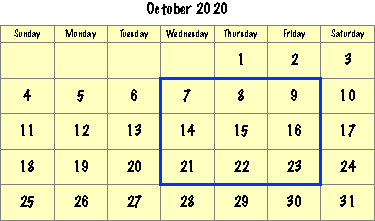
\includegraphics[width=\linewidth]{external/oct-calendar.pdf}
\end{image}%
\tcblower
\end{figureptx}%
Use the example or draw your own 3 by 3 box.%
\item\label{x:task:tsk-oct-b}Find two different patterns among the numbers in the 3 by 3 box. Describe each pattern carefully.%
\item{}Use algebra to justify one of the patterns you found in \hyperref[x:task:tsk-oct-b]{Task~{\xreffont 1.8.2.2}.{\xreffont\ref{x:task:tsk-oct-b}}}. Indicate which pattern you are justifying.%
\end{enumerate}
\end{divisionexercise}%
\begin{divisionexercise}{3}{}{}{g:exercise:idp1872171368}%
A famous pattern called Pascal's Triangle is shown in \hyperref[x:figure:fig-pascal-tri]{Figure~{\xreffont\ref{x:figure:fig-pascal-tri}}}.%
\begin{figureptx}{Pascal's Triangle}{x:figure:fig-pascal-tri}{}%
\begin{image}{0.25}{0.5}{0.25}%
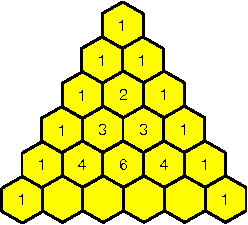
\includegraphics[width=\linewidth]{external/pascal-tri.pdf}
\end{image}%
\tcblower
\end{figureptx}%
\begin{enumerate}[font=\bfseries,label=(\alph*),ref=\alph*]
\item{}Study the pattern. How are the numbers from one row related to the numbers in the next row?%
\item{}Fill-in the missing numbers in the last row. Extend the pattern at least one additional row.%
\item{}Describe 2 patterns that you see in this arrangement of numbers.%
\end{enumerate}
\end{divisionexercise}%
\begin{divisionexercise}{4}{}{}{x:exercise:exer-17-4}%
\begin{enumerate}[font=\bfseries,label=(\alph*),ref=\alph*]
\item{}Using only mental arithmetic, solve each problem in \hyperref[x:table:tbl-17-4]{Table~{\xreffont\ref{x:table:tbl-17-4}}} below. Record how you thought about the numbers to help you add them mentally.%
\begin{tableptx}{\textbf{Table for Exercise~{\xreffont 1.8.2.4}}}{x:table:tbl-17-4}{}%
\centering%
{\tabularfont%
\begin{tabular}{Accl}\hrulethin
\multicolumn{1}{AcA}{\textbf{Simplify}}&\multicolumn{1}{cA}{\textbf{Solution}}&\multicolumn{1}{lA}{\textbf{How did you solve the problem?}}\tabularnewline\hrulethin
\multicolumn{1}{AcA}{\(25 + 26\)}&\multicolumn{1}{cA}{~}&\multicolumn{1}{lA}{~}\tabularnewline\hrulethin
\multicolumn{1}{AcA}{\(15 + 16\)}&\multicolumn{1}{cA}{~}&\multicolumn{1}{lA}{~}\tabularnewline\hrulethin
\multicolumn{1}{AcA}{\(39 + 40\)}&\multicolumn{1}{cA}{~}&\multicolumn{1}{lA}{~}\tabularnewline\hrulethin
\multicolumn{1}{AcA}{\(18 + 19\)}&\multicolumn{1}{cA}{~}&\multicolumn{1}{lA}{~}\tabularnewline\hrulethin
\multicolumn{1}{AcA}{\(25 + 26\)}&\multicolumn{1}{cA}{~}&\multicolumn{1}{lA}{~}\tabularnewline\hrulethin
\multicolumn{1}{AcA}{\(163 + 164\)}&\multicolumn{1}{cA}{~}&\multicolumn{1}{lA}{~}\tabularnewline\hrulethin
\end{tabular}
}%
\end{tableptx}%
\item{}Write the sum \(25 + 26\) in terms of \(x\) with \(x = 25\). Show the sum in terms of \(x\).%
\item{}What other problems did you solve using the same strategy you used to solve \(25 + 26\)? Color code the problems that you solve using the same strategy.%
\item{}Did you use the same strategy to mentally solve all of the problems? If you used more than one strategy, color code problems you solved using the same strategy. Do this for each strategy you used. Describe each strategy.%
\end{enumerate}
\end{divisionexercise}%
\end{exercises-subsection}
\end{sectionptx}
%
%
\typeout{************************************************}
\typeout{Section 1.9 Algebra and Number Puzzles}
\typeout{************************************************}
%
\begin{sectionptx}{Algebra and Number Puzzles}{}{Algebra and Number Puzzles}{}{}{x:section:S_alg_puzz}
%
%
\typeout{************************************************}
\typeout{Subsection 1.9.1 Overview}
\typeout{************************************************}
%
\begin{subsectionptx}{Overview}{}{Overview}{}{}{g:subsection:idp1872191464}
We have made introductions and studied its underlying mathematics. We looked at the order of operations and saw that the order in which we complete operations is purposeful rather than just a convention to memorize. We've experienced finding patterns in the 100s Chart and justifying them with algebra. We've seen mathematics arise in unlikely places. This lesson expands our repertoire of unlikely places for mathematics, magic number puzzles. Could it be that math really is everywhere?%
\par
Throughout human history of the past 2000 years, humans have been fascinated by puzzles. In this lesson, we play with some of them and see how they are related to algebra.%
\end{subsectionptx}
\begin{activity}{}{g:activity:idp1872191848}%
Consider these two magic number puzzles. \begin{assemblage}{Number Puzzle 1.}{g:assemblage:idp1872197096}%
Choose a whole number between 1 and 10.%
\par
Double it.%
\par
Add 4 to the result.%
\par
Divide the result by 2.%
\par
Subtract the number you started with.%
\par
What number to you get?%
\end{assemblage}
%
\par
How does this puzzle work? Act out each step of the puzzle using objects (algebra tiles or blocks and beans will work!) Let one type of object represent \(x\) and another type of object represent units. Finally, solve the puzzle using a variable to represent an unknown number and algebra to write then simplify expressions. \begin{assemblage}{Number Puzzle 2.}{g:assemblage:idp1872194792}%
Choose a number.%
\par
Multiply it by 6.%
\par
Add 12.%
\par
Divide the result by 2.%
\par
Add 9.%
\par
Divide the result by 3.%
\par
What is your number? How does it compare with your starting number?%
\end{assemblage}
 Determine a solution. Figure out how this puzzle works, first with materials, then with algebra.%
\par
Discuss the solutions to both puzzles, including justification with materials and with algebra and the relationship between these.%
\end{activity}%
%
%
\typeout{************************************************}
\typeout{Student Page 1.9.2 Translating Magic Number Puzzles to Algebra to Justify Them}
\typeout{************************************************}
%
\newgeometry{left=1.2in, right=1.2in, top=1in, bottom=1in}
\begin{worksheet-subsection}{Translating Magic Number Puzzles to Algebra to Justify Them}{}{Translating Magic Number Puzzles to Algebra to Justify Them}{}{}{x:worksheet:act-translate-magic}
\begin{introduction}{}%
\hyperref[x:worksheet:act-translate-magic]{Translating Magic Number Puzzles to Algebra to Justify Them} includes several magic number puzzles for you to solve with your group. Follow the directions. Be ready to discuss your solutions with the class.%
\par
Directions: Try each of the Magic Number Puzzles. Figure out how each one works. Write an informal justification for each puzzle. For one of the puzzles, show why it works using algebra.%
\end{introduction}%
\begin{divisionexercise}{1}{}{}{g:exercise:idp1872205160}%
\begin{enumerate}[font=\bfseries,label=(\alph*),ref=\alph*]
\item{}Consider this puzzle:%
\begin{enumerate}[label=(\alph*)]
\item{}Pick a number.%
\item{}Multiply the number by 2.%
\item{}Add 10 to the total.%
\item{}Divide the total by 2.%
\item{}Subtract the first number you chose from the result in the previous step.%
\end{enumerate}
%
\item{}What number do you get? Why?%
\end{enumerate}
\end{divisionexercise}%
\begin{divisionexercise}{2}{}{}{g:exercise:idp1872212456}%
\begin{enumerate}[font=\bfseries,label=(\alph*),ref=\alph*]
\item{}Consider this puzzle:%
\begin{enumerate}[label=(\alph*)]
\item{}Write down your shoe size rounded to a whole number.%
\item{}Multiply the number by 5.%
\item{}Add 50.%
\item{}Multiply the result by 20.%
\item{}Add this year.%
\item{}Subtract 1000.%
\item{}Subtract the year you were born.%
\item{}What is special about the number you get?%
\end{enumerate}
%
\item{}Why does this puzzle work?%
\item{}Does it work for every shoe size? If not, for what shoe sizes do you have to adjust the puzzle to make it work? How do you have to adjust the puzzle?%
\end{enumerate}
\end{divisionexercise}%
\begin{divisionexercise}{3}{}{}{g:exercise:idp1872206696}%
\begin{enumerate}[font=\bfseries,label=(\alph*),ref=\alph*]
\item{}Consider this puzzle:%
\begin{enumerate}[label=(\alph*)]
\item{}Write your age on a slip of paper.%
\item{}Add 90 to your number.%
\item{}Cross out the leftmost digit from the result.%
\item{}Add the digit you crossed off to the result.%
\item{}Add 9 to the result.%
\end{enumerate}
%
\item{}What is the final result? How does it relate to the number you chose?%
\item{}Are there any ages for which this puzzle doesn't work? How do you know?%
\end{enumerate}
\end{divisionexercise}%
\begin{divisionexercise}{4}{}{}{g:exercise:idp1872220904}%
\begin{enumerate}[font=\bfseries,label=(\alph*),ref=\alph*]
\item{}Consider this puzzle:%
\begin{enumerate}[label=(\alph*)]
\item{}Write the year of your birth.%
\item{}Double it.%
\item{}Add 5.%
\item{}Multiply the result by 50.%
\item{}Add your age.%
\item{}Add 365.%
\item{}Subtract 615.%
\end{enumerate}
%
\item{}What is the final result? How does it relate to the numbers you chose in the problem?%
\end{enumerate}
\end{divisionexercise}%
\begin{divisionexercise}{5}{}{}{g:exercise:idp1872222696}%
There were 100 chocolates in a box. The box was passed from person to person in one row. The first person took one chocolate. Each person down the row took one more chocolate than the person before. The box was passed until it was empty. What is the largest number of people that could have removed chocolates from the box? How do you know?%
\end{divisionexercise}%
\begin{divisionexercise}{6}{}{}{g:exercise:idp1872228840}%
Consider this puzzle:%
\begin{enumerate}[label=(\alph*)]
\item{}Choose any number.%
\item{}Multiply the number by 100.%
\item{}Subtract the original number.%
\item{}Add the digits in your answer.%
\end{enumerate}
%
\begin{enumerate}[font=\bfseries,label=(\alph*),ref=\alph*]
\item{}Try the puzzle using single digit numbers (1 through 9). What numbers are possible? How do you know?%
\item{}Try the puzzle using numbers from 10 through 99. What numbers are possible? How do you know?%
\item{}What numbers are possible if you complete the puzzle using 3-digit numbers? Show the numbers you used to get each answer to the final step.%
\item{}One student found that the answer for the final step could be 18, 27, or 36.%
\begin{enumerate}[font=\bfseries,label=(\roman*),ref=\theenumi.\roman*]
\item{}How many digits must the original number have for the puzzle to give 27 as an answer? Find a number that works.%
\item{}How many digits must the original number have for the puzzle to give 36 as an answer? Find a number that works.%
\item{}Are any other numbers possible for the answer to step IV? For any additional step IV solutions you find, show the number you used to get the answer.%
\end{enumerate}
\end{enumerate}
\end{divisionexercise}%
\end{worksheet-subsection}
\restoregeometry
%
%
\typeout{************************************************}
\typeout{Homework 1.9.3 Homework}
\typeout{************************************************}
%
\begin{exercises-subsection}{Homework}{}{Homework}{}{}{g:exercises:idp1872234344}
\begin{divisionexercise}{1}{}{}{g:exercise:idp1872233448}%
Go back to \hyperlink{x:paragraphs:htlmfs-directions}{How To Learn Math For Students Directions}. Complete \hyperref[x:exercise:main-prob-nine]{How to Learn Math for Students Exercise~{\xreffont\ref{x:exercise:main-prob-nine}}}. You will hand in your written reflections for \hyperref[x:exercise:main-prob-nine]{How to Learn Math for Students Exercise~{\xreffont\ref{x:exercise:main-prob-nine}}} in class.%
\end{divisionexercise}%
\begin{divisionexercise}{2}{}{}{g:exercise:idp1872231784}%
Finish solving \hyperref[x:worksheet:act-translate-magic]{Translating Magic Number Puzzles to Algebra to Justify Them} Be ready to discuss solutions and ask any remaining questions in class.%
\end{divisionexercise}%
\begin{divisionexercise}{3}{}{}{g:exercise:idp1872231400}%
National Public Radio regularly congratulates patrons celebrating birthdays and anniversaries. Here's an announcement made in 2017: \begin{quote}%
Congratulations to Laurie on her 24th birthday, counting backwards since 2002.\end{quote}
%
\begin{enumerate}[font=\bfseries,label=(\alph*),ref=\alph*]
\item{}What was Laurie's actual age on the day of the announcement?%
\item{}How old will Laurie be in 2030?%
\item{}How old will Laurie actually be when she says she is 1-year old (assuming she keeps this counting scheme going)? Is she likely to live that long?%
\item{}Write an expression that will help you determine Laurie's NPR age in any year after 2002. Say how you know your expression is correct.%
\end{enumerate}
\end{divisionexercise}%
\begin{divisionexercise}{4}{}{}{g:exercise:idp1872235496}%
Study the following Magic Number Puzzle. Try it out for a few numbers, then show how and why it works using Algebra or pictures.%
\begin{enumerate}[label=(\alph*)]
\item{}Choose a number.%
\item{}Multiply by 6.%
\item{}Add 12.%
\item{}Divide by 2.%
\item{}Subtract 6.%
\item{}Divide by 3.%
\end{enumerate}
%
\begin{enumerate}[font=\bfseries,label=(\alph*),ref=\alph*]
\item{}What is special about the number you get?%
\item{}Why does this puzzle work?%
\end{enumerate}
\end{divisionexercise}%
\begin{divisionexercise}{5}{}{}{g:exercise:idp1872247016}%
Find a magic number puzzle different from those you encountered in this lesson. Write down or print out a puzzle you find. Solve the puzzle and figure out how it works. Be ready to share with your group.%
\end{divisionexercise}%
\end{exercises-subsection}
\end{sectionptx}
\end{chapterptx}
%
%
\typeout{************************************************}
\typeout{Chapter 2 Proportional Reasoning and Linear Functions}
\typeout{************************************************}
%
\begin{chapterptx}{Proportional Reasoning and Linear Functions}{}{Proportional Reasoning and Linear Functions}{}{}{x:chapter:C_lin_funcs}
\begin{introduction}{}%
\hyperref[x:chapter:C_learnmath]{Chapter~{\xreffont\ref{x:chapter:C_learnmath}}} provided many opportunities for you to view mathematics through a variety of contexts in which mathematics arises and through connections among representations. In \hyperref[x:chapter:C_lin_funcs]{Chapter~{\xreffont\ref{x:chapter:C_lin_funcs}}}, you will continue to broaden your exposure to contexts and multiple representations, this time through those that can be modeled by linear functions. To be certain of your facility with linear functions, near the end of the chapter, we include a few functions that are not linear so that you consider more deeply what it means to be linear.%
\begin{activity}{}{g:activity:idp1872239336}%
Before we begin, let's talk about the word, \terminology{function}. We used the word function a few times in \hyperref[x:chapter:C_learnmath]{Chapter~{\xreffont\ref{x:chapter:C_learnmath}}} without defining it. For our purposes, function and equation are almost interchangeable. Equations are more general than functions. Here are some equations:%
\begin{align*}
y \amp = 3x + 4 \amp 2x - 3 \amp = 3x + 4 \amp 8 \amp = 3x + 4\\
y \amp = 5 - 7x \amp 14 - 7x \amp = 5 - 7x \amp 2(3x + 4) \amp = 6x + 8\\
y \amp = 4 \amp x \amp = 11 \amp 1 \amp = - (-1)
\end{align*}
%
\par
Some of the equations above are also functions. Can you guess which equations are also functions? Circle them. Why do you think these are functions and the others are not?%
\par
There are several mathematical definitions of function online. Here are two of them:%
\begin{itemize}[label=\textbullet]
\item{}A function is a special relationship where each input has a single output. (Math is Fun, \href{https://www.mathsisfun.com/definitions/function.html}{online website}\footnotemark{}, retrieved April 16, 2020.)%
\item{}A technical definition of a function is: a \href{http://mathinsight.org/definition/relation}{relation}\footnotemark{} from a set of inputs to a set of possible outputs where each input is related to exactly one output. (Math Insight, \href{http://mathinsight.org/definition/function}{online website}\footnotemark{}, retrieved April 16, 2020.)%
\end{itemize}
Let \(x\) be the variable representing the set of input values. Let \(y\) be the variable representing the set of output values. Use one of these definitions to determine which of the equations above are functions. Be ready to explain your choices.%
\end{activity}%
\footnotetext[9]{\nolinkurl{mathsisfun.com/definitions/function.html}\label{g:fn:idp1872250984}}%
\footnotetext[10]{\nolinkurl{mathinsight.org/definition/relation}\label{g:fn:idp1872253672}}%
\footnotetext[11]{\nolinkurl{mathinsight.org/definition/function}\label{g:fn:idp1872251240}}%
\end{introduction}%
%
%
\typeout{************************************************}
\typeout{Section 2.1 Representations: Graphs, Data, and Algebra through Children's Literature}
\typeout{************************************************}
%
\begin{sectionptx}{Representations: Graphs, Data, and Algebra through Children's Literature}{}{Representations: Graphs, Data, and Algebra through Children's Literature}{}{}{x:section:S_graphs_lit}
\begin{introduction}{}%
Children's literature is a rich source for mathematics connections. Though the stories are intended for children, the underlying mathematics is more advanced. In this lesson, we will read a story and see how it can be represented through graphs, tables, and algebra.%
\end{introduction}%
%
%
\typeout{************************************************}
\typeout{Subsection 2.1.1 Video: Talking About Math}
\typeout{************************************************}
%
\begin{subsectionptx}{Video: Talking About Math}{}{Video: Talking About Math}{}{}{g:subsection:idp1872259432}
In \pubtitle{How to Learn Math for Students}, Lesson 4, watch Video 4: Talking About Math. How can you benefit by actively working in groups both in and outside of class? Think about how well you and your group members currently interact. What ideas do you have about how to help your group work together more productively? Share your ideas with your group.%
\end{subsectionptx}
%
%
\typeout{************************************************}
\typeout{Student Page 2.1.2 The Eyes Have It}
\typeout{************************************************}
%
\newgeometry{left=1.2in, right=1.2in, top=1in, bottom=1in}
\begin{worksheet-subsection}{The Eyes Have It}{}{The Eyes Have It}{}{}{x:worksheet:act-eyes}
\begin{introduction}{}%
Because variables are so important in our work with algebra, it is helpful to further develop our facility with their use. In this activity, you will study the relationship between the numbers of monsters and the corresponding numbers of eyes (each monster has only two eyes) through tables, graphs, English sentences, and algebraic equations.%
\par
Read \pubtitle{Horns to Toes and In Between} by Sandra Boynton. (You can find an \href{https://www.youtube.com/watch?v=5J2BwEu1ueY}{amusing version of the book on YouTube}\footnote{\nolinkurl{youtube.com/watch?v=5J2BwEu1ueY}\label{g:fn:idp1872260840}}.)%
\par
How many eyes do 3 monsters have? 4 monsters? 7 monsters? All the monsters in the book? Any number of monsters (with 2 eyes each)?%
\end{introduction}%
\begin{divisionexercise}{1}{}{}{x:exercise:exer-monsters-1}%
Record the number of eyes based on the number of people in \hyperref[x:table:tbl-monsters]{Table~{\xreffont\ref{x:table:tbl-monsters}}}.%
\begin{tableptx}{\textbf{Monsters\slash{}Eyes Table for Student Page Exercise~{\xreffont 2.1.2.1}}}{x:table:tbl-monsters}{}%
\centering%
{\tabularfont%
\begin{tabular}{Alccccccc}\hrulethin
\multicolumn{1}{AlA}{Number of Monsters, \(M\)}&\multicolumn{1}{cA}{1}&\multicolumn{1}{cA}{2}&\multicolumn{1}{cA}{3}&\multicolumn{1}{cA}{4}&\multicolumn{1}{cA}{5}&\multicolumn{1}{cA}{6}&\multicolumn{1}{cA}{\(M\)}\tabularnewline\hrulethin
\multicolumn{1}{AlA}{Total Number of Eyes, \(E\)}&\multicolumn{1}{cA}{~}&\multicolumn{1}{cA}{~}&\multicolumn{1}{cA}{~}&\multicolumn{1}{cA}{~}&\multicolumn{1}{cA}{~}&\multicolumn{1}{cA}{~}&\multicolumn{1}{cA}{\(E =\)\fillin{4.545454545454546}}\tabularnewline\hrulethin
\end{tabular}
}%
\end{tableptx}%
\end{divisionexercise}%
\begin{divisionexercise}{2}{}{}{x:exercise:exer-monsters-graph}%
Graph the data in \hyperref[x:table:tbl-monsters]{Table~{\xreffont\ref{x:table:tbl-monsters}}} using \hyperref[x:figure:fig-monsters-graph]{Figure~{\xreffont\ref{x:figure:fig-monsters-graph}}}. Label the horizontal axis, Number of Monsters, and the vertical axis, Total Number of Eyes.%
\begin{figureptx}{Blank Graph for Plotting Monsters and Eyes}{x:figure:fig-monsters-graph}{}%
\begin{image}{0.15}{0.7}{0.15}%
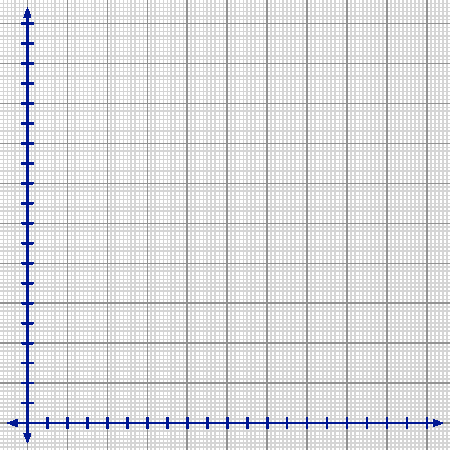
\includegraphics[width=\linewidth]{external/blank-graph.pdf}
\end{image}%
\tcblower
\end{figureptx}%
\begin{enumerate}[font=\bfseries,label=(\alph*),ref=\alph*]
\item{}Starting at 0 where the two axes meet, number the tick marks on the horizontal axis increasing by 1 each time for each dark vertical line (every other tick mark).%
\item{}Choose a reasonable scale for the vertical axis. Explain why the scale is reasonable.%
\item{}Describe the shape of the graph.%
\item{}Why do you think the graph has the shape it does?%
\end{enumerate}
\end{divisionexercise}%
\begin{divisionexercise}{3}{}{}{x:exercise:exer-monsters-relation}%
Describe the relationship between the number of monsters and the total number of eyes the monsters have. Here is one way to phase into the use of variables: \begin{quote}%
The number of \emph{E}yes is two times the number of \emph{M}onsters.%
\par
Number of \emph{E}yes = 2 \texttimes{} number of \emph{M}onsters%
\par
\emph{E} = 2 \texttimes{} \emph{M}%
\par
\emph{E} = 2\emph{M}%
\end{quote}
%
\end{divisionexercise}%
\begin{divisionexercise}{4}{}{}{x:exercise:exer-body-parts}%
Choose a body part that humans have more than 2 of. Repeat \hyperlink{x:exercise:exer-monsters-1}{Student Page Exercise~{\xreffont 2.1.2.1}}, \hyperlink{x:exercise:exer-monsters-graph}{Student Page Exercise~{\xreffont 2.1.2.2}}, and \hyperlink{x:exercise:exer-monsters-relation}{Student Page Exercise~{\xreffont 2.1.2.3}} for the body part you choose. You are welcome to look up numbers on the Internet if you don't know them.%
\end{divisionexercise}%
\begin{divisionexercise}{5}{}{}{g:exercise:idp1872282216}%
Graph number of people versus total number of the chosen body part on the axes above in \hyperref[x:figure:fig-monsters-graph]{Figure~{\xreffont\ref{x:figure:fig-monsters-graph}}}. What do you notice?%
\end{divisionexercise}%
\end{worksheet-subsection}
\restoregeometry
%
%
\typeout{************************************************}
\typeout{Student Page 2.1.3 Graphing with Desmos}
\typeout{************************************************}
%
\newgeometry{left=1.2in, right=1.2in, top=1in, bottom=1in}
\begin{worksheet-subsection}{Graphing with Desmos}{}{Graphing with Desmos}{}{}{x:worksheet:act-desmos}
\begin{introduction}{}%
Read the following instructions. Open Desmos on a computer, a smart phone, or an electronic tablet. Use the directions to plot the data from \hyperref[x:worksheet:act-eyes]{The Eyes Have It}. What questions do you have? Share your graph with your group.%
\end{introduction}%
\begin{divisionexercise}{1}{Desmos.}{}{g:exercise:idp1872287720}%
\begin{enumerate}[font=\bfseries,label=(\alph*),ref=\alph*]
\item{}Google ``Desmos.''%
\item{}Choose Desmos Graphing Calculator.%
\item{}Use with an Internet connection on a computer or download the app onto your smart phone or tablet free of charge.%
\end{enumerate}
\end{divisionexercise}%
\begin{divisionexercise}{2}{Plotting Points with Desmos.}{}{g:exercise:idp1872291048}%
\begin{enumerate}[font=\bfseries,label=(\alph*),ref=\alph*]
\item{}Click on the add item menu, ``+'' (upper left). Choose table.%
\item{}Enter the data from your table into Desmos.%
\item{}Notice that points are being plotting as you type them.%
\item{}You might not be able to see all of your points on the graph.%
\end{enumerate}
\end{divisionexercise}%
\begin{divisionexercise}{3}{Setting the Graphing Window With Desmos.}{}{g:exercise:idp1872291304}%
\begin{enumerate}[font=\bfseries,label=(\alph*),ref=\alph*]
\item{}Click on the wrench icon in the upper right corner.%
\item{}For the independent variable \(x\), enter the low and high values for your data.%
\item{}Choose a reasonable step size. The step is the interval between tick marks on the graph.%
\item{}Include a title for the \(x\)-axis.%
\item{}Repeat for the dependent variable, \(y\).%
\end{enumerate}
\end{divisionexercise}%
\begin{divisionexercise}{4}{Grpahing an Equation.}{}{g:exercise:idp1872300904}%
\begin{enumerate}[font=\bfseries,label=(\alph*),ref=\alph*]
\item{}On the left side of the screen, type in the equation you want to plot in the next entry line.%
\item{}It will automatically appear on the graphing screen.%
\item{}Troubleshoot and change the equation if it doesn't fit the data.%
\end{enumerate}
\end{divisionexercise}%
\end{worksheet-subsection}
\restoregeometry
%
%
\typeout{************************************************}
\typeout{Student Page 2.1.4 The Eyes Have It, Extended}
\typeout{************************************************}
%
\newgeometry{left=1.2in, right=1.2in, top=1in, bottom=1in}
\begin{worksheet-subsection}{The Eyes Have It, Extended}{}{The Eyes Have It, Extended}{}{}{x:worksheet:act-eyes-extend}
\begin{introduction}{}%
What household items do Americans likely have in quantity? Find statistics about the average number of something each household owns. Repeat the activity in \hyperref[x:worksheet:act-eyes]{The Eyes Have It} problems 1 through 3, for the item you are interested in. Create a graph with Desmos to represent the data. Share your work on this problem with your group.%
\end{introduction}%
\begin{divisionexercise}{1}{}{}{g:exercise:idp1872301416}%
How did you decide what scale to use?%
\end{divisionexercise}%
\begin{divisionexercise}{2}{}{}{g:exercise:idp1872296424}%
How did you find the equation to plot?%
\end{divisionexercise}%
\begin{divisionexercise}{3}{}{}{g:exercise:idp1872296296}%
What questions do you have?%
\end{divisionexercise}%
\end{worksheet-subsection}
\restoregeometry
%
%
\typeout{************************************************}
\typeout{Homework 2.1.5 Homework}
\typeout{************************************************}
%
\begin{exercises-subsection}{Homework}{}{Homework}{}{}{g:exercises:idp1872302824}
\begin{divisionexercise}{1}{}{}{g:exercise:idp1872297448}%
Go back to \hyperlink{x:paragraphs:htlmfs-directions}{How To Learn Math For Students Directions}. Complete \hyperref[x:exercise:main-prob-ten]{How to Learn Math for Students Exercise~{\xreffont\ref{x:exercise:main-prob-ten}}}. You will hand in your written reflections for \hyperref[x:exercise:main-prob-ten]{How to Learn Math for Students Exercise~{\xreffont\ref{x:exercise:main-prob-ten}}} in class.%
\end{divisionexercise}%
\begin{divisionexercise}{2}{}{}{x:exercise:desmos-body-parts}%
Revisit \hyperref[x:worksheet:act-eyes]{The Eyes Have It}. Using the data in \hyperlink{x:exercise:exer-body-parts}{Student Page Exercise~{\xreffont 2.1.2.4}} for the Human Body Parts your group chose, create a table listing the number of body parts for 2, 4, 6, 8, and 10 people. Plot the data with Desmos. Choose appropriate scales for both \(x\) and \(y\) if the scales chosen by Desmos do not show all of the data.  Find an equation to fit the data. Print out the graph and data or be prepared to share them electronically.%
\end{divisionexercise}%
\begin{divisionexercise}{3}{}{}{x:exercise:exer-refresh-plotting}%
If plotting points on a coordinate grid is unfamiliar to you, or you need to dust off the skill, return to \hyperlink{x:exercise:desmos-body-parts}{Exercise~{\xreffont 2.1.5.2}}.%
\begin{enumerate}[font=\bfseries,label=(\alph*),ref=\alph*]
\item\label{x:task:exer-refresh-plottinga}Compare the graph with the data in \hyperref[x:table:tbl-example-data]{Table~{\xreffont\ref{x:table:tbl-example-data}}}. Which number is plotted along the horizontal axis? Which number is plotted along the vertical axis?%
\begin{tableptx}{\textbf{Data Table for Exercise~{\xreffont 2.1.5.3}}}{x:table:tbl-example-data}{}%
\centering%
{\tabularfont%
\begin{tabular}{Acc}\hrulethin
\multicolumn{1}{AcA}{\textbf{\(x\)}}&\multicolumn{1}{cA}{\textbf{\(y\)}}\tabularnewline\hrulethin
\multicolumn{1}{AcA}{\(4\)}&\multicolumn{1}{cA}{\(-3\)}\tabularnewline\hrulethin
\multicolumn{1}{AcA}{\(-2\)}&\multicolumn{1}{cA}{\(5\)}\tabularnewline\hrulethin
\multicolumn{1}{AcA}{\(0\)}&\multicolumn{1}{cA}{\(-1\)}\tabularnewline\hrulethin
\multicolumn{1}{AcA}{\(-5\)}&\multicolumn{1}{cA}{\(-4\)}\tabularnewline\hrulethin
\end{tabular}
}%
\end{tableptx}%
\item\label{x:task:exer-refresh-plottingb}Create a new table on Desmos using the values at right. Answer \hyperref[x:task:exer-refresh-plottinga]{Task~{\xreffont 2.1.5.3}.{\xreffont\ref{x:task:exer-refresh-plottinga}}} again.%
\item{}Predict the location of several more points. Enter the points into the table in \hyperref[x:task:exer-refresh-plottingb]{Task~{\xreffont 2.1.5.3}.{\xreffont\ref{x:task:exer-refresh-plottingb}}} to see if you are correct.%
\end{enumerate}
\end{divisionexercise}%
\begin{divisionexercise}{4}{}{}{g:exercise:idp1872320360}%
Movie tickets cost \textdollar{}8.50 each.%
\begin{tableptx}{\textbf{Movie Ticket Data}}{x:table:tbl-tickets}{}%
\centering%
{\tabularfont%
\begin{tabular}{Acc}\hrulethin
\multicolumn{1}{AcA}{\textbf{Number of tickets}}&\multicolumn{1}{cA}{\textbf{Cost of tickets}}\tabularnewline\hrulethin
\multicolumn{1}{AcA}{\(0\)}&\multicolumn{1}{cA}{}\tabularnewline\hrulethin
\multicolumn{1}{AcA}{\(1\)}&\multicolumn{1}{cA}{\(8.50\)}\tabularnewline\hrulethin
\multicolumn{1}{AcA}{\(2\)}&\multicolumn{1}{cA}{}\tabularnewline\hrulethin
\multicolumn{1}{AcA}{\(3\)}&\multicolumn{1}{cA}{}\tabularnewline\hrulethin
\multicolumn{1}{AcA}{\(4\)}&\multicolumn{1}{cA}{}\tabularnewline\hrulethin
\multicolumn{1}{AcA}{\(10\)}&\multicolumn{1}{cA}{}\tabularnewline\hrulethin
\multicolumn{1}{AcA}{\(15\)}&\multicolumn{1}{cA}{}\tabularnewline\hrulethin
\multicolumn{1}{AcA}{\(n\)}&\multicolumn{1}{cA}{}\tabularnewline\hrulethin
\end{tabular}
}%
\end{tableptx}%
\begin{figureptx}{Blank Graph for Movie Tickets}{x:figure:fig-tickets}{}%
\begin{image}{0.25}{0.5}{0.25}%
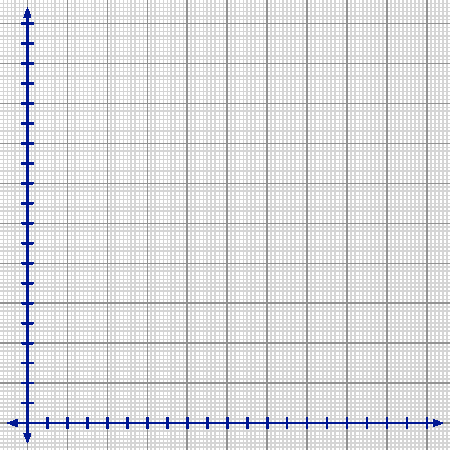
\includegraphics[width=\linewidth]{external/blank-graph.pdf}
\end{image}%
\tcblower
\end{figureptx}%
\begin{enumerate}[font=\bfseries,label=(\alph*),ref=\alph*]
\item{}Complete \hyperref[x:table:tbl-tickets]{Table~{\xreffont\ref{x:table:tbl-tickets}}} to show the cost of the numbers of movie tickets listed if each ticket costs \textdollar{}8.50.%
\item{}Plot the data on the graph at right. Label accurate scales for both \(x\) and \(y\) so that you use most of the graph. Write titles on each axis.%
\item\label{x:task:exer-ticketsc}Describe the relationship between the number of tickets purchased and the cost of that number of tickets.%
\item{}Write the relationship in \hyperref[x:task:exer-ticketsc]{Task~{\xreffont 2.1.5.4}.{\xreffont\ref{x:task:exer-ticketsc}}} as an equation.%
\end{enumerate}
\end{divisionexercise}%
\begin{divisionexercise}{5}{}{}{g:exercise:idp1872331240}%
Gasoline prices sometimes vary greatly in a day. On January 28, 2015, gasoline prices in the Muskegon, MI area ranged from \textdollar{}1.879 to \textdollar{}2.199 per gallon.%
\begin{enumerate}[font=\bfseries,label=(\alph*),ref=\alph*]
\item{}Complete \hyperref[x:table:tbl-gas-prices]{Table~{\xreffont\ref{x:table:tbl-gas-prices}}} to find how much you would pay for the numbers of gallons of gas listed for each gasoline price. Round prices to the nearest penny (hundredth of a dollar).%
\begin{tableptx}{\textbf{Table of Gas Prices}}{x:table:tbl-gas-prices}{}%
\centering%
{\tabularfont%
\begin{tabular}{Accc}\hrulethin
\multicolumn{1}{AcA}{\tablecelllines{c}{m}
{Number of Gallons\\
of Gas Purchased, \(g\)}
}&\multicolumn{2}{cA}{\textbf{Price of Gas, \(P\)}}\tabularnewline\crulethin{2-3}
\multicolumn{1}{AcA}{\textbf{}}&\multicolumn{1}{cA}{\textbf{\textdollar{}1.879 per gallon}}&\multicolumn{1}{cA}{\textbf{\textdollar{}2.199 per gallon}}\tabularnewline\hrulethin
\multicolumn{1}{AcA}{1}&\multicolumn{1}{cA}{}&\multicolumn{1}{cA}{}\tabularnewline\hrulethin
\multicolumn{1}{AcA}{2}&\multicolumn{1}{cA}{}&\multicolumn{1}{cA}{}\tabularnewline\hrulethin
\multicolumn{1}{AcA}{3}&\multicolumn{1}{cA}{}&\multicolumn{1}{cA}{}\tabularnewline\hrulethin
\multicolumn{1}{AcA}{4}&\multicolumn{1}{cA}{}&\multicolumn{1}{cA}{}\tabularnewline\hrulethin
\end{tabular}
}%
\end{tableptx}%
\item{}Accurately plot the data. Label scales and titles for each axis.%
\item{}Write equations in the last row of the table that fit the data. Tell how you know your equations are correct.%
\item{}How many gallons of gasoline can you purchase for \textdollar{}10? Show your work for one of the gasoline prices, accurate to 2 decimal places.%
\end{enumerate}
\end{divisionexercise}%
\end{exercises-subsection}
\end{sectionptx}
%
%
\typeout{************************************************}
\typeout{Section 2.2 Creating and Critiquing Graphs}
\typeout{************************************************}
%
\begin{sectionptx}{Creating and Critiquing Graphs}{}{Creating and Critiquing Graphs}{}{}{x:section:S_create_graphs}
%
%
\typeout{************************************************}
\typeout{Subsection 2.2.1 Overview}
\typeout{************************************************}
%
\begin{subsectionptx}{Overview}{}{Overview}{}{}{g:subsection:idp1872346600}
You have seen that graphs can be helpful in representing data. In Lesson 2.2, you will specifically explore the importance of scale when graphing equations.%
\end{subsectionptx}
%
%
\typeout{************************************************}
\typeout{Student Page 2.2.2 Location, Location, Location}
\typeout{************************************************}
%
\newgeometry{left=1.2in, right=1.2in, top=1in, bottom=1in}
\begin{worksheet-subsection}{Location, Location, Location}{}{Location, Location, Location}{}{}{x:worksheet:act-location}
\begin{introduction}{}%
Through this activity your group will create a graph to convey information about the number of people in a location over time. You will also interpret a graph prepared by another group and try to determine a location that fits the graph. To prepare, think about a place you go with some regularity. How many people are in that place at various times during the day?%
\par
To maximize the interest level, each group must choose very different types of locations. It helps if the numbers of people who go to the place each day are large. Secrecy of choice is critical! Make sure other groups cannot overhear your group's discussions!%
\par
Complete the following with your group:%
\end{introduction}%
\begin{divisionexercise}{1}{}{}{g:exercise:idp1872354920}%
Choose a location and a day of the week to analyze. Get your teacher's approval before continuing (to assure that your group chose a unique location).%
\end{divisionexercise}%
\begin{divisionexercise}{2}{}{}{g:exercise:idp1872355432}%
Estimate how many people are likely to be in the location at the beginning of each hour of the day, starting at 6 AM and ending at 5 AM the following day. Record the data.%
\end{divisionexercise}%
\begin{divisionexercise}{3}{}{}{g:exercise:idp1872355304}%
Create a graph to accurately represent the data.%
\begin{itemize}[label=\textbullet]
\item{}Use the horizontal axis to indicate the hour of the day.%
\item{}Use the vertical axis to indicate the estimated number of people in the location at the beginning of each hour.%
\item{}Do not include any information on your graph that identifies the location your team is analyzing.%
\end{itemize}
%
\par
When you have accomplished the above, your teacher will share your graph with another group and provide another group's graph for your group to analyze.%
\end{divisionexercise}%
\begin{divisionexercise}{4}{}{}{g:exercise:idp1872439272}%
For the new graph:%
\begin{enumerate}[font=\bfseries,label=(\alph*),ref=\alph*]
\item{}Decide what location the graph likely represents.%
\item{}Explain to each other why the graph could represent the location you think it does.%
\item{}Write questions you have about the graph.%
\end{enumerate}
\end{divisionexercise}%
\begin{divisionexercise}{5}{}{}{g:exercise:idp1872438248}%
What features of graphs help you interpret them? What makes these features helpful?%
\end{divisionexercise}%
\begin{divisionexercise}{6}{}{}{g:exercise:idp1872441704}%
Share the graph with the class when asked to do so. Ask questions to help you and others analyze the graph.%
\end{divisionexercise}%
\begin{conclusion}{}%
\hyperref[x:worksheet:act-location]{Location, Location, Location} is adapted from Annenberg Learner, Teaching Math: A Video Library, 5-8, \pubtitle{The Location}, \href{http://www.learner.org/channel/schedule/printmat.html?printmat_id=123}{online website}\footnote{\nolinkurl{learner.org/channel/schedule/printmat.html?printmat_id=123}\label{g:fn:idp1872442984}}, retrieved April 16, 2019.%
\end{conclusion}%
\end{worksheet-subsection}
\restoregeometry
%
%
\typeout{************************************************}
\typeout{Student Page 2.2.3 It's A Matter of Scale}
\typeout{************************************************}
%
\newgeometry{left=1.2in, right=1.2in, top=1in, bottom=1in}
\begin{worksheet-subsection}{It's A Matter of Scale}{}{It's A Matter of Scale}{}{}{x:worksheet:act-scale}
\begin{introduction}{}%
How important are the scales chosen for both the horizontal and vertical axes to the appearance of a graph or a group of graphs? Think about this question as you work together on the following tasks.%
\par
Among groups, compare graphs for \hyperlink{x:exercise:exer-scale-3}{Student Page Exercise~{\xreffont 2.2.3.3}} and \hyperref[x:task:exer-scale-4a]{Task~{\xreffont 2.2.3.4}.{\xreffont\ref{x:task:exer-scale-4a}}}. What do you notice? Think about these questions:%
\begin{itemize}[label=\textbullet]
\item{}Are all of the graphs the same shape?%
\item{}Why did all of the graphs look the same in \hyperlink{x:exercise:exer-scale-3}{Student Page Exercise~{\xreffont 2.2.3.3}}?%
\item{}Why do the graphs look different in \hyperref[x:task:exer-scale-4a]{Task~{\xreffont 2.2.3.4}.{\xreffont\ref{x:task:exer-scale-4a}}}%
\end{itemize}
Discuss the importance of scale.%
\par
Think about \hyperref[x:worksheet:act-location]{Location, Location, Location} How important was scale in helping you determine the location of each place? Does the \(x\)-scale matter? Does the \(y\)-scale matter?%
\par
Directions: Each group member receives a card with an equation on it and both \(x\)- and \(y\)-scales to use to graph the equation. Cards are found in \hyperref[x:worksheet:scale-cards]{It's a Matter of Scale Card Set}.%
\end{introduction}%
\begin{divisionexercise}{1}{}{}{g:exercise:idp1872445160}%
Starting with zero at the origin, the point where the axes intersect, each tick mark increases by the amount of the scale provided. Label both the \(x\)- and \(y\)-axes showing the scale on the card.%
\begin{figureptx}{Blank Graph for \hyperref[x:worksheet:act-scale]{It's A Matter of Scale}}{x:figure:fig-scale-graph}{}%
\begin{image}{0.15}{0.7}{0.15}%
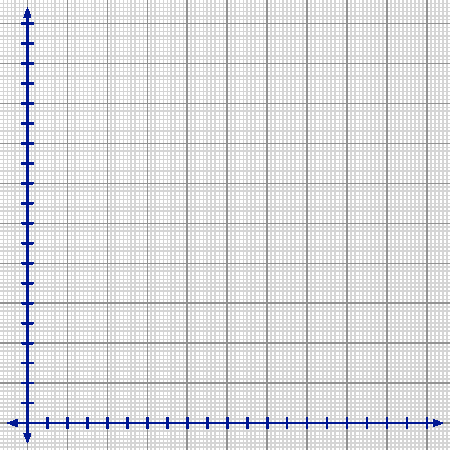
\includegraphics[width=\linewidth]{external/blank-graph.pdf}
\end{image}%
\tcblower
\end{figureptx}%
\end{divisionexercise}%
\begin{divisionexercise}{2}{}{}{x:exercise:exer-scale-2}%
Create a table that fits the equation and \(x\)-scale you were given. Plot the points in the table on the coordinate grid. Graph the equation by connecting the points you found. Write the equation of the line on the graph you drew.%
\end{divisionexercise}%
\begin{divisionexercise}{3}{}{}{x:exercise:exer-scale-3}%
\begin{enumerate}[font=\bfseries,label=(\alph*),ref=\alph*]
\item{}Compare the graphs drawn by members of your group and class. What do you notice?%
\item{}Look carefully at the equations plotted and the scales used. Should the graphs appear as they do? Why or why not?%
\item{}Explain why the graphs appear as they do.%
\end{enumerate}
\end{divisionexercise}%
\begin{divisionexercise}{4}{}{}{g:exercise:idp1872452072}%
Work with other members of your group.%
\begin{figureptx}{New Blank Graph for \hyperref[x:worksheet:act-scale]{It's A Matter of Scale}}{x:figure:fig-scale-graph-repeat}{}%
\begin{image}{0.15}{0.7}{0.15}%
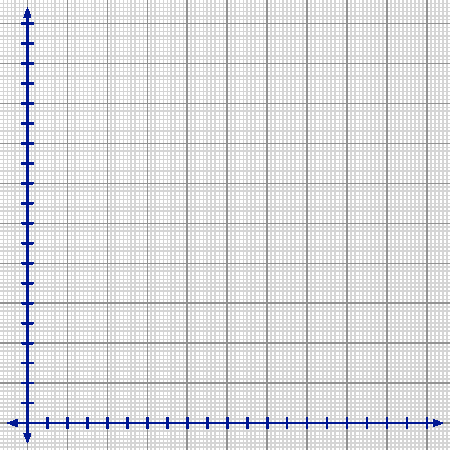
\includegraphics[width=\linewidth]{external/blank-graph.pdf}
\end{image}%
\tcblower
\end{figureptx}%
\begin{enumerate}[font=\bfseries,label=(\alph*),ref=\alph*]
\item\label{x:task:exer-scale-4a}Graph the equations each person was provided on the same graph using the largest \(x\)- and \(y\)-scales provided in the set of cards.%
\item{}What do you notice?%
\item{}Discuss any differences in the appearances of the graphs compared to the graphs plotted in \hyperlink{x:exercise:exer-scale-2}{Student Page Exercise~{\xreffont 2.2.3.2}}.%
\item{}Why do the graphs in \hyperlink{x:exercise:exer-scale-2}{Student Page Exercise~{\xreffont 2.2.3.2}} look different from the graphs in \hyperref[x:task:exer-scale-4a]{Task~{\xreffont 2.2.3.4}.{\xreffont\ref{x:task:exer-scale-4a}}}?%
\end{enumerate}
\end{divisionexercise}%
\begin{divisionexercise}{5}{}{}{g:exercise:idp1872461800}%
Write about the importance of scale in graphing.%
\end{divisionexercise}%
\end{worksheet-subsection}
\restoregeometry
%
%
\typeout{************************************************}
\typeout{Student Page 2.2.4 It's a Matter of Scale Card Set}
\typeout{************************************************}
%
\newgeometry{left=1.2in, right=1.2in, top=1in, bottom=1in}
\begin{worksheet-subsection}{It's a Matter of Scale Card Set}{}{It's a Matter of Scale Card Set}{}{}{x:worksheet:scale-cards}
Directions: Print or copy the following, on separate sheets of paper. Cut the cards apart. Each group member receives one card with all four cards in a row assigned to the same group.%
\begin{image}{0}{1}{0}%
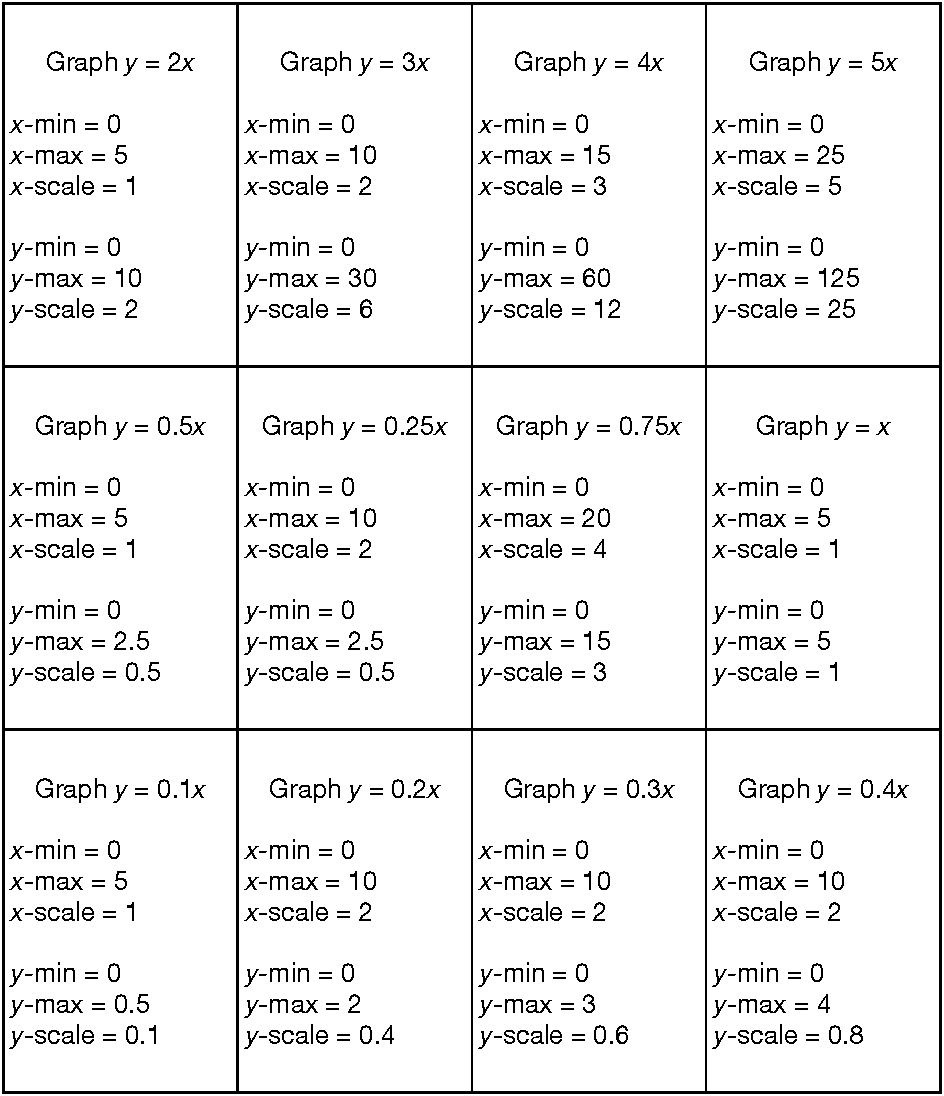
\includegraphics[width=\linewidth]{external/scale-cards-1.pdf}
\end{image}%
\clearpage
Cards continued.%
\begin{image}{0}{1}{0}%
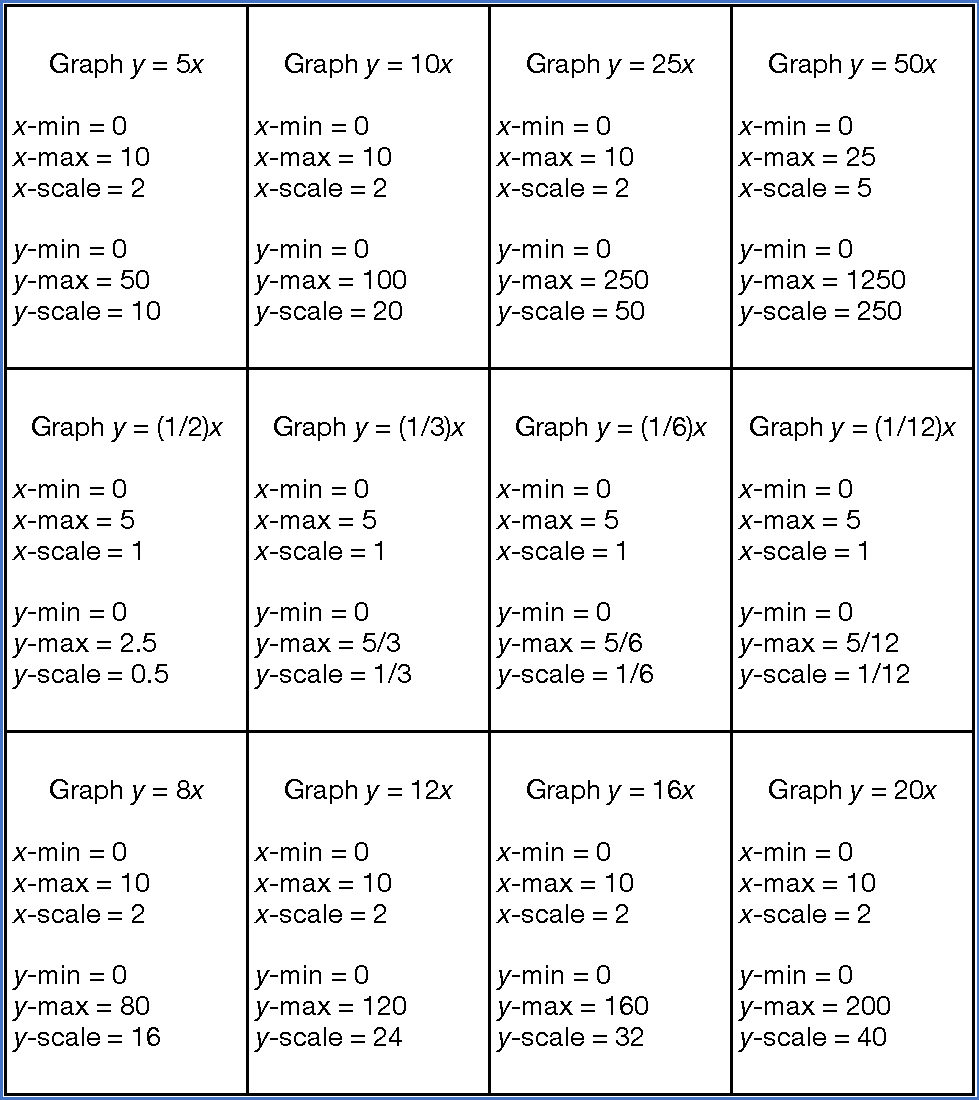
\includegraphics[width=\linewidth]{external/scale-cards-2.pdf}
\end{image}%
\end{worksheet-subsection}
\restoregeometry
%
%
\typeout{************************************************}
\typeout{Student Page 2.2.5 What's Wrong with this Picture? Critiquing Graphs}
\typeout{************************************************}
%
\newgeometry{left=1.2in, right=1.2in, top=1in, bottom=1in}
\begin{worksheet-subsection}{What's Wrong with this Picture? Critiquing Graphs}{}{What's Wrong with this Picture? Critiquing Graphs}{}{}{x:worksheet:act-critique}
\begin{introduction}{}%
News articles and ads are sometimes accompanied by graphs. Sometimes these graphs are deceiving. Complete \hyperref[x:worksheet:act-critique]{What's Wrong with this Picture? Critiquing Graphs}, in light of what you have learned about scale. In each graph check to see if the \(\)- and \(y-\)scales are correct. Are the distances between each of the \(x\)-values to scale?  Are the distances between each of the \(y\)-values to scale? How can you tell?%
\par
Plot each graph using an electronic tool. Set the \(x\) and \(y\) scales to be the same as those used in each graph. Compare the appearance of the graph you created with the designed graph.%
\begin{figureptx}{Graphs for \hyperref[x:worksheet:act-critique]{What's Wrong with this Picture? Critiquing Graphs}}{x:figure:fig-critique-graphs}{}%
\centering
\begin{sidebyside}{2}{0}{0}{0}%
\begin{sbspanel}{0.5}%
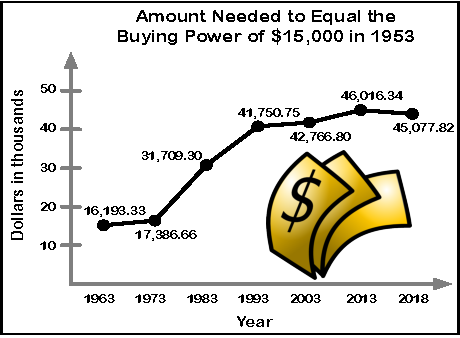
\includegraphics[width=\linewidth]{external/critique-graph1.pdf}
\end{sbspanel}%
\begin{sbspanel}{0.5}%
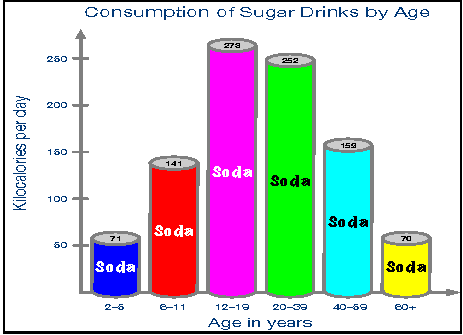
\includegraphics[width=\linewidth]{external/critique-graph2.pdf}
\end{sbspanel}%
\end{sidebyside}%
\begin{sidebyside}{2}{0}{0}{0}%
\begin{sbspanel}{0.5}%
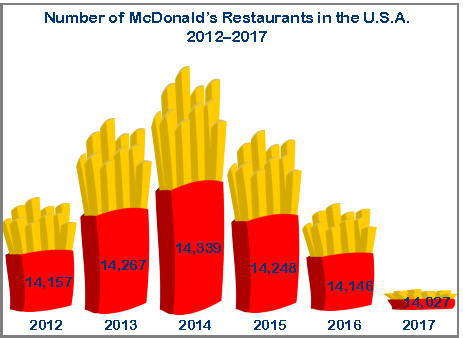
\includegraphics[width=\linewidth]{external/critique-graph3.pdf}
\end{sbspanel}%
\begin{sbspanel}{0.5}%
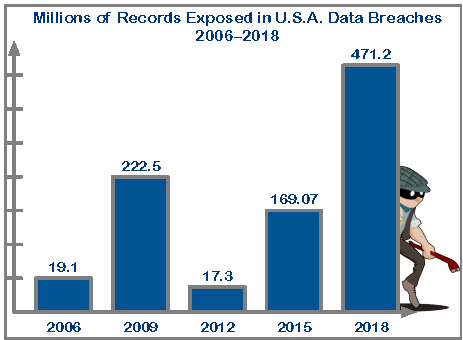
\includegraphics[width=\linewidth]{external/critique-graph4.pdf}
\end{sbspanel}%
\end{sidebyside}%
\tcblower
\end{figureptx}%
\end{introduction}%
\begin{divisionexercise}{1}{}{}{x:exercise:exer-critique-1}%
Study the graphs in \hyperref[x:figure:fig-critique-graphs]{Figure~{\xreffont\ref{x:figure:fig-critique-graphs}}}. Some are accurate, some are not. For each graph:%
\begin{enumerate}[font=\bfseries,label=(\alph*),ref=\alph*]
\item{}Determine if it is drawn accurately. Recreate the graph electronically to help you decide.%
\item{}Which graphs are good representations of the data?%
\item{}Which graphs still need work to make them more accurate? What parts of these graphs need work? Describe any changes needed to help the viewer accurately interpret the information provided.%
\end{enumerate}
\end{divisionexercise}%
\begin{divisionexercise}{2}{}{}{g:exercise:idp1872482664}%
Consider \hyperref[x:table:tbl-traffic-fines]{Table~{\xreffont\ref{x:table:tbl-traffic-fines}}}.%
\begin{sidebyside}{2}{0}{0}{0}%
\begin{sbspanel}{0.5}%
\begin{tableptx}{\textbf{60th District Court Traffic Fines and Costs Schedule}}{x:table:tbl-traffic-fines}{}%
\resizebox{\ifdim\width > \linewidth\linewidth\else\width\fi}{!}{%
{\centering%
{\tabularfont%
\begin{tabular}{Alc}\hrulethin
\multicolumn{1}{AlA}{\textbf{Speeding on Interstate}}&\multicolumn{1}{cA}{\textbf{FINE}}\tabularnewline\hrulethin
\multicolumn{1}{AlA}{71-75 mph}&\multicolumn{1}{cA}{115.00}\tabularnewline\hrulethin
\multicolumn{1}{AlA}{76-80 mph}&\multicolumn{1}{cA}{125.00}\tabularnewline\hrulethin
\multicolumn{1}{AlA}{81-85 mph}&\multicolumn{1}{cA}{135.00}\tabularnewline\hrulethin
\multicolumn{1}{AlA}{86-95 mph}&\multicolumn{1}{cA}{145.00}\tabularnewline\hrulethin
\multicolumn{1}{AlA}{96 mph or above}&\multicolumn{1}{cA}{155.00}\tabularnewline\hrulethin
\end{tabular}
}%
\par}
}%
\end{tableptx}%
\end{sbspanel}%
\begin{sbspanel}{0.5}%
\begin{figureptx}{Blank Graph for \hyperref[x:task:exer-critique-2c]{Task~{\xreffont 2.2.5.2}.{\xreffont\ref{x:task:exer-critique-2c}}}}{x:figure:fig-graph-speeding}{}%
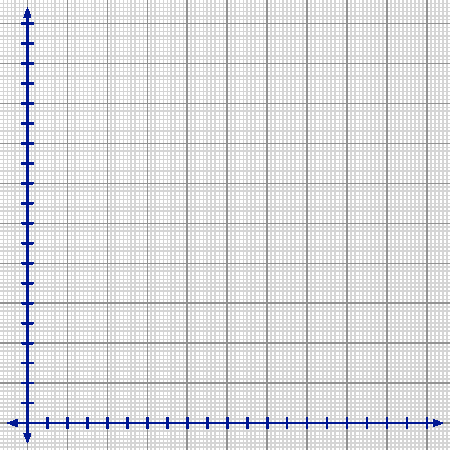
\includegraphics[width=\linewidth]{external/blank-graph.pdf}
\tcblower
\end{figureptx}%
\end{sbspanel}%
\end{sidebyside}%
\begin{enumerate}[font=\bfseries,label=(\alph*),ref=\alph*]
\item{}The independent variable is the variable that changes independent of any other variable. Either you must manipulate this variable yourself, or it changes on its own; it does not rely on the other variable. In the table, what is the independent variable? Why do you think so?%
\item{}The \emph{depend}ent variable is the variable that \emph{depend}s on another variable. What is the dependent variable in the table? Why do you think so?%
\item\label{x:task:exer-critique-2c}Use \hyperref[x:figure:fig-graph-speeding]{Figure~{\xreffont\ref{x:figure:fig-graph-speeding}}} to display the data in \hyperref[x:table:tbl-traffic-fines]{Table~{\xreffont\ref{x:table:tbl-traffic-fines}}}. In mathematics, the horizontal axis \emph{always} represents the independent variable. The vertical axis \emph{always} represents the dependent variable.%
\end{enumerate}
\end{divisionexercise}%
\begin{divisionexercise}{3}{}{}{g:exercise:idp1872499816}%
What are important features of an accurate, informative graph?%
\end{divisionexercise}%
\begin{divisionexercise}{4}{}{}{g:exercise:idp1872494696}%
Read a \href{http://www.huffingtonpost.com/raviparikh/lie-with-data-visualization_b_5169715.html}{data analytics co-founder's point of view of how graphs can distort the facts}\footnotemark{}, retrieved April 21, 2020.%
\begin{enumerate}[font=\bfseries,label=(\alph*),ref=\alph*]
\item{}The author indicates three of the most common ways graphs can be designed to cause data to be misleading. Are any of these ways used to create misleading graphs in \hyperlink{x:exercise:exer-critique-1}{Student Page Exercise~{\xreffont 2.2.5.1}}.%
\item{}Find or create a graph (if you create the graph use real data) that misleads the public. Explain what is misleading about the graph.%
\end{enumerate}
\end{divisionexercise}%
\footnotetext[14]{\nolinkurl{huffingtonpost.com/raviparikh/lie-with-data-visualization_b_5169715.html}\label{g:fn:idp1872493160}}%
\begin{conclusion}{}%
Data sources for graphs, retrieved April 20, 2020:%
\begin{itemize}[label=\textbullet]
\item{}\href{https://www.in2013dollars.com/New-cars/price-inflation}{Amount Needed to Equal the Buying Power of \textdollar{}15,000 in 1953}\footnote{\nolinkurl{in2013dollars.com/New-cars/price-inflation}\label{g:fn:idp1872498024}}.%
\item{}Consumption of Sugar Drinks by Age: U.S. Department of Health and Human Services, Centers for Disease Control and Prevention, National Center for Health Statistics, NCHS Data Brief No. 71, August 2011.%
\item{}\href{https://www.statista.com/statistics/256040/mcdonalds-restaurants-in-north-america/}{Number of McDonald's Restaurants in the U.S.A.}\footnote{\nolinkurl{statista.com/statistics/256040/mcdonalds-restaurants-in-north-america/}\label{g:fn:idp1872495976}}%
\item{}\href{https://www.statista.com/statistics/273550/data-breaches-recorded-in-the-united-states-by-number-of-breaches-and-records-exposed/}{Millions of Records Exposed in U.S.A. Data Breaches}\footnote{\nolinkurl{statista.com/statistics/273550/data-breaches-recorded-in-the-united-states-by-number-of-breaches-and-records-exposed/}\label{g:fn:idp1872498536}}.%
\end{itemize}
%
\end{conclusion}%
\end{worksheet-subsection}
\restoregeometry
%
%
\typeout{************************************************}
\typeout{Subsection 2.2.6 Important Features of Graphs}
\typeout{************************************************}
%
\begin{subsectionptx}{Important Features of Graphs}{}{Important Features of Graphs}{}{}{g:subsection:idp1872506856}
Through \hyperref[x:worksheet:act-critique]{What's Wrong with this Picture? Critiquing Graphs}, you had the opportunity to determine important features of accurate, informative graphs. Your list should include:%
\begin{paragraphs}{The Origin.}{g:paragraphs:idp1872509160}%
Both the \(x\)- and \(y\)-axes must include zero. The intersection of the two axes is called the origin. It represents \((0, 0)\), the place where both \(x\) and \(y\) are zero.%
\end{paragraphs}%
\begin{paragraphs}{Scale.}{g:paragraphs:idp1872506728}%
The distance between consecutive tick marks must represent the same distance as the distance between 0 and the first tick mark. The \(x\)-scale can be different from the \(y\)-scale. Use as much of the graph as possible while still using a scale that is easy to interpret.%
\end{paragraphs}%
\begin{paragraphs}{Plotting Points.}{g:paragraphs:idp1872504168}%
Once the scale is chosen, the data points must be plotted accurately. Each point has 2 coordinates, \((x, y)\), where \(x\) represents a value of the independent variable and \(y\) represents the corresponding value of the dependent variable. If the scales for \(x\) and \(y\) are chosen so that they are easy to interpret, it is likely the points will be relatively easy to locate and plot.%
\end{paragraphs}%
\begin{paragraphs}{Labels.}{g:paragraphs:idp1872513640}%
Label both axes with the quantities they represent. The \(x\)-axis (horizontal) represents the independent variable. The \(y\)-axis (vertical) represents the dependent variable.%
\end{paragraphs}%
\begin{paragraphs}{Title.}{g:paragraphs:idp1872516712}%
In formal documents, a title is necessary. For our purposes, a title on the graph is required when the graph represents data given in context.%
\end{paragraphs}%
\end{subsectionptx}
%
%
\typeout{************************************************}
\typeout{Homework 2.2.7 Homework}
\typeout{************************************************}
%
\begin{exercises-subsection}{Homework}{}{Homework}{}{}{x:exercises:hmwk-create-graphs}
\begin{divisionexercise}{1}{}{}{g:exercise:idp1872515560}%
Optional. Go back to \hyperlink{x:paragraphs:htlmfs-directions}{How To Learn Math For Students Directions}. Complete \hyperref[x:exercise:main-prob-eleven]{How to Learn Math for Students Exercise~{\xreffont\ref{x:exercise:main-prob-eleven}}}. Completing the course helps you develop and build a growth mindset in mathematics. Keep the ideas you have learned from \pubtitle{How to Learn Math for Students} in mind as you complete \pubtitle{Beginning Algebra Made Useful} and any future courses you take in mathematics. Hand in your earned certificate of completion in class to earn privileges as designated by your professor for completing the course.%
\end{divisionexercise}%
\begin{divisionexercise}{2}{}{}{x:exercise:exer-walking-22}%
One mile equals 2000 average steps while walking. If you walk at a rate of 3 miles per hour, you will average 100 steps per minute. \footnotemark{}%
\begin{enumerate}[font=\bfseries,label=(\alph*),ref=\alph*]
\item\label{x:task:exer22-2a}Complete \hyperref[x:table:tbl-steps]{Table~{\xreffont\ref{x:table:tbl-steps}}}.%
\begin{tableptx}{\textbf{Table for Task~{\xreffont 2.2.7.2}.{\xreffont\ref*{x:task:exer22-2a}}}}{x:table:tbl-steps}{}%
\centering%
{\tabularfont%
\begin{tabular}{Acc}\hrulethin
\multicolumn{1}{AcA}{\textbf{Number of minutes}}&\multicolumn{1}{cA}{\textbf{Number of steps taken}}\tabularnewline\hrulethin
\multicolumn{1}{AcA}{1}&\multicolumn{1}{cA}{100}\tabularnewline\hrulethin
\multicolumn{1}{AcA}{10}&\multicolumn{1}{cA}{}\tabularnewline\hrulethin
\multicolumn{1}{AcA}{20}&\multicolumn{1}{cA}{}\tabularnewline\hrulethin
\multicolumn{1}{AcA}{30}&\multicolumn{1}{cA}{}\tabularnewline\hrulethin
\multicolumn{1}{AcA}{40}&\multicolumn{1}{cA}{}\tabularnewline\hrulethin
\end{tabular}
}%
\end{tableptx}%
\item{}Plot the number of minutes versus the number of steps taken. Indicate the scales and titles for each axis.%
\end{enumerate}
\end{divisionexercise}%
\footnotetext[18]{\href{https://www.verywellfit.com/pedometer-step-equivalents-for-exercises-and-activities-3435742}{Resource}\footnotemark{}, retrieved April 21, 2020\label{g:fn:idp1872511208}}%
\footnotetext[19]{\nolinkurl{verywellfit.com/pedometer-step-equivalents-for-exercises-and-activities-3435742}\label{g:fn:idp1872512360}}%
\begin{divisionexercise}{3}{}{}{x:exercise:exer-wages-22}%
As of January 1, 2020, the minimum wage for non-tipped employees in Michigan is \textdollar{}9.65 per hour. How much will you earn if you work \(h\) hours? \footnotemark{}%
\begin{enumerate}[font=\bfseries,label=(\alph*),ref=\alph*]
\item\label{x:task:exer22-3a}Complete \hyperref[x:table:tbl-wages]{Table~{\xreffont\ref{x:table:tbl-wages}}}.%
\begin{tableptx}{\textbf{Table for Task~{\xreffont 2.2.7.3}.{\xreffont\ref*{x:task:exer22-3a}}}}{x:table:tbl-wages}{}%
\centering%
{\tabularfont%
\begin{tabular}{Acc}\hrulethin
\multicolumn{1}{AcA}{\textbf{Hours worked}}&\multicolumn{1}{cA}{\textbf{Amount earned}}\tabularnewline\hrulethin
\multicolumn{1}{AcA}{1}&\multicolumn{1}{cA}{}\tabularnewline\hrulethin
\multicolumn{1}{AcA}{10}&\multicolumn{1}{cA}{}\tabularnewline\hrulethin
\multicolumn{1}{AcA}{20}&\multicolumn{1}{cA}{}\tabularnewline\hrulethin
\multicolumn{1}{AcA}{30}&\multicolumn{1}{cA}{}\tabularnewline\hrulethin
\multicolumn{1}{AcA}{40}&\multicolumn{1}{cA}{}\tabularnewline\hrulethin
\end{tabular}
}%
\end{tableptx}%
\item{}Plot the number of hours worked versus the amount earned. Indicate the scales and titles for each axis.%
\item{}Choose another state from \href{https://www.paycor.com/resource-center/minimum-wage-by-state}{the website the data were found}\footnotemark{}. Complete a table and graph the data for the state you chose.%
\end{enumerate}
\end{divisionexercise}%
\footnotetext[20]{\href{https://www.paycor.com/resource-center/minimum-wage-by-state}{Resource}\footnotemark{}, retrieved April 21, 2020\label{g:fn:idp1872528488}}%
\footnotetext[21]{\nolinkurl{paycor.com/resource-center/minimum-wage-by-state}\label{g:fn:idp1872528232}}%
\footnotetext[22]{\nolinkurl{paycor.com/resource-center/minimum-wage-by-state}\label{g:fn:idp1872541544}}%
\begin{divisionexercise}{4}{}{}{g:exercise:idp1872535656}%
The graph in \hyperref[x:figure:fig-fuel-eff]{Figure~{\xreffont\ref{x:figure:fig-fuel-eff}}} indicates the average fuel efficiency in miles per gallon for a new car in the year shown. (Resource: \href{https://www.bts.gov/content/average-fuel-efficiency-us-passenger-cars-and-light-trucks}{Bureau of Transportation Statistics}\footnotemark{}, retrieved 4\slash{}21\slash{}20.))%
\begin{figureptx}{Average Fuel Efficiency of U.S. Passenger Cars}{x:figure:fig-fuel-eff}{}%
\begin{image}{0.15}{0.7}{0.15}%
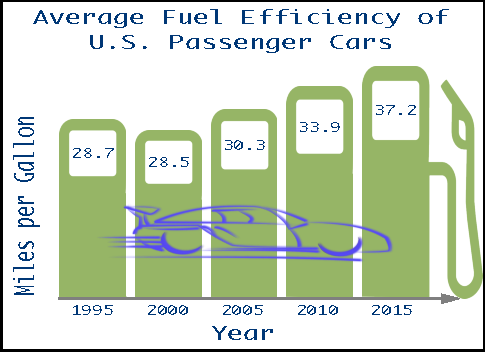
\includegraphics[width=\linewidth]{external/fuel-eff.pdf}
\end{image}%
\tcblower
\end{figureptx}%
\begin{enumerate}[font=\bfseries,label=(\alph*),ref=\alph*]
\item\label{x:task:exer-fuel-a}Complete \hyperref[x:table:tbl-fuel-eff]{Table~{\xreffont\ref{x:table:tbl-fuel-eff}}} for the data in \hyperref[x:figure:fig-fuel-eff]{Figure~{\xreffont\ref{x:figure:fig-fuel-eff}}}.%
\begin{tableptx}{\textbf{Data of Fuel Efficiency of U.S. Passenger Carse}}{x:table:tbl-fuel-eff}{}%
\centering%
{\tabularfont%
\begin{tabular}{Accc}\hrulethin
\multicolumn{1}{AcA}{\textbf{Year}}&\multicolumn{1}{cA}{\textbf{Adjusted year, \(x\)}}&\multicolumn{1}{cA}{\textbf{Fuel efficiency in mpg}}\tabularnewline\hrulethin
\multicolumn{1}{AcA}{1995}&\multicolumn{1}{cA}{0}&\multicolumn{1}{cA}{~}\tabularnewline\hrulethin
\multicolumn{1}{AcA}{2000}&\multicolumn{1}{cA}{5}&\multicolumn{1}{cA}{~}\tabularnewline\hrulethin
\multicolumn{1}{AcA}{2005}&\multicolumn{1}{cA}{}&\multicolumn{1}{cA}{~}\tabularnewline\hrulethin
\multicolumn{1}{AcA}{2010}&\multicolumn{1}{cA}{}&\multicolumn{1}{cA}{~}\tabularnewline\hrulethin
\multicolumn{1}{AcA}{2015}&\multicolumn{1}{cA}{}&\multicolumn{1}{cA}{~}\tabularnewline\hrulethin
\end{tabular}
}%
\end{tableptx}%
\item{}Plot the data, Adjusted Year versus Average Fuel Efficiency.%
\item{}Is the graph accurate for the set of data you listed in \hyperref[x:task:exer-fuel-a]{Task~{\xreffont 2.2.7.4}.{\xreffont\ref{x:task:exer-fuel-a}}}? Why or why not? Discuss both \(x\) and \(y\)-scales and other pertinent aspects of accurate graphs.%
\end{enumerate}
\end{divisionexercise}%
\footnotetext[23]{\nolinkurl{bts.gov/content/average-fuel-efficiency-us-passenger-cars-and-light-trucks}\label{g:fn:idp1872534632}}%
\begin{divisionexercise}{5}{}{}{g:exercise:idp1872557288}%
Study \hyperref[x:figure:fig-life-expect]{Figure~{\xreffont\ref{x:figure:fig-life-expect}}}. Life expectancy at birth indicates the number of years a newborn would live if prevailing patterns of mortality at the time of birth stay the same throughout life.%
\begin{figureptx}{Years of Life Expectancy at Birth}{x:figure:fig-life-expect}{}%
\begin{image}{0.25}{0.5}{0.25}%
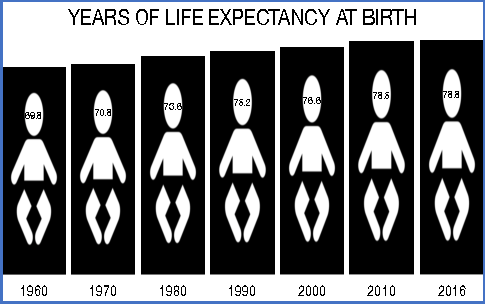
\includegraphics[width=\linewidth]{external/life-expect.pdf}
\end{image}%
\tcblower
\end{figureptx}%
\begin{enumerate}[font=\bfseries,label=(\alph*),ref=\alph*]
\item\label{x:task:exer-life-a}Create a table for the data in the figure. Year is the independent variable.%
\item{}Adjust the values for the independent variable so 1960 is year 0.%
\item{}Plot the data, adjusted year vs. Years of life expectancy at birth.%
\item{}Is the figure accurate for the set of data you listed in \hyperref[x:task:exer-life-a]{Task~{\xreffont 2.2.7.5}.{\xreffont\ref{x:task:exer-life-a}}}? Why or why not?%
\end{enumerate}
\end{divisionexercise}%
\begin{divisionexercise}{6}{}{}{g:exercise:idp1872550248}%
Find more graphs to analyze in print or online news sources. Find at least one graph that is complete and accurate. Find at least one graph that is misleading. In both cases, state briefly how you know the graph is accurate or how you know the graph is misleading.%
\end{divisionexercise}%
\end{exercises-subsection}
\end{sectionptx}
%
%
\typeout{************************************************}
\typeout{Section 2.3 Interpreting and Creating Graphs: The Hare and the Tortoise}
\typeout{************************************************}
%
\begin{sectionptx}{Interpreting and Creating Graphs: The Hare and the Tortoise}{}{Interpreting and Creating Graphs: The Hare and the Tortoise}{}{}{x:section:S_interpret_graphs}
%
%
\typeout{************************************************}
\typeout{Subsection 2.3.1 Overview}
\typeout{************************************************}
%
\begin{subsectionptx}{Overview}{}{Overview}{}{}{g:subsection:idp1872566248}
This section explores graphs in more detail, specifically how to interpret and create graphs. We will explore the common tale of the Hare and the Tortoise for this purpose.%
\end{subsectionptx}
%
%
\typeout{************************************************}
\typeout{Student Page 2.3.2 Can You Walk These Graphs?}
\typeout{************************************************}
%
\newgeometry{left=1.2in, right=1.2in, top=1in, bottom=1in}
\begin{worksheet-subsection}{Can You Walk These Graphs?}{}{Can You Walk These Graphs?}{}{}{x:worksheet:act-walk-graphs}
\begin{introduction}{}%
Use a Calculator-Based Ranger (\initialism{CBR}) connected to a graphing calculator to walk the graphs shown on the student page. For each graph, decide how you will move before you walk. If the graph created by the \initialism{CBR} does not match the graph on the student page, think more carefully about what movement the graph represents. Revise your walk to recreate the graph. What does the \(x\)-axis represent in terms of your movement? What does the \(y\)-axis represent in terms of your movement? How do you know?%
\end{introduction}%
\begin{divisionexercise}{1}{}{}{g:exercise:idp1872565608}%
Use a graphing calculator and a \initialism{CBR} walk to create these graphs. How do you need to move to create each graph?%
\begin{enumerate}[font=\bfseries,label=(\alph*),ref=\alph*]
\item{}\begin{image}{0.325}{0.35}{0.325}%
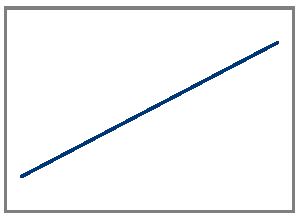
\includegraphics[width=\linewidth]{external/walk-graphs-1.pdf}
\end{image}%
%
\item{}\begin{image}{0.325}{0.35}{0.325}%
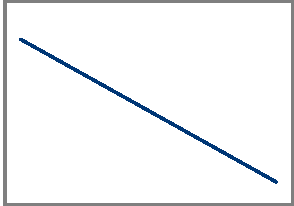
\includegraphics[width=\linewidth]{external/walk-graphs-2.pdf}
\end{image}%
%
\item{}\begin{image}{0.325}{0.35}{0.325}%
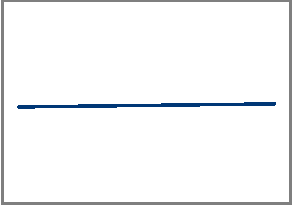
\includegraphics[width=\linewidth]{external/walk-graphs-3.pdf}
\end{image}%
%
\item{}\begin{image}{0.325}{0.35}{0.325}%
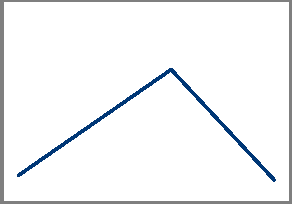
\includegraphics[width=\linewidth]{external/walk-graphs-4.pdf}
\end{image}%
%
\item{}\begin{image}{0.325}{0.35}{0.325}%

\includegraphics[width=\linewidth]{external/walk-graphs-5.pdf}
\end{image}%
%
\item{}\begin{image}{0.325}{0.35}{0.325}%
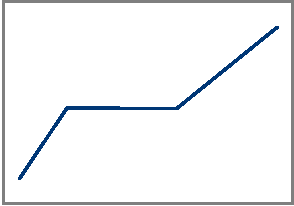
\includegraphics[width=\linewidth]{external/walk-graphs-6.pdf}
\end{image}%
%
\item{}\begin{image}{0.325}{0.35}{0.325}%
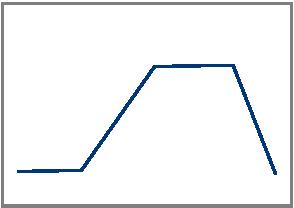
\includegraphics[width=\linewidth]{external/walk-graphs-7.pdf}
\end{image}%
%
\item{}\begin{image}{0.325}{0.35}{0.325}%
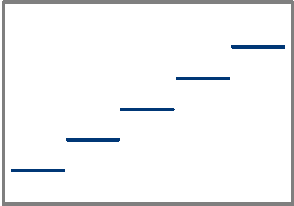
\includegraphics[width=\linewidth]{external/walk-graphs-8.pdf}
\end{image}%
%
\end{enumerate}
\end{divisionexercise}%
\begin{divisionexercise}{2}{}{}{g:exercise:idp1872567144}%
\begin{enumerate}[font=\bfseries,label=(\alph*),ref=\alph*]
\item{}What does the \(x\)-axis represent? Why do you think so?%
\item{}What does the \(y\)-axis represent? Why do you think so?%
\item{}Challenge each other by creating other graphs to match. Also try to walk some of the graphs in the Distance Match application in the Easy Data program for the \initialism{CBR}.%
\end{enumerate}
\end{divisionexercise}%
\end{worksheet-subsection}
\restoregeometry
%
%
\typeout{************************************************}
\typeout{Student Page 2.3.3 The Hare and the Tortoise}
\typeout{************************************************}
%
\newgeometry{left=1.2in, right=1.2in, top=1in, bottom=1in}
\begin{worksheet-subsection}{The Hare and the Tortoise}{}{The Hare and the Tortoise}{}{}{x:worksheet:act-hare-tort}
\begin{introduction}{}%
\pubtitle{The Hare and the Tortoise} extends the work you began in \hyperref[x:worksheet:act-walk-graphs]{Can You Walk These Graphs?} Now consider a race between two unlikely contestants. You will draw a graph to represent each contestant's movement and explain how you know each graph is correct. You will also analyze and interpret additional graphs of the Hare's performance in subsequent races. Finally, you will create your own graph and story to accompany it.%
\par
Taken together, these activities, \hyperref[x:worksheet:act-walk-graphs]{Can You Walk These Graphs?} and \hyperref[x:worksheet:act-hare-tort]{The Hare and the Tortoise}, help you bring your extensive familiarity with traveling from one place to another to bear on your learning first about graphs and then about linear functions. \begin{quote}%
A hare one day ridiculed the short feet and slow pace of the tortoise. The latter, laughing, said, ``Though you be swift as the wind, I will beat you in a race.'' The hare, deeming her assertion to be simply impossible, assented to the proposal; and they agreed that the fox should choose the course, and fix the goal. On the day appointed for the race they started together. The tortoise never for a moment stopped, but went on with a slow but steady pace straight to the end of the course. The hare, trusting to his native swiftness, cared little about the race, and lying down by the wayside, fell fast asleep. At last waking up, and moving as fast as he could, he saw the tortoise had reached the goal, and was comfortably dozing after her fatigue. \footnote{(\href{http://www.pitt.edu/\~dash/type0275.html\#townsend}{Source}\footnote{\nolinkurl{pitt.edu/\~dash/type0275.html\#townsend}\label{g:fn:idp1872582120}}. Retrieved July 27, 2016.)\label{g:fn:idp1872581608}}%
\nopagebreak\par%
\hfill\textemdash{}{\setlength{\tabcolsep}{0pt}\begin{tabular}[t]{l@{}}
Aesop (translated by George Fyler Townsend)
\end{tabular}}\\\par
\end{quote}
%
\end{introduction}%
\begin{divisionexercise}{1}{}{}{g:exercise:idp1872586856}%
\begin{enumerate}[font=\bfseries,label=(\alph*),ref=\alph*]
\item{}On the coordinate grid in \hyperref[x:figure:fig-hare-grid]{Figure~{\xreffont\ref{x:figure:fig-hare-grid}}}, draw a graph to illustrate the tortoise's distance from the starting line over the time it took her to complete the race.%
\begin{figureptx}{Coordinate Grid for \hyperref[x:worksheet:act-hare-tort]{The Hare and the Tortoise}}{x:figure:fig-hare-grid}{}%
\begin{image}{0.15}{0.7}{0.15}%
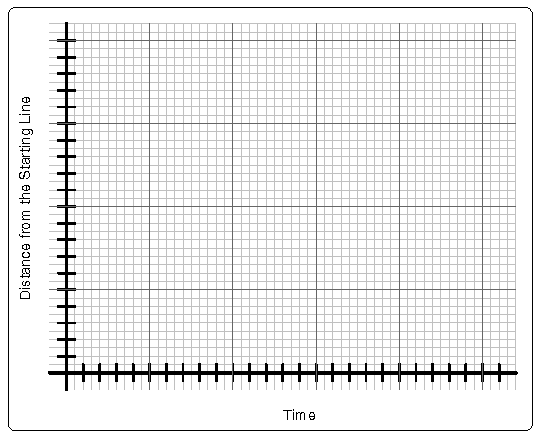
\includegraphics[width=\linewidth]{external/hare-grid.pdf}
\end{image}%
\tcblower
\end{figureptx}%
\item{}On the same grid in \hyperref[x:figure:fig-hare-grid]{Figure~{\xreffont\ref{x:figure:fig-hare-grid}}}, draw a graph to illustrate the hare's distance from the starting line over the time it took him to complete the race.%
\item{}Explain how you know each graph fits the story.%
\end{enumerate}
\end{divisionexercise}%
\begin{divisionexercise}{2}{}{}{g:exercise:idp1872589544}%
Study \hyperref[x:figure:fig-hare-graph-1]{Figure~{\xreffont\ref{x:figure:fig-hare-graph-1}}}, \hyperref[x:figure:fig-hare-graph-2]{Figure~{\xreffont\ref{x:figure:fig-hare-graph-2}}}, \hyperref[x:figure:fig-hare-graph-3]{Figure~{\xreffont\ref{x:figure:fig-hare-graph-3}}}, and \hyperref[x:figure:fig-hare-graph-4]{Figure~{\xreffont\ref{x:figure:fig-hare-graph-4}}}. Each graph shows the hare's movement in subsequent races.%
\begin{sidebyside}{2}{0}{0}{0}%
\begin{sbspanel}{0.5}%
\begin{figureptx}{Hare Movement: Graph A}{x:figure:fig-hare-graph-1}{}%
\includegraphics[width=\linewidth]{external/hare-graph-1.pdf}
\tcblower
\end{figureptx}%
\end{sbspanel}%
\begin{sbspanel}{0.5}%
\begin{figureptx}{Hare Movement: Graph B}{x:figure:fig-hare-graph-2}{}%
\includegraphics[width=\linewidth]{external/hare-graph-2.pdf}
\tcblower
\end{figureptx}%
\end{sbspanel}%
\end{sidebyside}%
\begin{sidebyside}{2}{0}{0}{0}%
\begin{sbspanel}{0.5}%
\begin{figureptx}{Hare Movement: Graph C}{x:figure:fig-hare-graph-3}{}%
\includegraphics[width=\linewidth]{external/hare-graph-3.pdf}
\tcblower
\end{figureptx}%
\end{sbspanel}%
\begin{sbspanel}{0.5}%
\begin{figureptx}{Hare Movement: Graph D}{x:figure:fig-hare-graph-4}{}%
\includegraphics[width=\linewidth]{external/hare-graph-4.pdf}
\tcblower
\end{figureptx}%
\end{sbspanel}%
\end{sidebyside}%
\begin{enumerate}[font=\bfseries,label=(\alph*),ref=\alph*]
\item{}Where on the axes would it make sense to mark the starting line set by the fox?%
\item{}Where on the axes would it make sense to mark the finish line set by the fox?%
\item{}Write a story to go with each race. Describe specifically how the hare is moving:%
\begin{itemize}[label=\textbullet]
\item{}Where does the hare start the race? Finish the race?%
\item{}At what time does the hare start the race? Finish the race?%
\item{}How fast is the hare moving on each tiem interval compared to his speed on the other time intervals?%
\item{}What direction is the hare moving?%
\item{}How do the start and finish times and locations compare from race to race?%
\end{itemize}
%
\end{enumerate}
\end{divisionexercise}%
\begin{divisionexercise}{3}{}{}{g:exercise:idp1872591720}%
Write your own travel story. Draw a graph using \hyperref[x:figure:fig-hare-repeat]{Figure~{\xreffont\ref{x:figure:fig-hare-repeat}}} to illustrate the characters' distance from a starting location at each time during their travels.%
\begin{figureptx}{Blank Graph for Your Own Travel Story}{x:figure:fig-hare-repeat}{}%
\begin{image}{0.15}{0.7}{0.15}%
\includegraphics[width=\linewidth]{external/hare-grid.pdf}
\end{image}%
\tcblower
\end{figureptx}%
\end{divisionexercise}%
\begin{divisionexercise}{4}{}{}{g:exercise:idp1872606056}%
Reflections:%
\begin{enumerate}[font=\bfseries,label=(\alph*),ref=\alph*]
\item{}What clues do you look for in a travel story to help you create a graph to model the time and travel?%
\item{}What clues do you look for in a graph to help you interpret the graph in terms of time and travel?%
\end{enumerate}
\end{divisionexercise}%
\end{worksheet-subsection}
\restoregeometry
%
%
\typeout{************************************************}
\typeout{Homework 2.3.4 Homework}
\typeout{************************************************}
%
\begin{exercises-subsection}{Homework}{}{Homework}{}{}{g:exercises:idp1872606568}
\begin{divisionexercise}{1}{}{}{g:exercise:idp1872599656}%
To get a motion detector to generate the graphs below, how would you have to walk? Describe where the motion detector is located, your relative speed over each section of the graph, how you must walk so that the corners appear, etc. Label points (a, b, c, d, etc.) on the \(x\)-axis to help the reader interpret your description of your walk over each time interval.%
\begin{enumerate}[font=\bfseries,label=(\alph*),ref=\alph*]
\item{}\begin{image}{0.25}{0.5}{0.25}%
\includegraphics[width=\linewidth]{external/exer-walk-graphs-1.pdf}
\end{image}%
%
\item{}\begin{image}{0.25}{0.5}{0.25}%
\includegraphics[width=\linewidth]{external/exer-walk-graphs-2.pdf}
\end{image}%
%
\end{enumerate}
\end{divisionexercise}%
\begin{divisionexercise}{2}{}{}{g:exercise:idp1872604136}%
The hare's travels were recorded in the graph at right. Use the labels on the horizontal axis to write a plausible story to go with the graph. Indicate the hare's relative speed and in what direction he was moving. Let 0 on the vertical axis represent the starting line.%
\begin{figureptx}{Hare's Travels}{x:figure:fig-walk-graphs-hare}{}%
\begin{image}{0.25}{0.5}{0.25}%
\includegraphics[width=\linewidth]{external/exer-walk-graphs-hare.pdf}
\end{image}%
\tcblower
\end{figureptx}%
\end{divisionexercise}%
\end{exercises-subsection}
\end{sectionptx}
%
%
\typeout{************************************************}
\typeout{Section 2.4 Graphs, Tables, and Linear Functions: Analyzing a Race}
\typeout{************************************************}
%
\begin{sectionptx}{Graphs, Tables, and Linear Functions: Analyzing a Race}{}{Graphs, Tables, and Linear Functions: Analyzing a Race}{}{}{x:section:S_analyze_race}
%
%
\typeout{************************************************}
\typeout{Subsection 2.4.1 Overview}
\typeout{************************************************}
%
\begin{subsectionptx}{Overview}{}{Overview}{}{}{g:subsection:idp1872611304}
In this section you will continue with the Hare and the Tortoise tale and analyze and focus on their individual travels.%
\end{subsectionptx}
%
%
\typeout{************************************************}
\typeout{Student Page 2.4.2 Trodding Tortoise}
\typeout{************************************************}
%
\newgeometry{left=1.2in, right=1.2in, top=1in, bottom=1in}
\begin{worksheet-subsection}{Trodding Tortoise}{}{Trodding Tortoise}{}{}{x:worksheet:act-trod-tort}
\begin{introduction}{}%
In \hyperref[x:worksheet:act-trod-tort]{Trodding Tortoise}, continue to model motion with graphs and consider the race between the Hare and the Tortoise in another way. This time, from knowledge of the tortoise's speed, create a table showing the tortoise's distance from the Starting Line at various times during the race. Plot points and consider the appearance of the graph as it relates to the tortoise's speed over several time intervals. Find an equation that models the data. Finally, consider the many ways that the Tortoise's speed arises in the table, graph, and equation. In the end, define slope.%
\par
During the race between the tortoise and the hare, the fox recorded the speed at which both the tortoise and the hare were traveling. The fox observed that the tortoise plodded along at a rate of 20 meters per minute throughout the 1000-meter race.%
\end{introduction}%
\begin{divisionexercise}{1}{}{}{g:exercise:idp1872609128}%
\begin{enumerate}[font=\bfseries,label=(\alph*),ref=\alph*]
\item{}Complete \hyperref[x:table:tbl-tort-dist]{Table~{\xreffont\ref{x:table:tbl-tort-dist}}} indicating the distance traveled by the tortoise in the time elapsed.%
\begin{tableptx}{\textbf{Time and Distance for the Tortoise}}{x:table:tbl-tort-dist}{}%
\centering%
{\tabularfont%
\begin{tabular}{Alllllllll}\hrulethin
\multicolumn{1}{AlA}{Time elapsed in minutes, \(t\)}&\multicolumn{1}{lA}{0}&\multicolumn{1}{lA}{1}&\multicolumn{1}{lA}{2}&\multicolumn{1}{lA}{3}&\multicolumn{1}{lA}{4}&\multicolumn{1}{lA}{5}&\multicolumn{1}{lA}{6}&\multicolumn{1}{lA}{7}\tabularnewline\hrulethin
\multicolumn{1}{AlA}{Distance traveled in meters, \(D\)}&\multicolumn{1}{lA}{0}&\multicolumn{1}{lA}{~}&\multicolumn{1}{lA}{~}&\multicolumn{1}{lA}{~}&\multicolumn{1}{lA}{~}&\multicolumn{1}{lA}{~}&\multicolumn{1}{lA}{~}&\multicolumn{1}{lA}{~}\tabularnewline\hrulemedium
\multicolumn{1}{AlA}{Time elapsed in minutes, \(t\)}&\multicolumn{1}{lA}{10}&\multicolumn{1}{lA}{15}&\multicolumn{1}{lA}{20}&\multicolumn{1}{lA}{25}&\multicolumn{1}{lA}{30}&\multicolumn{1}{lA}{35}&\multicolumn{1}{lA}{640}&\multicolumn{1}{lA}{\(t\)}\tabularnewline\hrulethin
\multicolumn{1}{AlA}{Distance traveled in meters, \(D\)}&\multicolumn{1}{lA}{~}&\multicolumn{1}{lA}{~}&\multicolumn{1}{lA}{~}&\multicolumn{1}{lA}{~}&\multicolumn{1}{lA}{~}&\multicolumn{1}{lA}{~}&\multicolumn{1}{lA}{~}&\multicolumn{1}{lA}{~}\tabularnewline\hrulethin
\end{tabular}
}%
\end{tableptx}%
\item{}Which variable is the independent variable? Why do you think so?%
\end{enumerate}
\end{divisionexercise}%
\begin{divisionexercise}{2}{}{}{x:exercise:exer-tort-graph}%
Use the graph in \hyperref[x:figure:fig-time-dist-tort-plot]{Figure~{\xreffont\ref{x:figure:fig-time-dist-tort-plot}}}. For each axis, choose a scale so the graph shows the tortoise's complete race, points are easy to plot, and you use as much of the graph as possible.%
\begin{figureptx}{Plot for Graphing the Tortoise's Time and Distance}{x:figure:fig-time-dist-tort-plot}{}%
\begin{image}{0.1}{0.8}{0.1}%
\includegraphics[width=\linewidth]{external/time-dist-tort-plot.pdf}
\end{image}%
\tcblower
\end{figureptx}%
\begin{enumerate}[font=\bfseries,label=(\alph*),ref=\alph*]
\item{}The horizontal axis represents the independent variable. Label it using the scale you chose.%
\item{}The vertical axis represents the dependent variable. Label it using your chosen scale.%
\item{}Label each axis with the variable it represents.%
\item{}Sketch a graph that represents the tortoise's progress during the race using the data in \hyperref[x:table:tbl-tort-dist]{Table~{\xreffont\ref{x:table:tbl-tort-dist}}}.%
\end{enumerate}
\end{divisionexercise}%
\begin{divisionexercise}{3}{}{}{x:exercise:exer-tort-time-minute}%
\begin{enumerate}[font=\bfseries,label=(\alph*),ref=\alph*]
\item{}In one minute, how far did the tortoise travel? What does this number represent in terms of the tortoise's movement during the race?%
\item{}How can you find the distance the tortoise traveled directly from the number of minutes that have elapsed since the start of the race?%
\item\label{x:task:exer-tort-time-eq}Let \(t\) represent the elapsed time in minutes and \(D\) represent the distance in meters traveled by the tortoise. Write an equation showing the relationship between \(t\) and \(D\):%
\begin{equation*}
D = \fillin{4.545454545454546}
\end{equation*}
%
\item{}Replace \(t\) in the equation in \hyperref[x:task:exer-tort-time-eq]{Task~{\xreffont 2.4.2.3}.{\xreffont\ref{x:task:exer-tort-time-eq}}} with some of the values in the table. What values did you get for \(D\) from the equation? Did the equation values for \(D\) match those in your table? Should they match?%
\item{}How does your answer to \hyperlink{x:exercise:exer-tort-time-minute}{Student Page Exercise~{\xreffont 2.4.2.3}} relate to the equation you found in \hyperref[x:task:exer-tort-time-eq]{Task~{\xreffont 2.4.2.3}.{\xreffont\ref{x:task:exer-tort-time-eq}}}?%
\end{enumerate}
\end{divisionexercise}%
\begin{divisionexercise}{4}{}{}{g:exercise:idp1872647016}%
\begin{enumerate}[font=\bfseries,label=(\alph*),ref=\alph*]
\item{}Complete \hyperref[x:table:tbl-tort-travels]{Table~{\xreffont\ref{x:table:tbl-tort-travels}}} for the tortoise's travels for each of the time intervals indicated.%
\begin{tableptx}{\textbf{The Tortoise's Travels Over Time}}{x:table:tbl-tort-travels}{}%
\centering%
{\tabularfont%
\begin{tabular}{Acccc}\hrulethin
\multicolumn{1}{AcA}{\textbf{Time Interval}}&\multicolumn{1}{cA}{\tablecelllines{c}{m}
{Amount of\\
time elapsed}
}&\multicolumn{1}{cA}{\tablecelllines{c}{m}
{Change in distance\\
during the time interval}
}&\multicolumn{1}{cA}{\textbf{The tortoise's speed}}\tabularnewline\hrulethin
\multicolumn{1}{AcA}{0 to 5 minutes}&\multicolumn{1}{cA}{~}&\multicolumn{1}{cA}{~}&\multicolumn{1}{cA}{~}\tabularnewline\hrulethin
\multicolumn{1}{AcA}{5 to 10 minutes}&\multicolumn{1}{cA}{~}&\multicolumn{1}{cA}{~}&\multicolumn{1}{cA}{~}\tabularnewline\hrulethin
\multicolumn{1}{AcA}{10 to 20 minutes}&\multicolumn{1}{cA}{~}&\multicolumn{1}{cA}{~}&\multicolumn{1}{cA}{~}\tabularnewline\hrulethin
\end{tabular}
}%
\end{tableptx}%
\item{}How can you find the tortoise's speed over each time interval? Explain. Enter the speed in the table.%
\item{}Compare the tortoise's speeds for the three time intervals in the table. What do you notice?%
\item{}Should the tortoise's speeds for each time interval be the same? Why or why not?%
\item\label{x:task:exer-slope-def}The slope of a line is the steepness of the line. What is the slope of the line that models the tortoise's movement?%
\end{enumerate}
\end{divisionexercise}%
\begin{divisionexercise}{5}{}{}{g:exercise:idp1872654952}%
How long does it take the tortoise to complete the race? How do you know?%
\end{divisionexercise}%
\end{worksheet-subsection}
\restoregeometry
%
%
\typeout{************************************************}
\typeout{Student Page 2.4.3 Hopping Hare}
\typeout{************************************************}
%
\newgeometry{left=1.2in, right=1.2in, top=1in, bottom=1in}
\begin{worksheet-subsection}{Hopping Hare}{}{Hopping Hare}{}{}{x:worksheet:act-hop-hare}
\begin{introduction}{}%
Extend what you learned through \hyperref[x:worksheet:act-trod-tort]{Trodding Tortoise} to analyze the Hopping Hare's motion, data, and graph and relate these to equations that model each part of his race.%
\end{introduction}%
\begin{divisionexercise}{1}{}{}{g:exercise:idp1872663656}%
The fox made the following observations about the hare's movement during the race with the tortoise:%
\begin{itemize}[label=\textbullet]
\item{}The hare traveled at a constant rate of 250 meters per minute for the first 2 minutes.%
\item{}The hare's nap started at exactly 2 minutes and lasted exactly 47.5 minutes.%
\item{}The hare woke suddenly and traveled at a constant rate of 500 meters per minute during the last minute of the race.%
\end{itemize}
%
\begin{enumerate}[font=\bfseries,label=(\alph*),ref=\alph*]
\item{}Complete \hyperref[x:table:tbl-hare-dist]{Table~{\xreffont\ref{x:table:tbl-hare-dist}}} indicating the distance traveled by the hare in the elapsed time.%
\begin{tableptx}{\textbf{Time and Distance for the Tortoise}}{x:table:tbl-hare-dist}{}%
\centering%
{\tabularfont%
\begin{tabular}{Acccc}\hrulethin
\multicolumn{1}{AcA}{\textbf{Time Interval}}&\multicolumn{1}{cA}{\tablecelllines{c}{m}
{Amount of\\
time elapsed}
}&\multicolumn{1}{cA}{\tablecelllines{c}{m}
{Change in distance\\
during the time interval}
}&\multicolumn{1}{cA}{\textbf{The hare's speed}}\tabularnewline\hrulethin
\multicolumn{1}{AcA}{0 to 2 minutes}&\multicolumn{1}{cA}{~}&\multicolumn{1}{cA}{~}&\multicolumn{1}{cA}{250 meters per minute}\tabularnewline\hrulethin
\multicolumn{1}{AcA}{2 to 49.5 minutes}&\multicolumn{1}{cA}{~}&\multicolumn{1}{cA}{~}&\multicolumn{1}{cA}{~}\tabularnewline\hrulethin
\multicolumn{1}{AcA}{49.5 to 50.5 minutes}&\multicolumn{1}{cA}{~}&\multicolumn{1}{cA}{~}&\multicolumn{1}{cA}{500 meters per minute}\tabularnewline\hrulethin
\end{tabular}
}%
\end{tableptx}%
\item{}Use the axes you used to draw the tortoise's progress (\hyperlink{x:exercise:exer-tort-graph}{Student Page Exercise~{\xreffont 2.4.2.2}}) to draw an accurate graph to represent the hare's progress during the race from the information in the table and the fox's observations. What points will help you draw an accurate graph?%
\item{}Draw an accurate graph for the hare's progress during the race.%
\end{enumerate}
\end{divisionexercise}%
\begin{divisionexercise}{2}{}{}{x:exercise:exer-hare-time-eq}%
Write an equation relating elapsed time, \(t\), and distance, \(D\), traveled for the hare's first 2 minutes of travel.%
\begin{equation*}
D = \fillin{4.545454545454546}
\end{equation*}
%
\end{divisionexercise}%
\begin{divisionexercise}{3}{}{}{g:exercise:idp1872675816}%
Use the equation you found in \hyperlink{x:exercise:exer-hare-time-eq}{Student Page Exercise~{\xreffont 2.4.3.2}} to answer the following questions:%
\begin{enumerate}[font=\bfseries,label=(\alph*),ref=\alph*]
\item{}How far did the hare travel during the first 15 seconds (0.25 minutes) of the race?%
\item{}If the hare had continued traveling at this rate, how long would it have taken him to complete the 1000-meter race? Would the hare have won?%
\item{}How far could the hare have traveled if he continued at this rate for the entire 50.5 minutes?%
\end{enumerate}
\end{divisionexercise}%
\begin{divisionexercise}{4}{}{}{g:exercise:idp1872680296}%
\begin{enumerate}[font=\bfseries,label=(\alph*),ref=\alph*]
\item\label{x:task:exer-hare-time-eq2}Find an equation relating the hare's elapsed time and distance traveled for 2 minutes to 49.5 minutes. Keep in mind that he is not sitting on the starting line at the beginning of this time interval.%
\item{}What is the slope of the equation you found in \hyperref[x:task:exer-hare-time-eq2]{Task~{\xreffont 2.4.3.4}.{\xreffont\ref{x:task:exer-hare-time-eq2}}}? Why does this slope make sense?%
\end{enumerate}
\end{divisionexercise}%
\begin{divisionexercise}{5}{}{}{g:exercise:idp1872680424}%
\begin{enumerate}[font=\bfseries,label=(\alph*),ref=\alph*]
\item{}What is the slope of the line that shows the hare's movement during the last minute of the race?%
\item{}Is the slope enough to determine an equation for the last minute of the race? Why or why not?%
\end{enumerate}
\end{divisionexercise}%
\begin{divisionexercise}{6}{}{}{g:exercise:idp1872676584}%
Desmos allows you to plot equations based on time intervals.%
\begin{enumerate}[font=\bfseries,label=(\alph*),ref=\alph*]
\item{}Open a Desmos worksheet. Click on the ``?'' icon (Help) in the top right corner of the page. Click on the icon for Restrictions and learn how to use them.%
\item{}Plot the equation for the tortoise.%
\item{}Plot the two equations you found for the hare. For the hare's equations, restrict x to the intervals over which the fox observed him. What do you notice about how Desmos plots the hare's graph?%
\item{}(Optional) You already know the slope for the last minute of the hare's travels. Play with a third equation for the final time interval of the hare's race to approximate the equation for this part of the hare's race.%
\end{enumerate}
\end{divisionexercise}%
\end{worksheet-subsection}
\restoregeometry
%
%
\typeout{************************************************}
\typeout{Homework 2.4.4 Homework}
\typeout{************************************************}
%
\begin{exercises-subsection}{Homework}{}{Homework}{}{}{g:exercises:idp1872681320}
\begin{divisionexercise}{1}{}{}{g:exercise:idp1872681448}%
Consider your work on \hyperref[x:worksheet:act-trod-tort]{Trodding Tortoise} and \hyperref[x:worksheet:act-hop-hare]{Hopping Hare}. Write about your current understanding of slope and the relationships between slope, speed, rate of change in a table of values, and the change in distance divided by the change in time. In particular, how does speed show up in the table? How does it show up in the graph? How does it show up in an equation?%
\end{divisionexercise}%
\begin{divisionexercise}{2}{}{}{g:exercise:idp1872684008}%
Revisit \hyperref[x:worksheet:act-eyes]{The Eyes Have It}. The relationships you investigated in \hyperref[x:worksheet:act-eyes]{The Eyes Have It} are called proportional relationships. In linear proportional relationships, you get one quantity by multiplying the other by a constant. Are any of the Tortoise and Hare relationships proportional? See if you can find 2 or 3 examples.%
\end{divisionexercise}%
\begin{divisionexercise}{3}{}{}{g:exercise:idp1872682984}%
There are 8 sticks of gum in a small package.%
\begin{enumerate}[font=\bfseries,label=(\alph*),ref=\alph*]
\item{}Create a table to show the number of sticks of gum in 0, 1, 2, 3, 4, 5, 10, 15, and 22 packages if there are 8 sticks in each package.%
\item{}Plot the data. Choose scales for both \(x\) and \(y\) so that the displayed graph uses most of the screen. Label each axis to show what quantities each represents.%
\item\label{x:task:exer-gum-relation}What is the relationship between the number of packages and the number of sticks of gum?%
\item{}Write the relationship in \hyperref[x:task:exer-gum-relation]{Task~{\xreffont 2.4.4.3}.{\xreffont\ref{x:task:exer-gum-relation}}} as an equation.%
\end{enumerate}
\end{divisionexercise}%
\begin{divisionexercise}{4}{}{}{g:exercise:idp1872693736}%
Gasoline prices vary greatly over a week. Gas Buddy reported gasoline prices in the Allendale, MI area ranging from \textdollar{}2.03 to \textdollar{}2.69 per gallon one week in September 2018.%
\begin{enumerate}[font=\bfseries,label=(\alph*),ref=\alph*]
\item{}Complete \hyperref[x:table:tbl-gas-prices-allendale]{Table~{\xreffont\ref{x:table:tbl-gas-prices-allendale}}} to find how much you would pay for the numbers of gallons of gas listed for each gasoline price. Round prices to the nearest penny (hundredth of a dollar).%
\item{}Use Desmos to plot the data. Label scales and titles for each axis.%
\item{}Write equations in the last row of the table that fit the data. Tell how you know your equations are correct.%
\item{}How many gallons of gasoline can you purchase for \textdollar{}10?  Show your work for one of the gasoline prices, accurate to 2 decimal places.%
\end{enumerate}
\end{divisionexercise}%
\begin{divisionexercise}{5}{}{}{g:exercise:idp1872904840}%
One mile equals 2000 average steps while walking. If you walk at a rate of 3 miles per hour, you will average 100 steps per minute. \footnotemark{} Revisit your table and graph from \hyperlink{x:exercise:exer-walking-22}{Exercise~{\xreffont 2.2.7.2}} in \hyperref[x:exercises:hmwk-create-graphs]{Homework~{\xreffont\ref{x:exercises:hmwk-create-graphs}}}.%
\begin{enumerate}[font=\bfseries,label=(\alph*),ref=\alph*]
\item{}Write an equation that will help you determine the number of steps you will walk in m minutes. Define your variables.%
\item{}What is the slope of the graph? How do you know?%
\item{}What does the slope mean in terms of the amount of time you walk and the number of steps you take?%
\end{enumerate}
\end{divisionexercise}%
\footnotetext[26]{(\href{https://www.verywellfit.com/pedometer-step-equivalents-for-exercises-and-activities-3435742}{Resource}\footnotemark{}, retrieved April 21, 2020.)\label{g:fn:idp1872910600}}%
\footnotetext[27]{\nolinkurl{verywellfit.com/pedometer-step-equivalents-for-exercises-and-activities-3435742}\label{g:fn:idp1872906120}}%
\begin{divisionexercise}{6}{}{}{g:exercise:idp1872904712}%
As of January 1, 2020, the Michigan minimum wage for non-tipped employees is \textdollar{}9.65 per hour. How much will you earn if you work \(h\) hours? (Revisit your table and graph from \hyperlink{x:exercise:exer-wages-22}{Exercise~{\xreffont 2.2.7.3}} in the \hyperref[x:exercises:hmwk-create-graphs]{Homework~{\xreffont\ref{x:exercises:hmwk-create-graphs}}}.)%
\begin{enumerate}[font=\bfseries,label=(\alph*),ref=\alph*]
\item{}Write an equation to help you determine the amount you will earn in \(h\) hours if you are paid minimum wage in Michigan. Define your variables.%
\item{}What is the slope of the graph? How do you know?%
\item{}What does the slope mean in terms of the number of hours worked and the amount of money earned?%
\end{enumerate}
\end{divisionexercise}%
\begin{divisionexercise}{7}{}{}{g:exercise:idp1872912136}%
Practice using Desmos to graph the examples above. If you need more help, click on the ``?'' icon (Help) in the upper right corner of the Desmos graphing screen. Choose Tables for a tutorial on entering and graphing data. Choose Sliders to see what these do. Use a slider with the equation, \(y = mx\), to fit your data. Explain why the equation you find makes sense for your data.%
\end{divisionexercise}%
\begin{divisionexercise}{8}{}{}{g:exercise:idp1872916104}%
Complete \hyperref[x:worksheet:act-slope-trees]{Slopes and Tree Trunks}. Which of the equations represents a proportional relationship? How do you know?%
\end{divisionexercise}%
\end{exercises-subsection}
%
%
\typeout{************************************************}
\typeout{Student Page 2.4.5 Slopes and Tree Trunks}
\typeout{************************************************}
%
\newgeometry{left=1.2in, right=1.2in, top=1in, bottom=1in}
\begin{worksheet-subsection}{Slopes and Tree Trunks}{}{Slopes and Tree Trunks}{}{}{x:worksheet:act-slope-trees}
\begin{introduction}{}%
Near the Calder Plaza in downtown Grand Rapids, Michigan a stand of trees is planted in a 5 by 5 grid as shown in \hyperref[x:figure:fig-calder-trees]{Figure~{\xreffont\ref{x:figure:fig-calder-trees}}}. Each green dot represents the location of a tree. The trunks of the trees are uniform in size. All of the trunks are straight and perpendicular to the ground.%
\begin{figureptx}{}{x:figure:fig-calder-trees}{}%
\begin{image}{0.25}{0.5}{0.25}%
\includegraphics[width=\linewidth]{external/calder-trees.pdf}
\end{image}%
\tcblower
\end{figureptx}%
\end{introduction}%
\begin{divisionexercise}{1}{}{}{g:exercise:idp1872914696}%
The line of sight from the origin to the trees with coordinates (1, 1), (2, 2), (3, 3), (4, 4), and (5, 5) is shown. Which of these tree trunks can you see if you are standing at the origin, (0, 0)? Why do you think so?%
\end{divisionexercise}%
\begin{divisionexercise}{2}{}{}{g:exercise:idp1872916744}%
Other than the tree trunks in Row 1 and Column 1, which tree trunks can you see if you are standing at the origin? Why do you think these tree trunks are visible?%
\end{divisionexercise}%
\begin{divisionexercise}{3}{}{}{g:exercise:idp1872918792}%
What is the slope of the line of sight from the origin (0, 0) to the tree trunk at point (4, 2)? What other tree trunks are along this line of sight? How do you know?%
\end{divisionexercise}%
\begin{divisionexercise}{4}{}{}{x:exercise:exer-trees-4}%
At what point on one of the axes would you have to be standing in order for the tree trunks at points (2, 5) and (1, 3) to be on the same line of sight? What is the slope of this line of sight? What do you think the equation of this line of site is? Why do you think so?%
\end{divisionexercise}%
\begin{divisionexercise}{5}{}{}{x:exercise:exer-trees-5}%
Draw a line of sight through point (2, 0) parallel to the line you found in \hyperlink{x:exercise:exer-trees-4}{Student Page Exercise~{\xreffont 2.4.5.4}}. What trees are along this line of sight?%
\end{divisionexercise}%
\begin{divisionexercise}{6}{}{}{x:exercise:exer-trees-6}%
Find the slope of the equation of the line in \hyperlink{x:exercise:exer-trees-5}{Student Page Exercise~{\xreffont 2.4.5.5}}. What do you think is the equation of this line of site? Why do you think so?%
\end{divisionexercise}%
\begin{divisionexercise}{7}{}{}{g:exercise:idp1872923400}%
How are the slopes of the lines in \hyperlink{x:exercise:exer-trees-4}{Student Page Exercise~{\xreffont 2.4.5.4}} and \hyperlink{x:exercise:exer-trees-6}{Student Page Exercise~{\xreffont 2.4.5.6}} related?%
\end{divisionexercise}%
\end{worksheet-subsection}
\restoregeometry
\end{sectionptx}
%
%
\typeout{************************************************}
\typeout{Section 2.5 Proportional Reasoning Every Day}
\typeout{************************************************}
%
\begin{sectionptx}{Proportional Reasoning Every Day}{}{Proportional Reasoning Every Day}{}{}{x:section:S_proportions}
%
%
\typeout{************************************************}
\typeout{Subsection 2.5.1 Overview}
\typeout{************************************************}
%
\begin{subsectionptx}{Overview}{}{Overview}{}{}{g:subsection:idp1872923784}
We have seen that algebra arises in making introductions, the 100s chart, number and magic number puzzles, children's literature, and Aesop's fable. Now we examine contexts that arise in our daily experiences.%
\end{subsectionptx}
%
%
\typeout{************************************************}
\typeout{Student Page 2.5.2 Recipes and Proportional Reasoning}
\typeout{************************************************}
%
\newgeometry{left=1.2in, right=1.2in, top=1in, bottom=1in}
\begin{worksheet-subsection}{Recipes and Proportional Reasoning}{}{Recipes and Proportional Reasoning}{}{}{x:worksheet:act-recipes}
\begin{introduction}{}%
A proportional relationship that frequently arises in daily life is scaling recipes. As you work on \hyperref[x:worksheet:act-recipes]{Recipes and Proportional Reasoning}, think about these questions: What does slope mean in this context? How can we find the slope in each representation, context, table, graph, and equation? How are the slopes for each of the ingredients in the guacamole recipe related?%
\end{introduction}%
\begin{divisionexercise}{1}{}{}{g:exercise:idp1872926216}%
\begin{enumerate}[font=\bfseries,label=(\alph*),ref=\alph*]
\item{}Have you had to make more or less of a recipe? Why did you alter it?%
\item{}What did you do to rescale the recipe?%
\end{enumerate}
\end{divisionexercise}%
\begin{assemblage}{Guacamole.}{x:assemblage:guac-recipe}%
%
\begin{itemize}[label=\textbullet]
\item{}2 medium avocados%
\item{}1 teaspoon sea salt%
\item{}2 tablespoons lemon juice (\textasciitilde{} half a lemon)%
\item{}\(1/4\) cup onion (\textasciitilde{}\(1/8\) a large onion)%
\item{}1 medium tomato%
\item{}\(1/2\) cup fresh cilantro leaves%
\end{itemize}
%
\par
Blend on low for 15 to 20 seconds. Do not over mix. Leave chunky. Garnish with diced tomato and parsley.%
\par
Yields 1.5 cups.%
\end{assemblage}
\begin{divisionexercise}{2}{}{}{g:exercise:idp1872932232}%
Use the \hyperref[x:assemblage:guac-recipe]{Guacamole} recipe. Determine the amount of each ingredient you need for the number of recipes of guacamole shown in the first column. Complete \hyperref[x:table:tbl-guac]{Table~{\xreffont\ref{x:table:tbl-guac}}}.%
\begin{tableptx}{\textbf{Guacamole Ingredients}}{x:table:tbl-guac}{}%
\centering%
{\tabularfont%
\begin{tabular}{ccccc}\crulethin{2-5}
\multicolumn{1}{cA}{\textbf{~}}&\multicolumn{4}{cA}{\textbf{Ingredients}}\tabularnewline\hrulethin
\multicolumn{1}{AcA}{\tablecelllines{c}{m}
{Amount needed for\\
\(n\)recipes with~\(n =\)}
}&\multicolumn{1}{cA}{\textbf{Avocados}}&\multicolumn{1}{cA}{\textbf{Tomatoes}}&\multicolumn{1}{cA}{\textbf{Lemons}}&\multicolumn{1}{cA}{\textbf{Onions}}\tabularnewline\hrulethin
\multicolumn{1}{AcA}{\(\frac{1}{2}\)}&\multicolumn{1}{cA}{}&\multicolumn{1}{cA}{}&\multicolumn{1}{cA}{}&\multicolumn{1}{cA}{}\tabularnewline\hrulethin
\multicolumn{1}{AcA}{1}&\multicolumn{1}{cA}{2}&\multicolumn{1}{cA}{1}&\multicolumn{1}{cA}{\(\frac{1}{2}\)}&\multicolumn{1}{cA}{\(\frac{1}{8}\)}\tabularnewline\hrulethin
\multicolumn{1}{AcA}{2}&\multicolumn{1}{cA}{~}&\multicolumn{1}{cA}{~}&\multicolumn{1}{cA}{~}&\multicolumn{1}{cA}{~}\tabularnewline\hrulethin
\multicolumn{1}{AcA}{3}&\multicolumn{1}{cA}{~}&\multicolumn{1}{cA}{~}&\multicolumn{1}{cA}{~}&\multicolumn{1}{cA}{~}\tabularnewline\hrulethin
\multicolumn{1}{AcA}{4}&\multicolumn{1}{cA}{~}&\multicolumn{1}{cA}{~}&\multicolumn{1}{cA}{~}&\multicolumn{1}{cA}{~}\tabularnewline\hrulethin
\multicolumn{1}{AcA}{\(n\)}&\multicolumn{1}{cA}{}&\multicolumn{1}{cA}{}&\multicolumn{1}{cA}{}&\multicolumn{1}{cA}{}\tabularnewline\hrulethin
\end{tabular}
}%
\end{tableptx}%
\end{divisionexercise}%
\begin{divisionexercise}{3}{}{}{g:exercise:idp1872960264}%
What patterns do you notice in the table?%
\end{divisionexercise}%
\begin{divisionexercise}{4}{}{}{g:exercise:idp1872962184}%
Graph the data by plotting the points, (Number of recipes, amount of ingredient needed). Use \hyperref[x:figure:fig-guac-graph]{Figure~{\xreffont\ref{x:figure:fig-guac-graph}}}%
\begin{figureptx}{Plot for Guacamole Ingredients}{x:figure:fig-guac-graph}{}%
\begin{image}{0.05}{0.9}{0.05}%
\includegraphics[width=\linewidth]{external/blank-graph.pdf}
\end{image}%
\tcblower
\end{figureptx}%
\begin{enumerate}[font=\bfseries,label=(\alph*),ref=\alph*]
\item{}What scale should you use for each axis? How did you decide what the scale should be?%
\item{}Label the scale on each axis. Write a title on each axis showing what it represents.%
\item{}Graph each ingredient using a different color. Label each graph with the ingredient it represents.%
\end{enumerate}
\end{divisionexercise}%
\begin{divisionexercise}{5}{}{}{g:exercise:idp1872965384}%
Compare the graphs. What do you notice? List as many relationships as you can.%
\end{divisionexercise}%
\begin{divisionexercise}{6}{}{}{g:exercise:idp1872965896}%
For each ingredient, find an equation that will predict the amount you will need for an unknown number of recipes. Write the equations in the last row of \hyperref[x:table:tbl-guac]{Table~{\xreffont\ref{x:table:tbl-guac}}}.%
\end{divisionexercise}%
\begin{divisionexercise}{7}{}{}{g:exercise:idp1872964744}%
You have 5 avocados.%
\begin{enumerate}[font=\bfseries,label=(\alph*),ref=\alph*]
\item{}How many recipes of guacamole can you make and use all of them?%
\item{}How can you tell from the graph?%
\item{}How can you tell from the table?%
\item{}How can you tell from the equation?%
\end{enumerate}
\end{divisionexercise}%
\begin{divisionexercise}{8}{}{}{g:exercise:idp1872968200}%
You have 1 onion but want to save half of the onion for salsa.%
\begin{enumerate}[font=\bfseries,label=(\alph*),ref=\alph*]
\item{}How many recipes of guacamole can you make?%
\item{}How can you tell from the graph?%
\item{}How can you tell from the table?%
\item{}How can you tell from the equation?%
\end{enumerate}
\end{divisionexercise}%
\begin{divisionexercise}{9}{}{}{g:exercise:idp1872971272}%
\begin{enumerate}[font=\bfseries,label=(\alph*),ref=\alph*]
\item{}What does slope mean in the context of number of recipes versus amount of ingredients?%
\item{}How can you find the slope from a table? From a graph? From the equation? From the recipe?%
\item{}How are the slopes related for the ingredients in the guacamole recipe?%
\end{enumerate}
\end{divisionexercise}%
\end{worksheet-subsection}
\restoregeometry
%
%
\typeout{************************************************}
\typeout{Student Page 2.5.3 Where Else Do You Use Proportional Reasoning? Proportional Linear Function Example}
\typeout{************************************************}
%
\newgeometry{left=1.2in, right=1.2in, top=1in, bottom=1in}
\begin{worksheet-subsection}{Where Else Do You Use Proportional Reasoning? Proportional Linear Function Example}{}{Where Else Do You Use Proportional Reasoning? Proportional Linear Function Example}{}{}{x:worksheet:act-prop-reason}
\begin{introduction}{}%
We have seen that the relationship between distance and time is proportional when speed is constant. We have also seen that proportional reasoning arises in rescaling recipes. What other relationships are proportional? Work with your group to identify at least 3 other proportional relationships. Complete \hyperref[x:worksheet:act-prop-reason]{Where Else Do You Use Proportional Reasoning? Proportional Linear Function Example} for each relationship your group identifies.%
\par
Once you have completed the above, look for common properties among the examples you found. With your group, answer these questions:%
\begin{itemize}[label=\textbullet]
\item{}What is a proportional relationship?%
\item{}What properties do all proportional relationships have in common?%
\item{}For a proportional relationship, how can you find the slope from:%
\begin{itemize}[label=$\circ$]
\item{}A table?%
\item{}A graph?%
\item{}An equation?%
\item{}A context?%
\end{itemize}
%
\end{itemize}
%
\par
Choose one or two of your group's proportional relationships to share with the class. Post them as directed by your teacher. Groups will cycle through them and indicate with a checkmark if they agree with your work. They will draw a circle if they have a question about your work.%
\end{introduction}%
Title: \fillin{18.1818181818182}%
\par
Description \fillin{27.2727272727273}%
\par
Independent variable (description and variable): \fillin{9.090909090909092}%
\par
Dependent variable (description and variable): \fillin{9.090909090909092}%
\begin{divisionexercise}{1}{}{}{g:exercise:idp1872977928}%
Create a table as demonstrated in \hyperref[x:table:tbl-lin-props]{Table~{\xreffont\ref{x:table:tbl-lin-props}}}. Briefly describe the independent variable in the cell above \(x\). Briefly describe the dependent variable in the cell above \(y\). Choose eight reasonable \(x\)-values (not all consecutive); write them in the first column of the table. Find the corresponding \(y\)-values; write them in the second column of the table. \begin{sidebyside}{2}{0.025}{0.025}{0.05}%
\begin{sbspanel}{0.2}%
\begin{tableptx}{\textbf{Table for a Proportional Linear Function}}{x:table:tbl-lin-props}{}%
\resizebox{\ifdim\width > \linewidth\linewidth\else\width\fi}{!}{%
{\centering%
{\tabularfont%
\begin{tabular}{Acc}\hrulethin
\multicolumn{1}{AcA}{\tablecelllines{c}{m}
{~~\\
~~\\
~~}
}&\multicolumn{1}{cA}{\tablecelllines{c}{m}
{~~\\
~~\\
~~}
}\tabularnewline\hrulethin
\multicolumn{1}{AcA}{\(x\)}&\multicolumn{1}{cA}{\(y\)}\tabularnewline\hrulethin
\multicolumn{1}{AcA}{~~~~~~}&\multicolumn{1}{cA}{~~~~~~}\tabularnewline\hrulethin
\multicolumn{1}{AcA}{~~~~~~}&\multicolumn{1}{cA}{~~~~~~}\tabularnewline\hrulethin
\multicolumn{1}{AcA}{~~~~~~}&\multicolumn{1}{cA}{~~~~~~}\tabularnewline\hrulethin
\multicolumn{1}{AcA}{~~~~~~}&\multicolumn{1}{cA}{~~~~~~}\tabularnewline\hrulethin
\multicolumn{1}{AcA}{~~~~~~}&\multicolumn{1}{cA}{~~~~~~}\tabularnewline\hrulethin
\multicolumn{1}{AcA}{~~~~~~}&\multicolumn{1}{cA}{~~~~~~}\tabularnewline\hrulethin
\multicolumn{1}{AcA}{~~~~~~}&\multicolumn{1}{cA}{~~~~~~}\tabularnewline\hrulethin
\multicolumn{1}{AcA}{~~~~~~}&\multicolumn{1}{cA}{~~~~~~}\tabularnewline\hrulethin
\end{tabular}
}%
\par}
}%
\end{tableptx}%
\end{sbspanel}%
\begin{sbspanel}{0.7}%
\begin{figureptx}{Blank Graph for a Proportional Linear Function}{x:figure:fig-lin-prop-graph}{}%
\includegraphics[width=\linewidth]{external/blank-graph.pdf}
\tcblower
\end{figureptx}%
\end{sbspanel}%
\end{sidebyside}%
%
\end{divisionexercise}%
\begin{divisionexercise}{2}{}{}{g:exercise:idp1873016840}%
Plot the data on \hyperref[x:figure:fig-lin-prop-graph]{Figure~{\xreffont\ref{x:figure:fig-lin-prop-graph}}}. Label accurate scales for both \(x\) and \(y\) so that you use most of the graph. Write titles on each axis to show what quantity each axis represents.%
\end{divisionexercise}%
\begin{divisionexercise}{3}{}{}{g:exercise:idp1873009160}%
Find an equation.%
\begin{enumerate}[font=\bfseries,label=(\alph*),ref=\alph*]
\item\label{x:task:exer-lin-prop-dep}How can you get the value of the dependent variable from the value of the independent variable?%
\item{}Write the relationship in \hyperref[x:task:exer-lin-prop-dep]{Task~{\xreffont 2.5.3.3}.{\xreffont\ref{x:task:exer-lin-prop-dep}}} as an equation.%
\end{enumerate}
\end{divisionexercise}%
\begin{divisionexercise}{4}{}{}{g:exercise:idp1873015944}%
Answer these questions on the back of this page.%
\begin{enumerate}[font=\bfseries,label=(\alph*),ref=\alph*]
\item{}What is the slope of the graph?%
\item{}How is the slope of the graph related to the equation?%
\item{}How is the slope of the graph related to the table?%
\item{}How is the slope of the graph related to the context?%
\end{enumerate}
\end{divisionexercise}%
\end{worksheet-subsection}
\restoregeometry
%
%
\typeout{************************************************}
\typeout{Homework 2.5.4 Homework}
\typeout{************************************************}
%
\begin{exercises-subsection}{Homework}{}{Homework}{}{}{g:exercises:idp1873017864}
\begin{divisionexercise}{1}{}{}{x:exercise:exer-walk-cycle}%
A step conversion chart indicates that if you walk 4 miles per hour, you would take approximately 140 steps per minute. The same chart shows that if you cycle at 15 miles per hour, you would take the equivalent of 160 steps per minute.%
\begin{tableptx}{\textbf{Step Conversion Chart}}{x:table:tbl-steps-convert}{}%
\centering%
{\tabularfont%
\begin{tabular}{Accc}\hrulethin
\multicolumn{1}{AcA}{\textbf{~}}&\multicolumn{2}{cA}{\textbf{Number of steps taken}}\tabularnewline\hrulethin
\multicolumn{1}{AcA}{\textbf{Number of Minutes}}&\multicolumn{1}{cA}{\textbf{Walking at 4 mph}}&\multicolumn{1}{cA}{\textbf{Cycling at 15 mph}}\tabularnewline\hrulethin
\multicolumn{1}{AcA}{1}&\multicolumn{1}{cA}{140}&\multicolumn{1}{cA}{160}\tabularnewline\hrulethin
\multicolumn{1}{AcA}{2}&\multicolumn{1}{cA}{~}&\multicolumn{1}{cA}{~}\tabularnewline\hrulethin
\multicolumn{1}{AcA}{3}&\multicolumn{1}{cA}{~}&\multicolumn{1}{cA}{~}\tabularnewline\hrulethin
\multicolumn{1}{AcA}{4}&\multicolumn{1}{cA}{~}&\multicolumn{1}{cA}{~}\tabularnewline\hrulethin
\multicolumn{1}{AcA}{5}&\multicolumn{1}{cA}{~}&\multicolumn{1}{cA}{~}\tabularnewline\hrulethin
\multicolumn{1}{AcA}{10}&\multicolumn{1}{cA}{~}&\multicolumn{1}{cA}{~}\tabularnewline\hrulethin
\multicolumn{1}{AcA}{20}&\multicolumn{1}{cA}{~}&\multicolumn{1}{cA}{~}\tabularnewline\hrulethin
\multicolumn{1}{AcA}{60}&\multicolumn{1}{cA}{~}&\multicolumn{1}{cA}{~}\tabularnewline\hrulethin
\multicolumn{1}{AcA}{\(m\)}&\multicolumn{1}{cA}{~}&\multicolumn{1}{cA}{~}\tabularnewline\hrulethin
\end{tabular}
}%
\end{tableptx}%
\begin{enumerate}[font=\bfseries,label=(\alph*),ref=\alph*]
\item{}Complete the table for one of the sports.%
\item{}Write an equation that fits your data in the last row of the table. Tell how you know your equation is correct.%
\item{}Plot the data. Label scales and titles for each axis.%
\item{}For your choice of exercise, how many minutes would you have to exercise to take the equivalent of 10,000 steps? Show your work%
\end{enumerate}
\end{divisionexercise}%
\begin{divisionexercise}{2}{}{}{g:exercise:idp1873047816}%
The step conversion chart in \hyperref[x:table:tbl-cycling]{Table~{\xreffont\ref{x:table:tbl-cycling}}} showed the following information:%
\begin{tableptx}{\textbf{Step Conversion Chart: Cyclying}}{x:table:tbl-cycling}{}%
\centering%
{\tabularfont%
\begin{tabular}{Acc}\hrulethin
\multicolumn{1}{AcA}{\textbf{Cycling at \(C\) miles an hour}}&\multicolumn{1}{cA}{\tablecelllines{c}{m}
{Equivalent number, \(N\),\\
of steps per minute of exercise}
}\tabularnewline\hrulethin
\multicolumn{1}{AcA}{5}&\multicolumn{1}{cA}{55}\tabularnewline\hrulethin
\multicolumn{1}{AcA}{10}&\multicolumn{1}{cA}{93}\tabularnewline\hrulethin
\multicolumn{1}{AcA}{15}&\multicolumn{1}{cA}{160}\tabularnewline\hrulethin
\multicolumn{1}{AcA}{20}&\multicolumn{1}{cA}{200}\tabularnewline\hrulethin
\end{tabular}
}%
\end{tableptx}%
\begin{enumerate}[font=\bfseries,label=(\alph*),ref=\alph*]
\item{}Comparing \(C\) to \(N\), is the relationship linear or non-linear?%
\item{}How can you tell from the table?%
\item{}How can you tell from a graph?%
\end{enumerate}
\end{divisionexercise}%
\begin{divisionexercise}{3}{}{}{g:exercise:idp1873054088}%
When you eat at a sit-down restaurant, it is customary to leave a tip to reward the server for good service. Suppose you always leave a 15\% tip.%
\begin{enumerate}[font=\bfseries,label=(\alph*),ref=\alph*]
\item{}Write in words how you would determine how much to tip a server if the amount of your check is \textdollar{}30.%
\item{}What if your check is \textdollar{}40?%
\item{}What if your check is \(D\) dollars?%
\item\label{x:task:exer-tip-eq}Write an algebraic expression to compute the amount of the tip to leave the server if the tip is 15\% of the check and your check is \(D\) dollars.%
\item{}How can you quickly estimate a 15\% tip?%
\item{}What changes in the expression you wrote in \hyperref[x:task:exer-tip-eq]{Task~{\xreffont 2.5.4.3}.{\xreffont\ref{x:task:exer-tip-eq}}} if you leave a 20\% tip?%
\item{}How can you quickly estimate a 20\% tip?%
\end{enumerate}
\end{divisionexercise}%
\begin{divisionexercise}{4}{}{}{g:exercise:idp1873062280}%
A dog's life span is a fraction of time compared to that of humans. \hyperref[x:table:tbl-dog-age]{Table~{\xreffont\ref{x:table:tbl-dog-age}}} shows a how a dog's age might be adjusted to compare to a human's age.%
\begin{tableptx}{\textbf{Dog Age vs. Human Age}}{x:table:tbl-dog-age}{}%
\centering%
{\tabularfont%
\begin{tabular}{Acccccccccc}\hrulethin
\multicolumn{1}{AcA}{\tablecelllines{c}{m}
{Number of actual\\
years of life, \(y\)}
}&\multicolumn{1}{cA}{1}&\multicolumn{1}{cA}{2}&\multicolumn{1}{cA}{3}&\multicolumn{1}{cA}{4}&\multicolumn{1}{cA}{5}&\multicolumn{1}{cA}{6}&\multicolumn{1}{cA}{7}&\multicolumn{1}{cA}{8}&\multicolumn{1}{cA}{\(y\)}\tabularnewline\hrulethin
\multicolumn{1}{AcA}{\tablecelllines{c}{m}
{Comparative human age\\
(dog years), \(d\)}
}&\multicolumn{1}{cA}{6.5}&\multicolumn{1}{cA}{13}&\multicolumn{1}{cA}{19.5}&\multicolumn{1}{cA}{26}&\multicolumn{1}{cA}{~}&\multicolumn{1}{cA}{~}&\multicolumn{1}{cA}{~}&\multicolumn{1}{cA}{~}&\multicolumn{1}{cA}{~}\tabularnewline\hrulethin
\end{tabular}
}%
\end{tableptx}%
\begin{enumerate}[font=\bfseries,label=(\alph*),ref=\alph*]
\item{}Find the pattern and fill in the missing values in the table.%
\item{}What expression can you use to find a comparative human age for a dog that is \(y\) actual years old?%
\item{}Would you call a dog middle-aged if she is 7 actual years old? Why or why not?%
\end{enumerate}
\end{divisionexercise}%
\begin{divisionexercise}{5}{}{}{g:exercise:idp1873069704}%
Most of the rest of the world uses kilograms rather than pounds. Note: 1 \initialism{kg} = 2.2 pounds = 2.2 \initialism{lbs}.%
\begin{enumerate}[font=\bfseries,label=(\alph*),ref=\alph*]
\item{}When traveling in the United Kingdom, I bought 2 \initialism{kg} of bananas. How many pounds of bananas is this?%
\item{}Fill in \hyperref[x:table:tbl-kg-lbs]{Table~{\xreffont\ref{x:table:tbl-kg-lbs}}}.%
\begin{tableptx}{\textbf{Kilograms vs. Pounds}}{x:table:tbl-kg-lbs}{}%
\centering%
{\tabularfont%
\begin{tabular}{Accccccccccc}\hrulethin
\multicolumn{1}{AcA}{Kilograms}&\multicolumn{1}{cA}{0.5}&\multicolumn{1}{cA}{1}&\multicolumn{1}{cA}{1.5}&\multicolumn{1}{cA}{2}&\multicolumn{1}{cA}{2.5}&\multicolumn{1}{cA}{3}&\multicolumn{1}{cA}{3.5}&\multicolumn{1}{cA}{4}&\multicolumn{1}{cA}{10}&\multicolumn{1}{cA}{\(k\)}\tabularnewline\hrulethin
\multicolumn{1}{AcA}{~}&\multicolumn{1}{cA}{~}&\multicolumn{1}{cA}{~}&\multicolumn{1}{cA}{~}&\multicolumn{1}{cA}{~}&\multicolumn{1}{cA}{~}&\multicolumn{1}{cA}{~}&\multicolumn{1}{cA}{~}&\multicolumn{1}{cA}{~}&\multicolumn{1}{cA}{~}&\multicolumn{1}{cA}{\(p\)}\tabularnewline\hrulethin
\end{tabular}
}%
\end{tableptx}%
\item{}Write an equation you can use to convert kilograms to pounds exactly.%
\item{}When you buy bananas, how many pounds do you usually buy? (Three medium bananas weigh approximately a pound.) How many \initialism{kg} of bananas is this number of pounds?%
\end{enumerate}
\end{divisionexercise}%
\begin{divisionexercise}{6}{}{}{g:exercise:idp1873086856}%
JoAnn Fabrics regularly runs sales. A recent flyer included a coupon for 60\% + 15\% off custom framing. How much would you pay for a framing bill of \(x\) dollars? Explain.%
\end{divisionexercise}%
\begin{divisionexercise}{7}{}{}{x:exercise:exer-coffee-milk}%
Ashley loves Salted Caramel Mocha coffee. She orders her favorite with either 2\% or coconut milk and occasionally also orders whipped cream. The number of calories for each type of drink depends on the number of ounces of coffee in the size of cup she buys.%
\begin{tableptx}{\textbf{}}{g:table:idp1873087496}{}%
\centering%
{\tabularfont%
\begin{tabular}{Acccc}\hrulethin
\multicolumn{1}{AcA}{\tablecelllines{c}{m}
{Number of ounces\\
of coffee}
}&\multicolumn{3}{cA}{Number of calories, \(C\)}\tabularnewline\crulethin{2-4}
\multicolumn{1}{AcA}{}&\multicolumn{1}{cA}{With 2\% milk}&\multicolumn{1}{cA}{\tablecelllines{c}{m}
{With 2\% milk\\
and whipped cream}
}&\multicolumn{1}{cA}{With coconut milk}\tabularnewline\hrulethin
\multicolumn{1}{AcA}{8}&\multicolumn{1}{cA}{180}&\multicolumn{1}{cA}{280}&\multicolumn{1}{cA}{160}\tabularnewline\hrulethin
\multicolumn{1}{AcA}{12}&\multicolumn{1}{cA}{270}&\multicolumn{1}{cA}{370}&\multicolumn{1}{cA}{240}\tabularnewline\hrulethin
\multicolumn{1}{AcA}{16}&\multicolumn{1}{cA}{360}&\multicolumn{1}{cA}{460}&\multicolumn{1}{cA}{320}\tabularnewline\hrulethin
\multicolumn{1}{AcA}{20}&\multicolumn{1}{cA}{450}&\multicolumn{1}{cA}{550}&\multicolumn{1}{cA}{400}\tabularnewline\hrulethin
\multicolumn{1}{AcA}{30}&\multicolumn{1}{cA}{~}&\multicolumn{1}{cA}{~}&\multicolumn{1}{cA}{~}\tabularnewline\hrulethin
\multicolumn{1}{AcA}{\(x\)}&\multicolumn{1}{cA}{~}&\multicolumn{1}{cA}{~}&\multicolumn{1}{cA}{~}\tabularnewline\hrulethin
\end{tabular}
}%
\end{tableptx}%
\begin{enumerate}[font=\bfseries,label=(\alph*),ref=\alph*]
\item{}Plot all three sets of data on the same coordinate plane. Connect the points for each data set. Label each graph to match the data set: 2\% milk, 2\% milk with whipped cream, or coconut milk.%
\item{}For each proportional relationship, in the last row of the table, write equations that fit the data. Tell how you know your equations are correct based on the context.%
\item{}Suppose the coffee shop offered a 30-ounce cup of coffee. If Ashley ordered this size, what would be the number of calories? Include this information in the table.%
\item{}Is there a data set that is not proportional? If so, which one? How do you know?%
\end{enumerate}
\end{divisionexercise}%
\begin{divisionexercise}{8}{}{}{g:exercise:idp1873113352}%
Each of the relationships can be modeled by a linear equation. For each set of data in \hyperlink{x:exercise:exer-walk-cycle}{Exercise~{\xreffont 2.5.4.1}\textendash{}{\xreffont 2.5.4.7}}:%
\begin{enumerate}[font=\bfseries,label=(\alph*),ref=\alph*]
\item{}Graph the data on a separate coordinate plane. Find the slope of the graph. Write the equation under the graph.%
\item{}How does the slope of the graph relate to the equation?%
\item{}How can you find the slope of the graph using the table?%
\end{enumerate}
\end{divisionexercise}%
\begin{divisionexercise}{9}{}{}{g:exercise:idp1873112072}%
\begin{enumerate}[font=\bfseries,label=(\alph*),ref=\alph*]
\item{}Why do you think the examples in \hyperlink{x:exercise:exer-walk-cycle}{Exercise~{\xreffont 2.5.4.1}\textendash{}{\xreffont 2.5.4.7}} are called linear relationships?%
\item{}Think about the examples above, scaling recipes, and relationships discussed in class. What are some general properties of linear relationships?%
\item{}Think of another linear relationship that arises in your life. Describe the relationship. Why do you think it is linear?%
\end{enumerate}
\end{divisionexercise}%
\begin{divisionexercise}{10}{}{}{g:exercise:idp1873114760}%
Practice using Desmos to graph the examples in \hyperlink{x:exercise:exer-walk-cycle}{Exercise~{\xreffont 2.5.4.1}\textendash{}{\xreffont 2.5.4.7}}. If you need more help, click on the ``?'' icon (Help) in the upper right corner of the Desmos graphing screen. Choose Tables for a tutorial on entering and graphing data. Choose Sliders to see what these do. Use a slider with the equation, \(y = mx\) to fit your data. Explain why the equation you find makes sense for your data.%
\end{divisionexercise}%
\end{exercises-subsection}
\end{sectionptx}
%
%
\typeout{************************************************}
\typeout{Section 2.6 Distinguishing Proportional Relationships from Other Linear Relationships}
\typeout{************************************************}
%
\begin{sectionptx}{Distinguishing Proportional Relationships from Other Linear Relationships}{}{Distinguishing Proportional Relationships from Other Linear Relationships}{}{}{x:section:S_distinguish}
%
%
\typeout{************************************************}
\typeout{Subsection 2.6.1 Overview}
\typeout{************************************************}
%
\begin{subsectionptx}{Overview}{}{Overview}{}{}{g:subsection:idp1873121800}
This section focuses on how proportional linear relationships, which we have focused on previously, differ from other types of linear relationships.%
\end{subsectionptx}
%
%
\typeout{************************************************}
\typeout{Student Page 2.6.2 Giving the Tortoise A Head Start}
\typeout{************************************************}
%
\newgeometry{left=1.2in, right=1.2in, top=1in, bottom=1in}
\begin{worksheet-subsection}{Giving the Tortoise A Head Start}{}{Giving the Tortoise A Head Start}{}{}{x:worksheet:act-head-start-tort}
\begin{introduction}{}%
So far, we have seen several examples of proportional linear relationships. In each case, the graph modeling the relationship went through the origin. We return to \hyperref[x:worksheet:act-hare-tort]{The Hare and the Tortoise} to consider other possibilities. \hyperref[x:worksheet:act-head-start-tort]{Giving the Tortoise A Head Start} introduces other linear relationships.%
\par
The hare challenged the tortoise to another race. He gave the tortoise a head start to make the race seem fair. They used the same 1000-meter course and started the race together.%
\begin{figureptx}{Empty Axes for Comparing Tortoise and Hare Races}{x:figure:fig-head-start-graph}{}%
\begin{image}{0.1}{0.8}{0.1}%
\includegraphics[width=\linewidth]{external/head-start-graph.pdf}
\end{image}%
\tcblower
\end{figureptx}%
\end{introduction}%
\begin{divisionexercise}{1}{}{}{g:exercise:idp1873118856}%
\begin{enumerate}[font=\bfseries,label=(\alph*),ref=\alph*]
\item\label{x:task:exer-tort-fhund}The tortoise started the race 500 meters from the Starting Line. As in the original race, she plodded at a rate of 20 meters per minute. On \hyperref[x:figure:fig-head-start-graph]{Figure~{\xreffont\ref{x:figure:fig-head-start-graph}}}, draw a graph of the tortoise's distance from the starting line over the time it took her to complete the race.%
\item{}The hare ran at a steady rate of 250 meters per minute throughout the race. He stopped only after he crossed the Finish Line. Also on \hyperref[x:figure:fig-head-start-graph]{Figure~{\xreffont\ref{x:figure:fig-head-start-graph}}}, draw a graph of the hare's distance from the starting line over the time it took him to complete the race.%
\item{}Who won the race? How do you know?%
\item\label{x:task:exer-tort-ohund}Suppose the tortoise started the race 100 meters from the Finish Line. Who would win the race? Explain. Draw the graph on \hyperref[x:figure:fig-head-start-graph]{Figure~{\xreffont\ref{x:figure:fig-head-start-graph}}}.%
\end{enumerate}
\end{divisionexercise}%
\begin{divisionexercise}{2}{}{}{g:exercise:idp1873123848}%
Complete all three columns in \hyperref[x:table:tbl-head-start]{Table~{\xreffont\ref{x:table:tbl-head-start}}} to compare the tortoise's distance from the Starting Line at the same time for these races. For each race, use a different color to highlight the time at which the tortoise reached the Finish Line. Use the same color to highlight the corresponding graph in \hyperref[x:figure:fig-head-start-tort]{Figure~{\xreffont\ref{x:figure:fig-head-start-tort}}}. Recall: In the original race, the tortoise started at the Starting Line.%
\begin{tableptx}{\textbf{Distance and Time of the Tortoise's Travels}}{x:table:tbl-head-start}{}%
\centering%
{\tabularfont%
\begin{tabular}{cccc}\crulethin{2-4}
\multicolumn{1}{cA}{\textbf{~}}&\multicolumn{3}{cA}{\textbf{The tortoise's distance in meters from the Starting Line}}\tabularnewline\hrulethin
\multicolumn{1}{AcA}{\tablecelllines{c}{m}
{Time elapsed\\
in minutes}
}&\multicolumn{1}{cA}{\textbf{Original Race}}&\multicolumn{1}{cA}{\textbf{Race in \hyperref[x:task:exer-tort-fhund]{Task~{\xreffont 2.6.2.1}.{\xreffont\ref{x:task:exer-tort-fhund}}}}}&\multicolumn{1}{cA}{\textbf{Race in \hyperref[x:task:exer-tort-ohund]{Task~{\xreffont 2.6.2.1}.{\xreffont\ref{x:task:exer-tort-ohund}}}}}\tabularnewline\hrulethin
\multicolumn{1}{AcA}{0}&\multicolumn{1}{cA}{0}&\multicolumn{1}{cA}{~}&\multicolumn{1}{cA}{~}\tabularnewline\hrulethin
\multicolumn{1}{AcA}{1}&\multicolumn{1}{cA}{20}&\multicolumn{1}{cA}{~}&\multicolumn{1}{cA}{~}\tabularnewline\hrulethin
\multicolumn{1}{AcA}{2}&\multicolumn{1}{cA}{~}&\multicolumn{1}{cA}{~}&\multicolumn{1}{cA}{~}\tabularnewline\hrulethin
\multicolumn{1}{AcA}{3}&\multicolumn{1}{cA}{~}&\multicolumn{1}{cA}{~}&\multicolumn{1}{cA}{~}\tabularnewline\hrulethin
\multicolumn{1}{AcA}{4}&\multicolumn{1}{cA}{~}&\multicolumn{1}{cA}{~}&\multicolumn{1}{cA}{~}\tabularnewline\hrulethin
\multicolumn{1}{AcA}{5}&\multicolumn{1}{cA}{~}&\multicolumn{1}{cA}{~}&\multicolumn{1}{cA}{~}\tabularnewline\hrulethin
\multicolumn{1}{AcA}{10}&\multicolumn{1}{cA}{~}&\multicolumn{1}{cA}{~}&\multicolumn{1}{cA}{~}\tabularnewline\hrulethin
\multicolumn{1}{AcA}{20}&\multicolumn{1}{cA}{~}&\multicolumn{1}{cA}{~}&\multicolumn{1}{cA}{~}\tabularnewline\hrulethin
\multicolumn{1}{AcA}{30}&\multicolumn{1}{cA}{~}&\multicolumn{1}{cA}{~}&\multicolumn{1}{cA}{~}\tabularnewline\hrulethin
\multicolumn{1}{AcA}{40}&\multicolumn{1}{cA}{~}&\multicolumn{1}{cA}{~}&\multicolumn{1}{cA}{~}\tabularnewline\hrulethin
\multicolumn{1}{AcA}{50}&\multicolumn{1}{cA}{~}&\multicolumn{1}{cA}{~}&\multicolumn{1}{cA}{~}\tabularnewline\hrulethin
\end{tabular}
}%
\end{tableptx}%
\end{divisionexercise}%
\begin{divisionexercise}{3}{}{}{g:exercise:idp1873219048}%
Graph the tortoise's races from \hyperref[x:table:tbl-head-start]{Table~{\xreffont\ref{x:table:tbl-head-start}}} on the same coordinate plane in \hyperref[x:figure:fig-head-start-tort]{Figure~{\xreffont\ref{x:figure:fig-head-start-tort}}}. How are the graphs related?%
\begin{figureptx}{Time and Distance for Various Tortoise Races}{x:figure:fig-head-start-tort}{}%
\begin{image}{0.1}{0.8}{0.1}%
\includegraphics[width=\linewidth]{external/head-start-graph.pdf}
\end{image}%
\tcblower
\end{figureptx}%
\end{divisionexercise}%
\begin{divisionexercise}{4}{}{}{g:exercise:idp1873219816}%
Study the table and the graphs.%
\begin{enumerate}[font=\bfseries,label=(\alph*),ref=\alph*]
\item{}For each graph and corresponding data set, find an equation to model the graph and data.%
\item{}What do the equations have in common? Explain.%
\item{}What is different in each of the equations? What accounts for the differences?%
\item{}How does Tortoise's head start show up in each equation? Why does this make sense?%
\end{enumerate}
\end{divisionexercise}%
\begin{divisionexercise}{5}{}{}{g:exercise:idp1873217000}%
You have studied the idea of ``head start'' in linear relationships in previous mathematics classes. What is the mathematical name for the “head start” value in a linear equation?%
\end{divisionexercise}%
\begin{conclusion}{}%
With your group, discuss what new information about linear relationships is gained from the student page, \hyperref[x:worksheet:act-head-start-tort]{Giving the Tortoise A Head Start}. Outline what you have learned about linear relationships through the progression of activities: \hyperref[x:worksheet:act-hare-tort]{The Hare and the Tortoise}, \hyperref[x:worksheet:act-trod-tort]{Trodding Tortoise}, \hyperref[x:worksheet:act-hop-hare]{Hopping Hare}, and \hyperref[x:worksheet:act-head-start-tort]{Giving the Tortoise A Head Start}. Ask any questions you have remaining.%
\end{conclusion}%
\end{worksheet-subsection}
\restoregeometry
%
%
\typeout{************************************************}
\typeout{Student Page 2.6.3 Finding Equations from Tables and Interpreting Slope and y-Intercept}
\typeout{************************************************}
%
\newgeometry{left=1.2in, right=1.2in, top=1in, bottom=1in}
\begin{worksheet-subsection}{Finding Equations from Tables and Interpreting Slope and y-Intercept}{}{Finding Equations from Tables and Interpreting Slope and y-Intercept}{}{}{x:worksheet:act-slope-int}
\begin{introduction}{}%
Sometimes students find it difficult to determine an equation from a table, a graph, or a story. These three representations are highly linked. If you can find a table from a graph or a story, you can always find an equation from the patterns in the table. The student page, \hyperref[x:worksheet:act-slope-int]{Finding Equations from Tables and Interpreting Slope and y-Intercept}, gives you a few tools to help you find an equation from a table. Though initially, this work might seem time-consuming, complete it as directed. It is important not to simplify too soon so that you can see how patterns are forming. You will find short-cuts soon enough.%
\par
Work with your group to complete the student page, \hyperref[x:worksheet:act-slope-int]{Finding Equations from Tables and Interpreting Slope and y-Intercept}. Pay close attention to how you can find equations from tables. Be ready to answer these questions:%
\begin{itemize}[label=\textbullet]
\item{}How are recursive and explicit equations related?%
\item{}How does this activity help you distinguish proportional linear relationships from other linear relationships?%
\end{itemize}
%
\end{introduction}%
\begin{divisionexercise}{1}{}{}{x:exercise:exer-slope-1}%
\begin{enumerate}[font=\bfseries,label=(\alph*),ref=\alph*]
\item{}What patterns do you see in \hyperref[x:table:tbl-slope-a]{Table~{\xreffont\ref{x:table:tbl-slope-a}}}? \hyperref[x:table:tbl-slope-b]{Table~{\xreffont\ref{x:table:tbl-slope-b}}}? (Don't complete the tables yet.)%
\begin{sidebyside}{2}{0}{0}{0}%
\begin{sbspanel}{0.5}%
\begin{tableptx}{\textbf{Table A}}{x:table:tbl-slope-a}{}%
\resizebox{\ifdim\width > \linewidth\linewidth\else\width\fi}{!}{%
{\centering%
{\tabularfont%
\begin{tabular}{Accc}\hrulethin
\multicolumn{1}{AcA}{\textbf{\(x\)}}&\multicolumn{1}{cA}{\textbf{\(y\)}}&\multicolumn{1}{cA}{\textbf{Another way to write \(y\)}}\tabularnewline\hrulethin
\multicolumn{1}{AcA}{0}&\multicolumn{1}{cA}{0}&\multicolumn{1}{cA}{0}\tabularnewline\hrulethin
\multicolumn{1}{AcA}{1}&\multicolumn{1}{cA}{3}&\multicolumn{1}{cA}{\(0 + 3\)}\tabularnewline\hrulethin
\multicolumn{1}{AcA}{2}&\multicolumn{1}{cA}{6}&\multicolumn{1}{cA}{\(0 + 3 + 3\)}\tabularnewline\hrulethin
\multicolumn{1}{AcA}{3}&\multicolumn{1}{cA}{9}&\multicolumn{1}{cA}{~}\tabularnewline\hrulethin
\multicolumn{1}{AcA}{4}&\multicolumn{1}{cA}{12}&\multicolumn{1}{cA}{~}\tabularnewline\hrulethin
\multicolumn{1}{AcA}{5}&\multicolumn{1}{cA}{~}&\multicolumn{1}{cA}{~}\tabularnewline\hrulethin
\multicolumn{1}{AcA}{6}&\multicolumn{1}{cA}{~}&\multicolumn{1}{cA}{~}\tabularnewline\hrulethin
\multicolumn{1}{AcA}{27}&\multicolumn{1}{cA}{~}&\multicolumn{1}{cA}{~}\tabularnewline\hrulethin
\multicolumn{1}{AcA}{108}&\multicolumn{1}{cA}{~}&\multicolumn{1}{cA}{~}\tabularnewline\hrulethin
\end{tabular}
}%
\par}
}%
\end{tableptx}%
\end{sbspanel}%
\begin{sbspanel}{0.5}%
\begin{tableptx}{\textbf{Table B}}{x:table:tbl-slope-b}{}%
\resizebox{\ifdim\width > \linewidth\linewidth\else\width\fi}{!}{%
{\centering%
{\tabularfont%
\begin{tabular}{Accc}\hrulethin
\multicolumn{1}{AcA}{\textbf{\(x\)}}&\multicolumn{1}{cA}{\textbf{\(y\)}}&\multicolumn{1}{cA}{\textbf{Another way to write \(y\)}}\tabularnewline\hrulethin
\multicolumn{1}{AcA}{0}&\multicolumn{1}{cA}{5}&\multicolumn{1}{cA}{5}\tabularnewline\hrulethin
\multicolumn{1}{AcA}{1}&\multicolumn{1}{cA}{8}&\multicolumn{1}{cA}{\(5 + 3\)}\tabularnewline\hrulethin
\multicolumn{1}{AcA}{2}&\multicolumn{1}{cA}{11}&\multicolumn{1}{cA}{~}\tabularnewline\hrulethin
\multicolumn{1}{AcA}{3}&\multicolumn{1}{cA}{14}&\multicolumn{1}{cA}{~}\tabularnewline\hrulethin
\multicolumn{1}{AcA}{4}&\multicolumn{1}{cA}{17}&\multicolumn{1}{cA}{~}\tabularnewline\hrulethin
\multicolumn{1}{AcA}{5}&\multicolumn{1}{cA}{~}&\multicolumn{1}{cA}{~}\tabularnewline\hrulethin
\multicolumn{1}{AcA}{6}&\multicolumn{1}{cA}{~}&\multicolumn{1}{cA}{~}\tabularnewline\hrulethin
\multicolumn{1}{AcA}{27}&\multicolumn{1}{cA}{~}&\multicolumn{1}{cA}{~}\tabularnewline\hrulethin
\multicolumn{1}{AcA}{108}&\multicolumn{1}{cA}{~}&\multicolumn{1}{cA}{~}\tabularnewline\hrulethin
\end{tabular}
}%
\par}
}%
\end{tableptx}%
\end{sbspanel}%
\end{sidebyside}%
\item{}How are \hyperref[x:table:tbl-slope-a]{Table~{\xreffont\ref{x:table:tbl-slope-a}}} and \hyperref[x:table:tbl-slope-b]{Table~{\xreffont\ref{x:table:tbl-slope-b}}} similar? Show your work and explain.%
\item{}How are \hyperref[x:table:tbl-slope-a]{Table~{\xreffont\ref{x:table:tbl-slope-a}}} and \hyperref[x:table:tbl-slope-b]{Table~{\xreffont\ref{x:table:tbl-slope-b}}} different? Show your work and explain.%
\end{enumerate}
\end{divisionexercise}%
\begin{divisionexercise}{2}{}{}{g:exercise:idp1873264360}%
Graph the data in both tables on the same pair of axes. What do you notice? Does your observation seem reasonable? Explain.%
\end{divisionexercise}%
\begin{divisionexercise}{3}{}{}{g:exercise:idp1873269992}%
\begin{enumerate}[font=\bfseries,label=(\alph*),ref=\alph*]
\item\label{x:task:exer-slope-extend-tbl}In the column labeled, ``Another way to write \(y\)'', show how the \(y\)-values in the table build from the \(y\)-value when \(x = 0\). This is the starting \(y\)-value. Do not simplify at any step. Continue extending the table to find the \(y\)-values for \(x = 5\) and \(x = 6\).%
\item{}What patterns are evident from your work in \hyperref[x:task:exer-slope-extend-tbl]{Task~{\xreffont 2.6.3.3}.{\xreffont\ref{x:task:exer-slope-extend-tbl}}}?%
\par
\hyperref[x:table:tbl-slope-a]{Table~{\xreffont\ref{x:table:tbl-slope-a}}}:%
\par
\hyperref[x:table:tbl-slope-b]{Table~{\xreffont\ref{x:table:tbl-slope-b}}}:%
\item{}A recursive pattern is a rule that tells you the starting number of a pattern and how the pattern continues. It is likely that recursive patterns are the first thing you notice when working with tables. For both \hyperref[x:table:tbl-slope-a]{Table~{\xreffont\ref{x:table:tbl-slope-a}}} and \hyperref[x:table:tbl-slope-b]{Table~{\xreffont\ref{x:table:tbl-slope-b}}}, write a recursive rule to find the \(y\)-values in the table. Don't forget to list a starting \(y\)-value and what you have to do to get successive \(y\)-values in the table.%
\par
\hyperref[x:table:tbl-slope-a]{Table~{\xreffont\ref{x:table:tbl-slope-a}}}:%
\par
\hyperref[x:table:tbl-slope-b]{Table~{\xreffont\ref{x:table:tbl-slope-b}}}:%
\end{enumerate}
\end{divisionexercise}%
\begin{divisionexercise}{4}{}{}{x:exercise:exer-slope-4}%
An explicit equation is a rule that allows you to find a value for \(y\) directly from the corresponding value for \(x\). In the recursive pattern, you found that you added the same number each time. Let's call this number a constant. In the table, for a particular value of \(x\), how many times did you add the constant to get the value of \(y\) for that value of \(x\)? Use this information to write explicit equations for \hyperref[x:table:tbl-slope-a]{Table~{\xreffont\ref{x:table:tbl-slope-a}}} and \hyperref[x:table:tbl-slope-b]{Table~{\xreffont\ref{x:table:tbl-slope-b}}}. Use the equations to complete the tables.%
\par
\hyperref[x:table:tbl-slope-a]{Table~{\xreffont\ref{x:table:tbl-slope-a}}}:%
\par
\hyperref[x:table:tbl-slope-b]{Table~{\xreffont\ref{x:table:tbl-slope-b}}}:%
\end{divisionexercise}%
\begin{divisionexercise}{5}{}{}{g:exercise:idp1873280744}%
How does each explicit equation relate to each recursive equation?%
\end{divisionexercise}%
\begin{divisionexercise}{6}{}{}{g:exercise:idp1873281384}%
Repeat \hyperlink{x:exercise:exer-slope-1}{Student Page Exercise~{\xreffont 2.6.3.1}\textendash{}{\xreffont 2.6.3.4}} for \hyperref[x:table:tbl-slope-c]{Table~{\xreffont\ref{x:table:tbl-slope-c}}} and \hyperref[x:table:tbl-slope-d]{Table~{\xreffont\ref{x:table:tbl-slope-d}}}. \begin{sidebyside}{2}{0}{0}{0}%
\begin{sbspanel}{0.5}%
\begin{tableptx}{\textbf{Table C}}{x:table:tbl-slope-c}{}%
\resizebox{\ifdim\width > \linewidth\linewidth\else\width\fi}{!}{%
{\centering%
{\tabularfont%
\begin{tabular}{Accc}\hrulethin
\multicolumn{1}{AcA}{\textbf{\(x\)}}&\multicolumn{1}{cA}{\textbf{\(y\)}}&\multicolumn{1}{cA}{\textbf{Another way to write \(y\)}}\tabularnewline\hrulethin
\multicolumn{1}{AcA}{0}&\multicolumn{1}{cA}{9}&\multicolumn{1}{cA}{~}\tabularnewline\hrulethin
\multicolumn{1}{AcA}{1}&\multicolumn{1}{cA}{7}&\multicolumn{1}{cA}{~}\tabularnewline\hrulethin
\multicolumn{1}{AcA}{2}&\multicolumn{1}{cA}{5}&\multicolumn{1}{cA}{~}\tabularnewline\hrulethin
\multicolumn{1}{AcA}{3}&\multicolumn{1}{cA}{3}&\multicolumn{1}{cA}{~}\tabularnewline\hrulethin
\multicolumn{1}{AcA}{4}&\multicolumn{1}{cA}{1}&\multicolumn{1}{cA}{~}\tabularnewline\hrulethin
\multicolumn{1}{AcA}{5}&\multicolumn{1}{cA}{\(-1\)}&\multicolumn{1}{cA}{~}\tabularnewline\hrulethin
\multicolumn{1}{AcA}{6}&\multicolumn{1}{cA}{\(-3\)}&\multicolumn{1}{cA}{~}\tabularnewline\hrulethin
\end{tabular}
}%
\par}
}%
\end{tableptx}%
\end{sbspanel}%
\begin{sbspanel}{0.5}%
\begin{tableptx}{\textbf{Table D}}{x:table:tbl-slope-d}{}%
\resizebox{\ifdim\width > \linewidth\linewidth\else\width\fi}{!}{%
{\centering%
{\tabularfont%
\begin{tabular}{Accc}\hrulethin
\multicolumn{1}{AcA}{\textbf{\(x\)}}&\multicolumn{1}{cA}{\textbf{\(y\)}}&\multicolumn{1}{cA}{\textbf{Another way to write \(y\)}}\tabularnewline\hrulethin
\multicolumn{1}{AcA}{1}&\multicolumn{1}{cA}{6}&\multicolumn{1}{cA}{~}\tabularnewline\hrulethin
\multicolumn{1}{AcA}{2}&\multicolumn{1}{cA}{8}&\multicolumn{1}{cA}{~}\tabularnewline\hrulethin
\multicolumn{1}{AcA}{3}&\multicolumn{1}{cA}{10}&\multicolumn{1}{cA}{~}\tabularnewline\hrulethin
\multicolumn{1}{AcA}{4}&\multicolumn{1}{cA}{12}&\multicolumn{1}{cA}{~}\tabularnewline\hrulethin
\multicolumn{1}{AcA}{5}&\multicolumn{1}{cA}{14}&\multicolumn{1}{cA}{~}\tabularnewline\hrulethin
\multicolumn{1}{AcA}{6}&\multicolumn{1}{cA}{~}&\multicolumn{1}{cA}{~}\tabularnewline\hrulethin
\multicolumn{1}{AcA}{7}&\multicolumn{1}{cA}{~}&\multicolumn{1}{cA}{~}\tabularnewline\hrulethin
\end{tabular}
}%
\par}
}%
\end{tableptx}%
\end{sbspanel}%
\end{sidebyside}%
%
\par
Recursive rule:%
\par
Explicit equation:%
\end{divisionexercise}%
\begin{divisionexercise}{7}{}{}{g:exercise:idp1873311848}%
Are you tired of filling out the column, ``Another way to write \(y\)''? Now that you've experienced the constant growth of a linear relationship, you can simplify the process. Study \hyperref[x:table:tbl-slope-e]{Table~{\xreffont\ref{x:table:tbl-slope-e}}}. Notice how the process below simplifies the work you did in \hyperlink{x:exercise:exer-slope-1}{Student Page Exercise~{\xreffont 2.6.3.1}} and \hyperlink{x:exercise:exer-slope-6}{Student Page Exercise~{\xreffont 2.6.4.6}}. In this process you find the difference between two consecutive \(y\)-values instead of writing each \(y\)-value in terms of the starting \(y\)-value. For \hyperref[x:table:tbl-slope-e]{Table~{\xreffont\ref{x:table:tbl-slope-e}}}:%
\begin{enumerate}[font=\bfseries,label=(\alph*),ref=\alph*]
\item{}How many times do you add 4 to the starting \(y\)-value to get the \(y\)-value when \(x = 3\)?%
\item{}How many times do you add 4 to the starting \(y\)-value to get the \(y\)-value when \(x = 6\)?%
\item{}Find an explicit equation to fit the table. How do you know your equation is correct?%
\item{}Use the same process to analyze \hyperref[x:table:tbl-slope-f]{Table~{\xreffont\ref{x:table:tbl-slope-f}}}. Find an explicit equation to fit the table.%
\end{enumerate}
\begin{sidebyside}{2}{0}{0}{0}%
\begin{sbspanel}{0.5}%
\begin{tableptx}{\textbf{Table E}}{x:table:tbl-slope-e}{}%
\resizebox{\ifdim\width > \linewidth\linewidth\else\width\fi}{!}{%
{\centering%
{\tabularfont%
\begin{tabular}{Accc}\hrulethin
\multicolumn{1}{AcA}{\textbf{\(x\)}}&\multicolumn{1}{cA}{\textbf{\(y\)}}&\multicolumn{1}{cA}{\textbf{Change in \(y\)}}\tabularnewline\hrulethin
\multicolumn{1}{AcA}{0}&\multicolumn{1}{cA}{7}&\multicolumn{1}{cA}{Starting value}\tabularnewline\hrulethin
\multicolumn{1}{AcA}{1}&\multicolumn{1}{cA}{11}&\multicolumn{1}{cA}{4}\tabularnewline\hrulethin
\multicolumn{1}{AcA}{2}&\multicolumn{1}{cA}{15}&\multicolumn{1}{cA}{4}\tabularnewline\hrulethin
\multicolumn{1}{AcA}{3}&\multicolumn{1}{cA}{19}&\multicolumn{1}{cA}{4}\tabularnewline\hrulethin
\multicolumn{1}{AcA}{4}&\multicolumn{1}{cA}{23}&\multicolumn{1}{cA}{4}\tabularnewline\hrulethin
\multicolumn{1}{AcA}{5}&\multicolumn{1}{cA}{27}&\multicolumn{1}{cA}{4}\tabularnewline\hrulethin
\multicolumn{1}{AcA}{6}&\multicolumn{1}{cA}{31}&\multicolumn{1}{cA}{4}\tabularnewline\hrulethin
\end{tabular}
}%
\par}
}%
\end{tableptx}%
\end{sbspanel}%
\begin{sbspanel}{0.5}%
\begin{tableptx}{\textbf{Table F}}{x:table:tbl-slope-f}{}%
\resizebox{\ifdim\width > \linewidth\linewidth\else\width\fi}{!}{%
{\centering%
{\tabularfont%
\begin{tabular}{Accc}\hrulethin
\multicolumn{1}{AcA}{\textbf{\(x\)}}&\multicolumn{1}{cA}{\textbf{\(y\)}}&\multicolumn{1}{cA}{\textbf{Change in \(y\)}}\tabularnewline\hrulethin
\multicolumn{1}{AcA}{0}&\multicolumn{1}{cA}{15}&\multicolumn{1}{cA}{~}\tabularnewline\hrulethin
\multicolumn{1}{AcA}{1}&\multicolumn{1}{cA}{12}&\multicolumn{1}{cA}{~}\tabularnewline\hrulethin
\multicolumn{1}{AcA}{2}&\multicolumn{1}{cA}{9}&\multicolumn{1}{cA}{~}\tabularnewline\hrulethin
\multicolumn{1}{AcA}{3}&\multicolumn{1}{cA}{6}&\multicolumn{1}{cA}{~}\tabularnewline\hrulethin
\multicolumn{1}{AcA}{4}&\multicolumn{1}{cA}{3}&\multicolumn{1}{cA}{~}\tabularnewline\hrulethin
\multicolumn{1}{AcA}{5}&\multicolumn{1}{cA}{0}&\multicolumn{1}{cA}{~}\tabularnewline\hrulethin
\multicolumn{1}{AcA}{6}&\multicolumn{1}{cA}{\(-3\)}&\multicolumn{1}{cA}{~}\tabularnewline\hrulethin
\end{tabular}
}%
\par}
}%
\end{tableptx}%
\end{sbspanel}%
\end{sidebyside}%
%
\end{divisionexercise}%
\begin{divisionexercise}{8}{}{}{g:exercise:idp1873348712}%
There are two important numbers in a linear equation.%
\begin{enumerate}[font=\bfseries,label=(\alph*),ref=\alph*]
\item{}One is the slope. How can you find the slope from a table? How does it show up in the equation?%
\item{}The other number is called the \(y\)-intercept. What is a \(y\)-intercept?%
\item{}How can you find the \(y\)-intercept from a table? How does it show up in the equation?%
\end{enumerate}
\end{divisionexercise}%
\end{worksheet-subsection}
\restoregeometry
%
%
\typeout{************************************************}
\typeout{Student Page 2.6.4 Finding Equations from Graphs and Contexts, Interpreting Slope and y-Intercept}
\typeout{************************************************}
%
\newgeometry{left=1.2in, right=1.2in, top=1in, bottom=1in}
\begin{worksheet-subsection}{Finding Equations from Graphs and Contexts, Interpreting Slope and y-Intercept}{}{Finding Equations from Graphs and Contexts, Interpreting Slope and y-Intercept}{}{}{x:worksheet:act-find-eqs}
\begin{divisionexercise}{1}{}{}{x:exercise:exer-eq-1}%
Compare the graphs in \hyperref[x:figure:fig-four-lines]{Figure~{\xreffont\ref{x:figure:fig-four-lines}}}. Which ones are related to each other? How are they related? (Note: The green line is Graph A, blue is Graph B, black is Graph C, and red is Graph D)%
\begin{figureptx}{Four Linear Plots}{x:figure:fig-four-lines}{}%
\begin{image}{0.1}{0.8}{0.1}%
\includegraphics[width=\linewidth]{external/four-lines.pdf}
\end{image}%
\tcblower
\end{figureptx}%
\end{divisionexercise}%
\begin{divisionexercise}{2}{}{}{g:exercise:idp1873346024}%
\begin{enumerate}[font=\bfseries,label=(\alph*),ref=\alph*]
\item{}Complete a table for each graph. Use \hyperref[x:table:tbl-line-one]{Table~{\xreffont\ref{x:table:tbl-line-one}}}, \hyperref[x:table:tbl-line-two]{Table~{\xreffont\ref{x:table:tbl-line-two}}}, \hyperref[x:table:tbl-line-three]{Table~{\xreffont\ref{x:table:tbl-line-three}}}, and \hyperref[x:table:tbl-line-four]{Table~{\xreffont\ref{x:table:tbl-line-four}}}.%
\begin{sidebyside}{4}{0}{0}{0}%
\begin{sbspanel}{0.25}%
\begin{tableptx}{\textbf{Graph A (Green)}}{x:table:tbl-line-one}{}%
\resizebox{\ifdim\width > \linewidth\linewidth\else\width\fi}{!}{%
{\centering%
{\tabularfont%
\begin{tabular}{Acc}\hrulethin
\multicolumn{1}{AcA}{\textbf{\(x\)}}&\multicolumn{1}{cA}{\textbf{\(y\)}}\tabularnewline\hrulethin
\multicolumn{1}{AcA}{0}&\multicolumn{1}{cA}{~~~}\tabularnewline\hrulethin
\multicolumn{1}{AcA}{1}&\multicolumn{1}{cA}{~~~}\tabularnewline\hrulethin
\multicolumn{1}{AcA}{2}&\multicolumn{1}{cA}{~~~}\tabularnewline\hrulethin
\multicolumn{1}{AcA}{3}&\multicolumn{1}{cA}{~~~}\tabularnewline\hrulethin
\multicolumn{1}{AcA}{4}&\multicolumn{1}{cA}{~~~}\tabularnewline\hrulethin
\multicolumn{1}{AcA}{5}&\multicolumn{1}{cA}{~~~}\tabularnewline\hrulethin
\multicolumn{1}{AcA}{6}&\multicolumn{1}{cA}{~~~}\tabularnewline\hrulethin
\end{tabular}
}%
\par}
}%
\end{tableptx}%
\end{sbspanel}%
\begin{sbspanel}{0.25}%
\begin{tableptx}{\textbf{Graph B (Blue)}}{x:table:tbl-line-two}{}%
\resizebox{\ifdim\width > \linewidth\linewidth\else\width\fi}{!}{%
{\centering%
{\tabularfont%
\begin{tabular}{Acc}\hrulethin
\multicolumn{1}{AcA}{\textbf{\(x\)}}&\multicolumn{1}{cA}{\textbf{\(y\)}}\tabularnewline\hrulethin
\multicolumn{1}{AcA}{0}&\multicolumn{1}{cA}{~~~}\tabularnewline\hrulethin
\multicolumn{1}{AcA}{1}&\multicolumn{1}{cA}{~~~}\tabularnewline\hrulethin
\multicolumn{1}{AcA}{2}&\multicolumn{1}{cA}{~~~}\tabularnewline\hrulethin
\multicolumn{1}{AcA}{3}&\multicolumn{1}{cA}{~~~}\tabularnewline\hrulethin
\multicolumn{1}{AcA}{4}&\multicolumn{1}{cA}{~~~}\tabularnewline\hrulethin
\multicolumn{1}{AcA}{5}&\multicolumn{1}{cA}{~~~}\tabularnewline\hrulethin
\multicolumn{1}{AcA}{6}&\multicolumn{1}{cA}{~~~}\tabularnewline\hrulethin
\end{tabular}
}%
\par}
}%
\end{tableptx}%
\end{sbspanel}%
\begin{sbspanel}{0.25}%
\begin{tableptx}{\textbf{Graph C (Black)}}{x:table:tbl-line-three}{}%
\resizebox{\ifdim\width > \linewidth\linewidth\else\width\fi}{!}{%
{\centering%
{\tabularfont%
\begin{tabular}{Acc}\hrulethin
\multicolumn{1}{AcA}{\textbf{\(x\)}}&\multicolumn{1}{cA}{\textbf{\(y\)}}\tabularnewline\hrulethin
\multicolumn{1}{AcA}{0}&\multicolumn{1}{cA}{~~~}\tabularnewline\hrulethin
\multicolumn{1}{AcA}{1}&\multicolumn{1}{cA}{~~~}\tabularnewline\hrulethin
\multicolumn{1}{AcA}{2}&\multicolumn{1}{cA}{~~~}\tabularnewline\hrulethin
\multicolumn{1}{AcA}{3}&\multicolumn{1}{cA}{~~~}\tabularnewline\hrulethin
\multicolumn{1}{AcA}{4}&\multicolumn{1}{cA}{~~~}\tabularnewline\hrulethin
\multicolumn{1}{AcA}{5}&\multicolumn{1}{cA}{~~~}\tabularnewline\hrulethin
\multicolumn{1}{AcA}{6}&\multicolumn{1}{cA}{~~~}\tabularnewline\hrulethin
\end{tabular}
}%
\par}
}%
\end{tableptx}%
\end{sbspanel}%
\begin{sbspanel}{0.25}%
\begin{tableptx}{\textbf{Graph D (Red)}}{x:table:tbl-line-four}{}%
\resizebox{\ifdim\width > \linewidth\linewidth\else\width\fi}{!}{%
{\centering%
{\tabularfont%
\begin{tabular}{Acc}\hrulethin
\multicolumn{1}{AcA}{\textbf{\(x\)}}&\multicolumn{1}{cA}{\textbf{\(y\)}}\tabularnewline\hrulethin
\multicolumn{1}{AcA}{0}&\multicolumn{1}{cA}{~~~}\tabularnewline\hrulethin
\multicolumn{1}{AcA}{1}&\multicolumn{1}{cA}{~~~}\tabularnewline\hrulethin
\multicolumn{1}{AcA}{2}&\multicolumn{1}{cA}{~~~}\tabularnewline\hrulethin
\multicolumn{1}{AcA}{3}&\multicolumn{1}{cA}{~~~}\tabularnewline\hrulethin
\multicolumn{1}{AcA}{4}&\multicolumn{1}{cA}{~~~}\tabularnewline\hrulethin
\multicolumn{1}{AcA}{5}&\multicolumn{1}{cA}{~~~}\tabularnewline\hrulethin
\multicolumn{1}{AcA}{6}&\multicolumn{1}{cA}{~~~}\tabularnewline\hrulethin
\end{tabular}
}%
\par}
}%
\end{tableptx}%
\end{sbspanel}%
\end{sidebyside}%
\item{}Determine a recursive pattern for each table.%
\item{}Use the recursive rule to find an explicit equation for each graph. Write the recursive pattern and the equation under each table.%
\end{enumerate}
\end{divisionexercise}%
\begin{divisionexercise}{3}{}{}{g:exercise:idp1873395304}%
\begin{enumerate}[font=\bfseries,label=(\alph*),ref=\alph*]
\item{}What is slope? (See \hyperref[x:task:exer-slope-def]{Task~{\xreffont 2.4.2.4}.{\xreffont\ref{x:task:exer-slope-def}}} if you don't recall.)%
\item{}How can you find the slope of a graph from a table?%
\item{}How can you find the slope of a graph from an equation?%
\item{}How can you find the slope directly from a graph? Show how the slope arises from the graph in each case.%
\end{enumerate}
\end{divisionexercise}%
\begin{divisionexercise}{4}{}{}{g:exercise:idp1873407976}%
\begin{enumerate}[font=\bfseries,label=(\alph*),ref=\alph*]
\item{}What is the \(y\)-intercept?%
\item{}How can you find the \(y\)-intercept from a table?%
\item{}How can you find the \(y\)-intercept from an equation?%
\item{}How can you find the \(y\)-intercept from a graph?%
\end{enumerate}
\end{divisionexercise}%
\begin{divisionexercise}{5}{}{}{x:exercise:exer-slope-contexts}%
Consider the contexts that follow.%
\begin{descriptionlist}
\begin{dlimedium}{Context A}{g:li:idp1873404904}%
Raffle tickets are \textdollar{}0.50 each. How much will you pay for \(T\) tickets?%
\end{dlimedium}%
\begin{dlimedium}{Context B}{g:li:idp1873402600}%
You have \textdollar{}6 to buy ride tickets at a fair. Each ticket costs \textdollar{}1. How much money do you have after you purchase \(T\) tickets?%
\end{dlimedium}%
\begin{dlimedium}{Context C}{g:li:idp1873412968}%
It costs \textdollar{}2 to get into a dance. At the dance you can buy glasses of punch for \textdollar{}0.50 each. How much will you spend for the dance and punch after buying \(G\) glasses of punch?%
\end{dlimedium}%
\begin{dlimedium}{Context D}{g:li:idp1873413224}%
The Rowing Team is selling cookies for \textdollar{}1 each. A friend is selling the cookies and allows you to pay later for cookies you buy beyond the \textdollar{}3 you have in your pocket. How much will you pay your friend if you buy \(C\) cookies? (Negative dollars are dollars you will pay your friend after the cookie sale.)%
\end{dlimedium}%
\end{descriptionlist}
%
\begin{enumerate}[font=\bfseries,label=(\alph*),ref=\alph*]
\item{}Create a table for each context in \hyperlink{x:exercise:exer-slope-contexts}{Student Page Exercise~{\xreffont 2.6.4.5}}.%
\item{}Graph the data in each table.%
\item{}Determine a recursive rule then an explicit equation that fits each context in \hyperlink{x:exercise:exer-slope-contexts}{Student Page Exercise~{\xreffont 2.6.4.5}}.%
\end{enumerate}
\end{divisionexercise}%
\begin{divisionexercise}{6}{}{}{x:exercise:exer-slope-6}%
\begin{enumerate}[font=\bfseries,label=(\alph*),ref=\alph*]
\item{}How can you find slope from a context?%
\item{}How can you find the \(y\)-intercept from a context?%
\item{}What does the slope mean in the contexts in \hyperlink{x:exercise:exer-slope-contexts}{Student Page Exercise~{\xreffont 2.6.4.5}}?%
\item{}What does the \(y\)-intercept mean in the contexts in \hyperlink{x:exercise:exer-slope-contexts}{Student Page Exercise~{\xreffont 2.6.4.5}}?%
\end{enumerate}
\end{divisionexercise}%
\begin{divisionexercise}{7}{}{}{g:exercise:idp1873421160}%
Match the contexts in \hyperlink{x:exercise:exer-slope-6}{Student Page Exercise~{\xreffont 2.6.4.6}} to the graphs in \hyperlink{x:exercise:exer-eq-1}{Student Page Exercise~{\xreffont 2.6.4.1}}. How do you know you are right?%
\begin{align*}
\amp \text{Graph A} \amp \qquad \amp \text{Context A}\\
\amp \text{Graph B} \amp \qquad \amp \text{Context B}\\
\amp \text{Graph C} \amp \qquad \amp \text{Context C}\\
\amp \text{Graph D} \amp \qquad \amp \text{Context D}
\end{align*}
%
\end{divisionexercise}%
\begin{divisionexercise}{8}{}{}{g:exercise:idp1873420648}%
Some students say that you can find the slope from a table by dividing the value of \(y\) by the value of \(x\) for a single data point.%
\begin{enumerate}[font=\bfseries,label=(\alph*),ref=\alph*]
\item{}Does this method ever work? If so, for which of the examples above will this method work? Why does the method work?%
\item{}Try this method for finding slope on \hyperref[x:table:tbl-line-two]{Table~{\xreffont\ref{x:table:tbl-line-two}}}. Does the method work in this case? Why or why not?%
\item{}For which of the examples above will this method for finding slope fail? Why does it fail?%
\end{enumerate}
\end{divisionexercise}%
\end{worksheet-subsection}
\restoregeometry
%
%
\typeout{************************************************}
\typeout{Homework 2.6.5 Homework}
\typeout{************************************************}
%
\begin{exercises-subsection}{Homework}{}{Homework}{}{}{g:exercises:idp1873426664}
\begin{divisionexercise}{1}{}{}{g:exercise:idp1873423720}%
Extend the work from, \hyperref[x:worksheet:act-slope-int]{Finding Equations from Tables and Interpreting Slope and y-Intercept}, to finding equations from graphs and contexts by completing \hyperref[x:worksheet:act-find-eqs]{Finding Equations from Graphs and Contexts, Interpreting Slope and y-Intercept}.%
\end{divisionexercise}%
\begin{divisionexercise}{2}{}{}{g:exercise:idp1873432296}%
Look for uses of linear equations in your daily life and write a problem similar to those in \hyperlink{x:exercise:exer-slope-contexts}{Student Page Exercise~{\xreffont 2.6.4.5}}. The problem can come from a newspaper, some other media source, through a table, graph, or story. It must be specific enough for others to determine an equation from your example. Find at least 3 examples, one of which includes the point (0, 0). Write your examples on index cards to pass around in class.%
\end{divisionexercise}%
\begin{divisionexercise}{3}{}{}{g:exercise:idp1873430248}%
For each of the following tasks, complete parts \hyperlink{x:li:slope-story-c}{Item~{\xreffont 2.6.5.3.c}\textendash{}{\xreffont 2.6.5.3.f}} Complete \hyperlink{x:li:slope-story-a}{Item~{\xreffont 2.6.5.3.a}} and \hyperlink{x:li:slope-story-b}{Item~{\xreffont 2.6.5.3.b}} for the problems to which they pertain.%
\begin{enumerate}[label=(\alph*)]
\item\hypertarget{x:li:slope-story-a}{}Fill-in the first 5 missing values in the tables (\hyperref[x:task:exer-story-water]{Task~{\xreffont 2.6.5.3}.{\xreffont\ref{x:task:exer-story-water}}}, \hyperref[x:task:exer-story-rope]{Task~{\xreffont 2.6.5.3}.{\xreffont\ref{x:task:exer-story-rope}}}, \hyperref[x:task:exer-story-bananas]{Task~{\xreffont 2.6.5.3}.{\xreffont\ref{x:task:exer-story-bananas}}}, \hyperref[x:task:exer-story-donuts]{Task~{\xreffont 2.6.5.3}.{\xreffont\ref{x:task:exer-story-donuts}}}).%
\item\hypertarget{x:li:slope-story-b}{}Write a story to go with the two completed tables provided.%
\item\hypertarget{x:li:slope-story-c}{}Identify the slope. State the meaning of the slope in context.%
\item\hypertarget{x:li:slope-story-d}{}Determine an equation. Make sure your equation fits the data.%
\item\hypertarget{x:li:slope-story-e}{}Tell how you know your equation is correct in terms of the story or graph.%
\item\hypertarget{x:li:slope-story-f}{}Determine and write the last value in each table.%
\end{enumerate}
%
\begin{enumerate}[font=\bfseries,label=(\alph*),ref=\alph*]
\item\label{x:task:exer-story-water}\begin{enumerate}[font=\bfseries,label=(\roman*),ref=\theenumi.\roman*]
\item{}\lititle{Story.}\par%
Nasredinne drinks 64 ounces of water each day. What is the total amount of water, \(y\), he has consumed by the end of \(x\) days?%
\item{}\lititle{Table.}\par%
\begin{center}%
{\tabularfont%
\begin{tabular}{Acc}\hrulethin
\multicolumn{1}{AcA}{\textbf{\(x\)}}&\multicolumn{1}{cA}{\textbf{\(y\)}}\tabularnewline\hrulethin
\multicolumn{1}{AcA}{1}&\multicolumn{1}{cA}{~}\tabularnewline\hrulethin
\multicolumn{1}{AcA}{2}&\multicolumn{1}{cA}{~}\tabularnewline\hrulethin
\multicolumn{1}{AcA}{3}&\multicolumn{1}{cA}{~}\tabularnewline\hrulethin
\multicolumn{1}{AcA}{4}&\multicolumn{1}{cA}{~}\tabularnewline\hrulethin
\multicolumn{1}{AcA}{5}&\multicolumn{1}{cA}{~}\tabularnewline\hrulethin
\multicolumn{1}{AcA}{28}&\multicolumn{1}{cA}{~}\tabularnewline\hrulethin
\end{tabular}
}%
\end{center}%
\item{}\lititle{Slope, Equation, and Explanation.}\par%
Answer: \fillin{34.0909090909091}%
\end{enumerate}
\item\label{x:task:exer-story-rope}\begin{enumerate}[font=\bfseries,label=(\roman*),ref=\theenumi.\roman*]
\item{}\lititle{Story.}\par%
Jessa jumps rope for \(\frac{3}{4}\) hours per day. What is the total number of hours, \(y\), she has jumped rope by the end of \(x\) days?%
\item{}\lititle{Table.}\par%
\begin{center}%
{\tabularfont%
\begin{tabular}{Acc}\hrulethin
\multicolumn{1}{AcA}{\textbf{\(x\)}}&\multicolumn{1}{cA}{\textbf{\(y\)}}\tabularnewline\hrulethin
\multicolumn{1}{AcA}{1}&\multicolumn{1}{cA}{~}\tabularnewline\hrulethin
\multicolumn{1}{AcA}{2}&\multicolumn{1}{cA}{~}\tabularnewline\hrulethin
\multicolumn{1}{AcA}{3}&\multicolumn{1}{cA}{~}\tabularnewline\hrulethin
\multicolumn{1}{AcA}{4}&\multicolumn{1}{cA}{~}\tabularnewline\hrulethin
\multicolumn{1}{AcA}{5}&\multicolumn{1}{cA}{~}\tabularnewline\hrulethin
\multicolumn{1}{AcA}{31}&\multicolumn{1}{cA}{~}\tabularnewline\hrulethin
\end{tabular}
}%
\end{center}%
\item{}\lititle{Slope, Equation, and Explanation.}\par%
Answer: \fillin{34.0909090909091}%
\end{enumerate}
\item\label{x:task:exer-story-blank}\begin{enumerate}[font=\bfseries,label=(\roman*),ref=\theenumi.\roman*]
\item{}\lititle{Story.}\par%
Answer: \fillin{34.0909090909091}%
\item{}\lititle{Table.}\par%
\begin{center}%
{\tabularfont%
\begin{tabular}{Acc}\hrulethin
\multicolumn{1}{AcA}{\textbf{\(x\)}}&\multicolumn{1}{cA}{\textbf{\(y\)}}\tabularnewline\hrulethin
\multicolumn{1}{AcA}{1}&\multicolumn{1}{cA}{1.2}\tabularnewline\hrulethin
\multicolumn{1}{AcA}{2}&\multicolumn{1}{cA}{2.4}\tabularnewline\hrulethin
\multicolumn{1}{AcA}{3}&\multicolumn{1}{cA}{3.6}\tabularnewline\hrulethin
\multicolumn{1}{AcA}{4}&\multicolumn{1}{cA}{4.8}\tabularnewline\hrulethin
\multicolumn{1}{AcA}{5}&\multicolumn{1}{cA}{6.0}\tabularnewline\hrulethin
\multicolumn{1}{AcA}{17}&\multicolumn{1}{cA}{~}\tabularnewline\hrulethin
\end{tabular}
}%
\end{center}%
\item{}\lititle{Slope, Equation, and Explanation.}\par%
Answer: \fillin{34.0909090909091}%
\end{enumerate}
\item\label{x:task:exer-story-blank-2}\begin{enumerate}[font=\bfseries,label=(\roman*),ref=\theenumi.\roman*]
\item{}\lititle{Story.}\par%
Answer: \fillin{34.0909090909091}%
\item{}\lititle{Table.}\par%
\begin{center}%
{\tabularfont%
\begin{tabular}{Acc}\hrulethin
\multicolumn{1}{AcA}{\textbf{\(x\)}}&\multicolumn{1}{cA}{\textbf{\(y\)}}\tabularnewline\hrulethin
\multicolumn{1}{AcA}{1}&\multicolumn{1}{cA}{7}\tabularnewline\hrulethin
\multicolumn{1}{AcA}{2}&\multicolumn{1}{cA}{14}\tabularnewline\hrulethin
\multicolumn{1}{AcA}{3}&\multicolumn{1}{cA}{21}\tabularnewline\hrulethin
\multicolumn{1}{AcA}{4}&\multicolumn{1}{cA}{28}\tabularnewline\hrulethin
\multicolumn{1}{AcA}{5}&\multicolumn{1}{cA}{35}\tabularnewline\hrulethin
\multicolumn{1}{AcA}{43}&\multicolumn{1}{cA}{~}\tabularnewline\hrulethin
\end{tabular}
}%
\end{center}%
\item{}\lititle{Slope, Equation, and Explanation.}\par%
Answer: \fillin{34.0909090909091}%
\end{enumerate}
\item\label{x:task:exer-story-bananas}\begin{enumerate}[font=\bfseries,label=(\roman*),ref=\theenumi.\roman*]
\item{}\lititle{Graph.}\par%
\begin{image}{0.2}{0.6}{0.2}%
\includegraphics[width=\linewidth]{external/graph-bananas.pdf}
\end{image}%
\item{}\lititle{Table.}\par%
Do not estimate. Use grid points to fill in the first 5 values of the table.%
\begin{center}%
{\tabularfont%
\begin{tabular}{Acc}\hrulethin
\multicolumn{1}{AcA}{\textbf{\(x\)}}&\multicolumn{1}{cA}{\textbf{\(y\)}}\tabularnewline\hrulethin
\multicolumn{1}{AcA}{~}&\multicolumn{1}{cA}{~}\tabularnewline\hrulethin
\multicolumn{1}{AcA}{~}&\multicolumn{1}{cA}{~}\tabularnewline\hrulethin
\multicolumn{1}{AcA}{~}&\multicolumn{1}{cA}{~}\tabularnewline\hrulethin
\multicolumn{1}{AcA}{~}&\multicolumn{1}{cA}{~}\tabularnewline\hrulethin
\multicolumn{1}{AcA}{~}&\multicolumn{1}{cA}{~}\tabularnewline\hrulethin
\multicolumn{1}{AcA}{8}&\multicolumn{1}{cA}{~}\tabularnewline\hrulethin
\end{tabular}
}%
\end{center}%
\item{}\lititle{Slope, Equation, and Explanation.}\par%
Answer: \fillin{34.0909090909091}%
\end{enumerate}
\item\label{x:task:exer-story-donuts}\begin{enumerate}[font=\bfseries,label=(\roman*),ref=\theenumi.\roman*]
\item{}\lititle{Graph.}\par%
\begin{image}{0.2}{0.6}{0.2}%
\includegraphics[width=\linewidth]{external/graph-donuts.pdf}
\end{image}%
\item{}\lititle{Table.}\par%
Do not estimate. Use grid points to fill in the first 5 values of the table.%
\begin{center}%
{\tabularfont%
\begin{tabular}{Acc}\hrulethin
\multicolumn{1}{AcA}{\textbf{\(x\)}}&\multicolumn{1}{cA}{\textbf{\(y\)}}\tabularnewline\hrulethin
\multicolumn{1}{AcA}{~}&\multicolumn{1}{cA}{~}\tabularnewline\hrulethin
\multicolumn{1}{AcA}{~}&\multicolumn{1}{cA}{~}\tabularnewline\hrulethin
\multicolumn{1}{AcA}{~}&\multicolumn{1}{cA}{~}\tabularnewline\hrulethin
\multicolumn{1}{AcA}{~}&\multicolumn{1}{cA}{~}\tabularnewline\hrulethin
\multicolumn{1}{AcA}{~}&\multicolumn{1}{cA}{~}\tabularnewline\hrulethin
\multicolumn{1}{AcA}{32}&\multicolumn{1}{cA}{~}\tabularnewline\hrulethin
\end{tabular}
}%
\end{center}%
\item{}\lititle{Slope, Equation, and Explanation.}\par%
Answer: \fillin{34.0909090909091}%
\end{enumerate}
\end{enumerate}
\end{divisionexercise}%
\begin{divisionexercise}{4}{}{}{g:exercise:idp1873652200}%
Find two related data sets (or create them from real contexts such as a menu). One data set must be a proportional linear relationship. The other data set must be linear but not a proportional linear relationship. Answer the following questions for each data set:%
\begin{enumerate}[font=\bfseries,label=(\alph*),ref=\alph*]
\item\label{x:task:exer-make-scenario}Present your scenario. Complete a table to fit the scenario.%
\item{}Create a graph using an electronic tool. Label the horizontal (\(x\)) axis and the vertical (\(y\)) axis. Plot the data from \hyperref[x:task:exer-make-scenario]{Task~{\xreffont 2.6.5.4}.{\xreffont\ref{x:task:exer-make-scenario}}}. Connect the points in your graph. Print the graph.%
\item{}Describe the shape and important features of the graph you created.%
\item{}Is the relationship between \(x\) and \(y\) linear? Why or why not?%
\item{}How can you tell from the graph whether or not the linear function is proportional? Explain.%
\item{}Write an equation that gives \(y\) in terms of \(x\).%
\item{}Compare the data you found for the proportional linear function with the data you found for the linear function. What accounts for the differences between the data sets?%
\end{enumerate}
\end{divisionexercise}%
\end{exercises-subsection}
\end{sectionptx}
%
%
\typeout{************************************************}
\typeout{Section 2.7 The Meanings of Slope and \(y\)-Intercept, Connecting Graphs and Equations}
\typeout{************************************************}
%
\begin{sectionptx}{The Meanings of Slope and \(y\)-Intercept, Connecting Graphs and Equations}{}{The Meanings of Slope and \(y\)-Intercept, Connecting Graphs and Equations}{}{}{x:section:S_connect_graph_eq}
%
%
\typeout{************************************************}
\typeout{Subsection 2.7.1 Overview}
\typeout{************************************************}
%
\begin{subsectionptx}{Overview}{}{Overview}{}{}{g:subsection:idp1873663848}
This section combines ideas from previous sections by providing interpretations of slopes and \(y\)-intercepts.%
\end{subsectionptx}
%
%
\typeout{************************************************}
\typeout{Student Page 2.7.2 Linear Functions with Desmos \textemdash{} Slopes and y-Intercepts}
\typeout{************************************************}
%
\newgeometry{left=1.2in, right=1.2in, top=1in, bottom=1in}
\begin{worksheet-subsection}{Linear Functions with Desmos \textemdash{} Slopes and y-Intercepts}{}{Linear Functions with Desmos \textemdash{} Slopes and y-Intercepts}{}{}{x:worksheet:act-linear-desmos}
\begin{introduction}{}%
Use \href{https://www.desmos.com/calculator}{Desmos}\footnote{\nolinkurl{desmos.com/calculator}\label{g:fn:idp1873656296}} to complete the following investigation. Be ready to discuss your findings with your group and with the class.%
\end{introduction}%
\begin{divisionexercise}{1}{}{}{g:exercise:idp1873656424}%
Type \(y = mx + b\) into the entry line on the left side of the screen. Notice that Desmos allows you to create sliders for \(m\) and \(b\). Do this by clicking the ``all'' button.%
\end{divisionexercise}%
\begin{divisionexercise}{2}{}{}{g:exercise:idp1873660648}%
Set \(b = 0\). Play with \(m\). Describe the appearance of the line when:%
\begin{enumerate}[font=\bfseries,label=(\alph*),ref=\alph*]
\item{}\(m = 0\)%
\item{}\(m \lt 0\)%
\item{}\(m \gt 0\)%
\item{}What effect does changing \(m\) have on the graph of \(y = mx\)?%
\item{}Why does \(m\) have the effect you say it does?%
\end{enumerate}
\end{divisionexercise}%
\begin{divisionexercise}{3}{}{}{g:exercise:idp1873666152}%
Graph the line \(y = x\) by typing it into the next entry line on the left side of the screen.%
\end{divisionexercise}%
\begin{divisionexercise}{4}{}{}{g:exercise:idp1873671912}%
\begin{enumerate}[font=\bfseries,label=(\alph*),ref=\alph*]
\item{}Which line is steeper, one with a slope of 2 or one with a slope of 0.25? Why?%
\item{}When \(b = 0\), how do each of these lines compare with \(y = x\)? Why is this sensible?%
\end{enumerate}
\end{divisionexercise}%
\begin{divisionexercise}{5}{}{}{g:exercise:idp1873675368}%
\begin{enumerate}[font=\bfseries,label=(\alph*),ref=\alph*]
\item{}Which line is steeper, one with a slope of \(-2\) or one with a slope of 0.25? Why?%
\item{}When \(b = 0\), how do each of these lines compare with \(y = x\)? Why is this sensible?%
\end{enumerate}
\end{divisionexercise}%
\begin{divisionexercise}{6}{}{}{g:exercise:idp1873675880}%
Let \(b = 0\).%
\begin{enumerate}[font=\bfseries,label=(\alph*),ref=\alph*]
\item{}What is the equation of the line when \(m = 2\)?%
\item{}What is the equation of the line when \(m = 0.25\)?%
\item{}What is the equation of the line when \(m = -2\)?%
\end{enumerate}
\end{divisionexercise}%
\begin{divisionexercise}{7}{}{}{g:exercise:idp1873679720}%
Set \(m = 1\). Play with \(b\). Describe the appearance of the line when:%
\begin{enumerate}[font=\bfseries,label=(\alph*),ref=\alph*]
\item{}\(b = 0\)%
\item{}\(b \lt 0\)%
\item{}\(b \gt 0\)%
\item{}What effect does changing \(b\) have on the graph of \(y = mx + b\)?%
\item{}Which direction is the graph moving, up and down or left and right? How do you know?%
\end{enumerate}
\end{divisionexercise}%
\begin{divisionexercise}{8}{}{}{g:exercise:idp1873683944}%
\begin{enumerate}[font=\bfseries,label=(\alph*),ref=\alph*]
\item{}In your own words, what is slope?%
\item{}State everything you can about the value of m and the appearance of the graph of \(y = mx + b\).%
\item{}In your own words, what is the \(y\)-intercept?%
\item{}State everything you can about the value of \(b\) and the appearance of the graph of \(y = mx + b\).%
\end{enumerate}
\end{divisionexercise}%
\begin{divisionexercise}{9}{}{}{g:exercise:idp1873682152}%
Predict the appearance of the graph of each of the following lines. Do not draw them yet.%
\begin{enumerate}[font=\bfseries,label=(\alph*),ref=\alph*]
\item\label{x:task:exer-predict-line-a}\(y = 0.5x + 1\)%
\item{}\(y = -x - 2\)%
\item\label{x:task:exer-predict-line-c}\(y = 3x - 0.5\)%
\item{}Hold an empty page protector against your computer\slash{}tablet screen. Use the viewing window on your screen and hand-draw each graph using a dry erase marker. (Trace the \(x\)- and \(y\)-axes on the page protector so you can accurately reposition the graphs if the page protector slides.)%
\item{}Without changing the viewing window, electronically graph each of the equations in \hyperref[x:task:exer-predict-line-a]{Task~{\xreffont 2.7.2.9}.{\xreffont\ref{x:task:exer-predict-line-a}}\textendash{}{\xreffont 2.7.2.9}.{\xreffont\ref{x:task:exer-predict-line-c}}}. Compare the Desmos graphs with your hand-drawn graphs. If any graph is incorrect, decide what caused the error.%
\end{enumerate}
\end{divisionexercise}%
\begin{divisionexercise}{10}{}{}{g:exercise:idp1873696744}%
Summarize your work. Answer the following questions and any others that occur to you.%
\begin{enumerate}[font=\bfseries,label=(\alph*),ref=\alph*]
\item{}Given a graph, how can you determine its slope?%
\item{}In an equation of a line, \(y = mx + b\), which letter, \(m\) or \(b\), represents the slope? Explain.%
\item{}Given a graph, how can you determine its \(y\)-intercept?%
\item{}In an equation of a line, \(y = mx + b\), which letter, \(m\) or \(b\), represents the \(y\)-intercept? Explain.%
\end{enumerate}
\end{divisionexercise}%
\end{worksheet-subsection}
\restoregeometry
\begin{activity}{\pubtitle{Polygraphs: Linear} with Desmos.}{x:activity:act-polygraph-desmos}%
\pubtitle{Polygraphs: Linear} is very much like the game, \pubtitle{Guess Who?} One partner picks a graph, the other partner asks questions to determine which graph the first person chose. You will ask questions that can be answered with ``yes'' or ``no'' to try to eliminate graphs, finally determining the one chosen by your partner. Desmos gives you a sample game to play then randomly chooses a partner for you.%
\par
Get on \href{https://student.desmos.com}{the Desmos student page}\footnotemark{}. Enter our \pubtitle{Polygraphs: Linear} Class Code: \fillin{2.272727272727273}. Play the game for a few rounds, until your teacher asks you to stop.%
\par
Which questions help the guesser determine the correct graph? Which questions help the graph chooser determine which graphs the guesser is eliminating? Which questions are not helpful to the guesser or chooser?%
\par
\pubtitle{Polygraph: Linear, Part 2} helps you move from informal language about lines to language that is more precise and less ambiguous.%
\par
Get on \href{https://student.desmos.com}{the Desmos student page}\footnotemark{}. Enter our \pubtitle{Polygraph: Linear, Part 2} Class Code: \fillin{2.272727272727273}. Complete the activity.%
\end{activity}%
\footnotetext[29]{\nolinkurl{student.desmos.com}\label{g:fn:idp1873702632}}%
\footnotetext[30]{\nolinkurl{student.desmos.com}\label{g:fn:idp1873710184}}%
%
%
\typeout{************************************************}
\typeout{Homework 2.7.3 Homework}
\typeout{************************************************}
%
\begin{exercises-subsection}{Homework}{}{Homework}{}{}{g:exercises:idp1873712360}
\begin{divisionexercise}{1}{}{}{g:exercise:idp1873711848}%
Complete the student page, \hyperref[x:worksheet:act-eq-represent]{Finding Equations from Representations}. Be ready to share your work with your group and the class.%
\end{divisionexercise}%
\begin{divisionexercise}{2}{}{}{g:exercise:idp1873705704}%
Complete the student page, \hyperref[x:worksheet:act-slope-context]{Slope and \(y\)-Intercept in Context}. Be ready to share your work with your group and the class.%
\end{divisionexercise}%
\begin{divisionexercise}{3}{}{}{g:exercise:idp1873708136}%
Study the tables below. Notice that the y-intercept is not an element in any of the tables. Figure out a way to find an equation to fit each. Describe your process. Careful! How is x changing in these tables? \begin{sidebyside}{3}{0}{0}{0}%
\begin{sbspanel}{0.333333333333333}%
\resizebox{\ifdim\width > \linewidth\linewidth\else\width\fi}{!}{%
{\centering%
{\tabularfont%
\begin{tabular}{Acc}\hrulethin
\multicolumn{1}{AcA}{\textbf{\(x\)}}&\multicolumn{1}{cA}{\textbf{\(y\)}}\tabularnewline\hrulethin
\multicolumn{1}{AcA}{4}&\multicolumn{1}{cA}{5}\tabularnewline\hrulethin
\multicolumn{1}{AcA}{8}&\multicolumn{1}{cA}{7}\tabularnewline\hrulethin
\multicolumn{1}{AcA}{12}&\multicolumn{1}{cA}{9}\tabularnewline\hrulethin
\multicolumn{1}{AcA}{16}&\multicolumn{1}{cA}{11}\tabularnewline\hrulethin
\multicolumn{1}{AcA}{20}&\multicolumn{1}{cA}{13}\tabularnewline\hrulethin
\end{tabular}
}%
\par}
}%
\end{sbspanel}%
\begin{sbspanel}{0.333333333333333}%
\resizebox{\ifdim\width > \linewidth\linewidth\else\width\fi}{!}{%
{\centering%
{\tabularfont%
\begin{tabular}{Acc}\hrulethin
\multicolumn{1}{AcA}{\textbf{\(x\)}}&\multicolumn{1}{cA}{\textbf{\(y\)}}\tabularnewline\hrulethin
\multicolumn{1}{AcA}{3}&\multicolumn{1}{cA}{4}\tabularnewline\hrulethin
\multicolumn{1}{AcA}{6}&\multicolumn{1}{cA}{8}\tabularnewline\hrulethin
\multicolumn{1}{AcA}{9}&\multicolumn{1}{cA}{12}\tabularnewline\hrulethin
\multicolumn{1}{AcA}{12}&\multicolumn{1}{cA}{16}\tabularnewline\hrulethin
\multicolumn{1}{AcA}{15}&\multicolumn{1}{cA}{20}\tabularnewline\hrulethin
\end{tabular}
}%
\par}
}%
\end{sbspanel}%
\begin{sbspanel}{0.333333333333333}%
\resizebox{\ifdim\width > \linewidth\linewidth\else\width\fi}{!}{%
{\centering%
{\tabularfont%
\begin{tabular}{Acc}\hrulethin
\multicolumn{1}{AcA}{\textbf{\(x\)}}&\multicolumn{1}{cA}{\textbf{\(y\)}}\tabularnewline\hrulethin
\multicolumn{1}{AcA}{6}&\multicolumn{1}{cA}{12}\tabularnewline\hrulethin
\multicolumn{1}{AcA}{8}&\multicolumn{1}{cA}{9}\tabularnewline\hrulethin
\multicolumn{1}{AcA}{10}&\multicolumn{1}{cA}{6}\tabularnewline\hrulethin
\multicolumn{1}{AcA}{12}&\multicolumn{1}{cA}{3}\tabularnewline\hrulethin
\multicolumn{1}{AcA}{14}&\multicolumn{1}{cA}{0}\tabularnewline\hrulethin
\end{tabular}
}%
\par}
}%
\end{sbspanel}%
\end{sidebyside}%
%
\end{divisionexercise}%
\begin{divisionexercise}{4}{}{}{g:exercise:idp1873737576}%
Summarize your understanding of linear functions. Answer the questions below and any others that occur to you. Be ready to ask questions over any concepts that are still unfamiliar to you.%
\begin{enumerate}[font=\bfseries,label=(\alph*),ref=\alph*]
\item{}What do you know about the slope?%
\item{}How can you determine the slope from a table?%
\item{}How can you determine the slope from a graph?%
\item{}How can you determine the slope from an equation?%
\item{}How can you determine the slope from a context or story?%
\item{}What do you know about the \(y\)-intercept?%
\item{}How can you determine the \(y\)-intercept from a table?%
\item{}How can you determine the \(y\)-intercept from a graph?%
\item{}How can you determine the \(y\)-intercept from an equation?%
\item{}How can you determine the \(y\)-intercept from a context or story?%
\end{enumerate}
\end{divisionexercise}%
\begin{divisionexercise}{5}{}{}{g:exercise:idp1873744616}%
Work on \hyperref[x:worksheet:act-lin-card-sort]{Linear Function Card Sort}. You may discuss your work with other members of your group. You will be submitting your individual work as well as group work. Create and print graphs electronically (Desmos is recommended). If your handwriting is hard to read, type your responses.%
\par
Due in class on: \fillin{4.545454545454546}%
\par
On the due date, each group will collect:%
\begin{enumerate}[label=(\alph*)]
\item\hypertarget{x:li:card-sort-instr-1}{}The individual work completed by group members,%
\item\hypertarget{x:li:card-sort-instr-2}{}Individual reflections on group functioning (\hyperlink{x:exercise:exer-card-sort-reflect}{Exercise~{\xreffont 2.7.3.6}}), and%
\item\hypertarget{x:li:card-sort-instr-3}{}The following group reflection, \hyperref[x:worksheet:act-card-sort-reflect]{Reflecting on Your Group's Work on the Linear Function Card Sort}.%
\end{enumerate}
%
\par
Place the group reflection on top of the packet (\hyperlink{x:li:card-sort-instr-3}{Item~{\xreffont 2.7.3.5.c}}), attach the individual work to it (\hyperlink{x:li:card-sort-instr-1}{Item~{\xreffont 2.7.3.5.a}} and \hyperlink{x:li:card-sort-instr-2}{Item~{\xreffont 2.7.3.5.b}}), then the group's work on the Linear Function Card Sort.%
\end{divisionexercise}%
\begin{divisionexercise}{6}{}{}{x:exercise:exer-card-sort-reflect}%
Be prepared to submit your individual answers to questions 6a through 6h on the \hyperref[x:worksheet:act-lin-card-sort]{Linear Function Card Sort} due date. Read the questions ahead in preparation.%
\begin{enumerate}[font=\bfseries,label=(\alph*),ref=\alph*]
\item{}Approximately how much time did you spend completing the \hyperref[x:worksheet:act-lin-card-sort]{Linear Function Card Sort}? Did you work on it by yourself? Did you bring your individual work to group meetings?%
\item{}Did your group work together on the \hyperref[x:worksheet:act-lin-card-sort]{Linear Function Card Sort}? How did you communicate, face-to-face, through social media? Explain.%
\item{}Did any of your group members only work on the card sort when you were together?%
\item{}What steps can your group take to work together more productively?%
\item{}Do you work well together in class? Explain.%
\item{}Do you work well together outside of class? Elaborate.%
\item{}If you are dissatisfied with your group, what would need to happen for you to be satisfied with your group?%
\item{}Would you like to stay with your current group? If not, with whom would you like to work? Why?%
\end{enumerate}
\end{divisionexercise}%
\end{exercises-subsection}
%
%
\typeout{************************************************}
\typeout{Student Page 2.7.4 Finding Equations from Representations}
\typeout{************************************************}
%
\newgeometry{left=1.2in, right=1.2in, top=1in, bottom=1in}
\begin{worksheet-subsection}{Finding Equations from Representations}{}{Finding Equations from Representations}{}{}{x:worksheet:act-eq-represent}
\begin{introduction}{}%
Directions: Tables, graphs (use grid points!), and stories are provided. For each case:%
\begin{enumerate}[label=(\alph*)]
\item{}Find the slope.%
\item{}Find the \(y\)-intercept.%
\item{}Write an equation.%
\item{}Explain how you know the slope and \(y\)-intercept are correct. Check 2 points in your equation to show it is correct.%
\end{enumerate}
%
\end{introduction}%
\begin{divisionexercise}{1}{}{}{g:exercise:idp1873757416}%
\begin{enumerate}[font=\bfseries,label=(\alph*),ref=\alph*]
\item{}\lititle{Linear Function Representation.}\par%
\begin{center}%
{\tabularfont%
\begin{tabular}{Acc}\hrulethin
\multicolumn{1}{AcA}{\textbf{\(x\)}}&\multicolumn{1}{cA}{\textbf{\(y\)}}\tabularnewline\hrulethin
\multicolumn{1}{AcA}{0}&\multicolumn{1}{cA}{4}\tabularnewline\hrulethin
\multicolumn{1}{AcA}{2}&\multicolumn{1}{cA}{9}\tabularnewline\hrulethin
\multicolumn{1}{AcA}{4}&\multicolumn{1}{cA}{14}\tabularnewline\hrulethin
\multicolumn{1}{AcA}{6}&\multicolumn{1}{cA}{19}\tabularnewline\hrulethin
\multicolumn{1}{AcA}{8}&\multicolumn{1}{cA}{24}\tabularnewline\hrulethin
\end{tabular}
}%
\end{center}%
\item{}\lititle{Slope.}\par%
Say how you know you are correct. \fillin{34.0909090909091}%
\item{}\lititle{\(y\)-intercept.}\par%
Say how you know you are correct. \fillin{34.0909090909091}%
\item{}\lititle{Equation.}\par%
Answer: \fillin{34.0909090909091}%
\end{enumerate}
\end{divisionexercise}%
\begin{divisionexercise}{2}{}{}{g:exercise:idp1873770728}%
\begin{enumerate}[font=\bfseries,label=(\alph*),ref=\alph*]
\item{}\lititle{Linear Function Representation.}\par%
\begin{center}%
{\tabularfont%
\begin{tabular}{Acc}\hrulethin
\multicolumn{1}{AcA}{\textbf{\(x\)}}&\multicolumn{1}{cA}{\textbf{\(y\)}}\tabularnewline\hrulethin
\multicolumn{1}{AcA}{6}&\multicolumn{1}{cA}{11}\tabularnewline\hrulethin
\multicolumn{1}{AcA}{9}&\multicolumn{1}{cA}{9}\tabularnewline\hrulethin
\multicolumn{1}{AcA}{12}&\multicolumn{1}{cA}{7}\tabularnewline\hrulethin
\multicolumn{1}{AcA}{15}&\multicolumn{1}{cA}{5}\tabularnewline\hrulethin
\multicolumn{1}{AcA}{18}&\multicolumn{1}{cA}{3}\tabularnewline\hrulethin
\end{tabular}
}%
\end{center}%
\item{}\lititle{Slope.}\par%
Say how you know you are correct. \fillin{34.0909090909091}%
\item{}\lititle{\(y\)-intercept.}\par%
Say how you know you are correct. \fillin{34.0909090909091}%
\item{}\lititle{Equation.}\par%
Answer: \fillin{34.0909090909091}%
\end{enumerate}
\end{divisionexercise}%
\begin{divisionexercise}{3}{}{}{g:exercise:idp1873781608}%
\begin{enumerate}[font=\bfseries,label=(\alph*),ref=\alph*]
\item{}\lititle{Linear Function Representation.}\par%
\begin{image}{0.2}{0.6}{0.2}%
\includegraphics[width=\linewidth]{external/find-eq-graph-1.pdf}
\end{image}%
\item{}\lititle{Slope.}\par%
Say how you know you are correct. \fillin{34.0909090909091}%
\item{}\lititle{\(y\)-intercept.}\par%
Say how you know you are correct. \fillin{34.0909090909091}%
\item{}\lititle{Equation.}\par%
Answer: \fillin{34.0909090909091}%
\end{enumerate}
\end{divisionexercise}%
\begin{divisionexercise}{4}{}{}{g:exercise:idp1873786984}%
\begin{enumerate}[font=\bfseries,label=(\alph*),ref=\alph*]
\item{}\lititle{Linear Function Representation.}\par%
\begin{image}{0.2}{0.6}{0.2}%
\includegraphics[width=\linewidth]{external/find-eq-graph-2.pdf}
\end{image}%
\item{}\lititle{Slope.}\par%
Say how you know you are correct. \fillin{34.0909090909091}%
\item{}\lititle{\(y\)-intercept.}\par%
Say how you know you are correct. \fillin{34.0909090909091}%
\item{}\lititle{Equation.}\par%
Answer: \fillin{34.0909090909091}%
\end{enumerate}
\end{divisionexercise}%
\begin{divisionexercise}{5}{}{}{g:exercise:idp1873794280}%
\begin{enumerate}[font=\bfseries,label=(\alph*),ref=\alph*]
\item{}\lititle{Linear Function Representation.}\par%
Hannah shelters her dog at Happy Trails Kennel while she is out of town. Happy Trails requires Hannah to begin each month with \textdollar{}200 in her account and charges her account \textdollar{}15 each day her dog stays at the kennel. What amount, \(A\), will Hannah have in her account at the end of the month if her dog stays at the kennel for \(d\) days?%
\item{}\lititle{Slope.}\par%
Say how you know you are correct. \fillin{34.0909090909091}%
\item{}\lititle{\(y\)-intercept.}\par%
Say how you know you are correct. \fillin{34.0909090909091}%
\item{}\lititle{Equation.}\par%
Answer: \fillin{34.0909090909091}%
\end{enumerate}
\end{divisionexercise}%
\begin{divisionexercise}{6}{}{}{g:exercise:idp1873802088}%
\begin{enumerate}[font=\bfseries,label=(\alph*),ref=\alph*]
\item{}\lititle{Linear Function Representation.}\par%
What is the total cost, \(C\), of \(x\) months of use of the Fitness Fun health club? Fitness Fun charges a \textdollar{}75 initiation fee plus \textdollar{}20 per month.%
\item{}\lititle{Slope.}\par%
Say how you know you are correct. \fillin{34.0909090909091}%
\item{}\lititle{\(y\)-intercept.}\par%
Say how you know you are correct. \fillin{34.0909090909091}%
\item{}\lititle{Equation.}\par%
Answer: \fillin{34.0909090909091}%
\end{enumerate}
\end{divisionexercise}%
\end{worksheet-subsection}
\restoregeometry
%
%
\typeout{************************************************}
\typeout{Student Page 2.7.5 Slope and \(y\)-Intercept in Context}
\typeout{************************************************}
%
\newgeometry{left=1.2in, right=1.2in, top=1in, bottom=1in}
\begin{worksheet-subsection}{Slope and \(y\)-Intercept in Context}{}{Slope and \(y\)-Intercept in Context}{}{}{x:worksheet:act-slope-context}
\begin{divisionexercise}{1}{}{}{g:exercise:idp1873803368}%
For each story:%
\begin{enumerate}[label=(\alph*)]
\item{}Create a table.%
\item\hypertarget{x:li:slope-context-directions-b}{}Plot the data in the table electronically.%
\item{}Find the slope and \(y\)-intercept. Explain how you know each is correct based on the context.%
\item{}Determine an equation.%
\item{}Graph the equation electronically on the same graph as in \hyperlink{x:li:slope-context-directions-b}{Item~{\xreffont 2.7.5.1.b}} to verify the equation fits the data.%
\end{enumerate}
%
\begin{enumerate}[font=\bfseries,label=(\alph*),ref=\alph*]
\item{}At a comedy club, the entrance fee is \textdollar{}15. Beverages cost \textdollar{}5 each. How much will you pay overall including entrance fee and \(x\) beverages?%
\begin{enumerate}[font=\bfseries,label=(\roman*),ref=\theenumi.\roman*]
\item{}\lititle{Table.}\par%
\begin{center}%
{\tabularfont%
\begin{tabular}{Acc}\hrulethin
\multicolumn{1}{AcA}{\textbf{\(x\)}}&\multicolumn{1}{cA}{\textbf{\(y\)}}\tabularnewline\hrulethin
\multicolumn{1}{AcA}{1}&\multicolumn{1}{cA}{~}\tabularnewline\hrulethin
\multicolumn{1}{AcA}{2}&\multicolumn{1}{cA}{~}\tabularnewline\hrulethin
\multicolumn{1}{AcA}{3}&\multicolumn{1}{cA}{~}\tabularnewline\hrulethin
\multicolumn{1}{AcA}{4}&\multicolumn{1}{cA}{~}\tabularnewline\hrulethin
\multicolumn{1}{AcA}{5}&\multicolumn{1}{cA}{~}\tabularnewline\hrulethin
\multicolumn{1}{AcA}{6}&\multicolumn{1}{cA}{~}\tabularnewline\hrulethin
\multicolumn{1}{AcA}{\(x\)}&\multicolumn{1}{cA}{~}\tabularnewline\hrulethin
\end{tabular}
}%
\end{center}%
\item{}\lititle{Equation.}\par%
Answer: \fillin{34.0909090909091}%
\item{}\lititle{Slope.}\par%
How do you know you're right? \fillin{34.0909090909091}%
\item{}\lititle{Intercept.}\par%
How do you know you're right? \fillin{34.0909090909091}%
\end{enumerate}
\item{}Charity always leaves a generous tip when she eats out. She leaves a 15\% tip plus \textdollar{}2 regardless of the amount of the bill. How much tip will she leave based on the amount of the bill?%
\begin{enumerate}[font=\bfseries,label=(\roman*),ref=\theenumi.\roman*]
\item{}\lititle{Table.}\par%
\begin{center}%
{\tabularfont%
\begin{tabular}{Acc}\hrulethin
\multicolumn{1}{AcA}{\textbf{\(x\)}}&\multicolumn{1}{cA}{\textbf{\(y\)}}\tabularnewline\hrulethin
\multicolumn{1}{AcA}{1}&\multicolumn{1}{cA}{~}\tabularnewline\hrulethin
\multicolumn{1}{AcA}{2}&\multicolumn{1}{cA}{~}\tabularnewline\hrulethin
\multicolumn{1}{AcA}{3}&\multicolumn{1}{cA}{~}\tabularnewline\hrulethin
\multicolumn{1}{AcA}{4}&\multicolumn{1}{cA}{~}\tabularnewline\hrulethin
\multicolumn{1}{AcA}{5}&\multicolumn{1}{cA}{~}\tabularnewline\hrulethin
\multicolumn{1}{AcA}{6}&\multicolumn{1}{cA}{~}\tabularnewline\hrulethin
\multicolumn{1}{AcA}{\(x\)}&\multicolumn{1}{cA}{~}\tabularnewline\hrulethin
\end{tabular}
}%
\end{center}%
\item{}\lititle{Equation.}\par%
Answer: \fillin{34.0909090909091}%
\item{}\lititle{Slope.}\par%
How do you know you're right? \fillin{34.0909090909091}%
\item{}\lititle{Intercept.}\par%
How do you know you're right? \fillin{34.0909090909091}%
\end{enumerate}
\item{}Alan really likes apples. He pays \textdollar{}1.25 for each apple he buys at the Commons.  He has a food card with \textdollar{}50 on it that he only uses to purchase apples. What is the amount, \(y\), available on the card after purchasing \(x\) apples?%
\begin{enumerate}[font=\bfseries,label=(\roman*),ref=\theenumi.\roman*]
\item{}\lititle{Table.}\par%
\begin{center}%
{\tabularfont%
\begin{tabular}{Acc}\hrulethin
\multicolumn{1}{AcA}{\textbf{\(x\)}}&\multicolumn{1}{cA}{\textbf{\(y\)}}\tabularnewline\hrulethin
\multicolumn{1}{AcA}{1}&\multicolumn{1}{cA}{~}\tabularnewline\hrulethin
\multicolumn{1}{AcA}{2}&\multicolumn{1}{cA}{~}\tabularnewline\hrulethin
\multicolumn{1}{AcA}{3}&\multicolumn{1}{cA}{~}\tabularnewline\hrulethin
\multicolumn{1}{AcA}{4}&\multicolumn{1}{cA}{~}\tabularnewline\hrulethin
\multicolumn{1}{AcA}{5}&\multicolumn{1}{cA}{~}\tabularnewline\hrulethin
\multicolumn{1}{AcA}{6}&\multicolumn{1}{cA}{~}\tabularnewline\hrulethin
\multicolumn{1}{AcA}{\(x\)}&\multicolumn{1}{cA}{~}\tabularnewline\hrulethin
\end{tabular}
}%
\end{center}%
\item{}\lititle{Equation.}\par%
Answer: \fillin{34.0909090909091}%
\item{}\lititle{Slope.}\par%
How do you know you're right? \fillin{34.0909090909091}%
\item{}\lititle{Intercept.}\par%
How do you know you're right? \fillin{34.0909090909091}%
\end{enumerate}
\item{}To park in a downtown parking lot, you pay \textdollar{}60 for a sticker giving you the privilege of parking in the lot. The daily charge (once you have the sticker) is \textdollar{}5\slash{}day. How much have you paid to park in the lot after \(x\) days?%
\begin{enumerate}[font=\bfseries,label=(\roman*),ref=\theenumi.\roman*]
\item{}\lititle{Table.}\par%
\begin{center}%
{\tabularfont%
\begin{tabular}{Acc}\hrulethin
\multicolumn{1}{AcA}{\textbf{\(x\)}}&\multicolumn{1}{cA}{\textbf{\(y\)}}\tabularnewline\hrulethin
\multicolumn{1}{AcA}{1}&\multicolumn{1}{cA}{~}\tabularnewline\hrulethin
\multicolumn{1}{AcA}{2}&\multicolumn{1}{cA}{~}\tabularnewline\hrulethin
\multicolumn{1}{AcA}{3}&\multicolumn{1}{cA}{~}\tabularnewline\hrulethin
\multicolumn{1}{AcA}{4}&\multicolumn{1}{cA}{~}\tabularnewline\hrulethin
\multicolumn{1}{AcA}{5}&\multicolumn{1}{cA}{~}\tabularnewline\hrulethin
\multicolumn{1}{AcA}{6}&\multicolumn{1}{cA}{~}\tabularnewline\hrulethin
\multicolumn{1}{AcA}{\(x\)}&\multicolumn{1}{cA}{~}\tabularnewline\hrulethin
\end{tabular}
}%
\end{center}%
\item{}\lititle{Equation.}\par%
Answer: \fillin{34.0909090909091}%
\item{}\lititle{Slope.}\par%
How do you know you're right? \fillin{34.0909090909091}%
\item{}\lititle{Intercept.}\par%
How do you know you're right? \fillin{34.0909090909091}%
\end{enumerate}
\item{}Barnes and Noble charges \textdollar{}25 for a yearly membership. B\&N members get a 20\% discount on every purchase. How much will a member pay per year if she buys \(x\) dollars worth of books at Barnes and Noble?%
\begin{enumerate}[font=\bfseries,label=(\roman*),ref=\theenumi.\roman*]
\item{}\lititle{Table.}\par%
\begin{center}%
{\tabularfont%
\begin{tabular}{Acc}\hrulethin
\multicolumn{1}{AcA}{\textbf{\(x\)}}&\multicolumn{1}{cA}{\textbf{\(y\)}}\tabularnewline\hrulethin
\multicolumn{1}{AcA}{100}&\multicolumn{1}{cA}{~}\tabularnewline\hrulethin
\multicolumn{1}{AcA}{200}&\multicolumn{1}{cA}{~}\tabularnewline\hrulethin
\multicolumn{1}{AcA}{300}&\multicolumn{1}{cA}{~}\tabularnewline\hrulethin
\multicolumn{1}{AcA}{400}&\multicolumn{1}{cA}{~}\tabularnewline\hrulethin
\multicolumn{1}{AcA}{500}&\multicolumn{1}{cA}{~}\tabularnewline\hrulethin
\multicolumn{1}{AcA}{600}&\multicolumn{1}{cA}{~}\tabularnewline\hrulethin
\multicolumn{1}{AcA}{\(x\)}&\multicolumn{1}{cA}{~}\tabularnewline\hrulethin
\end{tabular}
}%
\end{center}%
\item{}\lititle{Equation.}\par%
Answer: \fillin{34.0909090909091}%
\item{}\lititle{Slope.}\par%
How do you know you're right? \fillin{34.0909090909091}%
\item{}\lititle{Intercept.}\par%
How do you know you're right? \fillin{34.0909090909091}%
\end{enumerate}
\item{}Daevon plays basketball at the Y. The Y charges \textdollar{}52 each month plus a \textdollar{}20 initiation fee. How much will Daevon pay for \(x\) months of use of the Y?%
\begin{enumerate}[font=\bfseries,label=(\roman*),ref=\theenumi.\roman*]
\item{}\lititle{Table.}\par%
\begin{center}%
{\tabularfont%
\begin{tabular}{Acc}\hrulethin
\multicolumn{1}{AcA}{\textbf{\(x\)}}&\multicolumn{1}{cA}{\textbf{\(y\)}}\tabularnewline\hrulethin
\multicolumn{1}{AcA}{1}&\multicolumn{1}{cA}{~}\tabularnewline\hrulethin
\multicolumn{1}{AcA}{2}&\multicolumn{1}{cA}{~}\tabularnewline\hrulethin
\multicolumn{1}{AcA}{3}&\multicolumn{1}{cA}{~}\tabularnewline\hrulethin
\multicolumn{1}{AcA}{4}&\multicolumn{1}{cA}{~}\tabularnewline\hrulethin
\multicolumn{1}{AcA}{5}&\multicolumn{1}{cA}{~}\tabularnewline\hrulethin
\multicolumn{1}{AcA}{6}&\multicolumn{1}{cA}{~}\tabularnewline\hrulethin
\multicolumn{1}{AcA}{\(x\)}&\multicolumn{1}{cA}{~}\tabularnewline\hrulethin
\end{tabular}
}%
\end{center}%
\item{}\lititle{Equation.}\par%
Answer: \fillin{34.0909090909091}%
\item{}\lititle{Slope.}\par%
How do you know you're right? \fillin{34.0909090909091}%
\item{}\lititle{Intercept.}\par%
How do you know you're right? \fillin{34.0909090909091}%
\end{enumerate}
\end{enumerate}
\end{divisionexercise}%
\begin{divisionexercise}{2}{}{}{g:exercise:idp1873901544}%
Create two different stories that relate to your life. One story must have a negative slope. The other must have a positive slope. Fill-in the following for your stories.%
\begin{enumerate}[font=\bfseries,label=(\alph*),ref=\alph*]
\item{}\begin{enumerate}[font=\bfseries,label=(\roman*),ref=\theenumi.\roman*]
\item{}\lititle{Story.}\par%
Answer: \fillin{34.0909090909091}%
\item{}\lititle{Table.}\par%
\begin{center}%
{\tabularfont%
\begin{tabular}{Acc}\hrulethin
\multicolumn{1}{AcA}{\textbf{\(x\)}}&\multicolumn{1}{cA}{\textbf{\(y\)}}\tabularnewline\hrulethin
\multicolumn{1}{AcA}{1}&\multicolumn{1}{cA}{~}\tabularnewline\hrulethin
\multicolumn{1}{AcA}{2}&\multicolumn{1}{cA}{~}\tabularnewline\hrulethin
\multicolumn{1}{AcA}{3}&\multicolumn{1}{cA}{~}\tabularnewline\hrulethin
\multicolumn{1}{AcA}{4}&\multicolumn{1}{cA}{~}\tabularnewline\hrulethin
\multicolumn{1}{AcA}{5}&\multicolumn{1}{cA}{~}\tabularnewline\hrulethin
\multicolumn{1}{AcA}{6}&\multicolumn{1}{cA}{~}\tabularnewline\hrulethin
\multicolumn{1}{AcA}{\(x\)}&\multicolumn{1}{cA}{~}\tabularnewline\hrulethin
\end{tabular}
}%
\end{center}%
\item{}\lititle{Equation.}\par%
Answer: \fillin{34.0909090909091}%
\item{}\lititle{Slope.}\par%
Answer: \fillin{34.0909090909091}%
\item{}\lititle{Intercept.}\par%
Answer: \fillin{34.0909090909091}%
\item{}\lititle{Story.}\par%
Answer: \fillin{34.0909090909091}%
\item{}\lititle{Table.}\par%
\begin{center}%
{\tabularfont%
\begin{tabular}{Acc}\hrulethin
\multicolumn{1}{AcA}{\textbf{\(x\)}}&\multicolumn{1}{cA}{\textbf{\(y\)}}\tabularnewline\hrulethin
\multicolumn{1}{AcA}{1}&\multicolumn{1}{cA}{~}\tabularnewline\hrulethin
\multicolumn{1}{AcA}{2}&\multicolumn{1}{cA}{~}\tabularnewline\hrulethin
\multicolumn{1}{AcA}{3}&\multicolumn{1}{cA}{~}\tabularnewline\hrulethin
\multicolumn{1}{AcA}{4}&\multicolumn{1}{cA}{~}\tabularnewline\hrulethin
\multicolumn{1}{AcA}{5}&\multicolumn{1}{cA}{~}\tabularnewline\hrulethin
\multicolumn{1}{AcA}{6}&\multicolumn{1}{cA}{~}\tabularnewline\hrulethin
\multicolumn{1}{AcA}{\(x\)}&\multicolumn{1}{cA}{~}\tabularnewline\hrulethin
\end{tabular}
}%
\end{center}%
\item{}\lititle{Equation.}\par%
Answer: \fillin{34.0909090909091}%
\item{}\lititle{Slope.}\par%
Answer: \fillin{34.0909090909091}%
\item{}\lititle{Intercept.}\par%
Answer: \fillin{34.0909090909091}%
\end{enumerate}
\end{enumerate}
\end{divisionexercise}%
\end{worksheet-subsection}
\restoregeometry
%
%
\typeout{************************************************}
\typeout{Student Page 2.7.6 Linear Function Card Sort}
\typeout{************************************************}
%
\newgeometry{left=1.2in, right=1.2in, top=1in, bottom=1in}
\begin{worksheet-subsection}{Linear Function Card Sort}{}{Linear Function Card Sort}{}{}{x:worksheet:act-lin-card-sort}
Directions:%
\begin{enumerate}[label=(\alph*)]
\item{}Cut apart the cards on the next page.%
\item{}Sort the cards into 4 sets so that each card in a set represents the same linear function. Each set contains 3 cards, one for each of 3 different representations.%
\item{}For each card set:%
\begin{itemize}[label=\textbullet]
\item{}List the card numbers for cards that represent the same linear function in the appropriate cells.%
\item{}One representation is missing for each card set. Put an X in the cell to show the representation is missing for that card set.%
\end{itemize}
%
\end{enumerate}
%
\begin{divisionexercise}{1}{Card Set 1.}{}{g:exercise:idp1873931624}%
%
\begin{descriptionlist}
\begin{dlimedium}{Equation}{g:li:idp1873932264}%
\(\displaystyle y = 8x + 5\)%
\end{dlimedium}%
\begin{dlimedium}{Graph}{g:li:idp1873926632}%
Include card numbers for this representation: \fillin{4.545454545454546}%
\end{dlimedium}%
\begin{dlimedium}{Table}{g:li:idp1873940968}%
Include card numbers for this representation: \fillin{4.545454545454546}%
\end{dlimedium}%
\begin{dlimedium}{Story}{g:li:idp1873936488}%
Include card numbers for this representation: \fillin{4.545454545454546}%
\end{dlimedium}%
\end{descriptionlist}
%
\end{divisionexercise}%
\begin{divisionexercise}{2}{Card Set 2.}{}{g:exercise:idp1873937256}%
%
\begin{descriptionlist}
\begin{dlimedium}{Equation}{g:li:idp1873939816}%
\(\displaystyle y = -0.75x + 20\)%
\end{dlimedium}%
\begin{dlimedium}{Graph}{g:li:idp1873938920}%
Include card numbers for this representation: \fillin{4.545454545454546}%
\end{dlimedium}%
\begin{dlimedium}{Table}{g:li:idp1873935720}%
Include card numbers for this representation: \fillin{4.545454545454546}%
\end{dlimedium}%
\begin{dlimedium}{Story}{g:li:idp1873943016}%
Include card numbers for this representation: \fillin{4.545454545454546}%
\end{dlimedium}%
\end{descriptionlist}
%
\end{divisionexercise}%
\begin{divisionexercise}{3}{Card Set 3.}{}{g:exercise:idp1873949032}%
%
\begin{descriptionlist}
\begin{dlimedium}{Equation}{g:li:idp1873944040}%
\(\displaystyle y = 5x + 8\)%
\end{dlimedium}%
\begin{dlimedium}{Graph}{g:li:idp1873943656}%
Include card numbers for this representation: \fillin{4.545454545454546}%
\end{dlimedium}%
\begin{dlimedium}{Table}{g:li:idp1873949800}%
Include card numbers for this representation: \fillin{4.545454545454546}%
\end{dlimedium}%
\begin{dlimedium}{Story}{g:li:idp1873945960}%
Include card numbers for this representation: \fillin{4.545454545454546}%
\end{dlimedium}%
\end{descriptionlist}
%
\end{divisionexercise}%
\begin{divisionexercise}{4}{Card Set 4.}{}{g:exercise:idp1873954664}%
%
\begin{descriptionlist}
\begin{dlimedium}{Equation}{g:li:idp1873955688}%
\(\displaystyle y = 0.5x + *\)%
\end{dlimedium}%
\begin{dlimedium}{Graph}{g:li:idp1873955304}%
Include card numbers for this representation: \fillin{4.545454545454546}%
\end{dlimedium}%
\begin{dlimedium}{Table}{g:li:idp1873953768}%
Include card numbers for this representation: \fillin{4.545454545454546}%
\end{dlimedium}%
\begin{dlimedium}{Story}{g:li:idp1873954152}%
Include card numbers for this representation: \fillin{4.545454545454546}%
\end{dlimedium}%
\end{descriptionlist}
%
\end{divisionexercise}%
\clearpage
\begin{divisionexercise}{5}{Card Set 5.}{}{g:exercise:idp1873954280}%
%
\begin{descriptionlist}
\begin{dlimedium}{Equation}{g:li:idp1873951720}%
X%
\end{dlimedium}%
\begin{dlimedium}{Graph}{g:li:idp1873961960}%
Include card numbers for this representation: \fillin{4.545454545454546}%
\end{dlimedium}%
\begin{dlimedium}{Table}{g:li:idp1873963624}%
Include card numbers for this representation: \fillin{4.545454545454546}%
\end{dlimedium}%
\begin{dlimedium}{Story}{g:li:idp1873967080}%
Include card numbers for this representation: \fillin{4.545454545454546}%
\end{dlimedium}%
\end{descriptionlist}
%
\end{divisionexercise}%
\begin{divisionexercise}{6}{Cards that don't fit other card sets.}{}{x:exercise:exer-lin-card-no-match}%
%
\begin{descriptionlist}
\begin{dlimedium}{Equation}{g:li:idp1873962344}%
Include card numbers for this representation: \fillin{4.545454545454546}%
\end{dlimedium}%
\begin{dlimedium}{Graph}{g:li:idp1873964136}%
Include card numbers for this representation: \fillin{4.545454545454546}%
\end{dlimedium}%
\begin{dlimedium}{Table}{g:li:idp1873971432}%
Include card numbers for this representation: \fillin{4.545454545454546}%
\end{dlimedium}%
\begin{dlimedium}{Story}{g:li:idp1873975144}%
Include card numbers for this representation: \fillin{4.545454545454546}%
\end{dlimedium}%
\end{descriptionlist}
%
\end{divisionexercise}%
\begin{divisionexercise}{7}{}{}{g:exercise:idp1873973992}%
For each missing representation, create a card that fits the linear function card set. For example, if the card set is missing a table, create a table that fits the linear function. Explain how you know your representation fits the linear function.%
\end{divisionexercise}%
\begin{divisionexercise}{8}{}{}{g:exercise:idp1873974632}%
There are 3 cards that do not fit any of the 3-card sets. For each of these cards:%
\begin{enumerate}[font=\bfseries,label=(\alph*),ref=\alph*]
\item{}Write the number of the card in \hyperlink{x:exercise:exer-lin-card-no-match}{Student Page Exercise~{\xreffont 2.7.6.6}}. (All of the equations are listed in the previous exercises. One equation doesn't fit any card set. Write its card number in \hyperlink{x:exercise:exer-lin-card-no-match}{Student Page Exercise~{\xreffont 2.7.6.6}}.)%
\item{}If the card does not show an equation, find an equation that fits the card.%
\item{}Create a story in a real context that fits the card. The other word problems in the card sort can serve as examples.%
\end{enumerate}
Attach this sheet to your work.%
\end{divisionexercise}%
\clearpage
\begin{image}{0}{1}{0}%
\includegraphics[width=\linewidth]{external/lin-card-sort-cards.pdf}
\end{image}%
\end{worksheet-subsection}
\restoregeometry
%
%
\typeout{************************************************}
\typeout{Student Page 2.7.7 Reflecting on Your Group's Work on the Linear Function Card Sort}
\typeout{************************************************}
%
\newgeometry{left=1.2in, right=1.2in, top=1in, bottom=1in}
\begin{worksheet-subsection}{Reflecting on Your Group's Work on the Linear Function Card Sort}{}{Reflecting on Your Group's Work on the Linear Function Card Sort}{}{}{x:worksheet:act-card-sort-reflect}
As a group, share your \hyperref[x:worksheet:act-lin-card-sort]{Linear Function Card Sort} responses.%
\par
For each of the exercises below, write down every card number each group member wrote in that spot. If more than one group member had the same card number for the same spot, write it only once.%
\begin{divisionexercise}{1}{Card Set 1.}{}{g:exercise:idp1873979368}%
%
\begin{descriptionlist}
\begin{dlimedium}{Equation}{g:li:idp1873980904}%
\(\displaystyle y = 8x + 5\)%
\end{dlimedium}%
\begin{dlimedium}{Graph}{g:li:idp1873983720}%
Include card numbers for this representation: \fillin{4.545454545454546}%
\end{dlimedium}%
\begin{dlimedium}{Table}{g:li:idp1873977704}%
Include card numbers for this representation: \fillin{4.545454545454546}%
\end{dlimedium}%
\begin{dlimedium}{Story}{g:li:idp1873978088}%
Include card numbers for this representation: \fillin{4.545454545454546}%
\end{dlimedium}%
\end{descriptionlist}
%
\end{divisionexercise}%
\begin{divisionexercise}{2}{Card Set 2.}{}{g:exercise:idp1873984488}%
%
\begin{descriptionlist}
\begin{dlimedium}{Equation}{g:li:idp1873986408}%
\(\displaystyle y = -0.75x + 20\)%
\end{dlimedium}%
\begin{dlimedium}{Graph}{g:li:idp1873990632}%
Include card numbers for this representation: \fillin{4.545454545454546}%
\end{dlimedium}%
\begin{dlimedium}{Table}{g:li:idp1873984360}%
Include card numbers for this representation: \fillin{4.545454545454546}%
\end{dlimedium}%
\begin{dlimedium}{Story}{g:li:idp1873990888}%
Include card numbers for this representation: \fillin{4.545454545454546}%
\end{dlimedium}%
\end{descriptionlist}
%
\end{divisionexercise}%
\begin{divisionexercise}{3}{Card Set 3.}{}{g:exercise:idp1873986792}%
%
\begin{descriptionlist}
\begin{dlimedium}{Equation}{g:li:idp1873996008}%
\(\displaystyle y = 5x + 8\)%
\end{dlimedium}%
\begin{dlimedium}{Graph}{g:li:idp1873992808}%
Include card numbers for this representation: \fillin{4.545454545454546}%
\end{dlimedium}%
\begin{dlimedium}{Table}{g:li:idp1873995880}%
Include card numbers for this representation: \fillin{4.545454545454546}%
\end{dlimedium}%
\begin{dlimedium}{Story}{g:li:idp1873998056}%
Include card numbers for this representation: \fillin{4.545454545454546}%
\end{dlimedium}%
\end{descriptionlist}
%
\end{divisionexercise}%
\begin{divisionexercise}{4}{Card Set 4.}{}{g:exercise:idp1873999976}%
%
\begin{descriptionlist}
\begin{dlimedium}{Equation}{g:li:idp1873993192}%
\(\displaystyle y = 0.5x + *\)%
\end{dlimedium}%
\begin{dlimedium}{Graph}{g:li:idp1874006120}%
Include card numbers for this representation: \fillin{4.545454545454546}%
\end{dlimedium}%
\begin{dlimedium}{Table}{g:li:idp1874004712}%
Include card numbers for this representation: \fillin{4.545454545454546}%
\end{dlimedium}%
\begin{dlimedium}{Story}{g:li:idp1874008040}%
Include card numbers for this representation: \fillin{4.545454545454546}%
\end{dlimedium}%
\end{descriptionlist}
%
\end{divisionexercise}%
\clearpage
\begin{divisionexercise}{5}{Card Set 5.}{}{g:exercise:idp1874005480}%
%
\begin{descriptionlist}
\begin{dlimedium}{Equation}{g:li:idp1874007656}%
X%
\end{dlimedium}%
\begin{dlimedium}{Graph}{g:li:idp1874001512}%
Include card numbers for this representation: \fillin{4.545454545454546}%
\end{dlimedium}%
\begin{dlimedium}{Table}{g:li:idp1874014568}%
Include card numbers for this representation: \fillin{4.545454545454546}%
\end{dlimedium}%
\begin{dlimedium}{Story}{g:li:idp1874011624}%
Include card numbers for this representation: \fillin{4.545454545454546}%
\end{dlimedium}%
\end{descriptionlist}
%
\end{divisionexercise}%
\begin{divisionexercise}{6}{Cards that don't fit other card sets.}{}{x:exercise:exer-lin-card-no-match-2}%
%
\begin{descriptionlist}
\begin{dlimedium}{Equation}{g:li:idp1874013032}%
Include card numbers for this representation: \fillin{4.545454545454546}%
\end{dlimedium}%
\begin{dlimedium}{Graph}{g:li:idp1874015208}%
Include card numbers for this representation: \fillin{4.545454545454546}%
\end{dlimedium}%
\begin{dlimedium}{Table}{g:li:idp1874015592}%
Include card numbers for this representation: \fillin{4.545454545454546}%
\end{dlimedium}%
\begin{dlimedium}{Story}{g:li:idp1874019816}%
Include card numbers for this representation: \fillin{4.545454545454546}%
\end{dlimedium}%
\end{descriptionlist}
%
\end{divisionexercise}%
\begin{divisionexercise}{7}{}{}{g:exercise:idp1874022504}%
Resolve any differences in solutions your group members found. Do not erase any of your work on this page or on your individual work. Instead, in the exercises above, circle the solutions your group agrees are correct and indicate how you resolved any differences.%
\end{divisionexercise}%
\begin{divisionexercise}{8}{}{}{g:exercise:idp1874018024}%
Are there any cards you could not sort or are still unsure of the sorting? Are there any disagreements your group could not resolve? List the card numbers here. We will work on these together as a class.%
\end{divisionexercise}%
\end{worksheet-subsection}
\restoregeometry
\end{sectionptx}
%
%
\typeout{************************************************}
\typeout{Section 2.8 Linear Functions: Big Ideas}
\typeout{************************************************}
%
\begin{sectionptx}{Linear Functions: Big Ideas}{}{Linear Functions: Big Ideas}{}{}{x:section:S_big_ideas}
%
%
\typeout{************************************************}
\typeout{Subsection 2.8.1 Overview}
\typeout{************************************************}
%
\begin{subsectionptx}{Overview}{}{Overview}{}{}{g:subsection:idp1874021736}
Let's take some time to revisit and synthesize what you've been exploring about linear functions from this chapter.%
\end{subsectionptx}
%
%
\typeout{************************************************}
\typeout{Student Page 2.8.2 Big Ideas \textemdash{} Slope and \(y\)-Intercept}
\typeout{************************************************}
%
\newgeometry{left=1.2in, right=1.2in, top=1in, bottom=1in}
\begin{worksheet-subsection}{Big Ideas \textemdash{} Slope and \(y\)-Intercept}{}{Big Ideas \textemdash{} Slope and \(y\)-Intercept}{}{}{x:worksheet:act-slope-big-ideas}
\begin{introduction}{}%
Use Desmos on your laptop, tablet, or smart phone. Be ready to share your findings and to demonstrate using the classroom computer.%
\par
By now you have discovered that all linear equations can be represented generally by the equation, \(y = mx + b\), where \(x\) and \(y\) are variables and \(m\) and \(b\) represent known numbers (\(m\) and \(b\) are called \terminology{parameters}).%
\end{introduction}%
\begin{divisionexercise}{1}{}{}{g:exercise:idp1874025704}%
Type this general form of a linear equation into Desmos. Create sliders for \(m\) and \(b\). For \hyperref[x:task:exer-play-with-m]{Task~{\xreffont 2.8.2.1}.{\xreffont\ref{x:task:exer-play-with-m}}} and \hyperref[x:task:exer-play-with-b]{Task~{\xreffont 2.8.2.1}.{\xreffont\ref{x:task:exer-play-with-b}}}, use one or two rounds of Roundtable (see \hyperlink{x:paragraphs:mindset-roundtable}{Roundtable}) to share everything you have learned. Explain each item in your list as you create it.%
\begin{enumerate}[font=\bfseries,label=(\alph*),ref=\alph*]
\item\label{x:task:exer-play-with-m}Let \(y = mx\) and play with \(m\). List everything you can about the effect of \(m\) on the graph of \(y = mx\).%
\item{}Revisit your list. If you have not already answered the following, do so now. Explain! What happens to the graph of \(y = mx\) when:%
\begin{enumerate}[font=\bfseries,label=(\roman*),ref=\theenumi.\roman*]
\item{}\(m \gt 0\)?%
\item{}\(m \lt 0\)?%
\item{}\(\left| m \right|\) is large?%
\item{}\(\left| m \right|\) is close to zero?%
\end{enumerate}
\item\label{x:task:exer-play-with-b}Let \(m = 1\) and play with \(b\). List everything you can about the effect of \(b\) on the graph of \(y = mx + b\).%
\item{}Revisit your list. If you have not already answered the following, do so now. What happens to the graph of \(y = mx + b\) when:%
\begin{enumerate}[font=\bfseries,label=(\roman*),ref=\theenumi.\roman*]
\item{}\(b \gt 0\)?%
\item{}\(b \lt 0\)?%
\item{}\(\left| b \right|\) is large?%
\item{}\(\left| b \right|\) is close to zero?%
\item{}How is the graph of \(y = mx + b\) moving as you change the value of \(b\)?%
\item{}Why is the graph moving as you say it does?%
\end{enumerate}
\end{enumerate}
\end{divisionexercise}%
\begin{divisionexercise}{2}{}{}{g:exercise:idp1874047976}%
\begin{enumerate}[font=\bfseries,label=(\alph*),ref=\alph*]
\item\label{x:task:exer-draw-graphs-protector}Place a page protector over the screen on your electronic tool. Trace the \(x\)- and \(y\)-axes on the page protector. By hand, graph the following equations. Explain how you drew each graph so that you know it is accurate.%
\begin{enumerate}[font=\bfseries,label=(\roman*),ref=\theenumi.\roman*]
\item{}\(y = 2x + 4\)%
\item{}\(y = 0.5x - 3\)%
\item{}\(y = -x - 1\)%
\end{enumerate}
\item{}Once all group members are satisfied with the three hand-drawn graphs from \hyperref[x:task:exer-draw-graphs-protector]{Task~{\xreffont 2.8.2.2}.{\xreffont\ref{x:task:exer-draw-graphs-protector}}} graph them electronically. Was each hand-drawn graph accurate? If not, what needs to be fixed? What were you thinking when you drew each graph? What do you now know? Turn off the electronic graph and redraw the graph using what you now know. Recheck.%
\end{enumerate}
\end{divisionexercise}%
\begin{divisionexercise}{3}{}{}{g:exercise:idp1874051688}%
Study the graphs. Find an equation for each graph. Do not estimate; use grid points to find each equation accurately. In each case, explain how you know your choices of slope and \(y\)-intercept are correct.%
\begin{enumerate}[font=\bfseries,label=(\alph*),ref=\alph*]
\item{}\begin{image}{0.25}{0.5}{0.25}%
\includegraphics[width=\linewidth]{external/big-ideas-graph-1.pdf}
\end{image}%
\item{}\begin{image}{0.25}{0.5}{0.25}%
\includegraphics[width=\linewidth]{external/big-ideas-graph-2.pdf}
\end{image}%
\item{}\begin{image}{0.25}{0.5}{0.25}%
\includegraphics[width=\linewidth]{external/big-ideas-graph-3.pdf}
\end{image}%
\end{enumerate}
\end{divisionexercise}%
\begin{divisionexercise}{4}{}{}{g:exercise:idp1874054632}%
Study the tables. For each table, find an equation to fit the data. In each case, explain how you know your choices of slope and \(y\)-intercept are correct.%
\begin{enumerate}[font=\bfseries,label=(\alph*),ref=\alph*]
\item{}\begin{center}%
{\tabularfont%
\begin{tabular}{Acc}\hrulethin
\multicolumn{1}{AcA}{\textbf{\(x\)}}&\multicolumn{1}{cA}{\textbf{\(y\)}}\tabularnewline\hrulethin
\multicolumn{1}{AcA}{4}&\multicolumn{1}{cA}{\(-5\)}\tabularnewline\hrulethin
\multicolumn{1}{AcA}{8}&\multicolumn{1}{cA}{\(-7\)}\tabularnewline\hrulethin
\multicolumn{1}{AcA}{12}&\multicolumn{1}{cA}{\(-9\)}\tabularnewline\hrulethin
\multicolumn{1}{AcA}{16}&\multicolumn{1}{cA}{\(-11\)}\tabularnewline\hrulethin
\multicolumn{1}{AcA}{20}&\multicolumn{1}{cA}{\(-13\)}\tabularnewline\hrulethin
\end{tabular}
}%
\end{center}%
\item{}\begin{center}%
{\tabularfont%
\begin{tabular}{Acc}\hrulethin
\multicolumn{1}{AcA}{\textbf{\(x\)}}&\multicolumn{1}{cA}{\textbf{\(y\)}}\tabularnewline\hrulethin
\multicolumn{1}{AcA}{8}&\multicolumn{1}{cA}{3}\tabularnewline\hrulethin
\multicolumn{1}{AcA}{10}&\multicolumn{1}{cA}{11}\tabularnewline\hrulethin
\multicolumn{1}{AcA}{12}&\multicolumn{1}{cA}{19}\tabularnewline\hrulethin
\multicolumn{1}{AcA}{14}&\multicolumn{1}{cA}{27}\tabularnewline\hrulethin
\multicolumn{1}{AcA}{16}&\multicolumn{1}{cA}{35}\tabularnewline\hrulethin
\end{tabular}
}%
\end{center}%
\item{}\begin{center}%
{\tabularfont%
\begin{tabular}{Acc}\hrulethin
\multicolumn{1}{AcA}{\textbf{\(x\)}}&\multicolumn{1}{cA}{\textbf{\(y\)}}\tabularnewline\hrulethin
\multicolumn{1}{AcA}{1922}&\multicolumn{1}{cA}{450}\tabularnewline\hrulethin
\multicolumn{1}{AcA}{1928}&\multicolumn{1}{cA}{435}\tabularnewline\hrulethin
\multicolumn{1}{AcA}{1934}&\multicolumn{1}{cA}{420}\tabularnewline\hrulethin
\multicolumn{1}{AcA}{1940}&\multicolumn{1}{cA}{405}\tabularnewline\hrulethin
\multicolumn{1}{AcA}{1946}&\multicolumn{1}{cA}{390}\tabularnewline\hrulethin
\end{tabular}
}%
\end{center}%
\end{enumerate}
\end{divisionexercise}%
\begin{divisionexercise}{5}{}{}{g:exercise:idp1874077928}%
Study each context. For each context, find an equation. In each case, explain how you know your choices of slope and \(y\)-intercept are correct.%
\begin{enumerate}[font=\bfseries,label=(\alph*),ref=\alph*]
\item{}Fia earns 3 points every time she finds a star in her \pubtitle{Dora the Explorer} game. She earns a one-time bonus of 50 points in each level for finding a banana for her monkey friend, Boots. Based on the number of stars she finds, how many points will Fia earn in a level if she always finds the banana?%
\item{}Valen earns \textdollar{}5 each week for doing his chores. Each time his mom has to remind him, there is a \textdollar{}0.50 deduction from his allowance. How much will Valen earn in a week based on the number of times he needs to be reminded to do his chores?%
\item{}Jackson has \textdollar{}18. Each month, he pays \textdollar{}4 to stream music on his iPod. How much does he have or owe based on the number of months he streams music?%
\end{enumerate}
\end{divisionexercise}%
\begin{divisionexercise}{6}{}{}{g:exercise:idp1874078568}%
In each case below, explain how you find the slope and the \(y\)-intercept in each representation.%
\begin{enumerate}[font=\bfseries,label=(\alph*),ref=\alph*]
\item{}\lititle{\(y\)-intercept, \(b\).}\par%
\begin{enumerate}[font=\bfseries,label=(\roman*),ref=\theenumi.\roman*]
\item{}Table: \fillin{27.2727272727273}%
\item{}Graph: \fillin{27.2727272727273}%
\item{}Context: \fillin{27.2727272727273}%
\end{enumerate}
\item{}\lititle{Slope, \(m\).}\par%
\begin{enumerate}[font=\bfseries,label=(\roman*),ref=\theenumi.\roman*]
\item{}Table: \fillin{27.2727272727273}%
\item{}Graph: \fillin{27.2727272727273}%
\item{}Context: \fillin{27.2727272727273}%
\end{enumerate}
\end{enumerate}
\end{divisionexercise}%
\end{worksheet-subsection}
\restoregeometry
%
%
\typeout{************************************************}
\typeout{Homework 2.8.3 Homework}
\typeout{************************************************}
%
\begin{exercises-subsection}{Homework}{}{Homework}{}{}{g:exercises:idp1874083816}
\begin{divisionexercise}{1}{}{}{x:exercise:exer-neg-line}%
Study the graph in \hyperref[x:figure:fig-exer-neg-line]{Figure~{\xreffont\ref{x:figure:fig-exer-neg-line}}} Answer the following for this line.%
\begin{figureptx}{Reference for \hyperlink{x:exercise:exer-neg-line}{Exercise~{\xreffont 2.8.3.1}}}{x:figure:fig-exer-neg-line}{}%
\begin{image}{0.25}{0.5}{0.25}%
\includegraphics[width=\linewidth]{external/exer-neg-line.pdf}
\end{image}%
\tcblower
\end{figureptx}%
\begin{enumerate}[font=\bfseries,label=(\alph*),ref=\alph*]
\item{}What is an intercept? How can you find an intercept on a graph?%
\item{}Which point is the \(y\)-intercept? Write the point as an ordered pair, \((x, y)\). How do you know this point is the \(y\)-intercept?%
\item{}Which point is the \(x\)-intercept? Write the point as an ordered pair, \((x, y)\). How do you know this point is the \(x\)-intercept?%
\item{}Find five points grid points on the graph. Do not estimate. Write them in the table below.%
\begin{center}%
{\tabularfont%
\begin{tabular}{Acccccc}\hrulethin
\multicolumn{1}{AcA}{\(x\)}&\multicolumn{1}{cA}{0}&\multicolumn{1}{cA}{~}&\multicolumn{1}{cA}{~}&\multicolumn{1}{cA}{~}&\multicolumn{1}{cA}{~}\tabularnewline\hrulethin
\multicolumn{1}{AcA}{\(y\)}&\multicolumn{1}{cA}{~}&\multicolumn{1}{cA}{0}&\multicolumn{1}{cA}{~}&\multicolumn{1}{cA}{~}&\multicolumn{1}{cA}{~}\tabularnewline\hrulethin
\end{tabular}
}%
\end{center}%
\item{}Find the slope of the line through these points. Show or explain your work.%
\item{}Write an equation for the line.%
\end{enumerate}
\end{divisionexercise}%
\begin{divisionexercise}{2}{}{}{g:exercise:idp1874104552}%
A line has slope, \(m = 0.75\).  Its \(y\)-intercept is the point \((0, 2)\).%
\begin{enumerate}[font=\bfseries,label=(\alph*),ref=\alph*]
\item{}Accurately graph the line on the coordinate axes in \hyperref[x:figure:fig-exer-neg-line]{Figure~{\xreffont\ref{x:figure:fig-exer-neg-line}}}.%
\item{}Write an equation for the line.%
\end{enumerate}
\end{divisionexercise}%
\begin{divisionexercise}{3}{}{}{g:exercise:idp1874102376}%
The slope of a line is \(-2\). One point on the line is \((-3, 4)\).%
\begin{enumerate}[font=\bfseries,label=(\alph*),ref=\alph*]
\item{}Accurately graph the line on the coordinate axes in \hyperref[x:figure:fig-exer-neg-line]{Figure~{\xreffont\ref{x:figure:fig-exer-neg-line}}}.%
\item{}Find the \(y\)-intercept and the equation of the line.%
\item{}How do you know your equation is correct?%
\end{enumerate}
\end{divisionexercise}%
\begin{divisionexercise}{4}{}{}{x:exercise:exer-big-ideas-tables}%
Find an equation to fit each data set. Show and explain your work. Fill in the last 2 rows of each table to fit the equation you find.%
\begin{enumerate}[font=\bfseries,label=(\alph*),ref=\alph*]
\item{}\begin{center}%
{\tabularfont%
\begin{tabular}{Acc}\hrulethin
\multicolumn{1}{AcA}{\textbf{\(x\)}}&\multicolumn{1}{cA}{\textbf{\(y\)}}\tabularnewline\hrulethin
\multicolumn{1}{AcA}{\(-3\)}&\multicolumn{1}{cA}{5}\tabularnewline\hrulethin
\multicolumn{1}{AcA}{\(-2\)}&\multicolumn{1}{cA}{11}\tabularnewline\hrulethin
\multicolumn{1}{AcA}{\(-1\)}&\multicolumn{1}{cA}{17}\tabularnewline\hrulethin
\multicolumn{1}{AcA}{0}&\multicolumn{1}{cA}{23}\tabularnewline\hrulethin
\multicolumn{1}{AcA}{1}&\multicolumn{1}{cA}{29}\tabularnewline\hrulethin
\multicolumn{1}{AcA}{2}&\multicolumn{1}{cA}{~}\tabularnewline\hrulethin
\multicolumn{1}{AcA}{17}&\multicolumn{1}{cA}{~}\tabularnewline\hrulethin
\end{tabular}
}%
\end{center}%
\item{}\begin{center}%
{\tabularfont%
\begin{tabular}{Acc}\hrulethin
\multicolumn{1}{AcA}{\textbf{\(x\)}}&\multicolumn{1}{cA}{\textbf{\(y\)}}\tabularnewline\hrulethin
\multicolumn{1}{AcA}{4}&\multicolumn{1}{cA}{17}\tabularnewline\hrulethin
\multicolumn{1}{AcA}{12}&\multicolumn{1}{cA}{6}\tabularnewline\hrulethin
\multicolumn{1}{AcA}{20}&\multicolumn{1}{cA}{\(-5\)}\tabularnewline\hrulethin
\multicolumn{1}{AcA}{28}&\multicolumn{1}{cA}{\(-16\)}\tabularnewline\hrulethin
\multicolumn{1}{AcA}{36}&\multicolumn{1}{cA}{\(-27\)}\tabularnewline\hrulethin
\multicolumn{1}{AcA}{44}&\multicolumn{1}{cA}{~}\tabularnewline\hrulethin
\multicolumn{1}{AcA}{100}&\multicolumn{1}{cA}{~}\tabularnewline\hrulethin
\end{tabular}
}%
\end{center}%
\item{}\begin{center}%
{\tabularfont%
\begin{tabular}{Acc}\hrulethin
\multicolumn{1}{AcA}{\textbf{\(x\)}}&\multicolumn{1}{cA}{\textbf{\(y\)}}\tabularnewline\hrulethin
\multicolumn{1}{AcA}{120}&\multicolumn{1}{cA}{15}\tabularnewline\hrulethin
\multicolumn{1}{AcA}{125}&\multicolumn{1}{cA}{18}\tabularnewline\hrulethin
\multicolumn{1}{AcA}{130}&\multicolumn{1}{cA}{21}\tabularnewline\hrulethin
\multicolumn{1}{AcA}{135}&\multicolumn{1}{cA}{24}\tabularnewline\hrulethin
\multicolumn{1}{AcA}{140}&\multicolumn{1}{cA}{27}\tabularnewline\hrulethin
\multicolumn{1}{AcA}{145}&\multicolumn{1}{cA}{~}\tabularnewline\hrulethin
\multicolumn{1}{AcA}{200}&\multicolumn{1}{cA}{~}\tabularnewline\hrulethin
\end{tabular}
}%
\end{center}%
\item{}\begin{center}%
{\tabularfont%
\begin{tabular}{Acc}\hrulethin
\multicolumn{1}{AcA}{\textbf{\(x\)}}&\multicolumn{1}{cA}{\textbf{\(y\)}}\tabularnewline\hrulethin
\multicolumn{1}{AcA}{30}&\multicolumn{1}{cA}{6}\tabularnewline\hrulethin
\multicolumn{1}{AcA}{32}&\multicolumn{1}{cA}{6.5}\tabularnewline\hrulethin
\multicolumn{1}{AcA}{34}&\multicolumn{1}{cA}{7}\tabularnewline\hrulethin
\multicolumn{1}{AcA}{36}&\multicolumn{1}{cA}{7.5}\tabularnewline\hrulethin
\multicolumn{1}{AcA}{38}&\multicolumn{1}{cA}{8}\tabularnewline\hrulethin
\multicolumn{1}{AcA}{40}&\multicolumn{1}{cA}{~}\tabularnewline\hrulethin
\multicolumn{1}{AcA}{150}&\multicolumn{1}{cA}{~}\tabularnewline\hrulethin
\end{tabular}
}%
\end{center}%
\end{enumerate}
\end{divisionexercise}%
\begin{divisionexercise}{5}{}{}{g:exercise:idp1874147432}%
Write stories for two of the tables in \hyperlink{x:exercise:exer-big-ideas-tables}{Exercise~{\xreffont 2.8.3.4}}. Explain how each story fits the corresponding table.%
\end{divisionexercise}%
\begin{divisionexercise}{6}{}{}{g:exercise:idp1874142440}%
Complete the student page, \hyperref[x:worksheet:act-distinguish-linear]{Distinguishing Linear from Other Functions}. Be ready to discuss your work with your group and with the class.%
\end{divisionexercise}%
\end{exercises-subsection}
%
%
\typeout{************************************************}
\typeout{Student Page 2.8.4 Distinguishing Linear from Other Functions}
\typeout{************************************************}
%
\newgeometry{left=1.2in, right=1.2in, top=1in, bottom=1in}
\begin{worksheet-subsection}{Distinguishing Linear from Other Functions}{}{Distinguishing Linear from Other Functions}{}{}{x:worksheet:act-distinguish-linear}
\begin{divisionexercise}{1}{}{}{g:exercise:idp1874153832}%
What do you know about linear equations? Give brief answers now and think about these questions as you work on the problems below.%
\begin{enumerate}[font=\bfseries,label=(\alph*),ref=\alph*]
\item{}What patterns would you see in a table of data that can be modeled by a linear equation?%
\item{}How can you tell a graph can be modeled by a linear equation?%
\item{}What does an equation of a linear equation look like?%
\item{}How can you tell a story can be modeled by a linear equation?%
\end{enumerate}
\end{divisionexercise}%
\begin{divisionexercise}{2}{}{}{g:exercise:idp1874154600}%
Study the data sets. Label each data set as linear or non-linear. Explain your choice.%
\begin{enumerate}[font=\bfseries,label=(\alph*),ref=\alph*]
\item{}\begin{center}%
{\tabularfont%
\begin{tabular}{Acc}\hrulethin
\multicolumn{1}{AcA}{\textbf{\(x\)}}&\multicolumn{1}{cA}{\textbf{\(y\)}}\tabularnewline\hrulethin
\multicolumn{1}{AcA}{\(-5\)}&\multicolumn{1}{cA}{\(-14\)}\tabularnewline\hrulethin
\multicolumn{1}{AcA}{\(-4\)}&\multicolumn{1}{cA}{\(-12\)}\tabularnewline\hrulethin
\multicolumn{1}{AcA}{\(-3\)}&\multicolumn{1}{cA}{\(-10\)}\tabularnewline\hrulethin
\multicolumn{1}{AcA}{\(-2\)}&\multicolumn{1}{cA}{\(-8\)}\tabularnewline\hrulethin
\multicolumn{1}{AcA}{\(-1\)}&\multicolumn{1}{cA}{\(-6\)}\tabularnewline\hrulethin
\multicolumn{1}{AcA}{0}&\multicolumn{1}{cA}{\(-4\)}\tabularnewline\hrulethin
\multicolumn{1}{AcA}{1}&\multicolumn{1}{cA}{\(-2\)}\tabularnewline\hrulethin
\multicolumn{1}{AcA}{2}&\multicolumn{1}{cA}{0}\tabularnewline\hrulethin
\multicolumn{1}{AcA}{3}&\multicolumn{1}{cA}{2}\tabularnewline\hrulethin
\multicolumn{1}{AcA}{4}&\multicolumn{1}{cA}{4}\tabularnewline\hrulethin
\multicolumn{1}{AcA}{5}&\multicolumn{1}{cA}{6}\tabularnewline\hrulethin
\end{tabular}
}%
\end{center}%
Linear \slash{} Non-linear? Explain: \fillin{27.2727272727273}%
\item{}\begin{center}%
{\tabularfont%
\begin{tabular}{Acc}\hrulethin
\multicolumn{1}{AcA}{\textbf{\(x\)}}&\multicolumn{1}{cA}{\textbf{\(y\)}}\tabularnewline\hrulethin
\multicolumn{1}{AcA}{\(-5\)}&\multicolumn{1}{cA}{0.03125}\tabularnewline\hrulethin
\multicolumn{1}{AcA}{\(-4\)}&\multicolumn{1}{cA}{0.0625}\tabularnewline\hrulethin
\multicolumn{1}{AcA}{\(-3\)}&\multicolumn{1}{cA}{0.125}\tabularnewline\hrulethin
\multicolumn{1}{AcA}{\(-2\)}&\multicolumn{1}{cA}{0.25}\tabularnewline\hrulethin
\multicolumn{1}{AcA}{\(-1\)}&\multicolumn{1}{cA}{0.5}\tabularnewline\hrulethin
\multicolumn{1}{AcA}{0}&\multicolumn{1}{cA}{1}\tabularnewline\hrulethin
\multicolumn{1}{AcA}{1}&\multicolumn{1}{cA}{2}\tabularnewline\hrulethin
\multicolumn{1}{AcA}{2}&\multicolumn{1}{cA}{4}\tabularnewline\hrulethin
\multicolumn{1}{AcA}{3}&\multicolumn{1}{cA}{8}\tabularnewline\hrulethin
\multicolumn{1}{AcA}{4}&\multicolumn{1}{cA}{16}\tabularnewline\hrulethin
\multicolumn{1}{AcA}{5}&\multicolumn{1}{cA}{32}\tabularnewline\hrulethin
\end{tabular}
}%
\end{center}%
Linear \slash{} Non-linear? Explain: \fillin{27.2727272727273}%
\item{}\begin{center}%
{\tabularfont%
\begin{tabular}{Acc}\hrulethin
\multicolumn{1}{AcA}{\textbf{\(x\)}}&\multicolumn{1}{cA}{\textbf{\(y\)}}\tabularnewline\hrulethin
\multicolumn{1}{AcA}{\(-5\)}&\multicolumn{1}{cA}{25}\tabularnewline\hrulethin
\multicolumn{1}{AcA}{\(-4\)}&\multicolumn{1}{cA}{16}\tabularnewline\hrulethin
\multicolumn{1}{AcA}{\(-3\)}&\multicolumn{1}{cA}{9}\tabularnewline\hrulethin
\multicolumn{1}{AcA}{\(-2\)}&\multicolumn{1}{cA}{4}\tabularnewline\hrulethin
\multicolumn{1}{AcA}{\(-1\)}&\multicolumn{1}{cA}{1}\tabularnewline\hrulethin
\multicolumn{1}{AcA}{0}&\multicolumn{1}{cA}{0}\tabularnewline\hrulethin
\multicolumn{1}{AcA}{1}&\multicolumn{1}{cA}{1}\tabularnewline\hrulethin
\multicolumn{1}{AcA}{2}&\multicolumn{1}{cA}{4}\tabularnewline\hrulethin
\multicolumn{1}{AcA}{3}&\multicolumn{1}{cA}{9}\tabularnewline\hrulethin
\multicolumn{1}{AcA}{4}&\multicolumn{1}{cA}{16}\tabularnewline\hrulethin
\multicolumn{1}{AcA}{5}&\multicolumn{1}{cA}{25}\tabularnewline\hrulethin
\end{tabular}
}%
\end{center}%
Linear \slash{} Non-linear? Explain: \fillin{27.2727272727273}%
\end{enumerate}
\end{divisionexercise}%
\begin{divisionexercise}{3}{}{}{g:exercise:idp1874211800}%
Categorize each graph as linear or non-linear. Explain your choice.%
\begin{enumerate}[font=\bfseries,label=(\alph*),ref=\alph*]
\item{}\begin{image}{0.25}{0.5}{0.25}%
\includegraphics[width=\linewidth]{external/categ-graph-linear-1.pdf}
\end{image}%
Linear \slash{} Non-linear? Explain: \fillin{27.2727272727273}%
\item{}\begin{image}{0.25}{0.5}{0.25}%
\includegraphics[width=\linewidth]{external/categ-graph-linear-2.pdf}
\end{image}%
Linear \slash{} Non-linear? Explain: \fillin{27.2727272727273}%
\item{}\begin{image}{0.25}{0.5}{0.25}%
\includegraphics[width=\linewidth]{external/categ-graph-linear-3.pdf}
\end{image}%
Linear \slash{} Non-linear? Explain: \fillin{27.2727272727273}%
\end{enumerate}
\end{divisionexercise}%
\begin{divisionexercise}{4}{}{}{g:exercise:idp1874220120}%
Gather data for each story. Label each data set as linear or non-linear. Explain your choice.%
\begin{enumerate}[font=\bfseries,label=(\alph*),ref=\alph*]
\item{}Geppetto carved Pinocchio a 2-inch long nose. Each time Pinocchio tells a lie, his nose grows 3 inches. How long will his nose be after 1 lie? 2 lies? 3 lies? \(L\) lies?%
\begin{center}%
{\tabularfont%
\begin{tabular}{Acc}\hrulethin
\multicolumn{1}{AcA}{\textbf{Lie Number}}&\multicolumn{1}{cA}{\textbf{Nose Length in inches}}\tabularnewline\hrulethin
\multicolumn{1}{AcA}{0}&\multicolumn{1}{cA}{2}\tabularnewline\hrulethin
\multicolumn{1}{AcA}{1}&\multicolumn{1}{cA}{~}\tabularnewline\hrulethin
\multicolumn{1}{AcA}{2}&\multicolumn{1}{cA}{~}\tabularnewline\hrulethin
\multicolumn{1}{AcA}{3}&\multicolumn{1}{cA}{~}\tabularnewline\hrulethin
\multicolumn{1}{AcA}{4}&\multicolumn{1}{cA}{~}\tabularnewline\hrulethin
\multicolumn{1}{AcA}{5}&\multicolumn{1}{cA}{~}\tabularnewline\hrulethin
\multicolumn{1}{AcA}{\(L\)}&\multicolumn{1}{cA}{~}\tabularnewline\hrulethin
\end{tabular}
}%
\end{center}%
Linear \slash{} Non-linear? Explain: \fillin{27.2727272727273}%
\item{}Geppetto carved Pinocchio a 2-inch long nose. Each time Pinocchio tells a lie, his nose doubles in length. How long will his nose be after 1 lie? 2 lies? 3 lies? \(L\) lies?%
\begin{center}%
{\tabularfont%
\begin{tabular}{Acc}\hrulethin
\multicolumn{1}{AcA}{\textbf{Lie Number}}&\multicolumn{1}{cA}{\textbf{Nose Length in inches}}\tabularnewline\hrulethin
\multicolumn{1}{AcA}{0}&\multicolumn{1}{cA}{2}\tabularnewline\hrulethin
\multicolumn{1}{AcA}{1}&\multicolumn{1}{cA}{~}\tabularnewline\hrulethin
\multicolumn{1}{AcA}{2}&\multicolumn{1}{cA}{~}\tabularnewline\hrulethin
\multicolumn{1}{AcA}{3}&\multicolumn{1}{cA}{~}\tabularnewline\hrulethin
\multicolumn{1}{AcA}{4}&\multicolumn{1}{cA}{~}\tabularnewline\hrulethin
\multicolumn{1}{AcA}{5}&\multicolumn{1}{cA}{~}\tabularnewline\hrulethin
\multicolumn{1}{AcA}{\(L\)}&\multicolumn{1}{cA}{~}\tabularnewline\hrulethin
\end{tabular}
}%
\end{center}%
Linear \slash{} Non-linear? Explain: \fillin{27.2727272727273}%
\item{}Geppetto carved Pinocchio a 2-inch long nose. Each time Pinocchio tells a lie, his nose grows from its previous length by the same number of inches as the number of lies he has told. For example, after 1 lie, his nose will be 2 + 1 = 3 inches long. After 2 lies, his nose will be 3 + 2 = 5 inches long. How long will his nose be after 3 lies? 4 lies? 5 lies? \(L\) lies?%
\begin{center}%
{\tabularfont%
\begin{tabular}{Acc}\hrulethin
\multicolumn{1}{AcA}{\textbf{Lie Number}}&\multicolumn{1}{cA}{\textbf{Nose Length in inches}}\tabularnewline\hrulethin
\multicolumn{1}{AcA}{0}&\multicolumn{1}{cA}{2}\tabularnewline\hrulethin
\multicolumn{1}{AcA}{1}&\multicolumn{1}{cA}{3}\tabularnewline\hrulethin
\multicolumn{1}{AcA}{2}&\multicolumn{1}{cA}{5}\tabularnewline\hrulethin
\multicolumn{1}{AcA}{3}&\multicolumn{1}{cA}{~}\tabularnewline\hrulethin
\multicolumn{1}{AcA}{4}&\multicolumn{1}{cA}{~}\tabularnewline\hrulethin
\multicolumn{1}{AcA}{5}&\multicolumn{1}{cA}{~}\tabularnewline\hrulethin
\multicolumn{1}{AcA}{\(L\)}&\multicolumn{1}{cA}{~}\tabularnewline\hrulethin
\end{tabular}
}%
\end{center}%
Linear \slash{} Non-linear? Explain: \fillin{27.2727272727273}%
\end{enumerate}
\end{divisionexercise}%
\begin{divisionexercise}{5}{}{}{g:exercise:idp1874246488}%
Categorize each equation as linear or non-linear. Explain your choice.%
\begin{enumerate}[font=\bfseries,label=(\alph*),ref=\alph*]
\item{}\(y = 3x + 4\)%
\par
Linear \slash{} Non-linear? Explain: \fillin{27.2727272727273}%
\item{}\(y = 2^x + 3\)%
\par
Linear \slash{} Non-linear? Explain: \fillin{27.2727272727273}%
\item{}\(y = x^2 + 1\)%
\par
Linear \slash{} Non-linear? Explain: \fillin{27.2727272727273}%
\end{enumerate}
\end{divisionexercise}%
\begin{divisionexercise}{6}{}{}{g:exercise:idp1874251096}%
Revisit \hyperlink{x:exercise:exer-neg-line}{Exercise~{\xreffont 2.8.3.1}}. What can you add to your previous answers? Use more space as needed.%
\begin{enumerate}[font=\bfseries,label=(\alph*),ref=\alph*]
\item{}What patterns would you see in a table that can be modeled by a linear equation?%
\item{}How can you tell a graph can be modeled by a linear equation?%
\item{}What does an equation of a linear equation look like?%
\item{}How can you tell a story can be modeled by a linear equation?%
\end{enumerate}
\end{divisionexercise}%
\end{worksheet-subsection}
\restoregeometry
\end{sectionptx}
%
%
\typeout{************************************************}
\typeout{Section 2.9 Analyzing Tile Patterns}
\typeout{************************************************}
%
\begin{sectionptx}{Analyzing Tile Patterns}{}{Analyzing Tile Patterns}{}{}{x:section:S_tiles}
\begin{introduction}{}%
You have already experienced that functions arise in a variety of ways. You learned how to determine linear functions given a set of data, a graph, a story, or an equation. In this lesson, you will count tiles arranged in a pattern, determine how the tile arrangement is related to the step number, and analyze growing tile patterns to determine whether or not the resulting data is linear.%
\end{introduction}%
%
%
\typeout{************************************************}
\typeout{Subsection 2.9.1 Pattern Talk: Tile Pattern}
\typeout{************************************************}
%
\begin{subsectionptx}{Pattern Talk: Tile Pattern}{}{Pattern Talk: Tile Pattern}{}{}{x:subsection:SS_pattern-talk-29}
\begin{sidebyside}{2}{0}{0}{0}%
\begin{sbspanel}{0.5}%
\begin{figureptx}{Tile Arrangement for Step 3}{x:figure:fig-pattern-talk-step-3}{}%
\includegraphics[width=\linewidth]{external/pattern-talk-step-3.pdf}
\tcblower
\end{figureptx}%
\end{sbspanel}%
\begin{sbspanel}{0.5}%
\begin{figureptx}{Tile Arrangement for Step 2}{x:figure:fig-pattern-talk-step-2}{}%
\includegraphics[width=\linewidth]{external/pattern-talk-step-2.pdf}
\tcblower
\end{figureptx}%
\end{sbspanel}%
\end{sidebyside}%
\begin{figureptx}{Tile Arrangement for Step 1}{x:figure:fig-pattern-talk-step-1}{}%
\begin{image}{0.25}{0.5}{0.25}%
\includegraphics[width=\linewidth]{external/pattern-talk-step-1.pdf}
\end{image}%
\tcblower
\end{figureptx}%
Consider the tile arrangement in \hyperref[x:figure:fig-pattern-talk-step-3]{Figure~{\xreffont\ref{x:figure:fig-pattern-talk-step-3}}}.%
\begin{itemize}[label=\textbullet]
\item{}Count the number of tiles in the arrangement.%
\item{}How did you count the tiles?%
\item{}Find a way to count the tiles so that so that the relationship between the number of tiles and the Step Number is evident.%
\item{}Share your ways of counting the tiles with your group when asked to do so.%
\end{itemize}
%
\par
Study the tile arrangements in \hyperref[x:figure:fig-pattern-talk-step-2]{Figure~{\xreffont\ref{x:figure:fig-pattern-talk-step-2}}} and \hyperref[x:figure:fig-pattern-talk-step-1]{Figure~{\xreffont\ref{x:figure:fig-pattern-talk-step-1}}}.%
\begin{itemize}[label=\textbullet]
\item{}Does one of the ways you counted the tiles in \hyperref[x:figure:fig-pattern-talk-step-3]{Figure~{\xreffont\ref{x:figure:fig-pattern-talk-step-3}}} also work to count the tiles for both \hyperref[x:figure:fig-pattern-talk-step-2]{Figure~{\xreffont\ref{x:figure:fig-pattern-talk-step-2}}} and \hyperref[x:figure:fig-pattern-talk-step-1]{Figure~{\xreffont\ref{x:figure:fig-pattern-talk-step-1}}}?%
\item{}Is the relationship between the number of tiles and the Step Number still evident for \hyperref[x:figure:fig-pattern-talk-step-2]{Figure~{\xreffont\ref{x:figure:fig-pattern-talk-step-2}}} and \hyperref[x:figure:fig-pattern-talk-step-1]{Figure~{\xreffont\ref{x:figure:fig-pattern-talk-step-1}}}? Explain your counting process and the relationship between the number of tiles and the step number.%
\end{itemize}
%
\par
In this lesson, you will explore several tile patterns. Each pattern grows in a predictable way. It is your job to determine how each pattern is growing. Some of the patterns are linear or proportional linear. Other patterns are not linear. Can you distinguish which patterns are linear or proportional linear from those that are not? Use what you've learned about linear relationships to help you!%
\end{subsectionptx}
%
%
\typeout{************************************************}
\typeout{Student Page 2.9.2 Analyzing Tile Patterns}
\typeout{************************************************}
%
\newgeometry{left=1.2in, right=1.2in, top=1in, bottom=1in}
\begin{worksheet-subsection}{Analyzing Tile Patterns}{}{Analyzing Tile Patterns}{}{}{x:worksheet:act-analyze-tiles}
Use tiles to model each pattern. Use color to show how each pattern grows. For example, choose a color for tiles that are new in Step 2 when compared to Step 1. Use the Step 2 color to show where these same tiles appear in all subsequent steps. Find a way to count each pattern of tiles so that the relationship between the number of tiles and the step number is evident.%
\par
Work on Pattern A. When you're done, share the different ways you colored the pattern with your group and when asked to do so, with the class. Use that information to draw Steps 0 and 4 and to find the equation.%
\par
Continue working on Patterns B through F.%
\par
When the class has finished work on \hyperref[x:worksheet:act-analyze-tiles]{Analyzing Tile Patterns}, as a group, claim one pattern. You will share your coloring of the pattern and equation with the class.%
\par
Once all patterns are posted, study each group's work. Determine if you agree or disagree and why. When reporting, group members who did not put the pattern on the board will explain the work presented.%
\par
Study the visual patterns in \hyperref[x:figure:fig-visual-patterns]{Figure~{\xreffont\ref{x:figure:fig-visual-patterns}}}. Assume each pattern continues infinitely and grows predictably. Determine the following for each pattern:%
\begin{divisionexercise}{1}{}{}{g:exercise:idp1874277720}%
How is the pattern growing? Use colors or numbers to show how tiles are added to the pattern from one step to the next. Show how the pattern builds from one step to the next.%
\end{divisionexercise}%
\begin{divisionexercise}{2}{}{}{g:exercise:idp1874278488}%
Draw Step 4. Draw Step 0.%
\end{divisionexercise}%
\begin{divisionexercise}{3}{}{}{g:exercise:idp1874272600}%
For each step, determine the number of tiles needed.%
\end{divisionexercise}%
\begin{divisionexercise}{4}{}{}{g:exercise:idp1874277848}%
Determine if the pattern is proportional linear, linear, or other. Explain your decision.%
\end{divisionexercise}%
\begin{divisionexercise}{5}{}{}{g:exercise:idp1874272856}%
For each linear and proportional linear pattern, find an equation that gives the number of tiles in a step based on its step number.%
\end{divisionexercise}%
\begin{divisionexercise}{6}{}{}{g:exercise:idp1874278616}%
For linear and proportional linear patterns, determine what part of the pattern relates to the slope. Determine what part of the pattern relates to the \(y\)-intercept. Explain both.%
\end{divisionexercise}%
\clearpage
\begin{figureptx}{Visual Patterns for \hyperref[x:worksheet:act-analyze-tiles]{Analyzing Tile Patterns}}{x:figure:fig-visual-patterns}{}%
\begin{image}{0}{1}{0}%
\includegraphics[width=\linewidth]{external/visual-patterns.pdf}
\end{image}%
\tcblower
\end{figureptx}%
\end{worksheet-subsection}
\restoregeometry
%
%
\typeout{************************************************}
\typeout{Homework 2.9.3 Homework}
\typeout{************************************************}
%
\begin{exercises-subsection}{Homework}{}{Homework}{}{}{x:exercises:hmwk-29}
\begin{divisionexercise}{1}{}{}{g:exercise:idp1874282840}%
Some students say that you can find the slope from a table by dividing the value of \(y\) by the value of \(x\) for a single data point.%
\begin{enumerate}[font=\bfseries,label=(\alph*),ref=\alph*]
\item{}Does this method ever work? If so, for what types of functions will this method work? Give at least one example. Why does the method work?%
\item{}Try this method for finding slope on the function below. Does the method work? Why or why not? Is the data below linear? How do you know?%
\begin{center}%
{\tabularfont%
\begin{tabular}{Acccccccc}\hrulethin
\multicolumn{1}{AcA}{\(x\)}&\multicolumn{1}{cA}{4}&\multicolumn{1}{cA}{6}&\multicolumn{1}{cA}{8}&\multicolumn{1}{cA}{10}&\multicolumn{1}{cA}{12}&\multicolumn{1}{cA}{14}&\multicolumn{1}{cA}{26}\tabularnewline\hrulethin
\multicolumn{1}{AcA}{\(y\)}&\multicolumn{1}{cA}{7}&\multicolumn{1}{cA}{11}&\multicolumn{1}{cA}{15}&\multicolumn{1}{cA}{19}&\multicolumn{1}{cA}{23}&\multicolumn{1}{cA}{27}&\multicolumn{1}{cA}{51}\tabularnewline\hrulethin
\end{tabular}
}%
\end{center}%
\item{}For which types of functions will this method for finding slope fail? Why does it fail?%
\end{enumerate}
\end{divisionexercise}%
\begin{divisionexercise}{2}{}{}{x:exercise:exer-field-goal}%
Analyze the tile pattern in \hyperref[x:figure:fig-exer-tile-pattern]{Figure~{\xreffont\ref{x:figure:fig-exer-tile-pattern}}}. Draw the figure for Step 0 and for Step 5.%
\begin{figureptx}{Tile Pattern for \hyperlink{x:exercise:exer-field-goal}{Exercise~{\xreffont 2.9.3.2}}}{x:figure:fig-exer-tile-pattern}{}%
\begin{image}{0.05}{0.9}{0.05}%
\includegraphics[width=\linewidth]{external/tile-pattern-field-goal.pdf}
\end{image}%
\tcblower
\end{figureptx}%
\begin{enumerate}[font=\bfseries,label=(\alph*),ref=\alph*]
\item\label{x:task:exer-field-goal-a}Describe the pattern you used to draw Step 5. How do you know you are correct?%
\item{}What equation models the relationship between the step number and the number of tiles needed. How do you know?%
\item{}As the pattern grows, what physical features of the design are represented by the slope? How do you know?%
\item{}What part of the design is responsible for the \(y\)-intercept? How do you know?%
\item\label{x:task:exer-field-goal-e}Suppose the tile pattern did not have the tiles creating the stem at the bottom of each figure above. How would the equation change? Explain your thinking.%
\item{}Would the graph of the design in \hyperref[x:task:exer-field-goal-e]{Task~{\xreffont 2.9.3.2}.{\xreffont\ref{x:task:exer-field-goal-e}}} have the same \(y\)-intercept, smaller \(y\)-intercept, or larger \(y\)-intercept than the graph of the design in \hyperref[x:task:exer-field-goal-a]{Task~{\xreffont 2.9.3.2}.{\xreffont\ref{x:task:exer-field-goal-a}}}? How do you know?%
\item{}Find an equation to fit this new design. Explain your work.%
\end{enumerate}
\end{divisionexercise}%
\begin{divisionexercise}{3}{}{}{g:exercise:idp1874295640}%
Complete the student page, \hyperref[x:worksheet:act-analyze-more-tiles]{Analyzing More Tile Patterns}. Follow the directions on the student page. Be prepared to share your work with your group and class.%
\end{divisionexercise}%
\begin{divisionexercise}{4}{}{}{g:exercise:idp1874296792}%
For the non-linear patterns in the student page, \hyperref[x:worksheet:act-analyze-more-tiles]{Analyzing More Tile Patterns},%
\begin{enumerate}[font=\bfseries,label=(\alph*),ref=\alph*]
\item{}Explain how you know the pattern is not linear. Use more than one representation to justify your choices.%
\item\label{x:task:exer-pattern-g}Use a table to show how the number of tiles is growing. Remember not to simplify the table values too soon. Describe how each pattern is growing in words. For example, consider Pattern G. Create a table like the one in \hyperref[x:table:tbl-more-tile-patterns]{Table~{\xreffont\ref{x:table:tbl-more-tile-patterns}}}. Notice that each quantity shows how it arises from the one before it. How does the number of tiles in step 4 relate to the number of tiles in step 3? How does the step number relate to the number of tiles for that step?  Back up the table from step 2 to step 1 then to step 0.%
\begin{tableptx}{\textbf{Table for Task~{\xreffont 2.9.3.4}.{\xreffont\ref*{x:task:exer-pattern-g}}}}{x:table:tbl-more-tile-patterns}{}%
\centering%
{\tabularfont%
\begin{tabular}{Acc}\hrulethin
\multicolumn{1}{AcA}{\textbf{\(x\)}}&\multicolumn{1}{cA}{\textbf{\(y\)}}\tabularnewline\hrulethin
\multicolumn{1}{AcA}{0}&\multicolumn{1}{cA}{~}\tabularnewline\hrulethin
\multicolumn{1}{AcA}{1}&\multicolumn{1}{cA}{~}\tabularnewline\hrulethin
\multicolumn{1}{AcA}{2}&\multicolumn{1}{cA}{\(4 = 2 \cdot 2 = 2^2\)}\tabularnewline\hrulethin
\multicolumn{1}{AcA}{3}&\multicolumn{1}{cA}{\(8 = 2 \cdot 2 \cdot 2 = 2^3\)}\tabularnewline\hrulethin
\multicolumn{1}{AcA}{4}&\multicolumn{1}{cA}{~}\tabularnewline\hrulethin
\multicolumn{1}{AcA}{5}&\multicolumn{1}{cA}{~}\tabularnewline\hrulethin
\end{tabular}
}%
\end{tableptx}%
\item{}Stretch your equation-finding abilities to find equations for some of the non-linear tile patterns. Your work with tables can help. Explain how you know your equations are correct.%
\item{}You have seen a pattern similar to Pattern H twice before. Do you recall where? How is Pattern H related to the patterns you saw previously? How might you find an equation to model this pattern?%
\end{enumerate}
\end{divisionexercise}%
\begin{divisionexercise}{5}{}{}{g:exercise:idp1874313560}%
Consider both student pages, \hyperref[x:worksheet:act-analyze-tiles]{Analyzing Tile Patterns} and \hyperref[x:worksheet:act-analyze-more-tiles]{Analyzing More Tile Patterns} Choose 3 tile patterns from each page. For each tile pattern:%
\begin{enumerate}[font=\bfseries,label=(\alph*),ref=\alph*]
\item{}Determine how many tiles you need to make Step 100. Explain how you know.%
\item{}A bag contains 60 tiles. What is the largest Step number you can build with 60 tiles? (You are only building the design for this single step, not any of the previous steps.) Explain your choice.%
\end{enumerate}
\end{divisionexercise}%
\end{exercises-subsection}
%
%
\typeout{************************************************}
\typeout{Student Page 2.9.4 Analyzing More Tile Patterns}
\typeout{************************************************}
%
\newgeometry{left=1.2in, right=1.2in, top=1in, bottom=1in}
\begin{worksheet-subsection}{Analyzing More Tile Patterns}{}{Analyzing More Tile Patterns}{}{}{x:worksheet:act-analyze-more-tiles}
Study the visual patterns in \hyperref[x:figure:fig-more-tile-patterns]{Figure~{\xreffont\ref{x:figure:fig-more-tile-patterns}}}. Assume each pattern continues infinitely and grows predictably. Determine the following for each pattern:%
\begin{divisionexercise}{1}{}{}{g:exercise:idp1874314840}%
How is the pattern growing? Use colors or numbers to show how tiles are added to the pattern from one step to the next. Show how the pattern builds from one step to the next.%
\end{divisionexercise}%
\begin{divisionexercise}{2}{}{}{g:exercise:idp1874316120}%
Draw Step 5. Draw Step 0.%
\end{divisionexercise}%
\begin{divisionexercise}{3}{}{}{g:exercise:idp1874325464}%
For each step, determine the number of tiles needed.%
\end{divisionexercise}%
\begin{divisionexercise}{4}{}{}{g:exercise:idp1874323800}%
Determine if the pattern is proportional linear, linear, or other. Explain your decision.%
\end{divisionexercise}%
\begin{divisionexercise}{5}{}{}{g:exercise:idp1874323160}%
For each linear and proportional linear pattern,%
\begin{enumerate}[font=\bfseries,label=(\alph*),ref=\alph*]
\item{}Find an equation that gives the number of tiles in a step based on its step number.%
\item{}Determine what part of the pattern relates to the slope. Explain your choice.%
\item{}Determine what part of the pattern relates to the y-intercept. Explain your choice.%
\end{enumerate}
\end{divisionexercise}%
\clearpage
\begin{figureptx}{More Tile Patterns}{x:figure:fig-more-tile-patterns}{}%
\begin{image}{0.1}{0.8}{0.1}%
\includegraphics[width=\linewidth]{external/more-tile-patterns.pdf}
\end{image}%
\tcblower
\end{figureptx}%
\end{worksheet-subsection}
\restoregeometry
\end{sectionptx}
\end{chapterptx}
%
%
\typeout{************************************************}
\typeout{Chapter 3 Using Linear Functions to Solve Problems}
\typeout{************************************************}
%
\begin{chapterptx}{Using Linear Functions to Solve Problems}{}{Using Linear Functions to Solve Problems}{}{}{x:chapter:C_use_lin_funcs}
%
%
\typeout{************************************************}
\typeout{Section 3.1 Linear Equations Arising in Practical Situations}
\typeout{************************************************}
%
\begin{sectionptx}{Linear Equations Arising in Practical Situations}{}{Linear Equations Arising in Practical Situations}{}{}{x:section:S_practical}
%
%
\typeout{************************************************}
\typeout{Subsection 3.1.1 Overview}
\typeout{************************************************}
%
\begin{subsectionptx}{Overview}{}{Overview}{}{}{g:subsection:idp1874320472}
In \hyperref[x:chapter:C_lin_funcs]{Chapter~{\xreffont\ref{x:chapter:C_lin_funcs}}}, we became familiar with graphs, tables, and equations, particularly where each represents a linear function. We also investigated many contexts that can be modeled by linear functions. In this chapter, we introduce several others. Our goals for \hyperref[x:chapter:C_use_lin_funcs]{Chapter~{\xreffont\ref{x:chapter:C_use_lin_funcs}}} include solving equations and interpreting the solutions to help you make decisions about each context. The examples we study might trigger your recall of situations in your life that can be modeled by linear functions. Let's begin with pricing pizza!%
\end{subsectionptx}
%
%
\typeout{************************************************}
\typeout{Student Page 3.1.2 Pricing Pizzas}
\typeout{************************************************}
%
\newgeometry{left=1.2in, right=1.2in, top=1in, bottom=1in}
\begin{worksheet-subsection}{Pricing Pizzas}{}{Pricing Pizzas}{}{}{x:worksheet:act-pricing-pizza}
\begin{introduction}{}%
Pizza restaurants let you customize your pizza. You can also order specialty pizzas. Are you getting a good deal? If so, how good is the deal are you getting? If not, why is the deal not so good?%
\par
Work together to analyze the pricing of a pizza restaurant. Use a pizza restaurant's website for a location close to you as sometimes different locations of the same chain charge different prices. Each group should choose a different pizza size or crust type to investigate. Fill in the table as you go and share your work with the class.%
\end{introduction}%
\begin{divisionexercise}{1}{}{}{g:exercise:idp1874332376}%
Play with a pizza restaurant's online menu to determine prices requested in the table below. Check prices on more than one ingredient to determine if the prices are the same or different based on ingredient type. For example, are meats more expensive than veggies? Fill-in \hyperref[x:table:tbl-pizza-prices]{Table~{\xreffont\ref{x:table:tbl-pizza-prices}}}.%
\begin{tableptx}{\textbf{Pizza Prices}}{x:table:tbl-pizza-prices}{}%
\centering%
{\tabularfont%
\begin{tabular}{Acccccc}\hrulethin
\multicolumn{1}{AcA}{\textbf{Description}}&\multicolumn{1}{cA}{\tablecelllines{c}{m}
{Small,\\
original crust}
}&\multicolumn{1}{cA}{\tablecelllines{c}{m}
{Medium,\\
original crust}
}&\multicolumn{1}{cA}{\tablecelllines{c}{m}
{Large,\\
original crust}
}&\multicolumn{1}{cA}{\tablecelllines{c}{m}
{Large,\\
thin crust}
}&\multicolumn{1}{cA}{\tablecelllines{c}{m}
{Extra Large,\\
original crust}
}\tabularnewline\hrulethin
\multicolumn{1}{AcA}{Diameter of pizza}&\multicolumn{1}{cA}{10 inches}&\multicolumn{1}{cA}{12 inches}&\multicolumn{1}{cA}{14 inches}&\multicolumn{1}{cA}{14 inches}&\multicolumn{1}{cA}{16 inches}\tabularnewline\hrulethin
\multicolumn{1}{AcA}{\tablecelllines{c}{m}
{Price of Plain\\
Cheese Pizza}
}&\multicolumn{1}{cA}{~}&\multicolumn{1}{cA}{~}&\multicolumn{1}{cA}{~}&\multicolumn{1}{cA}{~}&\multicolumn{1}{cA}{~}\tabularnewline\hrulethin
\multicolumn{1}{AcA}{\tablecelllines{c}{m}
{Cost of one\\
topping on pizza}
}&\multicolumn{1}{cA}{~}&\multicolumn{1}{cA}{~}&\multicolumn{1}{cA}{~}&\multicolumn{1}{cA}{~}&\multicolumn{1}{cA}{~}\tabularnewline\hrulethick
\multicolumn{1}{AcA}{\tablecelllines{c}{m}
{Price of\\
Cheese Pizza\\
with 1 topping}
}&\multicolumn{1}{cA}{~}&\multicolumn{1}{cA}{~}&\multicolumn{1}{cA}{~}&\multicolumn{1}{cA}{~}&\multicolumn{1}{cA}{~}\tabularnewline\hrulethin
\multicolumn{1}{AcA}{\tablecelllines{c}{m}
{Price of\\
Cheese Pizza\\
with 2 toppings}
}&\multicolumn{1}{cA}{~}&\multicolumn{1}{cA}{~}&\multicolumn{1}{cA}{~}&\multicolumn{1}{cA}{~}&\multicolumn{1}{cA}{~}\tabularnewline\hrulethin
\multicolumn{1}{AcA}{\tablecelllines{c}{m}
{Price of\\
Cheese Pizza\\
with 3 toppings}
}&\multicolumn{1}{cA}{~}&\multicolumn{1}{cA}{~}&\multicolumn{1}{cA}{~}&\multicolumn{1}{cA}{~}&\multicolumn{1}{cA}{~}\tabularnewline\hrulethin
\multicolumn{1}{AcA}{\tablecelllines{c}{m}
{Price of\\
Cheese Pizza\\
with 4 toppings}
}&\multicolumn{1}{cA}{~}&\multicolumn{1}{cA}{~}&\multicolumn{1}{cA}{~}&\multicolumn{1}{cA}{~}&\multicolumn{1}{cA}{~}\tabularnewline\hrulethin
\multicolumn{1}{AcA}{\tablecelllines{c}{m}
{Price of\\
Cheese Pizza\\
with 5 toppings}
}&\multicolumn{1}{cA}{~}&\multicolumn{1}{cA}{~}&\multicolumn{1}{cA}{~}&\multicolumn{1}{cA}{~}&\multicolumn{1}{cA}{~}\tabularnewline\hrulethin
\multicolumn{1}{AcA}{\tablecelllines{c}{m}
{Price, \(P\), of\\
Cheese Pizza\\
with \(t\) toppings (equation)}
}&\multicolumn{1}{cA}{~}&\multicolumn{1}{cA}{~}&\multicolumn{1}{cA}{~}&\multicolumn{1}{cA}{~}&\multicolumn{1}{cA}{~}\tabularnewline\hrulethin
\end{tabular}
}%
\end{tableptx}%
\end{divisionexercise}%
\begin{divisionexercise}{2}{}{}{g:exercise:idp1874363736}%
For each type of pizza, find an equation that gives the price of a pizza with \(t\) toppings. Write the equation in the last row of the table above.%
\end{divisionexercise}%
\begin{divisionexercise}{3}{}{}{g:exercise:idp1874362968}%
Compare the equations for each pizza type. If you graph these equations, which graph would you expect to be steepest? Why?%
\end{divisionexercise}%
\begin{divisionexercise}{4}{}{}{g:exercise:idp1874363480}%
Using an electronic graphing tool and different colors for each pizza size\slash{}crust type, graph all of the pizza data. Choose appropriate scales for each axis. Label the scales and titles. Label each graph with pizza size and crust type. Compare the graphs. What do you notice?%
\end{divisionexercise}%
\begin{divisionexercise}{5}{}{}{g:exercise:idp1874366168}%
\begin{enumerate}[font=\bfseries,label=(\alph*),ref=\alph*]
\item{}Which graph is the steepest? What is the slope of the steepest graph?%
\item{}How does the slope show up in the table?%
\item{}How does the slope show up in the equation?%
\end{enumerate}
\end{divisionexercise}%
\begin{divisionexercise}{6}{}{}{g:exercise:idp1874368728}%
\begin{enumerate}[font=\bfseries,label=(\alph*),ref=\alph*]
\item{}Which graph has the largest \(y\)-intercept?%
\item{}How can you tell from the graph?%
\item{}How can you tell from the table?%
\item{}How can you tell from the equation?%
\end{enumerate}
\end{divisionexercise}%
\begin{divisionexercise}{7}{}{}{x:exercise:exer-special-pizza}%
Choose two different specialty pizzas from the same pizza restaurant as previous problems. For each specialty pizza:%
\begin{enumerate}[font=\bfseries,label=(\alph*),ref=\alph*]
\item{}Use the pizza restaurant's website to find the price for each pizza size. Fill in \hyperref[x:table:tbl-special-pizza]{Table~{\xreffont\ref{x:table:tbl-special-pizza}}}.%
\item{}Determine the price if you customized the pizza instead of ordering the specialty pizza.%
\item{}Which is the better deal? Why?%
\end{enumerate}
\end{divisionexercise}%
\begin{divisionexercise}{8}{}{}{x:exercise:exer-eight-toppings}%
Choose one size of pizza. Show your work as you answer each problem. Write your answers in \hyperref[x:table:tbl-special-pizza]{Table~{\xreffont\ref{x:table:tbl-special-pizza}}}.%
\begin{enumerate}[font=\bfseries,label=(\alph*),ref=\alph*]
\item{}Determine the price of a pizza with 8 toppings.%
\item{}Determine the number of toppings you can get for \textdollar{}25.%
\end{enumerate}
\end{divisionexercise}%
\begin{tableptx}{\textbf{Price Comparisons of Specialty Pizzas}}{x:table:tbl-special-pizza}{}%
\centering%
{\tabularfont%
\begin{tabular}{Acccccc}\hrulethin
\multicolumn{1}{AcA}{\textbf{Description}}&\multicolumn{1}{cA}{\tablecelllines{c}{m}
{Small,\\
original crust}
}&\multicolumn{1}{cA}{\tablecelllines{c}{m}
{Medium,\\
original crust}
}&\multicolumn{1}{cA}{\tablecelllines{c}{m}
{Large,\\
original crust}
}&\multicolumn{1}{cA}{\tablecelllines{c}{m}
{Large,\\
thin crust}
}&\multicolumn{1}{cA}{\tablecelllines{c}{m}
{Extra Large,\\
original crust}
}\tabularnewline\hrulethin
\multicolumn{1}{AcA}{\tablecelllines{c}{m}
{Price of\\
speciality pizza\\
(list name): \fillin{4.545454545454546}}
}&\multicolumn{1}{cA}{~}&\multicolumn{1}{cA}{~}&\multicolumn{1}{cA}{~}&\multicolumn{1}{cA}{~}&\multicolumn{1}{cA}{~}\tabularnewline\hrulethin
\multicolumn{1}{AcA}{\tablecelllines{c}{m}
{Number of\\
toppings on pizza}
}&\multicolumn{1}{cA}{~}&\multicolumn{1}{cA}{~}&\multicolumn{1}{cA}{~}&\multicolumn{1}{cA}{~}&\multicolumn{1}{cA}{~}\tabularnewline\hrulethin
\multicolumn{1}{AcA}{Customized price}&\multicolumn{1}{cA}{~}&\multicolumn{1}{cA}{~}&\multicolumn{1}{cA}{~}&\multicolumn{1}{cA}{~}&\multicolumn{1}{cA}{~}\tabularnewline\hrulethin
\multicolumn{1}{AcA}{\tablecelllines{c}{m}
{Which is the better\\
deal? Why?}
}&\multicolumn{1}{cA}{~}&\multicolumn{1}{cA}{~}&\multicolumn{1}{cA}{~}&\multicolumn{1}{cA}{~}&\multicolumn{1}{cA}{~}\tabularnewline\hrulethick
\multicolumn{1}{AcA}{\tablecelllines{c}{m}
{Price of\\
speciality pizza\\
(list name): \fillin{4.545454545454546}}
}&\multicolumn{1}{cA}{~}&\multicolumn{1}{cA}{~}&\multicolumn{1}{cA}{~}&\multicolumn{1}{cA}{~}&\multicolumn{1}{cA}{~}\tabularnewline\hrulethin
\multicolumn{1}{AcA}{\tablecelllines{c}{m}
{Number of\\
toppings on pizza}
}&\multicolumn{1}{cA}{~}&\multicolumn{1}{cA}{~}&\multicolumn{1}{cA}{~}&\multicolumn{1}{cA}{~}&\multicolumn{1}{cA}{~}\tabularnewline\hrulethin
\multicolumn{1}{AcA}{Customized price}&\multicolumn{1}{cA}{~}&\multicolumn{1}{cA}{~}&\multicolumn{1}{cA}{~}&\multicolumn{1}{cA}{~}&\multicolumn{1}{cA}{~}\tabularnewline\hrulethin
\multicolumn{1}{AcA}{\tablecelllines{c}{m}
{Which is the better\\
deal? Why?}
}&\multicolumn{1}{cA}{~}&\multicolumn{1}{cA}{~}&\multicolumn{1}{cA}{~}&\multicolumn{1}{cA}{~}&\multicolumn{1}{cA}{~}\tabularnewline\hrulethick
\multicolumn{1}{AcA}{\tablecelllines{c}{m}
{Price of a pizza\\
with 8 toppings}
}&\multicolumn{1}{cA}{~}&\multicolumn{1}{cA}{~}&\multicolumn{1}{cA}{~}&\multicolumn{1}{cA}{~}&\multicolumn{1}{cA}{~}\tabularnewline\hrulethin
\multicolumn{1}{AcA}{\tablecelllines{c}{m}
{Number of\\
toppings you\\
can get for \textdollar{}25}
}&\multicolumn{1}{cA}{~}&\multicolumn{1}{cA}{~}&\multicolumn{1}{cA}{~}&\multicolumn{1}{cA}{~}&\multicolumn{1}{cA}{~}\tabularnewline\hrulethick
\end{tabular}
}%
\end{tableptx}%
Share how you determined your responses in \hyperref[x:table:tbl-special-pizza]{Table~{\xreffont\ref{x:table:tbl-special-pizza}}}, and particularly for the solutions to \hyperlink{x:exercise:exer-special-pizza}{Student Page Exercise~{\xreffont 3.1.2.7}}. Keep track of approaches different students used to solve \hyperlink{x:exercise:exer-special-pizza}{Student Page Exercise~{\xreffont 3.1.2.7}} and \hyperlink{x:exercise:exer-eight-toppings}{Student Page Exercise~{\xreffont 3.1.2.8}}. What similarities were there in solution strategies?%
\par
What strategy do you want to remember when determining the price of a pizza with 8 toppings? What strategy do you want to remember when determining how many toppings you can afford for \textdollar{}25? Apply those strategies to solve the following problems:%
\begin{divisionexercise}{9}{}{}{g:exercise:idp1874413400}%
You're going to the state fair. The entrance fee is \textdollar{}15. Each ride costs \textdollar{}3.%
\begin{enumerate}[font=\bfseries,label=(\alph*),ref=\alph*]
\item{}Determine an equation that gives the total amount you will pay for entrance and rides based on the number of rides.%
\item{}Use the equation to determine the amount you will pay for admission and rides if you ride 6 rides.%
\item{}You have \textdollar{}45 to spend for the fair. How many rides can you take?%
\end{enumerate}
\end{divisionexercise}%
\begin{divisionexercise}{10}{}{}{g:exercise:idp1874417112}%
Your favorite clothing store has a storewide 20\% off sale going on.%
\begin{enumerate}[font=\bfseries,label=(\alph*),ref=\alph*]
\item{}Determine an equation that works for the sale for every original price of items.%
\item{}What is the sale price for a \textdollar{}35 shirt?%
\item{}What was the original price of an item you paid \textdollar{}47 to buy?%
\end{enumerate}
\end{divisionexercise}%
\begin{conclusion}{}%
How does the context help you decide how to solve each problem? How does the context help you determine for which variable you're solving?%
\end{conclusion}%
\end{worksheet-subsection}
\restoregeometry
%
%
\typeout{************************************************}
\typeout{Homework 3.1.3 Homework}
\typeout{************************************************}
%
\begin{exercises-subsection}{Homework}{}{Homework}{}{}{g:exercises:idp1874425688}
\begin{divisionexercise}{1}{}{}{g:exercise:idp1874425816}%
A local grocery store sells coffee by the cup on an honor system. A customer can choose from a variety of K-cups to make the cup of coffee. The store charges 50¢ per cup.%
\begin{enumerate}[font=\bfseries,label=(\alph*),ref=\alph*]
\item{}Assuming customers are honest and pay 50¢ for each cup consumed, how much will the store take in based on any number of individual cups of coffee sold?%
\item{}If 105 people buy single cups of coffee, how much will the store take in?%
\item{}How many cups must the store sell in order to take in \textdollar{}250?%
\item\label{x:task:exer-kcup-takehome}The store also sells K-cups in cartons for customers to take home to make their own coffee. One carton of a popular brand contains 18 K-cups and costs \textdollar{}8.59. What is the per cup cost for a customer who buys this product?%
\item\label{x:task:exer-kcup-takehome-eq}Determine an equation that shows the cost per cup over time if customers buy the product in \hyperref[x:task:exer-kcup-takehome]{Task~{\xreffont 3.1.3.1}.{\xreffont\ref{x:task:exer-kcup-takehome}}} to make coffee at home.%
\item{}Use the equation you found in \hyperref[x:task:exer-kcup-takehome-eq]{Task~{\xreffont 3.1.3.1}.{\xreffont\ref{x:task:exer-kcup-takehome-eq}}} to determine how many cups of coffee a customer can make at home for \textdollar{}250. How many cartons of coffee is this?%
\end{enumerate}
\end{divisionexercise}%
\begin{divisionexercise}{2}{}{}{g:exercise:idp1874418776}%
\begin{enumerate}[font=\bfseries,label=(\alph*),ref=\alph*]
\item{}Complete the student page, \hyperref[x:worksheet:act-eq-hands-on]{Solving Equations \textemdash{} Hands and Minds On}. Use an algebra tile app online to model equations with integer coefficients. For example: \href{http://media.mivu.org/mvu_pd/a4a/homework/index.html}{mivu.org}\footnotemark{} or \href{http://www.mathplayground.com/AlgebraEquations.html}{mathplayground.com}\footnotemark{}.%
\item{}If you have trouble solving any of the problems on the student page, use one of the apps to try additional problems until you are comfortable solving them.%
\item{}Explain how to solve a linear equation.%
\end{enumerate}
\end{divisionexercise}%
\footnotetext[31]{\nolinkurl{media.mivu.org/mvu_pd/a4a/homework/index.html}\label{g:fn:idp1874425560}}%
\footnotetext[32]{\nolinkurl{http://www.mathplayground.com/AlgebraEquations.html}\label{g:fn:idp1874419160}}%
\begin{divisionexercise}{3}{}{}{g:exercise:idp1874428760}%
Solve each equation. Show your steps one at a time. Put your solution back into the original equation and show that you are correct. If you are not correct, illustrate your work using pawns for x and cubes for constants. Use the illustration to solve the equation then revisit your algebraic work, find your error, and try again. Think about a context such as balancing a scale to help you. Be ready to convince others that your work is correct.%
\begin{enumerate}[font=\bfseries,label=(\alph*),ref=\alph*]
\item{}\(4x + 3 = 7x\)%
\item{}\(3x + 2 = 5x + 1\)%
\item{}\(-4x + 3 = -x + 9\)%
\item{}\(3x + 2 = 2 \left( x + 1 \right)\)%
\item{}\(2 \left( x + 6 \right) = 5 \left( x - 3 \right)\)%
\item{}\(5 \left( 7 + 4x \right) = 5 \left( 3x + 10 \right)\)%
\item{}\(-2 \left( x - 3 \right) = - \left( x + 7 \right)\)%
\item{}\(8 + 2x = 1.4x + 11\)%
\item{}\(200 - 7.5x = 35\)%
\item{}\(4 \left( x - 3 \right) + 2 = 2 \left( 3x + 5 \right)\)%
\item{}What questions do you have regarding solving equations? Share your work with your group. Resolve any differences.%
\end{enumerate}
\end{divisionexercise}%
\end{exercises-subsection}
%
%
\typeout{************************************************}
\typeout{Student Page 3.1.4 Solving Equations \textemdash{} Hands and Minds On}
\typeout{************************************************}
%
\newgeometry{left=1.2in, right=1.2in, top=1in, bottom=1in}
\begin{worksheet-subsection}{Solving Equations \textemdash{} Hands and Minds On}{}{Solving Equations \textemdash{} Hands and Minds On}{}{}{x:worksheet:act-eq-hands-on}
\begin{introduction}{}%
When set in context, it is easier to decide how to solve an equation. For example, when trying to determine how many toppings you can get on a large original pizza for \textdollar{}25, you might have thought about the solution in one of the following ways:%
\begin{enumerate}[label=(\alph*)]
\item{}An original crust large cheese pizza costs \textdollar{}10.99. To figure out the number of toppings I can get, I see that I have \(\$25 - \$10.99 = \$14.01\) to spend on toppings. Each topping costs \textdollar{}1.50. (Parts a, b, and c are different possible ways to proceed from here.)%
\begin{enumerate}[label=\roman*.]
\item{}I can find the number of toppings I can afford by dividing \textdollar{}14.01 by \textdollar{}1.50. This gives me 9.34. The pizza restaurant will only allow me to buy whole numbers of toppings so I can get 9 toppings on a \textdollar{}25 large original crust pizza.%
\item{}If I start with \textdollar{}14.01 and subtract 1.50 until I can't subtract it anymore, I can do that 9 times, so I can afford 9 toppings on my pizza if I have \textdollar{}25 to spend.%
\item{}Two toppings cost \textdollar{}3. \textdollar{}3 \texttimes{} 4 = \textdollar{}12 with \textdollar{}2.01 left over for one more topping. So I can afford 8 toppings + 1 topping = 9 toppings for \textdollar{}25.%
\end{enumerate}
%
\end{enumerate}
%
\end{introduction}%
Notice that it helps to keep the context in mind. The context helps you make sense of the operations you are using. This allows you to be very flexible with the ways you solve the problem because you know what each of the parts represent.%
\par
Here is another context for solving equations: Let a pawn represent an unknown value of \(x\). Let small cubes represent 1. Think about each side of an equation as sitting on a balance scale. Because one side equals the other side of the equation, the scale is balanced. In order to keep a scale balanced, it is necessary to add the same thing to both sides, remove the same thing from both sides, or divide both sides into the same number of groups then remove parts that equal each other from both sides, leaving only one group on each side of the scale. Following are examples that we will solve using this context. (The problems with negative signs and the problems with subtraction symbols require 2 different colors of cubes (pawns), one color to represent positive one (\(+x\)), and one color to represent negative one (\(-x\)).)%
\begin{center}%
{\tabularfont%
\begin{tabular}{Acc}\hrulethin
\multicolumn{1}{AcA}{\(x + 1 = 5\)}&\multicolumn{1}{cA}{\(2x = 6\)}\tabularnewline\hrulethin
\multicolumn{1}{AcA}{\(2x + 1 = 7\)}&\multicolumn{1}{cA}{\(2x + 1 = 3x\)}\tabularnewline\hrulethin
\multicolumn{1}{AcA}{\(2x + 7 = 3x\)}&\multicolumn{1}{cA}{\(2x + 7 = 3x + 5\)}\tabularnewline\hrulethin
\multicolumn{1}{AcA}{\(2 \left( x + 2 \right) = 3x + 2\)}&\multicolumn{1}{cA}{\(1 + -1 = x + -x\)}\tabularnewline\hrulethin
\multicolumn{1}{AcA}{\(x - 1 = 5\)}&\multicolumn{1}{cA}{\(2x -1 = 3\)}\tabularnewline\hrulethin
\multicolumn{1}{AcA}{\(3 \left( x - 1 \right) = x + 3\)}&\multicolumn{1}{cA}{\(-2x + 6 = x\)}\tabularnewline\hrulethin
\end{tabular}
}%
\end{center}%
Now resolve the above problems, this time thinking of \(x\) as some unknown number of bananas.  The constants (those numbers not multiplied by \(x\)) are known numbers of bananas. (Omit the problems with subtraction symbols and the problems with negative signs.)%
\end{worksheet-subsection}
\restoregeometry
\end{sectionptx}
%
%
\typeout{************************************************}
\typeout{Section 3.2 Solving Linear Equations: Packaging Stacked Cups}
\typeout{************************************************}
%
\begin{sectionptx}{Solving Linear Equations: Packaging Stacked Cups}{}{Solving Linear Equations: Packaging Stacked Cups}{}{}{x:section:S_stacked_cups}
%
%
\typeout{************************************************}
\typeout{Subsection 3.2.1 Overview}
\typeout{************************************************}
%
\begin{subsectionptx}{Overview}{}{Overview}{}{}{g:subsection:idp1874645992}
As you have experienced, there are many examples from your life that are reasonably modeled by linear functions. In this lesson, you will consider a packaging problem. As you solve the problem, think of other items of similar size that you stack and store.%
\end{subsectionptx}
%
%
\typeout{************************************************}
\typeout{Student Page 3.2.2 Packaging Stacked Cups}
\typeout{************************************************}
%
\newgeometry{left=1.2in, right=1.2in, top=1in, bottom=1in}
\begin{worksheet-subsection}{Packaging Stacked Cups}{}{Packaging Stacked Cups}{}{}{x:worksheet:act-stacked-cups}
\begin{introduction}{}%
Using a stack of at least 15 same-size cups, gather the data requested in \hyperlink{x:exercise:exer-cups-table}{Student Page Exercise~{\xreffont 3.2.2.1}}. Share the data with the class. Find the average data for the groups that measured the same types of cups. Use the average data to complete \hyperlink{x:exercise:exer-cups-graph}{Student Page Exercise~{\xreffont 3.2.2.2}\textendash{}{\xreffont 3.2.2.7}}.%
\par
Consider the second size of cups. Answer \hyperlink{x:exercise:exer-cups-large}{Student Page Exercise~{\xreffont 3.2.2.8}} for these cups in comparison with the smaller cups.%
\par
What other questions can you ask and answer?%
\par
A company manufactures disposable cups and rectangular cardboard cartons to package them. The cups come in several sizes. You job is to develop a mathematical model that will help determine the relationship between the inside height, \(h\), of the carton and the number of cups, \(c\), it will hold if the cups are to be stacked in the carton.%
\end{introduction}%
\begin{divisionexercise}{1}{}{}{x:exercise:exer-cups-table}%
You have been provided two different types of disposable cups. For the small cup, complete \hyperref[x:table:tbl-stacked-cups]{Table~{\xreffont\ref{x:table:tbl-stacked-cups}}} showing the relationship between the number of cups, \(c\), in a stack and the total height in centimeters, \(h\), of the stack. Show accuracy to the nearest tenth of a centimeter.%
\begin{tableptx}{\textbf{Number of Cups vs. Height of Stack}}{x:table:tbl-stacked-cups}{}%
\centering%
{\tabularfont%
\begin{tabular}{Acc}\hrulethin
\multicolumn{1}{AcA}{\tablecelllines{c}{m}
{Number of\\
Cups, \(c\)}
}&\multicolumn{1}{cA}{\textbf{Height of Stack, \(h\), in \initialism{cm}}}\tabularnewline\hrulethin
\multicolumn{1}{AcA}{1}&\multicolumn{1}{cA}{~}\tabularnewline\hrulethin
\multicolumn{1}{AcA}{2}&\multicolumn{1}{cA}{~}\tabularnewline\hrulethin
\multicolumn{1}{AcA}{3}&\multicolumn{1}{cA}{~}\tabularnewline\hrulethin
\multicolumn{1}{AcA}{4}&\multicolumn{1}{cA}{~}\tabularnewline\hrulethin
\multicolumn{1}{AcA}{5}&\multicolumn{1}{cA}{~}\tabularnewline\hrulethin
\multicolumn{1}{AcA}{6}&\multicolumn{1}{cA}{~}\tabularnewline\hrulethin
\multicolumn{1}{AcA}{\(c\)}&\multicolumn{1}{cA}{~}\tabularnewline\hrulethin
\end{tabular}
}%
\end{tableptx}%
\end{divisionexercise}%
\begin{divisionexercise}{2}{}{}{x:exercise:exer-cups-graph}%
Graph the data. Label the axes showing the variables and scales.%
\end{divisionexercise}%
\begin{divisionexercise}{3}{}{}{g:exercise:idp1874658152}%
Find a formula that allows you to predict the height of the stack of cups based on the number of cups.%
\end{divisionexercise}%
\begin{divisionexercise}{4}{}{}{g:exercise:idp1874658792}%
Predict the height of a stack of:%
\begin{enumerate}[font=\bfseries,label=(\alph*),ref=\alph*]
\item{}10 cups%
\item{}26 cups%
\end{enumerate}
\end{divisionexercise}%
\begin{divisionexercise}{5}{}{}{g:exercise:idp1874658280}%
What physical features of a cup are relevant to how high the cups stack? In terms of the physical features of a cup, write a general rule for the height of a stack based on these physical features.%
\end{divisionexercise}%
\begin{divisionexercise}{6}{}{}{g:exercise:idp1874660072}%
Someone said, ``If you double the number of cups in a stack, the height of the stack doubles.'' Is this thinking right or wrong? Why do you think so?%
\end{divisionexercise}%
\begin{divisionexercise}{7}{}{}{x:exercise:exer-cups-capacity}%
Using the graph in \hyperlink{x:exercise:exer-cups-graph}{Student Page Exercise~{\xreffont 3.2.2.2}}, how many cups will cartons of the following heights hold?%
\begin{enumerate}[font=\bfseries,label=(\alph*),ref=\alph*]
\item{}30 \initialism{cm}%
\item{}50 \initialism{cm}%
\end{enumerate}
\end{divisionexercise}%
\begin{divisionexercise}{8}{}{}{x:exercise:exer-cups-large}%
Use the large cups.%
\begin{enumerate}[font=\bfseries,label=(\alph*),ref=\alph*]
\item{}How would the graph be different from the graph of the small cups in terms of steepness? Explain.%
\item{}Sketch an approximate graph for the large cups on the same set of axes as the graph in \hyperlink{x:exercise:exer-cups-graph}{Student Page Exercise~{\xreffont 3.2.2.2}}.%
\end{enumerate}
\end{divisionexercise}%
\end{worksheet-subsection}
\restoregeometry
%
%
\typeout{************************************************}
\typeout{Homework 3.2.3 Homework}
\typeout{************************************************}
%
\begin{exercises-subsection}{Homework}{}{Homework}{}{}{g:exercises:idp1874665192}
\begin{divisionexercise}{1}{}{}{x:exercise:exer-cups-graph-hmwk}%
Graph \hyperref[x:worksheet:act-stacked-cups]{Packaging Stacked Cups} average class data and your group data.%
\begin{enumerate}[font=\bfseries,label=(\alph*),ref=\alph*]
\item\label{x:task:exer-cups-desmos-class}On Desmos, type the class data into a table, then type, \(y = mx + b\). Choose `both' to set up sliders for \(m\) and \(b\). Then play with both \(m\) and \(b\) until you find a line that seems to best fit the data. Record the equation for the line.%
\item{}Repeat \hyperref[x:task:exer-cups-desmos-class]{Task~{\xreffont 3.2.3.1}.{\xreffont\ref{x:task:exer-cups-desmos-class}}} for your group's data. Some equations exactly fit the data. If this is the case for your group, also find the equation algebraically.%
\item{}Compare the equations you found for the average class data and for your group data. Which one do you think is more accurate? Why?%
\item{}Save your work on this problem. It will be revisited in a later lesson.%
\end{enumerate}
\end{divisionexercise}%
\begin{divisionexercise}{2}{}{}{x:exercise:exer-old-cups-graph}%
Data for \hyperref[x:worksheet:act-stacked-cups]{Packaging Stacked Cups} from a previous class is listed in \hyperref[x:table:tbl-cups-prev-class]{Table~{\xreffont\ref{x:table:tbl-cups-prev-class}}}. The table shows the relationship between the number of cups, \(c\), in a stack and the total height in centimeters, \(h\), of the stack with accuracy to the nearest tenth of a centimeter.%
\begin{tableptx}{\textbf{Previous Class Data for Packaging Stacked Cups}}{x:table:tbl-cups-prev-class}{}%
\centering%
{\tabularfont%
\begin{tabular}{Acccccccc}\hrulethin
\multicolumn{1}{AcA}{\tablecelllines{c}{m}
{Number of\\
Cups, \(c\)}
}&\multicolumn{7}{cA}{\tablecelllines{c}{m}
{Height of Stack, \(h\), in cm\\
by Group Number}
}\tabularnewline\crulethin{2-8}
\multicolumn{1}{AcA}{\textbf{}}&\multicolumn{1}{cA}{\textbf{1}}&\multicolumn{1}{cA}{\textbf{2}}&\multicolumn{1}{cA}{\textbf{3}}&\multicolumn{1}{cA}{\textbf{4}}&\multicolumn{1}{cA}{\textbf{5}}&\multicolumn{1}{cA}{\textbf{6}}&\multicolumn{1}{cA}{\textbf{Average}}\tabularnewline\hrulethin
\multicolumn{1}{AcA}{1}&\multicolumn{1}{cA}{7}&\multicolumn{1}{cA}{7}&\multicolumn{1}{cA}{7.2}&\multicolumn{1}{cA}{7}&\multicolumn{1}{cA}{7.4}&\multicolumn{1}{cA}{7}&\multicolumn{1}{cA}{~}\tabularnewline\hrulethin
\multicolumn{1}{AcA}{2}&\multicolumn{1}{cA}{7.5}&\multicolumn{1}{cA}{7.5}&\multicolumn{1}{cA}{7.6}&\multicolumn{1}{cA}{7.5}&\multicolumn{1}{cA}{7.9}&\multicolumn{1}{cA}{7.5}&\multicolumn{1}{cA}{~}\tabularnewline\hrulethin
\multicolumn{1}{AcA}{3}&\multicolumn{1}{cA}{8}&\multicolumn{1}{cA}{8}&\multicolumn{1}{cA}{8.1}&\multicolumn{1}{cA}{8}&\multicolumn{1}{cA}{8.1}&\multicolumn{1}{cA}{8}&\multicolumn{1}{cA}{~}\tabularnewline\hrulethin
\multicolumn{1}{AcA}{4}&\multicolumn{1}{cA}{8.5}&\multicolumn{1}{cA}{8.5}&\multicolumn{1}{cA}{8.6}&\multicolumn{1}{cA}{8.5}&\multicolumn{1}{cA}{8.6}&\multicolumn{1}{cA}{8.5}&\multicolumn{1}{cA}{~}\tabularnewline\hrulethin
\multicolumn{1}{AcA}{5}&\multicolumn{1}{cA}{9}&\multicolumn{1}{cA}{9}&\multicolumn{1}{cA}{9}&\multicolumn{1}{cA}{9}&\multicolumn{1}{cA}{9.1}&\multicolumn{1}{cA}{9.5}&\multicolumn{1}{cA}{~}\tabularnewline\hrulethin
\multicolumn{1}{AcA}{6}&\multicolumn{1}{cA}{9.5}&\multicolumn{1}{cA}{9.5}&\multicolumn{1}{cA}{9.5}&\multicolumn{1}{cA}{9.5}&\multicolumn{1}{cA}{9.7}&\multicolumn{1}{cA}{9.5}&\multicolumn{1}{cA}{~}\tabularnewline\hrulethin
\multicolumn{1}{AcA}{\(c\)}&\multicolumn{1}{cA}{~}&\multicolumn{1}{cA}{~}&\multicolumn{1}{cA}{~}&\multicolumn{1}{cA}{~}&\multicolumn{1}{cA}{~}&\multicolumn{1}{cA}{~}&\multicolumn{1}{cA}{~}\tabularnewline\hrulethin
\end{tabular}
}%
\end{tableptx}%
\begin{enumerate}[font=\bfseries,label=(\alph*),ref=\alph*]
\item\label{x:task:exer-cups-linear}In the table above, which set of data is perfectly linear? How do you know?%
\item{}Find an equation to fit the linear data you chose in \hyperref[x:task:exer-cups-linear]{Task~{\xreffont 3.2.3.2}.{\xreffont\ref{x:task:exer-cups-linear}}} (see \hyperref[x:task:exer-cups-desmos-class]{Task~{\xreffont 3.2.3.1}.{\xreffont\ref{x:task:exer-cups-desmos-class}}}). Explain both the slope and \(y\)-intercept in terms of stacked cups.%
\item\label{x:task:exer-cups-height}Use the equation you found to determine the internal height of a package that will contain 50 cups. Show and explain your work.%
\item\label{x:task:exer-cups-num-cups}Use the equation you found to determine the number of stacked cups that will fit inside a package with internal height of 100 \initialism{cm}. Show and explain your work.%
\item\label{x:task:exer-cups-prev-eq}Find the average class data for the data \hyperref[x:table:tbl-cups-prev-class]{Table~{\xreffont\ref{x:table:tbl-cups-prev-class}}}. Fit an equation to the data (see \hyperref[x:task:exer-cups-desmos-class]{Task~{\xreffont 3.2.3.1}.{\xreffont\ref{x:task:exer-cups-desmos-class}}}).%
\item{}Solve \hyperref[x:task:exer-cups-height]{Task~{\xreffont 3.2.3.2}.{\xreffont\ref{x:task:exer-cups-height}}} and \hyperref[x:task:exer-cups-num-cups]{Task~{\xreffont 3.2.3.2}.{\xreffont\ref{x:task:exer-cups-num-cups}}} using the equation in \hyperref[x:task:exer-cups-prev-eq]{Task~{\xreffont 3.2.3.2}.{\xreffont\ref{x:task:exer-cups-prev-eq}}}.%
\end{enumerate}
\end{divisionexercise}%
\begin{divisionexercise}{3}{}{}{g:exercise:idp1874717288}%
You pay a \textdollar{}5 entrance fee and \textdollar{}3 per ride at a fair.%
\begin{enumerate}[font=\bfseries,label=(\alph*),ref=\alph*]
\item\label{x:task:exer-fair-eq}Find an equation that fits this situation. How do you know your equation is correct?%
\item{}You want to go on 7 rides at the fair (see \hyperref[x:task:exer-cups-desmos-class]{Task~{\xreffont 3.2.3.1}.{\xreffont\ref{x:task:exer-cups-desmos-class}}}). How much money do you need to bring along?%
\item{}You go to the fair with \textdollar{}15 in your pocket. How many rides can you ride?%
\item{}Solve the equation in \hyperref[x:task:exer-fair-eq]{Task~{\xreffont 3.2.3.3}.{\xreffont\ref{x:task:exer-fair-eq}}} for the independent variable. What does this new equation mean?%
\end{enumerate}
\end{divisionexercise}%
\begin{divisionexercise}{4}{}{}{g:exercise:idp1874715496}%
Solve each of the following equations for \(x\), the independent variable.%
\begin{enumerate}[font=\bfseries,label=(\alph*),ref=\alph*]
\item{}\(y = 3x - 4\)%
\item{}\(y = \frac{1}{2}x + 6\)%
\item{}\(y = -4.2x + 5\)%
\end{enumerate}
\end{divisionexercise}%
\end{exercises-subsection}
\end{sectionptx}
%
%
\typeout{************************************************}
\typeout{Section 3.3 Eyeballing Lines of Best Fit}
\typeout{************************************************}
%
\begin{sectionptx}{Eyeballing Lines of Best Fit}{}{Eyeballing Lines of Best Fit}{}{}{x:section:S_eyeball_lines}
%
%
\typeout{************************************************}
\typeout{Subsection 3.3.1 Overview}
\typeout{************************************************}
%
\begin{subsectionptx}{Overview}{}{Overview}{}{}{g:subsection:idp1874726888}
Sometimes data is not perfectly linear, but has a linear trend. An example follows.%
\end{subsectionptx}
%
%
\typeout{************************************************}
\typeout{Student Page 3.3.2 Pricing Canisters}
\typeout{************************************************}
%
\newgeometry{left=1.2in, right=1.2in, top=1in, bottom=1in}
\begin{worksheet-subsection}{Pricing Canisters}{}{Pricing Canisters}{}{}{x:worksheet:act-price-cans}
The height and price of each of the canisters in \hyperref[x:figure:fig-canisters]{Figure~{\xreffont\ref{x:figure:fig-canisters}}} is provided in \hyperref[x:table:tbl-price-cans]{Table~{\xreffont\ref{x:table:tbl-price-cans}}}:%
\begin{sidebyside}{2}{0}{0}{0}%
\begin{sbspanel}{0.5}%
\begin{figureptx}{Canisters}{x:figure:fig-canisters}{}%
\includegraphics[width=\linewidth]{external/canisters.pdf}
\tcblower
\end{figureptx}%
\end{sbspanel}%
\begin{sbspanel}{0.5}%
\begin{tableptx}{\textbf{Height and Price of Canisters}}{x:table:tbl-price-cans}{}%
\resizebox{\ifdim\width > \linewidth\linewidth\else\width\fi}{!}{%
{\centering%
{\tabularfont%
\begin{tabular}{Acc}\hrulethin
\multicolumn{1}{AcA}{\textbf{Height (in inches)}}&\multicolumn{1}{cA}{\textbf{Price (in dollars)}}\tabularnewline\hrulethin
\multicolumn{1}{AcA}{7}&\multicolumn{1}{cA}{24.95}\tabularnewline\hrulethin
\multicolumn{1}{AcA}{8.75}&\multicolumn{1}{cA}{29.95}\tabularnewline\hrulethin
\multicolumn{1}{AcA}{12}&\multicolumn{1}{cA}{39.95}\tabularnewline\hrulethin
\end{tabular}
}%
\par}
}%
\end{tableptx}%
\end{sbspanel}%
\end{sidebyside}%
\begin{divisionexercise}{1}{}{}{g:exercise:idp1874731496}%
Would you expect the data in the table to be linear? Why or why not?%
\end{divisionexercise}%
\begin{divisionexercise}{2}{}{}{g:exercise:idp1874736104}%
Is the relationship between the height and the price of the canisters linear? Why or why not?%
\end{divisionexercise}%
\begin{divisionexercise}{3}{}{}{g:exercise:idp1874730728}%
Is the data perfectly linear? If not, which canister seems to be priced too high or too low? Explain your thinking.%
\end{divisionexercise}%
\begin{conclusion}{}%
In this lesson, we will consider other experiments and data sets. We will first determine if we think a linear trend would be a good fit. If so, we will eyeball a line of best fit, determine an equation for the eyeballed line, and use the line to test data and make predictions.%
\par
A line of best fit has these properties: \begin{listptx}{\textbf{}}{x:list:best-fit-props}{}%
%
\begin{enumerate}[label=(\alph*)]
\item{}The direction of the line is evident from the data.%
\item{}As many points as possible should be on the line as long as the same number of points are above and below it.%
\item{}The points above the line should not be concentrated at one end of the line nor should the points below the line.%
\end{enumerate}
\end{listptx}%
%
\end{conclusion}%
\end{worksheet-subsection}
\restoregeometry
%
%
\typeout{************************************************}
\typeout{Student Page 3.3.3 Gulliver Graphs}
\typeout{************************************************}
%
\newgeometry{left=1.2in, right=1.2in, top=1in, bottom=1in}
\begin{worksheet-subsection}{Gulliver Graphs}{}{Gulliver Graphs}{}{}{x:worksheet:act-gulliver}
\begin{introduction}{}%
In \pubtitle{Gulliver’s Travels}, the Lilliputians made a coat for Gulliver that fit him perfectly. They did this after taking only one measurement, the circumference of Gulliver's thumb. The Lilliputians then used the following well-known Lilliputian ``Rule of Thumb'': \begin{quote}%
The circumferences of each body part are related as in the following equations:%
\par
\(\text{Wrist} = 2 \cdot \text{Thumb}\), \(\text{Neck} = 2 \cdot \text{Wrist}\), and \(\text{Waist} = 2 \cdot \text{Neck}\)%
\end{quote}
%
\end{introduction}%
\begin{divisionexercise}{1}{}{}{g:exercise:idp1874745192}%
By gender, gather thumb, wrist, and neck measurements, in centimeters, for at least 20 adults. Measure the thumb between the knuckles. Measure the wrist on the arm just above the wrist bones. Measure the neck just below the chin. Put your data in \hyperref[x:table:tbl-thumb-data]{Table~{\xreffont\ref{x:table:tbl-thumb-data}}}.%
\end{divisionexercise}%
\begin{divisionexercise}{2}{}{}{x:exercise:exer-thumb-graph}%
Graph the data for (Thumb, Wrist), one graph each for females, males, and entire data set. Use a different color for each data set.%
\end{divisionexercise}%
\begin{divisionexercise}{3}{}{}{g:exercise:idp1874742632}%
Draw lines that best fit each data set. Explain why you think each line is a reasonable fit.%
\end{divisionexercise}%
\begin{divisionexercise}{4}{}{}{x:exercise:exer-thumb-test-rule}%
Test the Lilliputian ``Rule of Thumb'' for:\begin{enumerate}[font=\bfseries,label=(\alph*),ref=\alph*]
\item{}The female sample%
\item{}The male sample%
\item{}The entire sample%
\end{enumerate}
\end{divisionexercise}%
\begin{divisionexercise}{5}{}{}{g:exercise:idp1874739816}%
Repeat \hyperlink{x:exercise:exer-thumb-graph}{Student Page Exercise~{\xreffont 3.3.3.2}\textendash{}{\xreffont 3.3.3.4}} for the data, (Wrist, Neck) and for the data, (Thumb, Neck).%
\end{divisionexercise}%
\begin{divisionexercise}{6}{}{}{g:exercise:idp1874748136}%
Were the Lilliputians lucky that Gulliver's coat fit or were they quite clever? Explain.%
\end{divisionexercise}%
\begin{tableptx}{\textbf{Thumb, Wrist, and Neck Data}}{x:table:tbl-thumb-data}{}%
\centering%
{\tabularfont%
\begin{tabular}{Acccccc}\hrulethin
\multicolumn{3}{AcB}{\textbf{Female}}&\multicolumn{3}{cA}{\textbf{Male}}\tabularnewline\hrulethin
\multicolumn{1}{AcA}{\textbf{Thumb}}&\multicolumn{1}{cA}{\textbf{Wrist}}&\multicolumn{1}{cB}{\textbf{Neck}}&\multicolumn{1}{cA}{\textbf{Thumb}}&\multicolumn{1}{cA}{\textbf{Wrist}}&\multicolumn{1}{cA}{\textbf{Neck}}\tabularnewline\hrulethin
\multicolumn{1}{AcA}{~}&\multicolumn{1}{cA}{~}&\multicolumn{1}{cB}{~}&\multicolumn{1}{cA}{~}&\multicolumn{1}{cA}{~}&\multicolumn{1}{cA}{~}\tabularnewline\hrulethin
\multicolumn{1}{AcA}{~}&\multicolumn{1}{cA}{~}&\multicolumn{1}{cB}{~}&\multicolumn{1}{cA}{~}&\multicolumn{1}{cA}{~}&\multicolumn{1}{cA}{~}\tabularnewline\hrulethin
\multicolumn{1}{AcA}{~}&\multicolumn{1}{cA}{~}&\multicolumn{1}{cB}{~}&\multicolumn{1}{cA}{~}&\multicolumn{1}{cA}{~}&\multicolumn{1}{cA}{~}\tabularnewline\hrulethin
\multicolumn{1}{AcA}{~}&\multicolumn{1}{cA}{~}&\multicolumn{1}{cB}{~}&\multicolumn{1}{cA}{~}&\multicolumn{1}{cA}{~}&\multicolumn{1}{cA}{~}\tabularnewline\hrulethin
\multicolumn{1}{AcA}{~}&\multicolumn{1}{cA}{~}&\multicolumn{1}{cB}{~}&\multicolumn{1}{cA}{~}&\multicolumn{1}{cA}{~}&\multicolumn{1}{cA}{~}\tabularnewline\hrulethin
\multicolumn{1}{AcA}{~}&\multicolumn{1}{cA}{~}&\multicolumn{1}{cB}{~}&\multicolumn{1}{cA}{~}&\multicolumn{1}{cA}{~}&\multicolumn{1}{cA}{~}\tabularnewline\hrulethin
\multicolumn{1}{AcA}{~}&\multicolumn{1}{cA}{~}&\multicolumn{1}{cB}{~}&\multicolumn{1}{cA}{~}&\multicolumn{1}{cA}{~}&\multicolumn{1}{cA}{~}\tabularnewline\hrulethin
\multicolumn{1}{AcA}{~}&\multicolumn{1}{cA}{~}&\multicolumn{1}{cB}{~}&\multicolumn{1}{cA}{~}&\multicolumn{1}{cA}{~}&\multicolumn{1}{cA}{~}\tabularnewline\hrulethin
\multicolumn{1}{AcA}{~}&\multicolumn{1}{cA}{~}&\multicolumn{1}{cB}{~}&\multicolumn{1}{cA}{~}&\multicolumn{1}{cA}{~}&\multicolumn{1}{cA}{~}\tabularnewline\hrulethin
\multicolumn{1}{AcA}{~}&\multicolumn{1}{cA}{~}&\multicolumn{1}{cB}{~}&\multicolumn{1}{cA}{~}&\multicolumn{1}{cA}{~}&\multicolumn{1}{cA}{~}\tabularnewline\hrulethin
\multicolumn{1}{AcA}{~}&\multicolumn{1}{cA}{~}&\multicolumn{1}{cB}{~}&\multicolumn{1}{cA}{~}&\multicolumn{1}{cA}{~}&\multicolumn{1}{cA}{~}\tabularnewline\hrulethin
\end{tabular}
}%
\end{tableptx}%
\begin{sidebyside}{3}{0}{0}{0}%
\begin{sbspanel}{0.333333333333333}%
Functions for Females:%
\begin{align*}
W(T) \amp = \fillin{4.545454545454546}\\
N(W) \amp = \fillin{4.545454545454546}\\
N(T) \amp = \fillin{4.545454545454546}
\end{align*}
%
\end{sbspanel}%
\begin{sbspanel}{0.333333333333333}%
\par
Functions for Males:%
\begin{align*}
W(T) \amp = \fillin{4.545454545454546}\\
N(W) \amp = \fillin{4.545454545454546}\\
N(T) \amp = \fillin{4.545454545454546}
\end{align*}
%
\end{sbspanel}%
\begin{sbspanel}{0.333333333333333}%
\par
Functions for Entire Sample:%
\begin{align*}
W(T) \amp = \fillin{4.545454545454546}\\
N(W) \amp = \fillin{4.545454545454546}\\
N(T) \amp = \fillin{4.545454545454546}
\end{align*}
%
\end{sbspanel}%
\end{sidebyside}%
\begin{paragraphs}{A Word about Function Notation.}{x:paragraphs:function-notation}%
When you were asked to record the functions you found for \hyperref[x:worksheet:act-gulliver]{Gulliver Graphs}, did you find the notation a bit strange? Notice that the notation gives important information about the columns of data being related to each other. \(W(T)\) indicates that we want to know the wrist measurement in terms of the thumb measurement, instead of just using \(W\). We read the symbols, \(W\) of \(T\). What do you think \(N(W)\) represents? \(N(T)\)?%
\par
If we want to be very specific, we could indicate \(W_F(T_F)\) to indicate the that we want to know the wrist measurements for females in terms of the thumb measurements for females. How would we write the wrist measurement for males in terms of the thumb measurements for males? We are not using subscript notation in \hyperref[x:worksheet:act-gulliver]{Gulliver Graphs}, instead opting to use headings to make clear which data sets are being related.%
\par
From this point on, we will use function notation to avoid ambiguity in cases where it is necessary to make clear which quantities we are relating.%
\end{paragraphs}%
\end{worksheet-subsection}
\restoregeometry
%
%
\typeout{************************************************}
\typeout{Homework 3.3.4 Homework}
\typeout{************************************************}
%
\begin{exercises-subsection}{Homework}{}{Homework}{}{}{g:exercises:idp1874792680}
\begin{divisionexercise}{1}{}{}{x:exercise:exer-shoe-sizes}%
\hyperref[x:table:tbl-shoe-sizes]{Table~{\xreffont\ref{x:table:tbl-shoe-sizes}}} shows \initialism{U.S.} shoe sizes for women as compared with foot lengths in inches and centimeters and Euro and \initialism{UK} shoe sizes (\href{http://www.zappos.com/c/shoe-size-conversion}{Source}\footnotemark{}, retrieved April 22, 2020). Let \initialism{U.S.} shoe sizes be the independent variable. Choose a variable to represent each column of data. Use function notation when recording equations.%
\begin{tableptx}{\textbf{Shoe Sizes for Women}}{x:table:tbl-shoe-sizes}{}%
\centering%
{\tabularfont%
\begin{tabular}{Accccc}\hrulethin
\multicolumn{1}{AcA}{\textbf{\initialism{U.S.} Sizes}}&\multicolumn{1}{cA}{\textbf{Inches}}&\multicolumn{1}{cA}{\textbf{\initialism{CM}}}&\multicolumn{1}{cA}{\textbf{Euro Sizes}}&\multicolumn{1}{cA}{\textbf{\initialism{UK} Sizes}}\tabularnewline\hrulethin
\multicolumn{1}{AcA}{4}&\multicolumn{1}{cA}{8.1875}&\multicolumn{1}{cA}{20.8}&\multicolumn{1}{cA}{35}&\multicolumn{1}{cA}{2}\tabularnewline\hrulethin
\multicolumn{1}{AcA}{4.5}&\multicolumn{1}{cA}{8.375}&\multicolumn{1}{cA}{21.3}&\multicolumn{1}{cA}{35}&\multicolumn{1}{cA}{2.5}\tabularnewline\hrulethin
\multicolumn{1}{AcA}{5}&\multicolumn{1}{cA}{8.5}&\multicolumn{1}{cA}{21.6}&\multicolumn{1}{cA}{35-36}&\multicolumn{1}{cA}{3}\tabularnewline\hrulethin
\multicolumn{1}{AcA}{5.5}&\multicolumn{1}{cA}{8.75}&\multicolumn{1}{cA}{22.2}&\multicolumn{1}{cA}{36}&\multicolumn{1}{cA}{3.5}\tabularnewline\hrulethin
\multicolumn{1}{AcA}{6}&\multicolumn{1}{cA}{8.875}&\multicolumn{1}{cA}{22.5}&\multicolumn{1}{cA}{36-37}&\multicolumn{1}{cA}{4}\tabularnewline\hrulethin
\multicolumn{1}{AcA}{6.5}&\multicolumn{1}{cA}{9.0625}&\multicolumn{1}{cA}{23}&\multicolumn{1}{cA}{37}&\multicolumn{1}{cA}{4.5}\tabularnewline\hrulethin
\multicolumn{1}{AcA}{7}&\multicolumn{1}{cA}{9.25}&\multicolumn{1}{cA}{23.5}&\multicolumn{1}{cA}{37-38}&\multicolumn{1}{cA}{5}\tabularnewline\hrulethin
\multicolumn{1}{AcA}{7.5}&\multicolumn{1}{cA}{9.375}&\multicolumn{1}{cA}{23.8}&\multicolumn{1}{cA}{38}&\multicolumn{1}{cA}{5.5}\tabularnewline\hrulethin
\multicolumn{1}{AcA}{8}&\multicolumn{1}{cA}{9.5}&\multicolumn{1}{cA}{24.1}&\multicolumn{1}{cA}{38-39}&\multicolumn{1}{cA}{6}\tabularnewline\hrulethin
\multicolumn{1}{AcA}{8.5}&\multicolumn{1}{cA}{9.6875}&\multicolumn{1}{cA}{24.6}&\multicolumn{1}{cA}{39}&\multicolumn{1}{cA}{6.5}\tabularnewline\hrulethin
\multicolumn{1}{AcA}{9}&\multicolumn{1}{cA}{9.875}&\multicolumn{1}{cA}{25.1}&\multicolumn{1}{cA}{39-40}&\multicolumn{1}{cA}{7}\tabularnewline\hrulethin
\multicolumn{1}{AcA}{9.5}&\multicolumn{1}{cA}{10}&\multicolumn{1}{cA}{25.4}&\multicolumn{1}{cA}{40}&\multicolumn{1}{cA}{7.5}\tabularnewline\hrulethin
\multicolumn{1}{AcA}{10}&\multicolumn{1}{cA}{10.1875}&\multicolumn{1}{cA}{25.9}&\multicolumn{1}{cA}{40-41}&\multicolumn{1}{cA}{8}\tabularnewline\hrulethin
\multicolumn{1}{AcA}{10.5}&\multicolumn{1}{cA}{10.3125}&\multicolumn{1}{cA}{26.2}&\multicolumn{1}{cA}{41}&\multicolumn{1}{cA}{8.5}\tabularnewline\hrulethin
\multicolumn{1}{AcA}{11}&\multicolumn{1}{cA}{10.5}&\multicolumn{1}{cA}{26.7}&\multicolumn{1}{cA}{41-42}&\multicolumn{1}{cA}{9}\tabularnewline\hrulethin
\multicolumn{1}{AcA}{11.5}&\multicolumn{1}{cA}{10.6875}&\multicolumn{1}{cA}{27.1}&\multicolumn{1}{cA}{42}&\multicolumn{1}{cA}{9.5}\tabularnewline\hrulethin
\multicolumn{1}{AcA}{12}&\multicolumn{1}{cA}{10.1875}&\multicolumn{1}{cA}{27.6}&\multicolumn{1}{cA}{42-43}&\multicolumn{1}{cA}{10}\tabularnewline\hrulethin
\end{tabular}
}%
\end{tableptx}%
\begin{enumerate}[font=\bfseries,label=(\alph*),ref=\alph*]
\item{}Graph the data, (\initialism{US} sizes, length measurement) for inches or centimeters. Is the data linear? Why or why not? Estimate a line of best fit. Find an equation for the line.%
\item{}Graph the data, (\initialism{US} sizes, Other sizes) for Euro or \initialism{UK}. If you choose Euro Sizes, what should you do to accommodate the range of sizes shown for \initialism{US} half sizes? Is the data linear? Why or why not? Estimate a line of best fit. Find an equation for the line.%
\item{}Are any of the data sets perfectly linear? If so, which ones? If not, what do you think causes the data set to not be perfectly linear?%
\end{enumerate}
\end{divisionexercise}%
\footnotetext[33]{\nolinkurl{zappos.com/c/shoe-size-conversion}\label{g:fn:idp1874788840}}%
\begin{divisionexercise}{2}{}{}{x:exercise:exer-monopoly}%
Have you played Monopoly? The graph in \hyperref[x:figure:fig-monopoly]{Figure~{\xreffont\ref{x:figure:fig-monopoly}}} shows the number of the space (after GO) and the price for the space on a Monopoly game board. GO is space 0. (You can look up the gameboard on the Internet.)%
\begin{figureptx}{Monopoly: Space Number vs. Price}{x:figure:fig-monopoly}{}%
\begin{image}{0.125}{0.75}{0.125}%
\includegraphics[width=\linewidth]{external/monopoly.pdf}
\end{image}%
\tcblower
\end{figureptx}%
\begin{enumerate}[font=\bfseries,label=(\alph*),ref=\alph*]
\item{}Does a linear model appear to fit the data? Explain your thinking.%
\item{}On the graph in \hyperref[x:figure:fig-monopoly]{Figure~{\xreffont\ref{x:figure:fig-monopoly}}}, draw your best guess for a line of best fit for the data (see \hyperref[x:list:best-fit-props]{List~{\xreffont\ref{x:list:best-fit-props}}} for a reminder for properties of a line of best fit).%
\item{}Find an equation for your hand-drawn line. Show your work!%
\item{}What does the slope mean in terms of Monopoly space numbers and prices?%
\item{}What does the \(y\)-intercept mean in terms of Monopoly space numbers and prices?%
\item{}What is the independent variable? Why do you think so?%
\end{enumerate}
\end{divisionexercise}%
\begin{divisionexercise}{3}{}{}{g:exercise:idp1874845928}%
The \terminology{domain} of a function is the set of all possible values of the independent variable (\(x\) or whatever variable you are using for the context) for which the function is defined. The \terminology{range} is the set of possible values of the dependent variable (usually \(y\), sometimes expressed as \(f(x)\)) that result from using the same function.%
\begin{enumerate}[font=\bfseries,label=(\alph*),ref=\alph*]
\item{}What is the domain of the function in the graph in \hyperlink{x:exercise:exer-monopoly}{Exercise~{\xreffont 3.3.4.2}} in terms of the context?%
\item{}What is the range of the function in the graph in \hyperlink{x:exercise:exer-monopoly}{Exercise~{\xreffont 3.3.4.2}} in terms of the context?%
\end{enumerate}
\end{divisionexercise}%
\end{exercises-subsection}
\end{sectionptx}
%
%
\typeout{************************************************}
\typeout{Section 3.4 Linear Regression and Lines of Best Fit}
\typeout{************************************************}
%
\begin{sectionptx}{Linear Regression and Lines of Best Fit}{}{Linear Regression and Lines of Best Fit}{}{}{x:section:S_lin_reg}
%
%
\typeout{************************************************}
\typeout{Subsection 3.4.1 Overview}
\typeout{************************************************}
%
\begin{subsectionptx}{Overview}{}{Overview}{}{}{g:subsection:idp1874844008}
In the activities and homework for \hyperref[x:section:S_eyeball_lines]{Section~{\xreffont\ref{x:section:S_eyeball_lines}}}, you might have found a different equation than other members of your group or class. Even if your equations had similar slopes or \(y\)-intercepts, it might be disconcerting to use different equations to model the same set of data.%
\end{subsectionptx}
%
%
\typeout{************************************************}
\typeout{Subsection 3.4.2 Lines of Best Fit}
\typeout{************************************************}
%
\begin{subsectionptx}{Lines of Best Fit}{}{Lines of Best Fit}{}{}{g:subsection:idp1874856808}
Statisticians worked on the problem of finding lines of best fit over many years. Initially, the idea was to get a line that had as many points above the line as below so that the sum of the distances of points away from the line added to 0. Even though the process worked fairly well, the same problem occurred as in our work with eyeballed lines of best fit. Scientists were not satisfied with estimates that worked most of the time. They wanted precision and a method that was mathematically justifiable. Carl Friedrich Gauss developed the method of least squares to solve celestial problems.%
\par
To understand the method of least squares, consider an example. In \hyperref[x:figure:fig-resids]{Figure~{\xreffont\ref{x:figure:fig-resids}}}, three points and an eyeballed line of best fit are indicated. Each point is connected to the line with a segment the length of which is a residual, the directed distance of the point from the eyeballed line of best fit; a residual is positive if the point lies above the line and negative if the point lies below the line. Notice that the sum of the residuals is 0. In \hyperref[x:figure:fig-resids-sq]{Figure~{\xreffont\ref{x:figure:fig-resids-sq}}}, each residual is the same as in \hyperref[x:figure:fig-resids]{Figure~{\xreffont\ref{x:figure:fig-resids}}} but this time, a square with side length equal to the residual is drawn. In the method of least squares, the squares of the residuals are found; these are the areas of the squares. The one line that best fits all of the points is the line for which the sum of the areas of the squares is least. \begin{sidebyside}{2}{0}{0}{0}%
\begin{sbspanel}{0.5}%
\begin{figureptx}{Residuals}{x:figure:fig-resids}{}%
\includegraphics[width=\linewidth]{external/resids.pdf}
\tcblower
\end{figureptx}%
\end{sbspanel}%
\begin{sbspanel}{0.5}%
\begin{figureptx}{Square Residuals}{x:figure:fig-resids-sq}{}%
\includegraphics[width=\linewidth]{external/resids-sq.pdf}
\tcblower
\end{figureptx}%
\end{sbspanel}%
\end{sidebyside}%
%
\end{subsectionptx}
%
%
\typeout{************************************************}
\typeout{Student Page 3.4.3 The Wave}
\typeout{************************************************}
%
\newgeometry{left=1.2in, right=1.2in, top=1in, bottom=1in}
\begin{worksheet-subsection}{The Wave}{}{The Wave}{}{}{x:worksheet:act-wave}
\begin{introduction}{}%
Let's try another experiment. Think about the Wave as it happens at a football game. Someone starts it and gets most of the people in the stadium standing up and sitting down as the wave approaches then leaves them. We'll practice the wave in the same way, keeping track of how long it takes to complete the wave based on the number of participants in the wave.%
\par
Use \hyperref[x:table:tbl-wave]{Table~{\xreffont\ref{x:table:tbl-wave}}} to record the amount of time it takes to complete a wave for the given number of participants.%
\begin{tableptx}{\textbf{The Wave}}{x:table:tbl-wave}{}%
\centering%
{\tabularfont%
\begin{tabular}{Acc}\hrulethin
\multicolumn{1}{AcA}{\textbf{Number of Participants}}&\multicolumn{1}{cA}{\textbf{Time to Complete the Wave}}\tabularnewline\hrulethin
\multicolumn{1}{AcA}{5}&\multicolumn{1}{cA}{~}\tabularnewline\hrulethin
\multicolumn{1}{AcA}{10}&\multicolumn{1}{cA}{~}\tabularnewline\hrulethin
\multicolumn{1}{AcA}{15}&\multicolumn{1}{cA}{~}\tabularnewline\hrulethin
\multicolumn{1}{AcA}{20}&\multicolumn{1}{cA}{~}\tabularnewline\hrulethin
\multicolumn{1}{AcA}{25}&\multicolumn{1}{cA}{~}\tabularnewline\hrulethin
\multicolumn{1}{AcA}{30}&\multicolumn{1}{cA}{~}\tabularnewline\hrulethin
\multicolumn{1}{AcA}{35}&\multicolumn{1}{cA}{~}\tabularnewline\hrulethin
\end{tabular}
}%
\end{tableptx}%
\end{introduction}%
\begin{divisionexercise}{1}{}{}{g:exercise:idp1874870888}%
Plot the data.%
\end{divisionexercise}%
\begin{divisionexercise}{2}{}{}{g:exercise:idp1874872936}%
Describe the graph.%
\end{divisionexercise}%
\begin{divisionexercise}{3}{}{}{g:exercise:idp1874873320}%
Eyeball a line of best fit.%
\end{divisionexercise}%
\begin{divisionexercise}{4}{}{}{g:exercise:idp1874871144}%
Find the equation of the line you just found.%
\end{divisionexercise}%
\begin{divisionexercise}{5}{}{}{g:exercise:idp1874869096}%
What does the slope represent in this context?%
\end{divisionexercise}%
\begin{divisionexercise}{6}{}{}{g:exercise:idp1874872424}%
Wat does the \(y\)-intercept represent in this context?%
\end{divisionexercise}%
\end{worksheet-subsection}
\restoregeometry
\begin{activity}{}{g:activity:idp1874875624}%
As you might have guessed, there are electronic tools to find regression equations and lines of best fit. Both Desmos and graphing calculators have tools that will determine lines of best fit using the method of least squares. The graphing calculator directions are included at the end of the homework in this lesson. Desmos includes directions in the on-line graphing calculator. To find the Regression directions on Desmos, click on the ``?'' button in the upper right corner of the screen. At the top of the screen that appears, there is a list of Tours. Choose ``Regressions''. Follow the directions using the data set Desmos provides. Use Desmos' directions to enter and analyze additional data sets.%
\par
In this lesson, use Desmos or a graphing calculator to find a regression equation to fit the Wave data. How close does your eyeballed line of best fit approximate the regression line? How long would it take to complete the wave if 100 people participated? How many people would have to participate to keep the wave going for 10 minutes?%
\end{activity}%
%
%
\typeout{************************************************}
\typeout{Homework 3.4.4 Homework}
\typeout{************************************************}
%
\begin{exercises-subsection}{Homework}{}{Homework}{}{}{g:exercises:idp1874876008}
\begin{divisionexercise}{1}{}{}{x:exercise:exer-monop-reg}%
Each space in the Monopoly board game is numbered with GO being space 0. The price of the property by space number is provided.%
\begin{enumerate}[font=\bfseries,label=(\alph*),ref=\alph*]
\item{}Plot the data.%
\item{}Use the regression capability of an electronic tool to find a regression equation to fit the data at right. Record the equation.%
\item{}What is the slope? What does the slope represent in this context?%
\item{}What is the \(y\)-intercept? What does the \(y\)-intercept represent in this context?%
\item{}Compare the slope and \(y\)-intercept from your regression line with those of the eyeballed line of best fit (see \hyperlink{x:exercise:exer-monopoly}{Exercise~{\xreffont 3.3.4.2}}). How close was your eyeballed line to the line you found electronically? Would your eyeballed line be a reasonable approximation for the regression line? Why or why not?%
\item{}Does the regression line agree with the price for property 18 in \hyperref[x:table:tbl-monop-prices]{Table~{\xreffont\ref{x:table:tbl-monop-prices}}}?%
\begin{tableptx}{\textbf{Monopoly Prices}}{x:table:tbl-monop-prices}{}%
\centering%
{\tabularfont%
\begin{tabular}{Acccc}\hrulethin
\multicolumn{1}{AcA}{\textbf{Space Number}}&\multicolumn{1}{cC}{\tablecelllines{c}{m}
{Price of\\
Property}
}&\multicolumn{1}{cA}{\textbf{Space Number}}&\multicolumn{1}{cA}{\tablecelllines{c}{m}
{Price of\\
Property}
}\tabularnewline\hrulethin
\multicolumn{1}{AcA}{1}&\multicolumn{1}{cC}{60}&\multicolumn{1}{cA}{21}&\multicolumn{1}{cA}{220}\tabularnewline\hrulethin
\multicolumn{1}{AcA}{3}&\multicolumn{1}{cC}{60}&\multicolumn{1}{cA}{23}&\multicolumn{1}{cA}{220}\tabularnewline\hrulethin
\multicolumn{1}{AcA}{6}&\multicolumn{1}{cC}{100}&\multicolumn{1}{cA}{24}&\multicolumn{1}{cA}{240}\tabularnewline\hrulethin
\multicolumn{1}{AcA}{8}&\multicolumn{1}{cC}{100}&\multicolumn{1}{cA}{26}&\multicolumn{1}{cA}{260}\tabularnewline\hrulethin
\multicolumn{1}{AcA}{9}&\multicolumn{1}{cC}{120}&\multicolumn{1}{cA}{27}&\multicolumn{1}{cA}{260}\tabularnewline\hrulethin
\multicolumn{1}{AcA}{11}&\multicolumn{1}{cC}{140}&\multicolumn{1}{cA}{29}&\multicolumn{1}{cA}{280}\tabularnewline\hrulethin
\multicolumn{1}{AcA}{13}&\multicolumn{1}{cC}{140}&\multicolumn{1}{cA}{31}&\multicolumn{1}{cA}{300}\tabularnewline\hrulethin
\multicolumn{1}{AcA}{14}&\multicolumn{1}{cC}{160}&\multicolumn{1}{cA}{32}&\multicolumn{1}{cA}{300}\tabularnewline\hrulethin
\multicolumn{1}{AcA}{16}&\multicolumn{1}{cC}{180}&\multicolumn{1}{cA}{34}&\multicolumn{1}{cA}{320}\tabularnewline\hrulethin
\multicolumn{1}{AcA}{18}&\multicolumn{1}{cC}{180}&\multicolumn{1}{cA}{37}&\multicolumn{1}{cA}{350}\tabularnewline\hrulethin
\multicolumn{1}{AcA}{19}&\multicolumn{1}{cC}{200}&\multicolumn{1}{cA}{39}&\multicolumn{1}{cA}{400}\tabularnewline\hrulethin
\end{tabular}
}%
\end{tableptx}%
\item{}What property number would cost \textdollar{}500 if the board was expanded to include more spaces?%
\end{enumerate}
\end{divisionexercise}%
\begin{divisionexercise}{2}{}{}{g:exercise:idp1874980328}%
In the table at right, several Monopoly properties were deleted from \hyperref[x:table:tbl-monop-prices]{Table~{\xreffont\ref{x:table:tbl-monop-prices}}}. Only the third property in each group of three of the same colored properties remain in this table. Space numbers and prices are provided.%
\begin{tableptx}{\textbf{Select Monopoly Prices}}{x:table:tbl-select-monopoly}{}%
\centering%
{\tabularfont%
\begin{tabular}{Acc}\hrulethin
\multicolumn{1}{AcA}{\textbf{Space Number}}&\multicolumn{1}{cA}{\textbf{Price of Property}}\tabularnewline\hrulethin
\multicolumn{1}{AcA}{9}&\multicolumn{1}{cA}{120}\tabularnewline\hrulethin
\multicolumn{1}{AcA}{14}&\multicolumn{1}{cA}{160}\tabularnewline\hrulethin
\multicolumn{1}{AcA}{19}&\multicolumn{1}{cA}{200}\tabularnewline\hrulethin
\multicolumn{1}{AcA}{24}&\multicolumn{1}{cA}{240}\tabularnewline\hrulethin
\multicolumn{1}{AcA}{29}&\multicolumn{1}{cA}{280}\tabularnewline\hrulethin
\multicolumn{1}{AcA}{34}&\multicolumn{1}{cA}{320}\tabularnewline\hrulethin
\end{tabular}
}%
\end{tableptx}%
\begin{enumerate}[font=\bfseries,label=(\alph*),ref=\alph*]
\item{}What is the slope? What does the slope mean in this context?%
\item{}What is the \(y\)-intercept? What does the \(y\)-intercept mean in this context?%
\item{}Determine an equation to fit this new table.%
\item{}How does the equation fit the data in this table? Explain.%
\item{}Draw the graph of this line using another color on the scatterplot you created in \hyperlink{x:exercise:exer-monop-reg}{Exercise~{\xreffont 3.4.4.1}}. What do you notice?%
\item{}If every space had a price associated with it, how much would space 25 cost?%
\item{}Which space number would cost \textdollar{}500?%
\end{enumerate}
\end{divisionexercise}%
\begin{divisionexercise}{3}{}{}{g:exercise:idp1874994152}%
Revisit the problems below.%
\begin{itemize}[label=\textbullet]
\item{}Find regression equations to fit each data set.%
\item{}Compare the regression equation with the equation you found earlier. Comment on the accuracy of your previous work when compared with the regression equation.%
\item{}Write and answer a meaningful question in context that requires you to solve the regression equation using your choice of a value of the dependent variable.%
\item{}Write and answer a meaningful question in context that requires you to solve the regression equation using your choice of a value of the independent variable.%
\end{itemize}
%
\begin{enumerate}[font=\bfseries,label=(\alph*),ref=\alph*]
\item{}\hyperref[x:worksheet:act-stacked-cups]{Packaging Stacked Cups} (\hyperlink{x:exercise:exer-cups-graph-hmwk}{Exercise~{\xreffont 3.2.3.1}} and \hyperlink{x:exercise:exer-old-cups-graph}{Exercise~{\xreffont 3.2.3.2}}): Choose one of the class data sets. Find a regression equation to fit the average height of the cups depending on the number of cups stacked.%
\item{}\hyperref[x:worksheet:act-gulliver]{Gulliver Graphs} (\hyperref[x:section:S_eyeball_lines]{Section~{\xreffont\ref{x:section:S_eyeball_lines}}}): Choose one of the data sets, (Thumb, Wrist), (Wrist, Neck), or (Thumb, Neck). Find three regression equations, one for each group, female, male, and entire group.%
\item{}\initialism{U.S.} shoe sizes (\hyperlink{x:exercise:exer-shoe-sizes}{Exercise~{\xreffont 3.3.4.1}}): Online, find a Men's Shoe Conversion Chart. Compare men's shoe sizes to women's shoe sizes for the same foot lengths. Use foot length in either inches or centimeters as the independent variable and shoe sizes as the dependent variable. Provide a printed list of the data.%
\end{enumerate}
\end{divisionexercise}%
\begin{divisionexercise}{4}{}{}{g:exercise:idp1875001960}%
World records for human accomplishments in sports over time provide interesting data to analyze. Locate a sport of interest for which world record progressions can be found. For example, the men's world records for the mile run are available online for 1865 to 1999.%
\begin{enumerate}[font=\bfseries,label=(\alph*),ref=\alph*]
\item{}Provide a printed list of the data.%
\item{}Using an electronic tool, plot the data with year being the independent variable and world record time being the dependent variable.%
\item{}Find a regression equation to fit the data. Graph the equation on the same axes as the scatterplot of the data.%
\item{}Interpret the slope and the \(y\)-intercept in terms of the years and world record times.%
\item{}What is a reasonable domain for the sport you are investigating? Why do you think so?%
\item{}What is the range corresponding to your chosen domain?%
\item{}Write and answer a meaningful question in context that requires you to solve the regression equation using your choice of a value of the independent variable.%
\item{}Write and answer a meaningful question in context that requires you to solve the regression equation using your choice of a value of the dependent variable.%
\item{}Write a paragraph discussing your findings and including your opinion about whether or not a linear regression equation will be a good predictor for future world record winning times and years.%
\end{enumerate}
\end{divisionexercise}%
\end{exercises-subsection}
%
%
\typeout{************************************************}
\typeout{Student Page 3.4.5 Entering and Graphing Data and Finding Regression Equations}
\typeout{************************************************}
%
\newgeometry{left=1.2in, right=1.2in, top=1in, bottom=1in}
\begin{worksheet-subsection}{Entering and Graphing Data and Finding Regression Equations}{}{Entering and Graphing Data and Finding Regression Equations}{}{}{x:worksheet:act-calc-graph}
\begin{divisionexercise}{1}{}{}{g:exercise:idp1875013224}%
To Enter the Data:%
\begin{enumerate}[font=\bfseries,label=(\alph*),ref=\alph*]
\item{}Press STAT then choose 1: Edit\textellipsis{}%
\item{}Enter the values for the independent variable (domain) into L1.%
\item{}Enter the values for the dependent variable (range) into L2.%
\end{enumerate}
\end{divisionexercise}%
\begin{divisionexercise}{2}{}{}{g:exercise:idp1875007976}%
To Graph the Data:%
\begin{enumerate}[font=\bfseries,label=(\alph*),ref=\alph*]
\item{}Press STAT PLOT (2ND Y=) then choose 1: Plot1\textellipsis{} Press ENTER%
\item{}Settings: On, Scatter plot (first graph), Xlist: L1, Ylsit: L2, Mark: +%
\item{}Press GRAPH%
\end{enumerate}
\end{divisionexercise}%
\begin{divisionexercise}{3}{}{}{g:exercise:idp1875008104}%
To Set the Viewing Window:%
\begin{enumerate}[font=\bfseries,label=(\alph*),ref=\alph*]
\item{}Press WINDOW%
\item{}Use the table to determine%
\par
Xmin, Xmax, Xscl%
\par
Ymin, Ymax, Yscl%
\item{}OR Press ZOOM then scroll down to 9: ZoomStat, Press ENTER%
\end{enumerate}
\end{divisionexercise}%
\begin{divisionexercise}{4}{}{}{g:exercise:idp1875018600}%
To Fit a Function to the Data:%
\begin{enumerate}[font=\bfseries,label=(\alph*),ref=\alph*]
\item{}Press STAT%
\item{}Move the cursor to the right to highlight CALC%
\item{}Scroll down to the function type you want to use, for example, 4: LinReg(ax+b) (to fit a linear function), then Press ENTER.%
\item{}Indicate the lists of the data (separated by commas for older TI-84 calculators, L1, L2).%
\item{}Choose where you want to place the function equation, for example, Y1. Press VARS, move the cursor to the right to highlight Y-VARS, Press ENTER to choose 1: Function, scroll to highlight the Y-variable you want, then press ENTER again%
\item{}The screen should read:%
\begin{console}{0}{1}{0}
LinReg(ax+b)
Xlist: L1
Ylist: L2
FreqList:
Store RegEQ: Y1
Calculate
\end{console}
(For older TI-84s, the screen will read 4: LinReg(ax+b) L1, L2, Y1). Press ENTER (to fit a linear function).%
\item{}The regression equation will be in Y1 or whatever Y-variable you chose.%
\item{}Press GRAPH to plot the regression equation with the data.%
\end{enumerate}
\end{divisionexercise}%
\end{worksheet-subsection}
\restoregeometry
\end{sectionptx}
%
%
\typeout{************************************************}
\typeout{Section 3.5 Systems of Equations}
\typeout{************************************************}
%
\begin{sectionptx}{Systems of Equations}{}{Systems of Equations}{}{}{x:section:S_systems}
%
%
\typeout{************************************************}
\typeout{Subsection 3.5.1 Overview}
\typeout{************************************************}
%
\begin{subsectionptx}{Overview}{}{Overview}{}{}{g:subsection:idp1875030248}
In \hyperref[x:section:S_systems]{Section~{\xreffont\ref{x:section:S_systems}}}, we expand our focus. So far in \hyperref[x:chapter:C_use_lin_funcs]{Chapter~{\xreffont\ref{x:chapter:C_use_lin_funcs}}}, we have analyzed and solved linear functions and used regression to model linear functions that arise from data. We now consider how two or more linear functions interact with each other. As consumers, we are often faced with choices. In this lesson, we will solve systems of equations in order to determine the best deal for our needs.%
\par
Much of the mathematics work we have done this semester has depended on making connections among representations. To study and solve systems of equations, the interrelationships between tables, graphs, and equations are critical. Think about the contexts, and create tables, graphs, and equations to extend what you have learned about linear functions to work with them two or more at a time.%
\end{subsectionptx}
%
%
\typeout{************************************************}
\typeout{Student Page 3.5.2 Linear Functions and Fitness Plans}
\typeout{************************************************}
%
\newgeometry{left=1.2in, right=1.2in, top=1in, bottom=1in}
\begin{worksheet-subsection}{Linear Functions and Fitness Plans}{}{Linear Functions and Fitness Plans}{}{}{x:worksheet:act-fitness}
\begin{introduction}{}%
By now, you are proficient at finding equations. In the student page, \hyperref[x:worksheet:act-fitness]{Linear Functions and Fitness Plans}, you will use tables to locate an interval over which two or more of the fitness plans cost the same amount. You will refine your search for an intersection point with graphs and then by solving pairs of equations.%
\end{introduction}%
\begin{divisionexercise}{1}{}{}{g:exercise:idp1875030888}%
Consider payment plans for three different fitness centers:%
\begin{itemize}[label=\textbullet]
\item{}Shape Up charges an initiation fee of \textdollar{}39 plus \textdollar{}35 per month per person.%
\item{}Fitness Fun charges an initiation fee of \textdollar{}75 plus \textdollar{}20 per month per person.%
\item{}Be Your Best has no initiation fee and charges \textdollar{}52 per month per person.%
\end{itemize}
%
\par
Complete \hyperref[x:table:tbl-fitness-costs]{Table~{\xreffont\ref{x:table:tbl-fitness-costs}}} showing the total cost for the first 6 months for each fitness company's payment plan (initiation fees are only charged once).%
\begin{tableptx}{\textbf{Fitness Costs}}{x:table:tbl-fitness-costs}{}%
\centering%
{\tabularfont%
\begin{tabular}{Acccc}\hrulethin
\multicolumn{1}{AcA}{\textbf{~}}&\multicolumn{3}{cA}{\textbf{Amount Paid so far (in dollars)}}\tabularnewline\hrulethin
\multicolumn{1}{AcA}{\textbf{Month}}&\multicolumn{1}{cA}{\textbf{Shape Up}}&\multicolumn{1}{cA}{\textbf{Fitness Fun}}&\multicolumn{1}{cA}{\textbf{Be Your Best}}\tabularnewline\hrulethin
\multicolumn{1}{AcA}{1}&\multicolumn{1}{cA}{74}&\multicolumn{1}{cA}{~}&\multicolumn{1}{cA}{~}\tabularnewline\hrulethin
\multicolumn{1}{AcA}{2}&\multicolumn{1}{cA}{109}&\multicolumn{1}{cA}{~}&\multicolumn{1}{cA}{~}\tabularnewline\hrulethin
\multicolumn{1}{AcA}{3}&\multicolumn{1}{cA}{~}&\multicolumn{1}{cA}{~}&\multicolumn{1}{cA}{~}\tabularnewline\hrulethin
\multicolumn{1}{AcA}{4}&\multicolumn{1}{cA}{~}&\multicolumn{1}{cA}{~}&\multicolumn{1}{cA}{~}\tabularnewline\hrulethin
\multicolumn{1}{AcA}{5}&\multicolumn{1}{cA}{~}&\multicolumn{1}{cA}{~}&\multicolumn{1}{cA}{~}\tabularnewline\hrulethin
\multicolumn{1}{AcA}{6}&\multicolumn{1}{cA}{~}&\multicolumn{1}{cA}{~}&\multicolumn{1}{cA}{~}\tabularnewline\hrulethin
\multicolumn{1}{AcA}{\(m\)}&\multicolumn{1}{cA}{~}&\multicolumn{1}{cA}{~}&\multicolumn{1}{cA}{~}\tabularnewline\hrulethin
\end{tabular}
}%
\end{tableptx}%
\end{divisionexercise}%
\begin{divisionexercise}{2}{}{}{g:exercise:idp1875053160}%
For each set of data, graph (month, amount paid so far). Label each graph with the company's name.%
\end{divisionexercise}%
\begin{divisionexercise}{3}{}{}{g:exercise:idp1875049448}%
\begin{enumerate}[font=\bfseries,label=(\alph*),ref=\alph*]
\item{}Which company charges the most after 6 months of membership? How do you know?%
\item{}How can you tell from a graph?%
\item{}How can you tell from the table?%
\end{enumerate}
\end{divisionexercise}%
\begin{divisionexercise}{4}{}{}{g:exercise:idp1875053672}%
Which company has the steepest graph? Why does that make sense?%
\end{divisionexercise}%
\begin{divisionexercise}{5}{}{}{g:exercise:idp1875049832}%
What does the \(y\)-intercept represent for each fitness payment plan?%
\end{divisionexercise}%
\begin{divisionexercise}{6}{}{}{x:exercise:exer-fitness-eq}%
Find an equation that fits each data set. Include the equation in the last row of \hyperref[x:table:tbl-fitness-costs]{Table~{\xreffont\ref{x:table:tbl-fitness-costs}}}.%
\end{divisionexercise}%
\begin{divisionexercise}{7}{}{}{x:exercise:exer-fitness-spend}%
You have \textdollar{}500 to spend on a fitness plan this year. Show your work.%
\begin{enumerate}[font=\bfseries,label=(\alph*),ref=\alph*]
\item{}Which fitness plans can you afford?%
\item{}For how many months can you afford each fitness plan?%
\end{enumerate}
\end{divisionexercise}%
\begin{divisionexercise}{8}{}{}{x:exercise:exer-fitness-summer}%
In the summer, you are very active outside. You only want to join a fitness center for 7, 8, or 9 months of the year. The fitness centers offer the same amenities with one exception, Be Your Best also has a pool.%
\begin{enumerate}[font=\bfseries,label=(\alph*),ref=\alph*]
\item{}Determine the cost for all three fitness plans for these numbers of months. Fill in \hyperref[x:table:tbl-fitness-summer]{Table~{\xreffont\ref{x:table:tbl-fitness-summer}}}%
\begin{tableptx}{\textbf{Fitness Costs for Select Lengths}}{x:table:tbl-fitness-summer}{}%
\centering%
{\tabularfont%
\begin{tabular}{Acccc}\hrulethin
\multicolumn{1}{AcA}{\textbf{~}}&\multicolumn{3}{cA}{\textbf{Amount Paid so far (\textdollar{})}}\tabularnewline\crulethin{2-4}
\multicolumn{1}{AcA}{\textbf{Month}}&\multicolumn{1}{cA}{\textbf{Shape Up}}&\multicolumn{1}{cA}{\textbf{Fitness Fun}}&\multicolumn{1}{cA}{\textbf{Be Your Best}}\tabularnewline\hrulethin
\multicolumn{1}{AcA}{7}&\multicolumn{1}{cA}{~}&\multicolumn{1}{cA}{~}&\multicolumn{1}{cA}{~}\tabularnewline\hrulethin
\multicolumn{1}{AcA}{8}&\multicolumn{1}{cA}{~}&\multicolumn{1}{cA}{~}&\multicolumn{1}{cA}{~}\tabularnewline\hrulethin
\multicolumn{1}{AcA}{9}&\multicolumn{1}{cA}{~}&\multicolumn{1}{cA}{~}&\multicolumn{1}{cA}{~}\tabularnewline\hrulethin
\end{tabular}
}%
\end{tableptx}%
\item{}Which fitness plan would you choose and for how many months? Explain.%
\end{enumerate}
\end{divisionexercise}%
\begin{divisionexercise}{9}{}{}{g:exercise:idp1875067112}%
\begin{enumerate}[font=\bfseries,label=(\alph*),ref=\alph*]
\item{}What variable are you solving for in \hyperlink{x:exercise:exer-fitness-spend}{Student Page Exercise~{\xreffont 3.5.2.7}}? How can you tell?%
\item{}What variable are you solving for in \hyperlink{x:exercise:exer-fitness-summer}{Student Page Exercise~{\xreffont 3.5.2.8}}? How can you tell?%
\end{enumerate}
\end{divisionexercise}%
\begin{divisionexercise}{10}{}{}{g:exercise:idp1875069416}%
\begin{enumerate}[font=\bfseries,label=(\alph*),ref=\alph*]
\item{}Solve each equation you found in \hyperlink{x:exercise:exer-fitness-eq}{Student Page Exercise~{\xreffont 3.5.2.6}} for the variable that represents months.%
\par
Shape Up:%
\par
Fitness Fun:%
\par
Be Your Best:%
\item{}What do these equations allow you to do directly that the equations in \hyperlink{x:exercise:exer-fitness-eq}{Student Page Exercise~{\xreffont 3.5.2.6}} require more work to do?%
\end{enumerate}
\end{divisionexercise}%
\begin{divisionexercise}{11}{}{}{g:exercise:idp1875065192}%
Consider the following pairs of fitness plans. For what number of months will you pay the same amount for a membership in either plan?%
\begin{enumerate}[font=\bfseries,label=(\alph*),ref=\alph*]
\item{}Shape Up and Fitness Fun:%
\item{}Fitness Fun and Be Your Best:%
\item{}Be Your Best and Shape Up:%
\end{enumerate}
\end{divisionexercise}%
\end{worksheet-subsection}
\restoregeometry
%
%
\typeout{************************************************}
\typeout{Student Page 3.5.3 Systems of Equations in Context: Renting Bicycles}
\typeout{************************************************}
%
\newgeometry{left=1.2in, right=1.2in, top=1in, bottom=1in}
\begin{worksheet-subsection}{Systems of Equations in Context: Renting Bicycles}{}{Systems of Equations in Context: Renting Bicycles}{}{}{x:worksheet:act-rent-bikes}
\begin{introduction}{}%
Four different bike rental companies are competing for your business on Mackinac Island. Which one gives the best deal for the number of hours you plan to rent a bike?%
\par
This activity helps you determine the best deal. It also helps you make sense of the importance of domain and range both in context and without a context.%
\par
When you finish the \hyperref[x:worksheet:act-rent-bikes]{Systems of Equations in Context: Renting Bicycles} activity, answer the following questions for \hyperref[x:section:S_systems]{Section~{\xreffont\ref{x:section:S_systems}}}:%
\begin{itemize}[label=\textbullet]
\item{}How can you solve a system of two linear equations in two unknowns graphically?%
\item{}How can you also solve a system algebraically?%
\end{itemize}
%
\par
You and your friends plan to rent bikes while visiting Mackinac Island.%
\begin{itemize}[label=\textbullet]
\item{}Island Rentals charges a base fee of \textdollar{}16 plus \textdollar{}6 per hour per bike.%
\item{}Bikes Unlimited does not charge a base fee, but charges \textdollar{}10 per hour per bike.%
\end{itemize}
%
\end{introduction}%
\begin{divisionexercise}{1}{}{}{x:exercise:exer-compare-bikes}%
\begin{enumerate}[font=\bfseries,label=(\alph*),ref=\alph*]
\item{}You plan to use bikes for 3 hours. Which company is least expensive?%
\item{}Which company should you use if you plan to use bikes for 6 hours?%
\item{}Tegan noticed that if the group uses bikes for exactly 4 hours, the companies charge the same for rentals. Is she correct? Why or why not?%
\end{enumerate}
\end{divisionexercise}%
\begin{divisionexercise}{2}{}{}{x:exercise:exer-rent-bikes-table}%
\begin{enumerate}[font=\bfseries,label=(\alph*),ref=\alph*]
\item{}Find the slope, both intercepts, and meanings of all of these for each company.%
\item{}Find equations for both bike rental companies. Enter them in \hyperref[x:table:tbl-rent-bikes]{Table~{\xreffont\ref{x:table:tbl-rent-bikes}}}.%
\begin{tableptx}{\textbf{Bike Rental Information}}{x:table:tbl-rent-bikes}{}%
\centering%
{\tabularfont%
\begin{tabular}{Accccc}\hrulethin
\multicolumn{1}{AcA}{\textbf{Rental Company}}&\multicolumn{1}{cA}{\textbf{Slope}}&\multicolumn{1}{cA}{\textbf{\(y\)-intercept}}&\multicolumn{1}{cA}{\textbf{\(x\)-intercept}}&\multicolumn{1}{cA}{\textbf{Equation}}\tabularnewline\hrulethin
\multicolumn{1}{AcA}{Island Rentals}&\multicolumn{1}{cA}{~}&\multicolumn{1}{cA}{~}&\multicolumn{1}{cA}{~}&\multicolumn{1}{cA}{~}\tabularnewline\hrulethin
\multicolumn{1}{AcA}{Bikes Unlimited}&\multicolumn{1}{cA}{~}&\multicolumn{1}{cA}{~}&\multicolumn{1}{cA}{~}&\multicolumn{1}{cA}{~}\tabularnewline\hrulethin
\multicolumn{1}{AcA}{Beckmann's Bikes}&\multicolumn{1}{cA}{~}&\multicolumn{1}{cA}{~}&\multicolumn{1}{cA}{~}&\multicolumn{1}{cA}{~}\tabularnewline\hrulethin
\multicolumn{1}{AcA}{Colleen's Cyclery}&\multicolumn{1}{cA}{~}&\multicolumn{1}{cA}{~}&\multicolumn{1}{cA}{~}&\multicolumn{1}{cA}{~}\tabularnewline\hrulethin
\end{tabular}
}%
\end{tableptx}%
\item{}Graph the equations. Label axes and scales.%
\item{}Plot the data from \hyperlink{x:exercise:exer-compare-bikes}{Student Page Exercise~{\xreffont 3.5.3.1}} on each graph. Do your equations fit the data you found in \hyperlink{x:exercise:exer-compare-bikes}{Student Page Exercise~{\xreffont 3.5.3.1}}?%
\end{enumerate}
\end{divisionexercise}%
\begin{divisionexercise}{3}{}{}{g:exercise:idp1875100008}%
Recall that the \terminology{domain} of a function is the set of all possible values of the independent variable (\(x\) or whatever variable you are using for the context) for which the function is defined. The range is the set of possible values of the dependent variable (usually \(y\), sometimes expressed as \(f(x)\)) that result from using the same function.%
\begin{enumerate}[font=\bfseries,label=(\alph*),ref=\alph*]
\item{}Find the domain in terms of the bike rental context.%
\item{}Find the domain disregarding the context.%
\item{}How are these similar? How are they different?%
\item{}Find the range in terms of one of the bike rental companies.%
\item{}Find the range disregarding the context.%
\item{}How are these similar? How are they different?%
\end{enumerate}
\end{divisionexercise}%
\begin{divisionexercise}{4}{}{}{x:exercise:exer-rent-bikes-new-cos}%
Suppose there are two other bike rental companies on the island.%
\begin{itemize}[label=\textbullet]
\item{}Beckmann's Bikes charges a base fee of \textdollar{}5 and \textdollar{}10 per hour per bike.%
\item{}Colleen's Cyclery charges a base fee of \textdollar{}20 and \textdollar{}5 per hour per bike.%
\end{itemize}
%
\begin{enumerate}[font=\bfseries,label=(\alph*),ref=\alph*]
\item{}How are the charges from these bike rental companies similar to the charges for Island Rentals and Bikes Unlimited?%
\item{}Find equations for each company. Record slopes, intercepts, and equations in the table.%
\item{}Graph the equations on the same coordinate plane you used in \hyperlink{x:exercise:exer-rent-bikes-table}{Student Page Exercise~{\xreffont 3.5.3.2}}.%
\item{}Compare the graphs of these two companies with those above. What do you notice?%
\end{enumerate}
\end{divisionexercise}%
\begin{divisionexercise}{5}{}{}{g:exercise:idp1875108968}%
\begin{enumerate}[font=\bfseries,label=(\alph*),ref=\alph*]
\item{}Are any of the lines in \hyperlink{x:exercise:exer-rent-bikes-table}{Student Page Exercise~{\xreffont 3.5.3.2}} or \hyperlink{x:exercise:exer-rent-bikes-new-cos}{Student Page Exercise~{\xreffont 3.5.3.4}} parallel? If so, which ones? How do you know?%
\item{}In the context of bike rentals, what aspects of the bike rental make the lines modeling the rental charges parallel?%
\end{enumerate}
\end{divisionexercise}%
\begin{divisionexercise}{6}{}{}{g:exercise:idp1875108328}%
Write and answer two questions related to bike rentals and the fees the four companies above charge.%
\end{divisionexercise}%
\end{worksheet-subsection}
\restoregeometry
%
%
\typeout{************************************************}
\typeout{Homework 3.5.4 Homework}
\typeout{************************************************}
%
\begin{exercises-subsection}{Homework}{}{Homework}{}{}{x:exercises:hmwk-35}
\begin{divisionexercise}{1}{}{}{x:exercise:exer-two-lines-35}%
Study the lines in \hyperref[x:figure:fig-two-lines-35]{Figure~{\xreffont\ref{x:figure:fig-two-lines-35}}}.%
\begin{figureptx}{Lines for \hyperlink{x:exercise:exer-two-lines-35}{Exercise~{\xreffont 3.5.4.1}}}{x:figure:fig-two-lines-35}{}%
\begin{image}{0.25}{0.5}{0.25}%
\includegraphics[width=\linewidth]{external/two-lines-35.pdf}
\end{image}%
\tcblower
\end{figureptx}%
\begin{enumerate}[font=\bfseries,label=(\alph*),ref=\alph*]
\item\label{x:task:exer-two-lines-intersect}Estimate the intersection point of the lines.%
\item{}Find at least two grid points on each graph. Do not estimate. Label the points on the graph.%
\item{}Find an equation for each line. This is called a system of equations in two unknowns because the values of \(x\) and \(y\) of the intersection point are both unknown.%
\item{}How can you solve the system of equations algebraically?%
\item\label{x:task:exer-two-lines-solve}Solve the system algebraically.%
\item{}Compare your answers in \hyperref[x:task:exer-two-lines-intersect]{Task~{\xreffont 3.5.4.1}.{\xreffont\ref{x:task:exer-two-lines-intersect}}} and \hyperref[x:task:exer-two-lines-solve]{Task~{\xreffont 3.5.4.1}.{\xreffont\ref{x:task:exer-two-lines-solve}}}. Is your estimate reasonable?%
\end{enumerate}
\end{divisionexercise}%
\begin{divisionexercise}{2}{}{}{g:exercise:idp1875122152}%
Graph the following equations.%
\begin{align*}
y \amp = 2x - 3\\
y \amp = -0.5x + 4
\end{align*}
%
\begin{enumerate}[font=\bfseries,label=(\alph*),ref=\alph*]
\item\label{x:task:exer-know-intersect}What do you know about the intersection point of the two lines?%
\item{}Estimate the intersection point graphically.%
\item{}How does the answer to \hyperref[x:task:exer-know-intersect]{Task~{\xreffont 3.5.4.2}.{\xreffont\ref{x:task:exer-know-intersect}}} help you determine a way to solve the problem algebraically?%
\item{}Solve the problem algebraically.%
\item{}Replace the variables in both equations with the coordinates of the intersection point. Does the point you found satisfy both equations? Should it? Explain.%
\end{enumerate}
\end{divisionexercise}%
\begin{divisionexercise}{3}{}{}{g:exercise:idp1875123944}%
A video game is available for your cell phone in two versions. The free versions charges \textdollar{}0.99 for each ``booster,'' an award that helps you win a level more easily. The full version costs \textdollar{}5.99 then charges \textdollar{}0.49 per booster.%
\begin{enumerate}[font=\bfseries,label=(\alph*),ref=\alph*]
\item{}How much will the game cost you to play overall based on the number of boosters you buy? Fill in \hyperref[x:table:tbl-booster-cost]{Table~{\xreffont\ref{x:table:tbl-booster-cost}}} Include equations in the last column for both versions of the game.%
\begin{tableptx}{\textbf{Video Game Booster Costs}}{x:table:tbl-booster-cost}{}%
\centering%
{\tabularfont%
\begin{tabular}{Acccccccc}\hrulethin
\multicolumn{1}{AcA}{\textbf{Number of Boosters}}&\multicolumn{1}{cA}{\textbf{0}}&\multicolumn{1}{cA}{\textbf{1}}&\multicolumn{1}{cA}{\textbf{2}}&\multicolumn{1}{cA}{\textbf{3}}&\multicolumn{1}{cA}{\textbf{4}}&\multicolumn{1}{cA}{\textbf{5}}&\multicolumn{1}{cA}{\textbf{\(x\)}}\tabularnewline\hrulethin
\multicolumn{1}{AcA}{Free Version}&\multicolumn{1}{cA}{~}&\multicolumn{1}{cA}{~}&\multicolumn{1}{cA}{~}&\multicolumn{1}{cA}{~}&\multicolumn{1}{cA}{~}&\multicolumn{1}{cA}{~}&\multicolumn{1}{cA}{~}\tabularnewline\hrulethin
\multicolumn{1}{AcA}{Full Version}&\multicolumn{1}{cA}{~}&\multicolumn{1}{cA}{~}&\multicolumn{1}{cA}{~}&\multicolumn{1}{cA}{~}&\multicolumn{1}{cA}{~}&\multicolumn{1}{cA}{~}&\multicolumn{1}{cA}{~}\tabularnewline\hrulethin
\end{tabular}
}%
\end{tableptx}%
\item\label{x:task:exer-vgame-table}For each of the video games, complete the table with values accurate to at least 2 decimal places. Do not estimate from a graph!%
\begin{tableptx}{\textbf{More Information On Video Game Costs}}{x:table:tbl-more-vgame}{}%
\centering%
{\tabularfont%
\begin{tabular}{Accc}\hrulethin
\multicolumn{1}{AcA}{\textbf{~}}&\multicolumn{1}{cA}{\textbf{Free Version}}&\multicolumn{1}{cA}{\textbf{Full Version}}\tabularnewline\hrulethin
\multicolumn{1}{AcA}{\(y\)-intercept}&\multicolumn{1}{cA}{~}&\multicolumn{1}{cA}{~}\tabularnewline\hrulethin
\multicolumn{1}{AcA}{slope of the line}&\multicolumn{1}{cA}{~}&\multicolumn{1}{cA}{~}\tabularnewline\hrulethin
\multicolumn{1}{AcA}{equation that fits the line}&\multicolumn{1}{cA}{~}&\multicolumn{1}{cA}{~}\tabularnewline\hrulethin
\multicolumn{1}{AcA}{\(x\)-intercept}&\multicolumn{1}{cA}{~}&\multicolumn{1}{cA}{~}\tabularnewline\hrulethin
\end{tabular}
}%
\end{tableptx}%
\item{}Graph the equations. Estimate the coordinates of the intersection point. Write the intersection point as an ordered pair \((x, y)\).%
\item{}For what number of boosters will both versions of the game cost the same amount? Solve the problem algebraically and say how you know you are correct.%
\item{}What is the domain for the Free Version? Explain.%
\item{}What is the range for the Free Version? Explain.%
\item{}If you ignore the context, what is the domain for the equation you wrote in \hyperref[x:table:tbl-more-vgame]{Table~{\xreffont\ref{x:table:tbl-more-vgame}}} in \hyperref[x:task:exer-vgame-table]{Task~{\xreffont 3.5.4.3}.{\xreffont\ref{x:task:exer-vgame-table}}}? Explain.%
\item{}If you ignore the context, what is the range for the equation you wrote in \hyperref[x:table:tbl-more-vgame]{Table~{\xreffont\ref{x:table:tbl-more-vgame}}} in \hyperref[x:task:exer-vgame-table]{Task~{\xreffont 3.5.4.3}.{\xreffont\ref{x:task:exer-vgame-table}}}? Explain.%
\end{enumerate}
\end{divisionexercise}%
\begin{divisionexercise}{4}{}{}{g:exercise:idp1875154664}%
Revisit \hyperref[x:worksheet:act-fitness]{Linear Functions and Fitness Plans}.%
\begin{enumerate}[font=\bfseries,label=(\alph*),ref=\alph*]
\item{}What is the domain of each fitness plan? How do you know?%
\item{}What is the domain of each of the functions you found without context?%
\item{}How are the domains different?%
\item{}How are they related?%
\end{enumerate}
\end{divisionexercise}%
\begin{divisionexercise}{5}{}{}{g:exercise:idp1875152616}%
Revisit \hyperref[x:worksheet:act-fitness]{Linear Functions and Fitness Plans}.%
\begin{enumerate}[font=\bfseries,label=(\alph*),ref=\alph*]
\item{}What is the range of each fitness plan? How do you know?%
\item{}What is the range of each of the functions you found without context?%
\item{}How are the ranges different?%
\item{}How are they related?%
\end{enumerate}
\end{divisionexercise}%
\begin{divisionexercise}{6}{}{}{g:exercise:idp1875159656}%
You've studied \(y\)-intercepts throughout \hyperref[x:chapter:C_lin_funcs]{Chapter~{\xreffont\ref{x:chapter:C_lin_funcs}}} and \hyperref[x:chapter:C_use_lin_funcs]{Chapter~{\xreffont\ref{x:chapter:C_use_lin_funcs}}}. In \hyperref[x:section:S_systems]{Section~{\xreffont\ref{x:section:S_systems}}}, you were asked to find \(x\)-intercepts without a definition.%
\begin{enumerate}[font=\bfseries,label=(\alph*),ref=\alph*]
\item{}What is an \(x\)-intercept?%
\item{}How can you find an \(x\)-intercept from a graph?%
\item{}How can you find an \(x\)-intercept in a table?%
\item{}How can you find an \(x\)-intercept from an equation?%
\end{enumerate}
\end{divisionexercise}%
\begin{divisionexercise}{7}{}{}{g:exercise:idp1875163368}%
Suppose you owe your parents \textdollar{}2000 for a car they bought you. You're paying it off at a rate of \textdollar{}100 each month.%
\begin{enumerate}[font=\bfseries,label=(\alph*),ref=\alph*]
\item{}Write an equation to model this situation.%
\item{}What does the slope mean in this situation?%
\item{}What does the \(y\)-intercept mean in this situation?%
\item{}What does the \(x\)-intercept mean in this situation?%
\item{}Find the \(x\)-intercept.%
\end{enumerate}
\end{divisionexercise}%
\begin{divisionexercise}{8}{}{}{g:exercise:idp1875169128}%
Revisit \hyperref[x:worksheet:act-rent-bikes]{Systems of Equations in Context: Renting Bicycles} Solve each problem. Explain!%
\begin{enumerate}[font=\bfseries,label=(\alph*),ref=\alph*]
\item{}Based on pricing alone, which bike rental company would you not use? Why?%
\item\label{x:task:exer-revisit-bikes-less}Which bike rental company will you use if you want to rent bikes for less than 4 hours?%
\item\label{x:task:exer-revisit-bikes-more}Which bike rental company will you use if you want to rent bikes for more than 4 hours?%
\item{}How do graphs of the equations help you solve \hyperref[x:task:exer-revisit-bikes-less]{Task~{\xreffont 3.5.4.8}.{\xreffont\ref{x:task:exer-revisit-bikes-less}}} and \hyperref[x:task:exer-revisit-bikes-more]{Task~{\xreffont 3.5.4.8}.{\xreffont\ref{x:task:exer-revisit-bikes-more}}}?%
\end{enumerate}
\end{divisionexercise}%
\begin{divisionexercise}{9}{}{}{g:exercise:idp1875177576}%
You want to rent a game system and some games to try the system out before you buy it. You check with several companies and find the following information for one-week rentals:%
\begin{itemize}[label=\textbullet]
\item{}Game Galaxy charges \textdollar{}50 for the game system rental and \textdollar{}5 per game.%
\item{}Electronic Emporium charges \textdollar{}25 for the game system rental and \textdollar{}10 per game.%
\item{}Why Buy? doesn't charge for the game system rental, but charges \textdollar{}15 per game.%
\end{itemize}
%
\begin{enumerate}[font=\bfseries,label=(\alph*),ref=\alph*]
\item{}Complete \hyperref[x:table:tbl-game-sys]{Table~{\xreffont\ref{x:table:tbl-game-sys}}}.%
\begin{tableptx}{\textbf{Game System Fees}}{x:table:tbl-game-sys}{}%
\centering%
{\tabularfont%
\begin{tabular}{Acccc}\hrulethin
\multicolumn{1}{AcA}{\textbf{Rental Company}}&\multicolumn{1}{cA}{\tablecelllines{c}{m}
{Game System\\
Rental Fee}
}&\multicolumn{1}{cA}{\textbf{Rental Per Game}}&\multicolumn{1}{cA}{\textbf{Equation}}\tabularnewline\hrulethin
\multicolumn{1}{AcA}{Game Galaxy}&\multicolumn{1}{cA}{~}&\multicolumn{1}{cA}{~}&\multicolumn{1}{cA}{~}\tabularnewline\hrulethin
\multicolumn{1}{AcA}{Electronic Emporium}&\multicolumn{1}{cA}{~}&\multicolumn{1}{cA}{~}&\multicolumn{1}{cA}{~}\tabularnewline\hrulethin
\multicolumn{1}{AcA}{Why Buy?}&\multicolumn{1}{cA}{~}&\multicolumn{1}{cA}{~}&\multicolumn{1}{cA}{~}\tabularnewline\hrulethin
\end{tabular}
}%
\end{tableptx}%
\item{}Graph the equations. Estimate where each pair of lines intersects. Write the solutions as ordered pairs in \hyperref[x:table:tbl-game-sys-intersect]{Table~{\xreffont\ref{x:table:tbl-game-sys-intersect}}}.%
\begin{tableptx}{\textbf{Game System Intersections}}{x:table:tbl-game-sys-intersect}{}%
\centering%
{\tabularfont%
\begin{tabular}{Acc}\hrulethin
\multicolumn{1}{AcA}{\textbf{Pair of Companies}}&\multicolumn{1}{cA}{\textbf{Intersection Point}}\tabularnewline\hrulethin
\multicolumn{1}{AcA}{Game Galaxy and Electronic Emporium}&\multicolumn{1}{cA}{~}\tabularnewline\hrulethin
\multicolumn{1}{AcA}{Game Galaxy and Why Buy?}&\multicolumn{1}{cA}{~}\tabularnewline\hrulethin
\multicolumn{1}{AcA}{Electronic Emporium and Why Buy?}&\multicolumn{1}{cA}{~}\tabularnewline\hrulethin
\end{tabular}
}%
\end{tableptx}%
\item{}Which game system rental company gives the best deal if who want to rent a small number of games (1 or 2 games)? How do you know? Show your work.%
\item{}Which game system rental company gives the best deal for people who want to rent more than 10 games? How do you know? Show your work.%
\item{}Do any of the game system rental companies ever charge the same amount for the same number of games rented? (Note: Include the game system rental fee.)%
\par
If so, which companies and for what number of games? How much do they charge for this number of games?%
\item{}Solve the system of equations algebraically for one pair of companies. List the companies. Show your work.%
\end{enumerate}
\end{divisionexercise}%
\end{exercises-subsection}
\end{sectionptx}
%
%
\typeout{************************************************}
\typeout{Section 3.6 More Systems of Equations}
\typeout{************************************************}
%
\begin{sectionptx}{More Systems of Equations}{}{More Systems of Equations}{}{}{x:section:S_more_systems}
%
%
\typeout{************************************************}
\typeout{Subsection 3.6.1 Overview}
\typeout{************************************************}
%
\begin{subsectionptx}{Overview}{}{Overview}{}{}{g:subsection:idp1875188968}
In the \hyperref[x:exercises:hmwk-35]{Homework~{\xreffont\ref{x:exercises:hmwk-35}}}, you determined how to solve a system of equations graphically. You also determined how to solve a system of equations algebraically when the equations were presented in the form, \(y = mx + b\). In \hyperref[x:section:S_more_systems]{Section~{\xreffont\ref{x:section:S_more_systems}}}, you will play a game to hone your new-found skills then determine and analyze a system for which the equations are not in the form, \(y = mx + b\).%
\end{subsectionptx}
%
%
\typeout{************************************************}
\typeout{Student Page 3.6.2 Linear Sovereignty}
\typeout{************************************************}
%
\newgeometry{left=1.2in, right=1.2in, top=1in, bottom=1in}
\begin{worksheet-subsection}{Linear Sovereignty}{}{Linear Sovereignty}{}{}{x:worksheet:act-lin-sov}
Play \hyperref[x:worksheet:act-lin-sov]{Linear Sovereignty} until each player has had 3 turns. Use the gameboard in \hyperref[x:figure:fig-lin-sov]{Figure~{\xreffont\ref{x:figure:fig-lin-sov}}}. \footnote{\hyperref[x:worksheet:act-lin-sov]{Linear Sovereignty} is adapted from \pubtitle{Linear Sovereignty} by Trevor Rice and Charlene Beckmann in Adventures with Mathematics: Climbing from Grade 8 to Algebra 1, Michigan Council of Teachers of Mathematics, 2012, pp. 46\textemdash{}47.\label{g:fn:idp1875196264}}%
\begin{paragraphs}{Linear Sovereignty Rules.}{g:paragraphs:idp1875201128}%
On your turn:%
\begin{enumerate}[label=(\alph*)]
\item{}Draw a line that goes through two or more points on the gameboard. \emph{All lines must be functions}. (What types of lines does this rule eliminate?)%
\item{}State a correct equation for the line you drew.%
\item{}Scoring is as follows. You must justify your score.%
\begin{itemize}[label=\textbullet]
\item{}1 point for each point on the gameboard that is on the line.%
\item{}1 point for algebraically determining the intersection point of your line with another line. The intersection point cannot be a point already on the gameboard.%
\item{}1 point for constructing a line parallel or perpendicular to an existing line.%
\end{itemize}
%
\item{}If an error is made in finding or justifying an equation or point of intersection, the player correcting the error steals the point(s).%
\item{}Play moves to the left. The game ends when each player has had three turns.%
\end{enumerate}
%
\end{paragraphs}%
\begin{paragraphs}{To Win.}{g:paragraphs:idp1875209192}%
The player with the most points at the end of the game wins.%
\end{paragraphs}%
\par
Answer the following questions when you have finished playing \hyperref[x:worksheet:act-lin-sov]{Linear Sovereignty}:%
\begin{divisionexercise}{1}{}{}{g:exercise:idp1875209320}%
How did you determine that two lines were parallel?%
\end{divisionexercise}%
\begin{divisionexercise}{2}{}{}{g:exercise:idp1875212008}%
Were you able to determine that two lines were perpendicular? How?%
\end{divisionexercise}%
\begin{divisionexercise}{3}{}{}{g:exercise:idp1875207656}%
How can you determine the coordinates of a point of intersection?%
\end{divisionexercise}%
\begin{divisionexercise}{4}{}{}{g:exercise:idp1875212264}%
Look at the graph again. How many pairs of parallel lines are possible?%
\end{divisionexercise}%
\begin{divisionexercise}{5}{}{}{g:exercise:idp1875207784}%
How many pairs of perpendicular lines are possible?%
\end{divisionexercise}%
\clearpage
\begin{figureptx}{Linear Sovereignty Gameboard}{x:figure:fig-lin-sov}{}%
\begin{image}{0}{1}{0}%
\includegraphics[width=\linewidth]{external/lin-sov.pdf}
\end{image}%
\tcblower
\end{figureptx}%
\end{worksheet-subsection}
\restoregeometry
%
%
\typeout{************************************************}
\typeout{Student Page 3.6.3 Measuring with Pretzles and Cheerios}
\typeout{************************************************}
%
\newgeometry{left=1.2in, right=1.2in, top=1in, bottom=1in}
\begin{worksheet-subsection}{Measuring with Pretzles and Cheerios}{}{Measuring with Pretzles and Cheerios}{}{}{x:worksheet:act-pretz-cheer}
\begin{introduction}{}%
Use pretzel sticks and cheerios to measure an 8.5-inch by 11-inch sheet of paper. The student page provides an interesting way to measure something if conventional tools are not available. As a bonus, you get to eat the pretzels and the cheerios when you're done measuring! \footnote{\hyperref[x:worksheet:act-pretz-cheer]{Measuring with Pretzles and Cheerios} is adapted from \pubtitle{Pretzels \& Cheerios} by Tiffany Stob, in Adventures with Mathematics: Climbing from Algebra 1 to Geometry, Michigan Council of Teachers of Mathematics, 2010, pp. 19\textemdash{}20.\label{g:fn:idp1875218280}}%
\end{introduction}%
\begin{divisionexercise}{1}{}{}{g:exercise:idp1875213416}%
Measure each side of an 8.5-inch by 11-inch sheet of paper using as many pretzel sticks as you can without exceeding the side length of the paper. Fill in the rest of the length using Cheerios. Record your values in \hyperref[x:table:tbl-pretz-cheer]{Table~{\xreffont\ref{x:table:tbl-pretz-cheer}}}.%
\begin{tableptx}{\textbf{Measuring With Pretzels and Cheerios}}{x:table:tbl-pretz-cheer}{}%
\centering%
{\tabularfont%
\begin{tabular}{Acccc}\hrulethin
\multicolumn{1}{AcA}{\textbf{Side of paper}}&\multicolumn{1}{cA}{\textbf{Side length (inches)}}&\multicolumn{1}{cA}{\tablecelllines{c}{m}
{Number of\\
pretzels, \(p\)}
}&\multicolumn{1}{cA}{\tablecelllines{c}{m}
{Number of\\
cheerios, \(c\)}
}\tabularnewline\hrulethin
\multicolumn{1}{AcA}{Long side}&\multicolumn{1}{cA}{11}&\multicolumn{1}{cA}{~}&\multicolumn{1}{cA}{~}\tabularnewline\hrulethin
\multicolumn{1}{AcA}{Short side}&\multicolumn{1}{cA}{8.5}&\multicolumn{1}{cA}{~}&\multicolumn{1}{cA}{~}\tabularnewline\hrulethin
\end{tabular}
}%
\end{tableptx}%
\end{divisionexercise}%
\begin{divisionexercise}{2}{}{}{x:exercise:exer-pretz-cheer-eq}%
For each side of the paper, write an equation to show the length in terms of the number of pretzels and the number of cheerios you needed to measure the side length.%
\end{divisionexercise}%
\begin{divisionexercise}{3}{}{}{g:exercise:idp1874961128}%
Graph the equations from \hyperlink{x:exercise:exer-pretz-cheer-eq}{Student Page Exercise~{\xreffont 3.6.3.2}} on the same grid. Let \(c\) be the independent variable.%
\end{divisionexercise}%
\begin{divisionexercise}{4}{}{}{x:exercise:exer-pretz-intersect}%
Do the graphs intersect? If so, what is the point of intersection?%
\end{divisionexercise}%
\begin{divisionexercise}{5}{}{}{g:exercise:idp1874965608}%
What do the coordinates of the intersection point represent in the context?%
\end{divisionexercise}%
\begin{divisionexercise}{6}{}{}{g:exercise:idp1874962792}%
Measure the length of a pretzel stick and the diameter of a Cheerio. Compare your measurements to your solutions in \hyperlink{x:exercise:exer-pretz-intersect}{Student Page Exercise~{\xreffont 3.6.3.4}}. Comment on your work based on these comparisons.%
\end{divisionexercise}%
\end{worksheet-subsection}
\restoregeometry
%
%
\typeout{************************************************}
\typeout{Homework 3.6.4 Homework}
\typeout{************************************************}
%
\begin{exercises-subsection}{Homework}{}{Homework}{}{}{g:exercises:idp1874960872}
\begin{divisionexercise}{1}{}{}{g:exercise:idp1874959976}%
Solving a system of linear equations in two unknowns is an extension of the equation solving we have been doing all along when the equations are in the form \(y = mx + b\).%
\begin{enumerate}[font=\bfseries,label=(\alph*),ref=\alph*]
\item{}Solve the system of equations below:%
\begin{align*}
y \amp = 4.2x - 1.6\\
y \amp = 1.7x + 3.8
\end{align*}
%
\item{}Indicate how the solution process is similar to what you have done in the past when solving equations.%
\item{}Indicate what more you need to do to get a full solution to a system of equations.%
\end{enumerate}
\end{divisionexercise}%
\begin{divisionexercise}{2}{}{}{g:exercise:idp1874963560}%
\begin{enumerate}[font=\bfseries,label=(\alph*),ref=\alph*]
\item{}Show how to use an algebraic process to solve the system of equations in \hyperref[x:worksheet:act-pretz-cheer]{Measuring with Pretzles and Cheerios}. Explain why your process works.%
\item{}Is there another algebraic solution process you can use to solve a system of equations? If so, explain the process and use it to solve \hyperref[x:worksheet:act-pretz-cheer]{Measuring with Pretzles and Cheerios}.%
\end{enumerate}
\end{divisionexercise}%
\begin{divisionexercise}{3}{}{}{g:exercise:idp1875370728}%
In the cartoon, \pubtitle{Foxtrot}, Paige is frustrated by a system of equations problem she has to solve for homework. (See \href{https://www.gocomics.com/foxtrot/2009/01/25/}{gocomics.com}\footnotemark{}, retrieved April 23, 2020.)%
\par
The system is:%
\begin{align*}
2x + y \amp = 60\\
x + 2y \amp = 75
\end{align*}
%
\par
Her older brother asked her, ``If 2 shirts and a sweater costs \textdollar{}60 and a shirt and 2 sweaters costs \textdollar{}75, what does each item cost?'' Paige solved the problem immediately but didn't realize she had done so.%
\begin{enumerate}[font=\bfseries,label=(\alph*),ref=\alph*]
\item{}What was Paige's answer?%
\item{}Show Paige how to solve the system of equations in her homework. Use two different methods to solve the problem.%
\end{enumerate}
\end{divisionexercise}%
\footnotetext[36]{\nolinkurl{gocomics.com/foxtrot/2009/01/25/}\label{g:fn:idp1875374440}}%
\end{exercises-subsection}
\end{sectionptx}
%
%
\typeout{************************************************}
\typeout{Section 3.7 Using Quantity Rate Value Tables to Determine Equations}
\typeout{************************************************}
%
\begin{sectionptx}{Using Quantity Rate Value Tables to Determine Equations}{}{Using Quantity Rate Value Tables to Determine Equations}{}{}{x:section:S_qrv_tables}
%
%
\typeout{************************************************}
\typeout{Subsection 3.7.1 Overview}
\typeout{************************************************}
%
\begin{subsectionptx}{Overview}{}{Overview}{}{}{g:subsection:idp1875375208}
Half the battle in solving a system of equations has to do with finding the equations in the first place. In \hyperref[x:section:S_qrv_tables]{Section~{\xreffont\ref{x:section:S_qrv_tables}}}, you will learn a convenient tool to help you set up equations for problems that involve rates.%
\end{subsectionptx}
%
%
\typeout{************************************************}
\typeout{Student Page 3.7.2 Setting Up Systems of Equations with Quantity Rate Value Tables}
\typeout{************************************************}
%
\newgeometry{left=1.2in, right=1.2in, top=1in, bottom=1in}
\begin{worksheet-subsection}{Setting Up Systems of Equations with Quantity Rate Value Tables}{}{Setting Up Systems of Equations with Quantity Rate Value Tables}{}{}{x:worksheet:act-setup-qrv}
\begin{introduction}{}%
This activity guides you in creating a system of equations based on known information in a context. Contexts well-suited for use of \initialism{QRV} tables generally involve two unknown quantities that are added together to get a total, different rates (price per pound, price per ticket, level of acidity, etc.) for each quantity, and a value obtained by multiplying the rate by the corresponding quantity. Read carefully and make sense of each step as you solve the problems below.%
\end{introduction}%
\begin{divisionexercise}{1}{}{}{g:exercise:idp1875382120}%
The admission fee at the Grand Rapids Public Museum is \textdollar{}3 for children and \textdollar{}8 for adults. One day 575 people paid to enter the museum. The museum collected \textdollar{}3450 for admissions.%
\begin{enumerate}[font=\bfseries,label=(\alph*),ref=\alph*]
\item{}Fill in the first two rows of \hyperref[x:table:tbl-qrv-grpm]{Table~{\xreffont\ref{x:table:tbl-qrv-grpm}}}.%
\begin{itemize}[label=\textbullet]
\item{}Initially, the number of Children and the number of Adults are unknown. Choose variables to indicate each of these.%
\item{}The rates (ticket prices) are given in the problem.%
\item{}How can you use each Quantity and Rate to get the Value?%
\end{itemize}
%
\begin{tableptx}{\textbf{\initialismintitle{GRPM} \initialismintitle{QRV} Table}}{x:table:tbl-qrv-grpm}{}%
\centering%
{\tabularfont%
\begin{tabular}{cccc}\crulethin{2-4}
\multicolumn{1}{cA}{\textbf{~}}&\multicolumn{1}{cA}{\textbf{Quantity}}&\multicolumn{1}{cA}{\textbf{Rate}}&\multicolumn{1}{cA}{\textbf{Value}}\tabularnewline\hrulethin
\multicolumn{1}{AcA}{Children}&\multicolumn{1}{cA}{~}&\multicolumn{1}{cA}{~}&\multicolumn{1}{cA}{~}\tabularnewline\hrulethin
\multicolumn{1}{AcA}{Adults}&\multicolumn{1}{cA}{~}&\multicolumn{1}{cA}{~}&\multicolumn{1}{cA}{~}\tabularnewline\hrulethin
\multicolumn{1}{AcA}{Total}&\multicolumn{1}{cA}{~}&\multicolumn{1}{cA}{X}&\multicolumn{1}{cA}{~}\tabularnewline\hrulethin
\end{tabular}
}%
\end{tableptx}%
\item{}Fill in the empty cells in the last row of \hyperref[x:table:tbl-qrv-grpm]{Table~{\xreffont\ref{x:table:tbl-qrv-grpm}}}. The Total Quantity and the Total Value are both given in the problem.%
\item\label{x:task:exer-grpm-quant-eq}Write an equation showing the relationship between the Quantity of Children, the Quantity of Adults, and the Total Quantity.%
\item\label{x:task:exer-grpm-value-eq}Write an equation showing the relationship between the Value of Children's tickets, the Value of Adults' tickets, and the Total Value.%
\item{}The equations you wrote in \hyperref[x:task:exer-grpm-quant-eq]{Task~{\xreffont 3.7.2.1}.{\xreffont\ref{x:task:exer-grpm-quant-eq}}} and \hyperref[x:task:exer-grpm-value-eq]{Task~{\xreffont 3.7.2.1}.{\xreffont\ref{x:task:exer-grpm-value-eq}}} provide a system of linear equations.%
\begin{enumerate}[font=\bfseries,label=(\roman*),ref=\theenumi.\roman*]
\item{}Solve the system in two different ways. Verify that your solution works.%
\item{}How many children and how many adults paid for admission to the museum that day?%
\end{enumerate}
\end{enumerate}
\end{divisionexercise}%
\begin{divisionexercise}{2}{}{}{g:exercise:idp1875397736}%
Melanie's favorite ways to exercise are playing basketball and running. Her goal is to exercise 60 minutes each day, splitting her time between both basketball and running. She also wants to achieve the equivalent of 10,000 steps per day. Playing basketball for one minute is equivalent to taking 130 steps\slash{}minute. Running at the rate of 5 miles per hour is equivalent to taking 185 steps per minute.%
\begin{enumerate}[font=\bfseries,label=(\alph*),ref=\alph*]
\item{}Use \hyperref[x:table:tbl-qrv-run-bask]{Table~{\xreffont\ref{x:table:tbl-qrv-run-bask}}} to set up two equations, one showing the relationship between the number of minutes Melanie will play each sport, and one showing the relationship between the equivalent numbers of steps Melanie will take during each activity.%
\begin{tableptx}{\textbf{QRV Table of Melanie's Sports}}{x:table:tbl-qrv-run-bask}{}%
\centering%
{\tabularfont%
\begin{tabular}{cccc}\crulethin{2-4}
\multicolumn{1}{cA}{\textbf{~}}&\multicolumn{1}{cA}{\textbf{Quantity}}&\multicolumn{1}{cA}{\textbf{Rate}}&\multicolumn{1}{cA}{\textbf{Value}}\tabularnewline\hrulethin
\multicolumn{1}{AcA}{Playing Basketball}&\multicolumn{1}{cA}{~}&\multicolumn{1}{cA}{~}&\multicolumn{1}{cA}{~}\tabularnewline\hrulethin
\multicolumn{1}{AcA}{Running}&\multicolumn{1}{cA}{~}&\multicolumn{1}{cA}{~}&\multicolumn{1}{cA}{~}\tabularnewline\hrulethin
\multicolumn{1}{AcA}{Total}&\multicolumn{1}{cA}{~}&\multicolumn{1}{cA}{X}&\multicolumn{1}{cA}{~}\tabularnewline\hrulethin
\end{tabular}
}%
\end{tableptx}%
\item{}Solve the system of equations using two different methods.%
\item{}How many minutes of basketball, \(B\), and minutes of running, \(R\), should Melanie do each day to exercise 60 minutes and take the equivalent of 10,000 steps?%
\end{enumerate}
\end{divisionexercise}%
\begin{divisionexercise}{3}{}{}{g:exercise:idp1875415144}%
Filiz's favorite ways to exercise in the summer are walking and cycling. Her goal is to exercise 90 minutes each day, splitting her time between both types of exercise. She also wants to achieve the equivalent of 12,000 steps per day. Walking for one minute at the rate of 3.5 miles per hour is equivalent to taking 130 steps\slash{}minute. Cycling at the rate of 15 miles per hour is equivalent to taking 160 steps per minute.%
\begin{enumerate}[font=\bfseries,label=(\alph*),ref=\alph*]
\item{}Use \hyperref[x:table:tbl-qrv-walk-cycle]{Table~{\xreffont\ref{x:table:tbl-qrv-walk-cycle}}} to set up two equations, one showing the relationship between the number of minutes Filiz will engage in each type of exercise, and one showing the relationship between the equivalent numbers of steps Filiz will take during each activity.%
\begin{tableptx}{\textbf{QRV Table of Filiz's Sports}}{x:table:tbl-qrv-walk-cycle}{}%
\centering%
{\tabularfont%
\begin{tabular}{cccc}\crulethin{2-4}
\multicolumn{1}{cA}{\textbf{~}}&\multicolumn{1}{cA}{\textbf{Quantity}}&\multicolumn{1}{cA}{\textbf{Rate}}&\multicolumn{1}{cA}{\textbf{Value}}\tabularnewline\hrulethin
\multicolumn{1}{AcA}{Walking}&\multicolumn{1}{cA}{~}&\multicolumn{1}{cA}{~}&\multicolumn{1}{cA}{~}\tabularnewline\hrulethin
\multicolumn{1}{AcA}{Cycling}&\multicolumn{1}{cA}{~}&\multicolumn{1}{cA}{~}&\multicolumn{1}{cA}{~}\tabularnewline\hrulethin
\multicolumn{1}{AcA}{Total}&\multicolumn{1}{cA}{~}&\multicolumn{1}{cA}{X}&\multicolumn{1}{cA}{~}\tabularnewline\hrulethin
\end{tabular}
}%
\end{tableptx}%
\item{}Solve the system of equations using two different methods.%
\item{}How many minutes of walking, \(W\), and how many minutes of cycling, \(C\), should Filiz do each day to exercise 90 minutes and take the equivalent of 12,000 steps?%
\end{enumerate}
\end{divisionexercise}%
\begin{conclusion}{}%
What did you learn about using Quantity Rate Value Tables? How can you use what you learned to set-up systems of equations problems?%
\end{conclusion}%
\end{worksheet-subsection}
\restoregeometry
%
%
\typeout{************************************************}
\typeout{Homework 3.7.3 Homework}
\typeout{************************************************}
%
\begin{exercises-subsection}{Homework}{}{Homework}{}{}{g:exercises:idp1875418856}
\begin{divisionexercise}{1}{}{}{g:exercise:idp1875421160}%
Use what you learned about Quantity Rate Value Tables (\initialism{QRV} Tables) to solve this problem.%
\par
Gummy candy costs \textdollar{}5 per pound. Taffy candy costs \textdollar{}4 per pound. You want to buy 4 pounds of candy and spend exactly \textdollar{}17.50.%
\begin{enumerate}[font=\bfseries,label=(\alph*),ref=\alph*]
\item{}Fill in the first two rows of \hyperref[x:table:tbl-qrv-candy]{Table~{\xreffont\ref{x:table:tbl-qrv-candy}}} using information from the story.%
\begin{tableptx}{\textbf{\initialismintitle{QRV} Table for Candy}}{x:table:tbl-qrv-candy}{}%
\centering%
{\tabularfont%
\begin{tabular}{cccc}\crulethin{2-4}
\multicolumn{1}{cA}{\textbf{~}}&\multicolumn{1}{cA}{\textbf{Quantity}}&\multicolumn{1}{cA}{\textbf{Rate}}&\multicolumn{1}{cA}{\textbf{Value}}\tabularnewline\hrulethin
\multicolumn{1}{AcA}{Gummy Candy}&\multicolumn{1}{cA}{~}&\multicolumn{1}{cA}{~}&\multicolumn{1}{cA}{~}\tabularnewline\hrulethin
\multicolumn{1}{AcA}{Taffy Candy}&\multicolumn{1}{cA}{~}&\multicolumn{1}{cA}{~}&\multicolumn{1}{cA}{~}\tabularnewline\hrulethin
\multicolumn{1}{AcA}{Total}&\multicolumn{1}{cA}{~}&\multicolumn{1}{cA}{X}&\multicolumn{1}{cA}{~}\tabularnewline\hrulethin
\end{tabular}
}%
\end{tableptx}%
\item{}Define your variables. Be specific about what each one means.%
\item{}Write two equations that arise directly from the table.%
\item{}Solve the system of equations. Use two different methods. Show your work. Verify that your solution works.%
\item{}Interpret your solution based on the problem with gummy and taffy candies.%
\end{enumerate}
\end{divisionexercise}%
\begin{divisionexercise}{2}{}{}{g:exercise:idp1875436392}%
Gavin wants to start-up a food truck that uses locally grown ingredients. He plans to sell crepes and smoothies; he will offer different types of each item. In this case, you need a variation of the \initialism{QRV} table to find each equation needed to solve the system.%
\begin{enumerate}[font=\bfseries,label=(\alph*),ref=\alph*]
\item\label{x:task:exer-crepe-costs}Gavin expects to spend on average \textdollar{}0.70 for ingredients for each crepe and \textdollar{}1.20 for ingredients for each smoothie. He wants to spend only \textdollar{}200 for ingredients each day. Write an equation showing the relationship between costs per item and amount spent on food per day.%
\item\label{x:task:exer-crepe-sell}Gavin wants to sell crepes for \textdollar{}4 each and smoothies for \textdollar{}5 each. He hopes to take in \textdollar{}1000 each day selling just these two items. Write an equation showing the relationship between the prices he will charge and the amount he will take in each day.%
\item{}Use the equations from \hyperref[x:task:exer-crepe-costs]{Task~{\xreffont 3.7.3.2}.{\xreffont\ref{x:task:exer-crepe-costs}}} and \hyperref[x:task:exer-crepe-sell]{Task~{\xreffont 3.7.3.2}.{\xreffont\ref{x:task:exer-crepe-sell}}} to determine how many crepes and how many smoothies Gavin should be prepared to sell each day to reach his goals. Solve the problem in at least 2 different ways.%
\end{enumerate}
\end{divisionexercise}%
\begin{divisionexercise}{3}{}{}{g:exercise:idp1875438952}%
\initialism{QRV} tables can also be used to solve mixture problems such as those found in chemistry. Complete the student page, \hyperref[x:worksheet:act-qrv-chem]{Chemistry Mixture Problems Using Quantity Rate Value Tables} Using Quantity Rate Value Tables.%
\end{divisionexercise}%
\end{exercises-subsection}
%
%
\typeout{************************************************}
\typeout{Student Page 3.7.4 Chemistry Mixture Problems Using Quantity Rate Value Tables}
\typeout{************************************************}
%
\newgeometry{left=1.2in, right=1.2in, top=1in, bottom=1in}
\begin{worksheet-subsection}{Chemistry Mixture Problems Using Quantity Rate Value Tables}{}{Chemistry Mixture Problems Using Quantity Rate Value Tables}{}{}{x:worksheet:act-qrv-chem}
\begin{introduction}{}%
Quantity Rate Value Tables are helpful in setting up equations to solve mixture problems in chemistry and other fields. As you solve these problems, notice that a Rate is needed in all three rows. Add Quantities and Values to obtain equations to solve these problems.%
\end{introduction}%
\begin{divisionexercise}{1}{}{}{x:exercise:exer-chem-intro}%
How much 10\% sulfuric acid (\(H_2SO_4\)) must be mixed with how much 30\% sulfuric acid to make 200 milliliters of 15\% sulfuric acid?%
\begin{enumerate}[font=\bfseries,label=(\alph*),ref=\alph*]
\item{}Fill in the first two rows of \hyperref[x:table:tbl-qrv-chem]{Table~{\xreffont\ref{x:table:tbl-qrv-chem}}} using information from the problem.%
\begin{tableptx}{\textbf{\initialismintitle{QRV} Table For Acids}}{x:table:tbl-qrv-chem}{}%
\centering%
{\tabularfont%
\begin{tabular}{cccc}\crulethin{2-4}
\multicolumn{1}{cA}{\textbf{~}}&\multicolumn{1}{cA}{\textbf{Quantity}}&\multicolumn{1}{cA}{\textbf{Rate}}&\multicolumn{1}{cA}{\textbf{Value}}\tabularnewline\hrulethin
\multicolumn{1}{AcA}{Weak Acid}&\multicolumn{1}{cA}{~}&\multicolumn{1}{cA}{~}&\multicolumn{1}{cA}{~}\tabularnewline\hrulethin
\multicolumn{1}{AcA}{Strong Acid}&\multicolumn{1}{cA}{~}&\multicolumn{1}{cA}{~}&\multicolumn{1}{cA}{~}\tabularnewline\hrulethin
\multicolumn{1}{AcA}{Total}&\multicolumn{1}{cA}{~}&\multicolumn{1}{cA}{~}&\multicolumn{1}{cA}{~}\tabularnewline\hrulethin
\end{tabular}
}%
\end{tableptx}%
\item{}Define your variables. Be specific about what each one means.%
\item{}Determine equations arising from the table.%
\item{}Solve the system of equations. Show your work. Show that your solution works.%
\item{}Interpret your solution based on the problem with two different strengths of acid solution.%
\end{enumerate}
\end{divisionexercise}%
\begin{divisionexercise}{2}{}{}{g:exercise:idp1875453544}%
Solve these two problems similarly to problem 1. Draw your own table for each problem.%
\begin{enumerate}[font=\bfseries,label=(\alph*),ref=\alph*]
\item{}You need 20 liters of 20\% acid solution. You have jugs of 10\% solution and 25\% solution. How many liters of each should you combine to get the needed solution?%
\item{}A medical technician has 20\% alcohol solution and 70\% alcohol solution. She needs 20 liters of a 40\% alcohol solution. What amount of each type of solution should she combine?%
\end{enumerate}
\end{divisionexercise}%
\begin{divisionexercise}{3}{}{}{g:exercise:idp1875464040}%
For each problem, add Quantities to get an expression. Add Values to get another expression. Use the rate for the Total row to find a relationship between the expressions.%
\begin{enumerate}[font=\bfseries,label=(\alph*),ref=\alph*]
\item{}A chemist has 6 liters of a 25\% alcohol solution. How much alcohol must he add so that the resulting solution contains 50\% alcohol?%
\begin{tableptx}{\textbf{\initialismintitle{QRV} Table For Alcohol}}{x:table:tbl-qrv-alcohol}{}%
\centering%
{\tabularfont%
\begin{tabular}{cccc}\crulethin{2-4}
\multicolumn{1}{cA}{\textbf{~}}&\multicolumn{1}{cA}{\textbf{Quantity}}&\multicolumn{1}{cA}{\textbf{Rate}}&\multicolumn{1}{cA}{\textbf{Value}}\tabularnewline\hrulethin
\multicolumn{1}{AcA}{Weak Acid}&\multicolumn{1}{cA}{~}&\multicolumn{1}{cA}{~}&\multicolumn{1}{cA}{~}\tabularnewline\hrulethin
\multicolumn{1}{AcA}{Strong Acid}&\multicolumn{1}{cA}{~}&\multicolumn{1}{cA}{~}&\multicolumn{1}{cA}{~}\tabularnewline\hrulethin
\multicolumn{1}{AcA}{Total}&\multicolumn{1}{cA}{~}&\multicolumn{1}{cA}{~}&\multicolumn{1}{cA}{~}\tabularnewline\hrulethin
\end{tabular}
}%
\end{tableptx}%
\item{}How many liters of a 14 percent alcohol solution must be mixed with 20 liters of a 50 percent alcohol solution to get a 20 percent alcohol solution? (Draw your own table.)%
\end{enumerate}
\end{divisionexercise}%
\begin{divisionexercise}{4}{}{}{g:exercise:idp1875467496}%
Sterling Silver is 92.5\% pure silver. How many grams of pure silver and sterling silver must be mixed to obtain 100g of a 94\% Silver alloy?%
\begin{tableptx}{\textbf{\initialismintitle{QRV} Table For Silver}}{x:table:tbl-qrv-silver}{}%
\centering%
{\tabularfont%
\begin{tabular}{cccc}\crulethin{2-4}
\multicolumn{1}{cA}{\textbf{~}}&\multicolumn{1}{cA}{\textbf{Quantity}}&\multicolumn{1}{cA}{\textbf{Rate}}&\multicolumn{1}{cA}{\textbf{Value}}\tabularnewline\hrulethin
\multicolumn{1}{AcA}{Sterling Silver}&\multicolumn{1}{cA}{~}&\multicolumn{1}{cA}{~}&\multicolumn{1}{cA}{~}\tabularnewline\hrulethin
\multicolumn{1}{AcA}{Pure Silver}&\multicolumn{1}{cA}{~}&\multicolumn{1}{cA}{~}&\multicolumn{1}{cA}{~}\tabularnewline\hrulethin
\multicolumn{1}{AcA}{Total}&\multicolumn{1}{cA}{~}&\multicolumn{1}{cA}{~}&\multicolumn{1}{cA}{~}\tabularnewline\hrulethin
\end{tabular}
}%
\end{tableptx}%
\end{divisionexercise}%
\end{worksheet-subsection}
\restoregeometry
\end{sectionptx}
\end{chapterptx}
%
%
\typeout{************************************************}
\typeout{Chapter 4 Introduction to Quadratic Functions}
\typeout{************************************************}
%
\begin{chapterptx}{Introduction to Quadratic Functions}{}{Introduction to Quadratic Functions}{}{}{x:chapter:C_quad_funcs}
\begin{introduction}{}%
In \hyperref[x:chapter:C_lin_funcs]{Chapter~{\xreffont\ref{x:chapter:C_lin_funcs}}} and \hyperref[x:chapter:C_use_lin_funcs]{Chapter~{\xreffont\ref{x:chapter:C_use_lin_funcs}}}, we studied several aspects of linear functions, including slope, \(x\)- and \(y\)-intercepts, solving equations, and modeling. We considered patterns in tables, patterns illustrated with tiles, appearances of graphs, etc. We also compared linear patterns to non-linear patterns.%
\par
Noticing that not all patterns and functions are linear, many questions arise:%
\begin{itemize}[label=\textbullet]
\item{}To what family of functions might a non-linear function belong?%
\item{}Are any non-linear functions related to linear functions? If so, how are they related?%
\item{}Can we use what we learned about linear functions to analyze other families of functions?%
\end{itemize}
%
\par
In \hyperref[x:chapter:C_quad_funcs]{Chapter~{\xreffont\ref{x:chapter:C_quad_funcs}}}, we begin to consider a function family that is not linear. We begin in context and with patterns. We look for connections that link the new function family to linear functions. Then we use some of what we've explored to make sense of the new function family.%
\end{introduction}%
%
%
\typeout{************************************************}
\typeout{Section 4.1 Another Type of Function?}
\typeout{************************************************}
%
\begin{sectionptx}{Another Type of Function?}{}{Another Type of Function?}{}{}{x:section:S_new_func}
%
%
\typeout{************************************************}
\typeout{Subsection 4.1.1 Overview}
\typeout{************************************************}
%
\begin{subsectionptx}{Overview}{}{Overview}{}{}{g:subsection:idp1875489768}
As with linear functions, non-linear functions can arise in context. In this lesson, we will analyze the numbers of performers based on group number in two books by Kathi Appelt, \pubtitle{Bats on Parade} and \pubtitle{Bat Jamboree}. Though written for children, the underlying mathematics is much more advanced. The simplicity of the context helps us makes sense of the more complex mathematics.%
\par
As you complete the \hyperref[x:worksheet:act-batty-func]{Batty Functions} activity, look for several non-linear patterns that arise in the stories. \footnote{Adapted from Mathematical Explorations: Batty Functions: Exploring Quadratic Functions through Children's Literature by Charlene Beckmann and Jessica Roy, \pubtitle{Mathematics Teaching in the Middle School}, Vol. 13, Issue 1, August 2007, pp. 52\textemdash{}64.\label{g:fn:idp1875485544}}%
\end{subsectionptx}
%
%
\typeout{************************************************}
\typeout{Student Page 4.1.2 Batty Functions}
\typeout{************************************************}
%
\newgeometry{left=1.2in, right=1.2in, top=1in, bottom=1in}
\begin{worksheet-subsection}{Batty Functions}{}{Batty Functions}{}{}{x:worksheet:act-batty-func}
\begin{divisionexercise}{1}{}{}{g:exercise:idp1875493480}%
Listen to the story, \pubtitle{Bats on Parade}, by Kathi Appelt. (Find online a YouTube video of someone reading \pubtitle{Bats on Parade}.) Read the scenarios found in or adapted from the story. Scenario A describes the characters in the story as they appear in the book. In Scenario B, you will also count the flag bearer as shown in the story. In Scenario C, the story is adapted to include more flag bearers.%
\begin{descriptionlist}
\begin{dlimedium}{Scenario A}{g:li:idp1875497064}%
The first group has 1 marcher in 1 row. The second group has 2 marchers in each of 2 rows. The third group has 3 marchers in each of 3 rows, and so on.%
\end{dlimedium}%
\begin{dlimedium}{Scenario B}{g:li:idp1875495016}%
Each group that joins the parade also has a single flag bearer. Include the flag bearer in the number of marchers in each group.%
\end{dlimedium}%
\begin{dlimedium}{Scenario C}{g:li:idp1875494376}%
Each group that joins the parade has as many flag bearers as columns in the group. For example, the third group of bats marches in 3 rows and 3 columns and has 3 flag bearers.%
\end{dlimedium}%
\end{descriptionlist}
%
\begin{enumerate}[font=\bfseries,label=(\alph*),ref=\alph*]
\item{}In \hyperref[x:table:tbl-batty-scenes]{Table~{\xreffont\ref{x:table:tbl-batty-scenes}}}, draw a tile pattern to match each Scenario A, B, and C.%
\item{}Write the numbers of tiles for each of Scenarios A, B, and C in \hyperref[x:table:tbl-marchers]{Table~{\xreffont\ref{x:table:tbl-marchers}}}. The step number above becomes the group number in \hyperref[x:table:tbl-marchers]{Table~{\xreffont\ref{x:table:tbl-marchers}}}.%
\end{enumerate}
\end{divisionexercise}%
\begin{tableptx}{\textbf{\pubtitle{Bats on Parade} Tile Patterns}}{x:table:tbl-batty-scenes}{}%
\centering%
{\tabularfont%
\begin{tabular}{Acccccc}\hrulethin
\multicolumn{1}{AcA}{\textbf{Scenario}}&\multicolumn{1}{cA}{\textbf{Step 1}}&\multicolumn{1}{cA}{\textbf{Step 2}}&\multicolumn{1}{cA}{\textbf{Step 3}}&\multicolumn{1}{cA}{\textbf{Step 4}}&\multicolumn{1}{cA}{\textbf{Step 5}}\tabularnewline\hrulethin
\multicolumn{1}{AcA}{A}&\multicolumn{1}{cA}{\tablecelllines{c}{m}
{~\\
~\\
~}
}&\multicolumn{1}{cA}{\tablecelllines{c}{m}
{~\\
~\\
~}
}&\multicolumn{1}{cA}{\tablecelllines{c}{m}
{~\\
~\\
~}
}&\multicolumn{1}{cA}{\tablecelllines{c}{m}
{~\\
~\\
~}
}&\multicolumn{1}{cA}{\tablecelllines{c}{m}
{~\\
~\\
~}
}\tabularnewline\hrulethin
\multicolumn{1}{AcA}{Number of Tiles}&\multicolumn{1}{cA}{\tablecelllines{c}{m}
{~\\
~}
}&\multicolumn{1}{cA}{\tablecelllines{c}{m}
{~\\
~}
}&\multicolumn{1}{cA}{\tablecelllines{c}{m}
{~\\
~}
}&\multicolumn{1}{cA}{\tablecelllines{c}{m}
{~\\
~}
}&\multicolumn{1}{cA}{\tablecelllines{c}{m}
{~\\
~}
}\tabularnewline\hrulethin
\multicolumn{1}{AcA}{B}&\multicolumn{1}{cA}{\tablecelllines{c}{m}
{~\\
~\\
~}
}&\multicolumn{1}{cA}{\tablecelllines{c}{m}
{~\\
~\\
~}
}&\multicolumn{1}{cA}{\tablecelllines{c}{m}
{~\\
~\\
~}
}&\multicolumn{1}{cA}{\tablecelllines{c}{m}
{~\\
~\\
~}
}&\multicolumn{1}{cA}{\tablecelllines{c}{m}
{~\\
~\\
~}
}\tabularnewline\hrulethin
\multicolumn{1}{AcA}{Number of Tiles}&\multicolumn{1}{cA}{\tablecelllines{c}{m}
{~\\
~}
}&\multicolumn{1}{cA}{\tablecelllines{c}{m}
{~\\
~}
}&\multicolumn{1}{cA}{\tablecelllines{c}{m}
{~\\
~}
}&\multicolumn{1}{cA}{\tablecelllines{c}{m}
{~\\
~}
}&\multicolumn{1}{cA}{\tablecelllines{c}{m}
{~\\
~}
}\tabularnewline\hrulethin
\multicolumn{1}{AcA}{C}&\multicolumn{1}{cA}{\tablecelllines{c}{m}
{~\\
~\\
~}
}&\multicolumn{1}{cA}{\tablecelllines{c}{m}
{~\\
~\\
~}
}&\multicolumn{1}{cA}{\tablecelllines{c}{m}
{~\\
~\\
~}
}&\multicolumn{1}{cA}{\tablecelllines{c}{m}
{~\\
~\\
~}
}&\multicolumn{1}{cA}{\tablecelllines{c}{m}
{~\\
~\\
~}
}\tabularnewline\hrulethin
\multicolumn{1}{AcA}{Number of Tiles}&\multicolumn{1}{cA}{\tablecelllines{c}{m}
{~\\
~}
}&\multicolumn{1}{cA}{\tablecelllines{c}{m}
{~\\
~}
}&\multicolumn{1}{cA}{\tablecelllines{c}{m}
{~\\
~}
}&\multicolumn{1}{cA}{\tablecelllines{c}{m}
{~\\
~}
}&\multicolumn{1}{cA}{\tablecelllines{c}{m}
{~\\
~}
}\tabularnewline\hrulethin
\multicolumn{1}{AcA}{D}&\multicolumn{1}{cA}{\tablecelllines{c}{m}
{~\\
~\\
~}
}&\multicolumn{1}{cA}{\tablecelllines{c}{m}
{~\\
~\\
~}
}&\multicolumn{1}{cA}{\tablecelllines{c}{m}
{~\\
~\\
~}
}&\multicolumn{1}{cA}{\tablecelllines{c}{m}
{~\\
~\\
~}
}&\multicolumn{1}{cA}{\tablecelllines{c}{m}
{~\\
~\\
~}
}\tabularnewline\hrulethin
\multicolumn{1}{AcA}{Number of Tiles}&\multicolumn{1}{cA}{\tablecelllines{c}{m}
{~\\
~}
}&\multicolumn{1}{cA}{\tablecelllines{c}{m}
{~\\
~}
}&\multicolumn{1}{cA}{\tablecelllines{c}{m}
{~\\
~}
}&\multicolumn{1}{cA}{\tablecelllines{c}{m}
{~\\
~}
}&\multicolumn{1}{cA}{\tablecelllines{c}{m}
{~\\
~}
}\tabularnewline\hrulethin
\end{tabular}
}%
\end{tableptx}%
\clearpage
\begin{tableptx}{\textbf{Number of Marchers}}{x:table:tbl-marchers}{}%
\centering%
{\tabularfont%
\begin{tabular}{cccccc}\crulethin{2-6}
\multicolumn{1}{cA}{\textbf{~}}&\multicolumn{1}{cA}{\textbf{Scenario A}}&\multicolumn{1}{cA}{\textbf{Scenario B}}&\multicolumn{1}{cA}{\textbf{Scenario C}}&\multicolumn{1}{cA}{\textbf{Scenario D}}&\multicolumn{1}{cA}{\textbf{Scenario E}}\tabularnewline\hrulethin
\multicolumn{1}{AcA}{\tablecelllines{c}{m}
{Group\\
Number}
}&\multicolumn{1}{cA}{\tablecelllines{c}{m}
{Number of\\
Marchers\\
in the Group}
}&\multicolumn{1}{cA}{\tablecelllines{c}{m}
{Number of\\
Marchers\\
in the Group}
}&\multicolumn{1}{cA}{\tablecelllines{c}{m}
{Number of\\
Marchers\\
in the Group}
}&\multicolumn{1}{cA}{\tablecelllines{c}{m}
{Number of\\
Marchers\\
in the Group}
}&\multicolumn{1}{cA}{\tablecelllines{c}{m}
{Number of\\
Performers So Far}
}\tabularnewline\hrulethin
\multicolumn{1}{AcA}{1}&\multicolumn{1}{cA}{~}&\multicolumn{1}{cA}{~}&\multicolumn{1}{cA}{~}&\multicolumn{1}{cA}{~}&\multicolumn{1}{cA}{~}\tabularnewline\hrulethin
\multicolumn{1}{AcA}{2}&\multicolumn{1}{cA}{~}&\multicolumn{1}{cA}{~}&\multicolumn{1}{cA}{~}&\multicolumn{1}{cA}{~}&\multicolumn{1}{cA}{~}\tabularnewline\hrulethin
\multicolumn{1}{AcA}{3}&\multicolumn{1}{cA}{~}&\multicolumn{1}{cA}{~}&\multicolumn{1}{cA}{~}&\multicolumn{1}{cA}{~}&\multicolumn{1}{cA}{~}\tabularnewline\hrulethin
\multicolumn{1}{AcA}{4}&\multicolumn{1}{cA}{~}&\multicolumn{1}{cA}{~}&\multicolumn{1}{cA}{~}&\multicolumn{1}{cA}{~}&\multicolumn{1}{cA}{~}\tabularnewline\hrulethin
\multicolumn{1}{AcA}{5}&\multicolumn{1}{cA}{~}&\multicolumn{1}{cA}{~}&\multicolumn{1}{cA}{~}&\multicolumn{1}{cA}{~}&\multicolumn{1}{cA}{~}\tabularnewline\hrulethin
\multicolumn{1}{AcA}{6}&\multicolumn{1}{cA}{~}&\multicolumn{1}{cA}{~}&\multicolumn{1}{cA}{~}&\multicolumn{1}{cA}{~}&\multicolumn{1}{cA}{~}\tabularnewline\hrulethin
\multicolumn{1}{AcA}{7}&\multicolumn{1}{cA}{~}&\multicolumn{1}{cA}{~}&\multicolumn{1}{cA}{~}&\multicolumn{1}{cA}{~}&\multicolumn{1}{cA}{~}\tabularnewline\hrulethin
\multicolumn{1}{AcA}{8}&\multicolumn{1}{cA}{~}&\multicolumn{1}{cA}{~}&\multicolumn{1}{cA}{~}&\multicolumn{1}{cA}{~}&\multicolumn{1}{cA}{~}\tabularnewline\hrulethin
\multicolumn{1}{AcA}{9}&\multicolumn{1}{cA}{~}&\multicolumn{1}{cA}{~}&\multicolumn{1}{cA}{~}&\multicolumn{1}{cA}{~}&\multicolumn{1}{cA}{~}\tabularnewline\hrulethin
\multicolumn{1}{AcA}{10}&\multicolumn{1}{cA}{~}&\multicolumn{1}{cA}{~}&\multicolumn{1}{cA}{~}&\multicolumn{1}{cA}{~}&\multicolumn{1}{cA}{~}\tabularnewline\hrulethin
\multicolumn{1}{AcA}{\(x\)}&\multicolumn{1}{cA}{~}&\multicolumn{1}{cA}{~}&\multicolumn{1}{cA}{~}&\multicolumn{1}{cA}{~}&\multicolumn{1}{cA}{~}\tabularnewline\hrulethin
\end{tabular}
}%
\end{tableptx}%
\begin{divisionexercise}{2}{}{}{g:exercise:idp1875587944}%
For each of Scenarios A, B, and C:%
\begin{enumerate}[font=\bfseries,label=(\alph*),ref=\alph*]
\item{}What patterns do you see in the data?%
\item{}Are any of the patterns linear? How do you know?%
\item{}How are the columns of data related to each other?%
\end{enumerate}
\end{divisionexercise}%
\begin{divisionexercise}{3}{}{}{g:exercise:idp1875587560}%
\begin{enumerate}[font=\bfseries,label=(\alph*),ref=\alph*]
\item\label{x:task:exer-marchers-graph}Graph each set of data with Group Number as the independent variable and the number of marchers for the scenario as the dependent variable.%
\item{}How are the graphs related to each other?%
\end{enumerate}
\end{divisionexercise}%
\begin{divisionexercise}{4}{}{}{g:exercise:idp1875583464}%
\begin{enumerate}[font=\bfseries,label=(\alph*),ref=\alph*]
\item{}For each data set, find an equation giving the number of marchers in group \(x\). Write the equations in the last row of \hyperref[x:table:tbl-marchers]{Table~{\xreffont\ref{x:table:tbl-marchers}}}.%
\item{}Are any of the equations linear? Should they be? Explain.%
\end{enumerate}
\end{divisionexercise}%
\clearpage
\begin{divisionexercise}{5}{}{}{g:exercise:idp1875593576}%
Listen to another story, \pubtitle{Bat Jamboree}, also by Kathi Appelt. (Google \pubtitle{Bat Jamboree} to find this story online in a YouTube video.) Complete \hyperref[x:table:tbl-batty-scenes]{Table~{\xreffont\ref{x:table:tbl-batty-scenes}}} and \hyperref[x:table:tbl-marchers]{Table~{\xreffont\ref{x:table:tbl-marchers}}} for Scenarios D and E.%
\begin{descriptionlist}
\begin{dlimedium}{Scenario D}{g:li:idp1875597032}%
Each group has the same number of performers as the group number.%
\end{dlimedium}%
\begin{dlimedium}{Scenario E}{g:li:idp1875596392}%
The number of performers who have appeared so far is the number of new performers and all performers who appeared before the new group. For example, when Group 3 performs, the number of performers who have appeared so far plus the new group are \(1 + 2 + 3 = 6\) performers.%
\end{dlimedium}%
\end{descriptionlist}
%
\end{divisionexercise}%
\begin{divisionexercise}{6}{}{}{g:exercise:idp1875594856}%
\begin{enumerate}[font=\bfseries,label=(\alph*),ref=\alph*]
\item{}Compare the data for Scenario E to the data for Scenarios A, B, and C. What do you notice?%
\item{}Is the data for any of Scenarios A, B, or C related to Scenario E? How?%
\item{}Graph the data with Group Number as the independent variable and Scenario E as the dependent variable.%
\item{}How is the graph related to the graphs in \hyperref[x:task:exer-marchers-graph]{Task~{\xreffont 4.1.2.3}.{\xreffont\ref{x:task:exer-marchers-graph}}}?%
\item{}Determine an equation to model the data for Scenario E as it relates to group number.%
\end{enumerate}
\end{divisionexercise}%
\begin{divisionexercise}{7}{}{}{g:exercise:idp1875604584}%
Share your work on \hyperref[x:worksheet:act-batty-func]{Batty Functions}. Resolve differences and ask questions before continuing.%
\end{divisionexercise}%
\end{worksheet-subsection}
\restoregeometry
\begin{activity}{Solving Functions Graphically.}{x:activity:act-func-graphs}%
In \hyperref[x:worksheet:act-batty-func]{Batty Functions}, you found many equations, most of them non-linear. Relationships between some of the data sets helped you determine other equations. What questions might we ask about the data sets that can be answered using the equations? Brainstorm with your group. Write at least 3 questions about \hyperref[x:worksheet:act-batty-func]{Batty Functions} that can be answered using one or more of the equations. Share your questions with the class.%
\par
Questions that are frequently asked about Batty Functions include:%
\begin{itemize}[label=\textbullet]
\item{}How many bats are in group 7? Group \(n\)?%
\item{}If a group has 37 bats, what is the group number? If a group has \(b\) bats, what is the group number?%
\item{}What is a reasonable domain for each function?%
\item{}What is a reasonable range for each function?%
\end{itemize}
%
\par
Did you ask questions like these? Look at the graphs you drew for \hyperref[x:worksheet:act-batty-func]{Batty Functions} How can a graph help you answer these questions? How can a table help? Choose some of the questions about \hyperref[x:worksheet:act-batty-func]{Batty Functions} that you and others wrote. Answer as many of them as you can in context. If you still have questions, write them down to ask once the \hyperref[x:worksheet:act-batty-func]{Batty Functions} questions have been answered.%
\par
Look at the graph in \hyperref[x:figure:fig-parab-ball]{Figure~{\xreffont\ref{x:figure:fig-parab-ball}}}. Suppose the graph represents the height, \(h\), of a ball \(t\) seconds after it is thrown. Ask and answer similar questions as those above for this context and graph. Can you find the answer exactly in each case? Why or why not?%
\begin{figureptx}{}{x:figure:fig-parab-ball}{}%
\begin{image}{0.25}{0.5}{0.25}%
\includegraphics[width=\linewidth]{external/parab-ball.pdf}
\end{image}%
\tcblower
\end{figureptx}%
\end{activity}%
%
%
\typeout{************************************************}
\typeout{Homework 4.1.3 Homework}
\typeout{************************************************}
%
\begin{exercises-subsection}{Homework}{}{Homework}{}{}{g:exercises:idp1875611624}
\begin{divisionexercise}{1}{}{}{g:exercise:idp1875612904}%
Some of the patterns from \hyperref[x:worksheet:act-batty-func]{Batty Functions} might be familiar.%
\begin{enumerate}[font=\bfseries,label=(\alph*),ref=\alph*]
\item{}Which patterns from \hyperref[x:worksheet:act-batty-func]{Batty Functions} have you seen before?%
\item{}Where have they come up in the past? In this text?%
\item{}Can you now find equations for previous patterns from this text that you were wondering about? List the context, data, and equation.%
\end{enumerate}
\end{divisionexercise}%
\begin{divisionexercise}{2}{}{}{g:exercise:idp1875613928}%
Look back through patterns you have explored in this text.%
\begin{enumerate}[font=\bfseries,label=(\alph*),ref=\alph*]
\item{}Find examples of non-linear patterns. List where you found the patterns.%
\item{}Identify which non-linear patterns are similar to one or more of the Batty Functions.%
\end{enumerate}
\end{divisionexercise}%
\begin{divisionexercise}{3}{}{}{g:exercise:idp1875620072}%
How many total bats appear in \pubtitle{Bat Jamboree}? How do you know?%
\end{divisionexercise}%
\begin{divisionexercise}{4}{}{}{g:exercise:idp1875616104}%
Notice that most of the \hyperref[x:worksheet:act-batty-func]{Batty Functions} are non-linear. Look at the equations you found to represent each of the \hyperref[x:worksheet:act-batty-func]{Batty Functions}.%
\begin{enumerate}[font=\bfseries,label=(\alph*),ref=\alph*]
\item{}The Batty Function described for Column B arises from the story directly. How did you determine the equation?%
\item{}The Batty Function described for Column C is related to the first one. How?%
\item{}The Batty Function described for Column D is also related to the first one. How did you determine the equation?%
\item{}How did you determine the equation that represents the Batty Function described for Column F?%
\item{}Are any of the equations above related to linear functions? How?%
\end{enumerate}
\end{divisionexercise}%
\begin{divisionexercise}{5}{}{}{x:exercise:exer-goat-pen}%
Terri wants to build a rectangular pen for her goats. A barn will form the wall on one side of the pen. A garage will form another wall next to the barn. No fencing is needed on these sides of the pen. She has 15 yards of fencing to use to make the pen. Help Terri determine the dimensions that will make the area of the pen as large as possible. (Recall: For a rectangle,Area = Length x Width.)%
\begin{figureptx}{Terri's Goat Pen Plan}{x:figure:fig-goat-pen}{}%
\begin{image}{0.3}{0.4}{0.3}%
\includegraphics[width=\linewidth]{external/goat-pen.pdf}
\end{image}%
\tcblower
\end{figureptx}%
\begin{enumerate}[font=\bfseries,label=(\alph*),ref=\alph*]
\item{}Explain how \hyperref[x:figure:fig-goat-pen]{Figure~{\xreffont\ref{x:figure:fig-goat-pen}}} is related to this context.%
\item{}Some possible lengths to use all 15 yards of fencing are shown in \hyperref[x:table:tbl-goat-pen]{Table~{\xreffont\ref{x:table:tbl-goat-pen}}}. Complete \hyperref[x:table:tbl-goat-pen]{Table~{\xreffont\ref{x:table:tbl-goat-pen}}} for other dimensions.%
\begin{tableptx}{\textbf{Area of Terri's Pen}}{x:table:tbl-goat-pen}{}%
\centering%
{\tabularfont%
\begin{tabular}{Acccccccccc}\hrulethin
\multicolumn{1}{AcA}{\(x\)}&\multicolumn{1}{cA}{1}&\multicolumn{1}{cA}{2}&\multicolumn{1}{cA}{3}&\multicolumn{1}{cA}{4}&\multicolumn{1}{cA}{5}&\multicolumn{1}{cA}{~}&\multicolumn{1}{cA}{~}&\multicolumn{1}{cA}{~}&\multicolumn{1}{cA}{~}\tabularnewline\hrulethin
\multicolumn{1}{AcA}{\(15 - x\)}&\multicolumn{1}{cA}{14}&\multicolumn{1}{cA}{13}&\multicolumn{1}{cA}{12}&\multicolumn{1}{cA}{~}&\multicolumn{1}{cA}{~}&\multicolumn{1}{cA}{~}&\multicolumn{1}{cA}{~}&\multicolumn{1}{cA}{~}&\multicolumn{1}{cA}{~}\tabularnewline\hrulethin
\multicolumn{1}{AcA}{Area of pen}&\multicolumn{1}{cA}{14}&\multicolumn{1}{cA}{26}&\multicolumn{1}{cA}{36}&\multicolumn{1}{cA}{~}&\multicolumn{1}{cA}{~}&\multicolumn{1}{cA}{~}&\multicolumn{1}{cA}{~}&\multicolumn{1}{cA}{~}&\multicolumn{1}{cA}{~}\tabularnewline\hrulethin
\end{tabular}
}%
\end{tableptx}%
\item{}What patterns do you notice in the table?%
\item{}Write an equation that can be used to find the area of the pen based on the side lengths of the pen.%
\item{}Graph the equation. For what value of \(x\) is the area largest? How do you know?%
\item{}Is the area function linear or non-linear function? Why do you think so?%
\end{enumerate}
\end{divisionexercise}%
\begin{divisionexercise}{6}{}{}{x:exercise:exer-horse-pen}%
Holly wants to build a rectangular pen for her horses. One side of the pen will share the wall of the stable. The other three sides of the pen will be fenced. Her stable is 100 feet on one side. She can afford 150 feet of fencing.%
\begin{enumerate}[font=\bfseries,label=(\alph*),ref=\alph*]
\item{}Draw a diagram to illustrate this situation.%
\item{}Find at least 5 pairs of dimensions that will use all of the fencing Holly can afford. Build an organized table with the dimensions. Also find the area of the pen in each case.%
\item{}Determine an equation that can be used to find the area of the pen.%
\item{}Determine the dimensions that give the largest area for the pen.%
\item{}What is the largest area?%
\item{}Is the area function linear or non-linear function? Why do you think so?%
\end{enumerate}
\end{divisionexercise}%
\begin{divisionexercise}{7}{}{}{g:exercise:idp1875702744}%
\begin{enumerate}[font=\bfseries,label=(\alph*),ref=\alph*]
\item{}Make an open top box by cutting out squares and folding up the corners of an 8.5 by 11 sheet of paper. See \hyperref[x:figure:fig-open-box]{Figure~{\xreffont\ref{x:figure:fig-open-box}}}.%
\begin{figureptx}{}{x:figure:fig-open-box}{}%
\begin{image}{0.3}{0.4}{0.3}%
\includegraphics[width=\linewidth]{external/open-box.pdf}
\end{image}%
\tcblower
\end{figureptx}%
\item{}Record the dimensions and the volume of the box in \hyperref[x:table:tbl-open-box]{Table~{\xreffont\ref{x:table:tbl-open-box}}}. (Recall: For a rectangular prism (a box), Volume = Height x Length x Width.)%
\begin{tableptx}{\textbf{Open Box Volume}}{x:table:tbl-open-box}{}%
\centering%
{\tabularfont%
\begin{tabular}{Accccc}\hrulethin
\multicolumn{1}{AcA}{\textbf{Depth, \(x\)}}&\multicolumn{1}{cA}{\textbf{Height}}&\multicolumn{1}{cA}{\textbf{Width}}&\multicolumn{1}{cA}{\textbf{Area of Base}}&\multicolumn{1}{cA}{\textbf{Volume}}\tabularnewline\hrulethin
\multicolumn{1}{AcA}{0}&\multicolumn{1}{cA}{8.5}&\multicolumn{1}{cA}{11}&\multicolumn{1}{cA}{~}&\multicolumn{1}{cA}{~}\tabularnewline\hrulethin
\multicolumn{1}{AcA}{1}&\multicolumn{1}{cA}{~}&\multicolumn{1}{cA}{~}&\multicolumn{1}{cA}{~}&\multicolumn{1}{cA}{~}\tabularnewline\hrulethin
\multicolumn{1}{AcA}{2}&\multicolumn{1}{cA}{~}&\multicolumn{1}{cA}{~}&\multicolumn{1}{cA}{~}&\multicolumn{1}{cA}{~}\tabularnewline\hrulethin
\multicolumn{1}{AcA}{3}&\multicolumn{1}{cA}{~}&\multicolumn{1}{cA}{~}&\multicolumn{1}{cA}{~}&\multicolumn{1}{cA}{~}\tabularnewline\hrulethin
\multicolumn{1}{AcA}{4}&\multicolumn{1}{cA}{~}&\multicolumn{1}{cA}{~}&\multicolumn{1}{cA}{~}&\multicolumn{1}{cA}{~}\tabularnewline\hrulethin
\multicolumn{1}{AcA}{\(x\)}&\multicolumn{1}{cA}{~}&\multicolumn{1}{cA}{~}&\multicolumn{1}{cA}{~}&\multicolumn{1}{cA}{~}\tabularnewline\hrulethin
\end{tabular}
}%
\end{tableptx}%
\item{}Find equations for the height of the box, the width of the box, the area of the base, and the volume of the box. Write them in the last row of \hyperref[x:table:tbl-open-box]{Table~{\xreffont\ref{x:table:tbl-open-box}}}. How do you know your equations are correct? Use the figure provided to show how you found the equations.%
\item{}What is the largest side length of a square that can be cut from each corner of the paper and still be able to make a box? Explain.%
\item{}What are the dimensions of the box with smallest volume? What is the smallest volume? Explain.%
\item{}What are the dimensions of the box with largest volume? What is the largest volume of a box created as directed in this problem? How do you know?%
\item{}Build the box with largest volume. Are you surprised by its appearance?%
\item{}Is the volume function linear or non-linear function? Why do you think so? Is it the same type of non-linear function as the functions in \hyperlink{x:exercise:exer-goat-pen}{Exercise~{\xreffont 4.1.3.5}} and \hyperlink{x:exercise:exer-horse-pen}{Exercise~{\xreffont 4.1.3.6}}? Explain.%
\end{enumerate}
\end{divisionexercise}%
\begin{divisionexercise}{8}{}{}{x:exercise:exer-evens}%
\begin{enumerate}[font=\bfseries,label=(\alph*),ref=\alph*]
\item{}Complete \hyperref[x:table:tbl-evens]{Table~{\xreffont\ref{x:table:tbl-evens}}} to show the sums of consecutive even numbers beginning with 2.%
\begin{tableptx}{\textbf{Consecutive Even Numbers}}{x:table:tbl-evens}{}%
\centering%
{\tabularfont%
\begin{tabular}{Accccccccc}\hrulethin
\multicolumn{1}{AcA}{\tablecelllines{c}{m}
{Number of\\
consecutive\\
even numbers}
}&\multicolumn{1}{cA}{1}&\multicolumn{1}{cA}{2}&\multicolumn{1}{cA}{3}&\multicolumn{1}{cA}{4}&\multicolumn{1}{cA}{5}&\multicolumn{1}{cA}{6}&\multicolumn{1}{cA}{7}&\multicolumn{1}{cA}{8}\tabularnewline\hrulethin
\multicolumn{1}{AcA}{\tablecelllines{c}{m}
{Sum of\\
consecutive\\
even numbers}
}&\multicolumn{1}{cA}{2}&\multicolumn{1}{cA}{\(2 + 4 = 6\)}&\multicolumn{1}{cA}{\(2 + 4 + 6 =\)\fillin{2.272727272727273}}&\multicolumn{1}{cA}{~~~~}&\multicolumn{1}{cA}{~~~~}&\multicolumn{1}{cA}{~~~~}&\multicolumn{1}{cA}{~~~~}&\multicolumn{1}{cA}{~~~~}\tabularnewline\hrulethin
\end{tabular}
}%
\end{tableptx}%
\item{}Graph the data in the table.%
\item{}Find an equation to fit the table.%
\item{}Is the function linear or non-linear function? Why do you think so?%
\item{}What is the domain of the function given the context?%
\item{}What is the range of the function given the context?%
\item{}What is the sum of the first 100 even numbers?%
\item{}Will the sum of consecutive even numbers ever be 100?%
\item{}Repeat \hyperlink{x:exercise:exer-evens}{Exercise~{\xreffont 4.1.3.8}} for the sums of consecutive odd numbers beginning with 1.%
\item{}Have you seen either of these patterns before? Where?%
\end{enumerate}
\end{divisionexercise}%
\end{exercises-subsection}
\end{sectionptx}
%
%
\typeout{************************************************}
\typeout{Section 4.2 Functions Arising from the Products of Two Lines}
\typeout{************************************************}
%
\begin{sectionptx}{Functions Arising from the Products of Two Lines}{}{Functions Arising from the Products of Two Lines}{}{}{x:section:S_products}
%
%
\typeout{************************************************}
\typeout{Subsection 4.2.1 Overview}
\typeout{************************************************}
%
\begin{subsectionptx}{Overview}{}{Overview}{}{}{g:subsection:idp1875743064}
You have likely noticed that we are now investigating a new type of function. The graphs have an obvious curve to them; they are not straight lines. As you investigate products of linear functions, think about \hyperref[x:worksheet:act-batty-func]{Batty Functions} and what you remember about non-linear functions from your previous work in mathematics courses.%
\end{subsectionptx}
%
%
\typeout{************************************************}
\typeout{Student Page 4.2.2 Investigating Products of Linear Functions}
\typeout{************************************************}
%
\newgeometry{left=1.2in, right=1.2in, top=1in, bottom=1in}
\begin{worksheet-subsection}{Investigating Products of Linear Functions}{}{Investigating Products of Linear Functions}{}{}{x:worksheet:act-invest-prods}
\begin{introduction}{}%
Solve the problems that follow to investigate the appearance of products of linear functions. Think about these questions as you work: To what family of functions do products of linear functions belong? What shape is the graph of this function family? (Note: For a review of function notation, please see \hyperlink{x:paragraphs:function-notation}{A Word about Function Notation})%
\end{introduction}%
\begin{divisionexercise}{1}{}{}{x:exercise:exer-tbl-plot-prods}%
Graphs of lines are provided in \hyperref[x:figure:fig-prod-parallel]{Figure~{\xreffont\ref{x:figure:fig-prod-parallel}}}, \hyperref[x:figure:fig-prod-origin]{Figure~{\xreffont\ref{x:figure:fig-prod-origin}}}, and \hyperref[x:figure:fig-prod-one]{Figure~{\xreffont\ref{x:figure:fig-prod-one}}}. Complete the following for each pair of graphs:%
\begin{enumerate}[font=\bfseries,label=(\alph*),ref=\alph*]
\item{}For each value of \(x\) in \hyperref[x:table:tbl-prod-parallel]{Table~{\xreffont\ref{x:table:tbl-prod-parallel}}}, \hyperref[x:table:tbl-prod-origin]{Table~{\xreffont\ref{x:table:tbl-prod-origin}}} or \hyperref[x:table:tbl-prod-one]{Table~{\xreffont\ref{x:table:tbl-prod-one}}}, determine the values of \(f(x)\), \(g(x)\), and the product \(h(x) = f(x) \cdot g(x)\).%
\item{}Plot the points \((x, h(x))\) on the graph in \hyperref[x:figure:fig-prod-parallel]{Figure~{\xreffont\ref{x:figure:fig-prod-parallel}}}, \hyperref[x:figure:fig-prod-origin]{Figure~{\xreffont\ref{x:figure:fig-prod-origin}}}, or \hyperref[x:figure:fig-prod-one]{Figure~{\xreffont\ref{x:figure:fig-prod-one}}}.%
\item{}Connect the points to show the graph of \(y = h(x)\).%
\end{enumerate}
\begin{sidebyside}{3}{0}{0}{0}%
\begin{sbspanel}{0.333333333333333}%
\begin{figureptx}{}{x:figure:fig-prod-parallel}{}%
\includegraphics[width=\linewidth]{external/prod-parallel.pdf}
\tcblower
\end{figureptx}%
\end{sbspanel}%
\begin{sbspanel}{0.333333333333333}%
\begin{figureptx}{}{x:figure:fig-prod-origin}{}%
\includegraphics[width=\linewidth]{external/prod-origin.pdf}
\tcblower
\end{figureptx}%
\end{sbspanel}%
\begin{sbspanel}{0.333333333333333}%
\begin{figureptx}{}{x:figure:fig-prod-one}{}%
\includegraphics[width=\linewidth]{external/prod-one.pdf}
\tcblower
\end{figureptx}%
\end{sbspanel}%
\end{sidebyside}%
 \begin{sidebyside}{2}{0}{0}{0}%
\begin{sbspanel}{0.5}%
\begin{tableptx}{\textbf{Table for Figure~{\xreffont\ref*{x:figure:fig-prod-parallel}}}}{x:table:tbl-prod-parallel}{}%
\resizebox{\ifdim\width > \linewidth\linewidth\else\width\fi}{!}{%
{\centering%
{\tabularfont%
\begin{tabular}{Acccc}\hrulethin
\multicolumn{1}{AcA}{\textbf{\(x\)}}&\multicolumn{1}{cA}{\textbf{\(f(x)\)}}&\multicolumn{1}{cA}{\textbf{\(g(x)\)}}&\multicolumn{1}{cA}{\tablecelllines{c}{m}
{\(h(x) =\)\\
\(f(x) \cdot g(x)\)}
}\tabularnewline\hrulethin
\multicolumn{1}{AcA}{\(-4\)}&\multicolumn{1}{cA}{~}&\multicolumn{1}{cA}{~}&\multicolumn{1}{cA}{~}\tabularnewline\hrulethin
\multicolumn{1}{AcA}{\(-3\)}&\multicolumn{1}{cA}{~}&\multicolumn{1}{cA}{~}&\multicolumn{1}{cA}{~}\tabularnewline\hrulethin
\multicolumn{1}{AcA}{\(-2\)}&\multicolumn{1}{cA}{~}&\multicolumn{1}{cA}{~}&\multicolumn{1}{cA}{~}\tabularnewline\hrulethin
\multicolumn{1}{AcA}{\(-1\)}&\multicolumn{1}{cA}{~}&\multicolumn{1}{cA}{~}&\multicolumn{1}{cA}{~}\tabularnewline\hrulethin
\multicolumn{1}{AcA}{\(0\)}&\multicolumn{1}{cA}{~}&\multicolumn{1}{cA}{~}&\multicolumn{1}{cA}{~}\tabularnewline\hrulethin
\multicolumn{1}{AcA}{\(1\)}&\multicolumn{1}{cA}{~}&\multicolumn{1}{cA}{~}&\multicolumn{1}{cA}{~}\tabularnewline\hrulethin
\multicolumn{1}{AcA}{\(2\)}&\multicolumn{1}{cA}{~}&\multicolumn{1}{cA}{~}&\multicolumn{1}{cA}{~}\tabularnewline\hrulethin
\multicolumn{1}{AcA}{\(3\)}&\multicolumn{1}{cA}{~}&\multicolumn{1}{cA}{~}&\multicolumn{1}{cA}{~}\tabularnewline\hrulethin
\end{tabular}
}%
\par}
}%
\end{tableptx}%
\end{sbspanel}%
\begin{sbspanel}{0.5}%
\begin{tableptx}{\textbf{Table for Figure~{\xreffont\ref*{x:figure:fig-prod-origin}}}}{x:table:tbl-prod-origin}{}%
\resizebox{\ifdim\width > \linewidth\linewidth\else\width\fi}{!}{%
{\centering%
{\tabularfont%
\begin{tabular}{Acccc}\hrulethin
\multicolumn{1}{AcA}{\textbf{\(x\)}}&\multicolumn{1}{cA}{\textbf{\(f(x)\)}}&\multicolumn{1}{cA}{\textbf{\(g(x)\)}}&\multicolumn{1}{cA}{\tablecelllines{c}{m}
{\(h(x) =\)\\
\(f(x) \cdot g(x)\)}
}\tabularnewline\hrulethin
\multicolumn{1}{AcA}{\(-4\)}&\multicolumn{1}{cA}{~}&\multicolumn{1}{cA}{~}&\multicolumn{1}{cA}{~}\tabularnewline\hrulethin
\multicolumn{1}{AcA}{\(-3\)}&\multicolumn{1}{cA}{~}&\multicolumn{1}{cA}{~}&\multicolumn{1}{cA}{~}\tabularnewline\hrulethin
\multicolumn{1}{AcA}{\(-2\)}&\multicolumn{1}{cA}{~}&\multicolumn{1}{cA}{~}&\multicolumn{1}{cA}{~}\tabularnewline\hrulethin
\multicolumn{1}{AcA}{\(-1\)}&\multicolumn{1}{cA}{~}&\multicolumn{1}{cA}{~}&\multicolumn{1}{cA}{~}\tabularnewline\hrulethin
\multicolumn{1}{AcA}{\(0\)}&\multicolumn{1}{cA}{~}&\multicolumn{1}{cA}{~}&\multicolumn{1}{cA}{~}\tabularnewline\hrulethin
\multicolumn{1}{AcA}{\(1\)}&\multicolumn{1}{cA}{~}&\multicolumn{1}{cA}{~}&\multicolumn{1}{cA}{~}\tabularnewline\hrulethin
\multicolumn{1}{AcA}{\(2\)}&\multicolumn{1}{cA}{~}&\multicolumn{1}{cA}{~}&\multicolumn{1}{cA}{~}\tabularnewline\hrulethin
\multicolumn{1}{AcA}{\(3\)}&\multicolumn{1}{cA}{~}&\multicolumn{1}{cA}{~}&\multicolumn{1}{cA}{~}\tabularnewline\hrulethin
\end{tabular}
}%
\par}
}%
\end{tableptx}%
\end{sbspanel}%
\end{sidebyside}%
 \begin{tableptx}{\textbf{Table for Figure~{\xreffont\ref*{x:figure:fig-prod-one}}}}{x:table:tbl-prod-one}{}%
\centering%
{\tabularfont%
\begin{tabular}{Acccc}\hrulethin
\multicolumn{1}{AcA}{\textbf{\(x\)}}&\multicolumn{1}{cA}{\textbf{\(f(x)\)}}&\multicolumn{1}{cA}{\textbf{\(g(x)\)}}&\multicolumn{1}{cA}{\tablecelllines{c}{m}
{\(h(x) =\)\\
\(f(x) \cdot g(x)\)}
}\tabularnewline\hrulethin
\multicolumn{1}{AcA}{\(-4\)}&\multicolumn{1}{cA}{~}&\multicolumn{1}{cA}{~}&\multicolumn{1}{cA}{~}\tabularnewline\hrulethin
\multicolumn{1}{AcA}{\(-3\)}&\multicolumn{1}{cA}{~}&\multicolumn{1}{cA}{~}&\multicolumn{1}{cA}{~}\tabularnewline\hrulethin
\multicolumn{1}{AcA}{\(-2\)}&\multicolumn{1}{cA}{~}&\multicolumn{1}{cA}{~}&\multicolumn{1}{cA}{~}\tabularnewline\hrulethin
\multicolumn{1}{AcA}{\(-1\)}&\multicolumn{1}{cA}{~}&\multicolumn{1}{cA}{~}&\multicolumn{1}{cA}{~}\tabularnewline\hrulethin
\multicolumn{1}{AcA}{\(0\)}&\multicolumn{1}{cA}{~}&\multicolumn{1}{cA}{~}&\multicolumn{1}{cA}{~}\tabularnewline\hrulethin
\multicolumn{1}{AcA}{\(1\)}&\multicolumn{1}{cA}{~}&\multicolumn{1}{cA}{~}&\multicolumn{1}{cA}{~}\tabularnewline\hrulethin
\multicolumn{1}{AcA}{\(2\)}&\multicolumn{1}{cA}{~}&\multicolumn{1}{cA}{~}&\multicolumn{1}{cA}{~}\tabularnewline\hrulethin
\multicolumn{1}{AcA}{\(3\)}&\multicolumn{1}{cA}{~}&\multicolumn{1}{cA}{~}&\multicolumn{1}{cA}{~}\tabularnewline\hrulethin
\end{tabular}
}%
\end{tableptx}%
%
\end{divisionexercise}%
\begin{divisionexercise}{2}{}{}{g:exercise:idp1875817816}%
\begin{enumerate}[font=\bfseries,label=(\alph*),ref=\alph*]
\item{}What observations can you make about the graph of \(y = h(x)\) based on the graphs of \(y = f(x)\) and \(y = g(x)\)? Explain why your observations make sense.%
\item{}What is the shape of the product graph? Why is the product graph shaped this way?%
\item{}What type of function arises from multiplying two linear functions together?%
\end{enumerate}
\end{divisionexercise}%
\begin{divisionexercise}{3}{}{}{g:exercise:idp1875810648}%
\begin{enumerate}[font=\bfseries,label=(\alph*),ref=\alph*]
\item\label{x:task:exer-prod-zero}In order for a product of two numbers to be zero, what do you know about one or both of the numbers you are multiplying together?%
\item{}A function arising from the product of two lines has an \(x\)-intercept at \(x = 3\). The equation is written as a product of two linear functions. What do you know about one of the linear functions? How does this information relate to \hyperref[x:task:exer-prod-zero]{Task~{\xreffont 4.2.2.3}.{\xreffont\ref{x:task:exer-prod-zero}}}?%
\end{enumerate}
\end{divisionexercise}%
\begin{divisionexercise}{4}{}{}{g:exercise:idp1875820376}%
Through investigating the product of two lines, we are able to find an equation of a function from the equations of the lines that are multiplied together to form it.%
\begin{enumerate}[font=\bfseries,label=(\alph*),ref=\alph*]
\item{}Find an equation for each of the products of the pairs of lines in \hyperlink{x:exercise:exer-tbl-plot-prods}{Student Page Exercise~{\xreffont 4.2.2.1}}.%
\item{}How are the \(x\)-intercepts of each line related to the \(x\)-intercepts of the product graph?%
\item{}How are the \(x\)-intercepts of each function related to its equation?%
\end{enumerate}
\end{divisionexercise}%
\end{worksheet-subsection}
\restoregeometry
%
%
\typeout{************************************************}
\typeout{Student Page 4.2.3 Multiplying Lines Electronically With Desmos}
\typeout{************************************************}
%
\newgeometry{left=1.2in, right=1.2in, top=1in, bottom=1in}
\begin{worksheet-subsection}{Multiplying Lines Electronically With Desmos}{}{Multiplying Lines Electronically With Desmos}{}{}{x:worksheet:act-mult-lines-desmos}
\begin{introduction}{}%
Now that you have graphed the product of two lines by hand, explore the product of two lines using Desmos as you complete the student page, \hyperref[x:worksheet:act-mult-lines-desmos]{Multiplying Lines Electronically With Desmos}. Do you get the same results? What more do you notice?%
\end{introduction}%
\begin{divisionexercise}{1}{}{}{g:exercise:idp1875824344}%
Set up Desmos to play with products of linear functions, as follows:%
\begin{enumerate}[font=\bfseries,label=(\alph*),ref=\alph*]
\item{}Type \(y = x - p\) into the first input line. Click on the \(p\) button to create a slider for \(p\). Start the slider at \(p = 0\).%
\item{}Type \(y = x - q\) into the first input line. Click on the \(q\) button to create a slider for \(q\). Start the slider at \(p = 1\).%
\item{}Type \(y = (x - p)(x - q)\) into the third input line.%
\item{}Type \(y = x^2\) into the fourth input line.%
\end{enumerate}
\end{divisionexercise}%
\begin{divisionexercise}{2}{}{}{g:exercise:idp1875832152}%
Play with the \(p\) slider.%
\begin{enumerate}[font=\bfseries,label=(\alph*),ref=\alph*]
\item{}How does the graph of the product of two lines change as you change \(p\)?%
\item{}Why does the change in \(p\) cause the product graph to appear as it does?%
\item{}What happens to the product graph with \(p\) is less than 0? Why does that make sense?%
\item{}From your previous mathematical experiences, what is the graph of the product called?%
\end{enumerate}
\end{divisionexercise}%
\begin{divisionexercise}{3}{}{}{g:exercise:idp1875842264}%
Play with the \(q\) slider until you can explain what is happening to the product graph and why it is happening. We call the graph to the product of two lines a parabola. A parabola is the graph of the quadratic function.%
\end{divisionexercise}%
\begin{divisionexercise}{4}{}{}{g:exercise:idp1875839064}%
Edit the first input line to be \(y = a (x - p)\). Create a slider for \(a\). Edit the third input line to be \(y = a (x - p)(x - q)\). Play with the \(a\) slider.%
\begin{enumerate}[font=\bfseries,label=(\alph*),ref=\alph*]
\item\label{x:task:exer-parab-changea}For what values of \(a\) does the parabola appear to be wider than \(y = x^2\)? Why do you think \(a\) has this effect on the parabola?%
\item{}For \hyperref[x:task:exer-parab-changea]{Task~{\xreffont 4.2.3.4}.{\xreffont\ref{x:task:exer-parab-changea}}}, is the parabola wider than \(y = x^2\)? Why or why not? Argue from the equations, not the appearance of the graphs.%
\item{}For what values of \(a\) does the parabola appear to be steeper than \(y = x^2\)?%
\item{}Explain what \(a\) does to the parabola.%
\end{enumerate}
\end{divisionexercise}%
\begin{divisionexercise}{5}{}{}{g:exercise:idp1875847896}%
Turn off \(y = x^2\) (click on the colored button to the left of the equation). Reset the \(a\) slider so that \(a = 1\). Play with the sliders for \(p\) and \(q\). Compare the lines to the parabola. What do the lines and teh parabola always have in common no matter how you change \(p\) and \(q\)?%
\end{divisionexercise}%
\begin{divisionexercise}{6}{}{}{g:exercise:idp1875845976}%
Continute to play with all three sliders, \(a\), \(p\), and \(q\).%
\begin{enumerate}[font=\bfseries,label=(\alph*),ref=\alph*]
\item{}Try each of these three possibilities:%
\begin{enumerate}[font=\bfseries,label=(\roman*),ref=\theenumi.\roman*]
\item{}Both lines have positive slopes.%
\item{}Both lines have negative slopes. (What additional change do you need to make?)%
\item{}One line has a positive slope and the other line has a negative slope.%
\end{enumerate}
\item{}How can you tell from the lines what a parabola created from the product of the lines will open upward? Reason from the equations of the lines and the parabola.%
\item{}How can you tell from the lines what a parabola created from the product of the lines will open downward? Reason from the equations of the lines and the parabola.%
\item{}How can you tell from the lines where the parabola will intersect the \(x\)-axis?%
\item{}How can you tell from the lines where the parabola will intersect the \(y\)-axis?%
\item{}What is a line of symmetry?%
\item{}How can you find the line of symmetry for a function that is the product of two lines? Why does this make sense?%
\item{}Each parabola has a highest or lowest point, called the vertex. What information about the vertex can you determine from the lines? Explain.%
\end{enumerate}
\end{divisionexercise}%
\end{worksheet-subsection}
\restoregeometry
\begin{activity}{Polygraph for Parabolas.}{x:activity:act-polygraph}%
Now that we have learned something about how quadratic functions arise in context and their connection to linear functions, let's spend some time describing them. You teacher will provide a Class Code for the Desmos activity, \pubtitle{Polygraph: Parabolas} in the Quadratic Bundle on Teacher Desmos. You will be randomly paired with another classmate. Polygraph is a variation of the commercial game, \pubtitle{Guess Who?}. Play 2 rounds of the game or as directed by your teacher.%
\par
When time is called, your teacher will provide you another Class Code, this time for the Desmos activity, \pubtitle{Polygraph: Parabolas, Part 2}. Complete the activity, taking notes on vocabulary that will help you describe and discuss quadratic functions and their graphs more efficiently.%
\end{activity}%
%
%
\typeout{************************************************}
\typeout{Homework 4.2.4 Homework}
\typeout{************************************************}
%
\begin{exercises-subsection}{Homework}{}{Homework}{}{}{x:exercises:hmwk-42}
\begin{divisionexercise}{1}{}{}{g:exercise:idp1875859928}%
Study the graphs in \hyperref[x:figure:fig-hmwk42-graph]{Figure~{\xreffont\ref{x:figure:fig-hmwk42-graph}}}. Answer \hyperref[x:task:exer-hmwk42-1a]{Task~{\xreffont 4.2.4.1}.{\xreffont\ref{x:task:exer-hmwk42-1a}}\textendash{}{\xreffont 4.2.4.1}.{\xreffont\ref{x:task:exer-hmwk42-1f}}} for the lines provided.%
\begin{figureptx}{}{x:figure:fig-hmwk42-graph}{}%
\begin{image}{0.25}{0.5}{0.25}%
\includegraphics[width=\linewidth]{external/hmwk42-1.pdf}
\end{image}%
\tcblower
\end{figureptx}%
\begin{enumerate}[font=\bfseries,label=(\alph*),ref=\alph*]
\item\label{x:task:exer-hmwk42-1a}Complete \hyperref[x:table:tbl-hmwk42-1]{Table~{\xreffont\ref{x:table:tbl-hmwk42-1}}}. Do not estimate any of the coordinates.%
\begin{tableptx}{\textbf{}}{x:table:tbl-hmwk42-1}{}%
\centering%
{\tabularfont%
\begin{tabular}{Acccc}\hrulethin
\multicolumn{1}{AcA}{\textbf{\(x\)}}&\multicolumn{1}{cA}{\textbf{\(f(x)\)}}&\multicolumn{1}{cA}{\textbf{\(g(x)\)}}&\multicolumn{1}{cA}{\textbf{\(h(x) = f(x) \cdot g(x)\)}}\tabularnewline\hrulethin
\multicolumn{1}{AcA}{\(-3\)}&\multicolumn{1}{cA}{~}&\multicolumn{1}{cA}{~}&\multicolumn{1}{cA}{~}\tabularnewline\hrulethin
\multicolumn{1}{AcA}{\(-2\)}&\multicolumn{1}{cA}{~}&\multicolumn{1}{cA}{~}&\multicolumn{1}{cA}{~}\tabularnewline\hrulethin
\multicolumn{1}{AcA}{\(-1\)}&\multicolumn{1}{cA}{~}&\multicolumn{1}{cA}{~}&\multicolumn{1}{cA}{~}\tabularnewline\hrulethin
\multicolumn{1}{AcA}{\(0\)}&\multicolumn{1}{cA}{~}&\multicolumn{1}{cA}{~}&\multicolumn{1}{cA}{~}\tabularnewline\hrulethin
\multicolumn{1}{AcA}{\(1\)}&\multicolumn{1}{cA}{~}&\multicolumn{1}{cA}{~}&\multicolumn{1}{cA}{~}\tabularnewline\hrulethin
\multicolumn{1}{AcA}{\(2\)}&\multicolumn{1}{cA}{~}&\multicolumn{1}{cA}{~}&\multicolumn{1}{cA}{~}\tabularnewline\hrulethin
\multicolumn{1}{AcA}{\(3\)}&\multicolumn{1}{cA}{~}&\multicolumn{1}{cA}{~}&\multicolumn{1}{cA}{~}\tabularnewline\hrulethin
\end{tabular}
}%
\end{tableptx}%
\item{}What is the \(x\)-intercept? Write the point as an ordered pair, \((x, y)\).%
\par
for \(y = f(x)\) \fillin{4.545454545454546}%
\par
for \(y = g(x)\) \fillin{4.545454545454546}%
\par
for \(y = h(x)\) \fillin{4.545454545454546}%
\item{}How are the \(x\)-intercepts for \(y = h(x)\) related to the \(x\)-intercepts of \(y = f(x)\) and \(y = g(x)\)? Why does that make sense?%
\item{}From your table, draw an accurate graph of \(y = h(x)\). Connect the points in a smooth curve. State everything you can about why the graph looks as it does.%
\item{}The vertex of a parabola is its highest or lowest point. Find the vertex for the function \(y = h(x)\). How do you know you're correct?%
\item\label{x:task:exer-hmwk42-1f}Write an equation for each function. Do not simplify the equation for \(y = h(x)\).%
\par
\(y = f(x) =\) \fillin{4.545454545454546}%
\par
\(y = g(x) =\) \fillin{4.545454545454546}%
\par
\(y = h(x) =\) \fillin{4.545454545454546}%
\end{enumerate}
\end{divisionexercise}%
\begin{divisionexercise}{2}{}{}{x:exercise:exer-factored-eqs}%
\hyperref[x:table:tbl-factored-eqs]{Table~{\xreffont\ref{x:table:tbl-factored-eqs}}} includes several quadratic functions, each provided as a product of two linear factors. Most of the equations are in the form, \(y = a(x - p)(x - q)\), the factored form of a quadratic function. Graph each function.%
\begin{tableptx}{\textbf{}}{x:table:tbl-factored-eqs}{}%
\centering%
{\tabularfont%
\begin{tabular}{Accccccc}\hrulethin
\multicolumn{1}{AcA}{\textbf{~}}&\multicolumn{1}{cA}{\tablecelllines{c}{m}
{Factored Form,\\
\(y =\)\\
\(a(x - p)(x - q)\)}
}&\multicolumn{2}{cA}{\textbf{\(x\)-intercepts}}&\multicolumn{1}{cA}{\textbf{\(y\)-intercept}}&\multicolumn{1}{cA}{\tablecelllines{c}{m}
{Vertex,\\
\((h, k)\)}
}&\multicolumn{1}{cA}{\tablecelllines{c}{m}
{Opens\\
(Up or Down)}
}\tabularnewline\hrulethin
\multicolumn{1}{AcA}{A}&\multicolumn{1}{cA}{\(y = (x)(x + 1)\)}&\multicolumn{1}{cA}{~}&\multicolumn{1}{cA}{~}&\multicolumn{1}{cA}{~}&\multicolumn{1}{cA}{~}&\multicolumn{1}{cA}{~}\tabularnewline\hrulethin
\multicolumn{1}{AcA}{B}&\multicolumn{1}{cA}{\(y = 2(x)(x - 1)\)}&\multicolumn{1}{cA}{~}&\multicolumn{1}{cA}{~}&\multicolumn{1}{cA}{~}&\multicolumn{1}{cA}{~}&\multicolumn{1}{cA}{~}\tabularnewline\hrulethin
\multicolumn{1}{AcA}{C}&\multicolumn{1}{cA}{\(y = -0.5(x)(x + 2)\)}&\multicolumn{1}{cA}{~}&\multicolumn{1}{cA}{~}&\multicolumn{1}{cA}{~}&\multicolumn{1}{cA}{~}&\multicolumn{1}{cA}{~}\tabularnewline\hrulethin
\multicolumn{1}{AcA}{D}&\multicolumn{1}{cA}{\(y = (-1)(x + 3)(x - 5)\)}&\multicolumn{1}{cA}{~}&\multicolumn{1}{cA}{~}&\multicolumn{1}{cA}{~}&\multicolumn{1}{cA}{~}&\multicolumn{1}{cA}{~}\tabularnewline\hrulethin
\multicolumn{1}{AcA}{E}&\multicolumn{1}{cA}{\(y = (-1)(x - 2)(x + 2)\)}&\multicolumn{1}{cA}{~}&\multicolumn{1}{cA}{~}&\multicolumn{1}{cA}{~}&\multicolumn{1}{cA}{~}&\multicolumn{1}{cA}{~}\tabularnewline\hrulethin
\multicolumn{1}{AcA}{F}&\multicolumn{1}{cA}{\(y = (-x + 2)(-2x - 4)\)}&\multicolumn{1}{cA}{~}&\multicolumn{1}{cA}{~}&\multicolumn{1}{cA}{~}&\multicolumn{1}{cA}{~}&\multicolumn{1}{cA}{~}\tabularnewline\hrulethin
\end{tabular}
}%
\end{tableptx}%
\begin{enumerate}[font=\bfseries,label=(\alph*),ref=\alph*]
\item{}Find the \(x\)-intercepts, \(y\)-intercept, and vertex for the quadratic graph (parabola). Record each point in \hyperref[x:table:tbl-factored-eqs]{Table~{\xreffont\ref{x:table:tbl-factored-eqs}}} as an ordered pair.%
\item{}Record the direction the parabola opens, Up or Down.%
\item{}The final equation is not yet in factored form though it shows two factors. Write the equation in factored form. What information about the quadratic function is more evident in factored form than in the form provided in the table?%
\end{enumerate}
\end{divisionexercise}%
\begin{divisionexercise}{3}{}{}{g:exercise:idp1875918296}%
\begin{enumerate}[font=\bfseries,label=(\alph*),ref=\alph*]
\item{}How can you find the \(x\)-intercepts from the factored form of a quadratic function?%
\item{}How can you tell from the factored form of a quadratic function whether or not the graph of the product will open upward?%
\item{}How is the \(y\)-intercept of the quadratic function related to the linear factors?%
\item{}How can you find the vertex from the factored form of a quadratic function?%
\end{enumerate}
\end{divisionexercise}%
\begin{divisionexercise}{4}{}{}{x:exercise:exer-quad-funcs-stnd}%
Each quadratic function in \hyperref[x:table:tbl-quad-funcs-stnd]{Table~{\xreffont\ref{x:table:tbl-quad-funcs-stnd}}} is given in standard form, \(y = ax2 + bx + c\). For each function:%
\begin{tableptx}{\textbf{}}{x:table:tbl-quad-funcs-stnd}{}%
\centering%
{\tabularfont%
\begin{tabular}{Acccccccc}\hrulethin
\multicolumn{1}{AcA}{\textbf{~}}&\multicolumn{1}{cA}{\tablecelllines{c}{m}
{Standard Form,\\
\(y = ax^2 + bx + c\)}
}&\multicolumn{2}{cA}{\textbf{\(x\)-intercepts}}&\multicolumn{1}{cA}{\textbf{\(y\)-intercept}}&\multicolumn{1}{cA}{\tablecelllines{c}{m}
{Vertex,\\
\((h, k)\)}
}&\multicolumn{1}{cA}{\tablecelllines{c}{m}
{Opens\\
(Up or Down)}
}&\multicolumn{1}{cA}{\tablecelllines{c}{m}
{Factored Form,\\
\(y = a(x - p)(x - q)\)}
}\tabularnewline\hrulethin
\multicolumn{1}{AcA}{A}&\multicolumn{1}{cA}{\(y = x^2 + 5x + 6\)}&\multicolumn{1}{cA}{~}&\multicolumn{1}{cA}{~}&\multicolumn{1}{cA}{~}&\multicolumn{1}{cA}{~}&\multicolumn{1}{cA}{~}&\multicolumn{1}{cA}{~}\tabularnewline\hrulethin
\multicolumn{1}{AcA}{B}&\multicolumn{1}{cA}{\(y = -x^2 - 5x - 6\)}&\multicolumn{1}{cA}{~}&\multicolumn{1}{cA}{~}&\multicolumn{1}{cA}{~}&\multicolumn{1}{cA}{~}&\multicolumn{1}{cA}{~}&\multicolumn{1}{cA}{~}\tabularnewline\hrulethin
\multicolumn{1}{AcA}{C}&\multicolumn{1}{cA}{\(y = x^2 - x - 2\)}&\multicolumn{1}{cA}{~}&\multicolumn{1}{cA}{~}&\multicolumn{1}{cA}{~}&\multicolumn{1}{cA}{~}&\multicolumn{1}{cA}{~}&\multicolumn{1}{cA}{~}\tabularnewline\hrulethin
\multicolumn{1}{AcA}{D}&\multicolumn{1}{cA}{\(y = 2x^2 - 4x - 6\)}&\multicolumn{1}{cA}{~}&\multicolumn{1}{cA}{~}&\multicolumn{1}{cA}{~}&\multicolumn{1}{cA}{~}&\multicolumn{1}{cA}{~}&\multicolumn{1}{cA}{~}\tabularnewline\hrulethin
\multicolumn{1}{AcA}{E}&\multicolumn{1}{cA}{\(y = -0.5x^2 + 3x - 4\)}&\multicolumn{1}{cA}{~}&\multicolumn{1}{cA}{~}&\multicolumn{1}{cA}{~}&\multicolumn{1}{cA}{~}&\multicolumn{1}{cA}{~}&\multicolumn{1}{cA}{~}\tabularnewline\hrulethin
\multicolumn{1}{AcA}{F}&\multicolumn{1}{cA}{\(y = x^2 - 1\)}&\multicolumn{1}{cA}{~}&\multicolumn{1}{cA}{~}&\multicolumn{1}{cA}{~}&\multicolumn{1}{cA}{~}&\multicolumn{1}{cA}{~}&\multicolumn{1}{cA}{~}\tabularnewline\hrulethin
\end{tabular}
}%
\end{tableptx}%
\begin{enumerate}[font=\bfseries,label=(\alph*),ref=\alph*]
\item{}Graph the quadratic function.%
\item{}Complete all but the last column of \hyperref[x:table:tbl-quad-funcs-stnd]{Table~{\xreffont\ref{x:table:tbl-quad-funcs-stnd}}}. Record points as ordered pairs.%
\item{}Suppose one \(x\)-intercept of a parabola is at point (4, 0). Write the equation of a line that has the same \(x\)-intercept. Explain how you know your equation is correct.%
\item\label{x:task:exer-share-x}Determine a linear equation that shares one of the \(x\)-intercepts. Write the equation and graph the line with the parabola. Repeat for the other \(x\)-intercept. If a line does not share an \(x\)-intercept with the parabola, think more about the equation of the line, fix it, and re-graph.%
\item{}Graph the product of the lines you found in \hyperref[x:task:exer-share-x]{Task~{\xreffont 4.2.4.4}.{\xreffont\ref{x:task:exer-share-x}}}. How does the product compare with the graph of the quadratic function given in standard form? If the graphs are not the same, adjust this equation so the graphs coincide. Compare the equation in factored form with the equation in standard form. What do these equations have in common?%
\item{}Two of the equations in the first table could have been factored differently than they were. Study both examples to see the possibilities:%
\begin{align*}
y \amp = 2(x)(x - 1) = (2x)(x - 1) = (x)(2x - 2)\\
y \amp = -0.5(x)(x + 2) = (-0.5x)(x + 2) = (x)(-0.5x - 1)
\end{align*}
%
\par
In each example, the first version is considered to be the factored form of the equation. For each equation in this table, determine the factored form and write it in the table. Describe how to find the factored form of a quadratic function.%
\end{enumerate}
\end{divisionexercise}%
\begin{divisionexercise}{5}{}{}{g:exercise:idp1876129624}%
\begin{enumerate}[font=\bfseries,label=(\alph*),ref=\alph*]
\item{}Some students say that the vertex of a parabola coincides with the interception of the two lines are multiplied together to find the quadratic function. Is this a true statement? Why or why not?%
\item{}Some students remember from previous mathematics classes that the line of symmetry for a quadratic function can be found using the expression, \(\
2a\). Where do \(a\) and \(b\) come from? If we don't have an equation for the quadratic function, is this method useful?%
\item{}Are there any quadratic functions that cannot be factored? If not, why not? If so, give three examples that cannot be factored and explain why they are not factorable.%
\end{enumerate}
\end{divisionexercise}%
\begin{divisionexercise}{6}{}{}{g:exercise:idp1876131928}%
\begin{enumerate}[font=\bfseries,label=(\alph*),ref=\alph*]
\item{}How many quadratic functions can share the points \((1, 0)\) and \((-3, 0)\)? How do you know? Give examples of equations that contain these two points.%
\item{}How many points must you know in order to fit them with a quadratic function? Why do you think so?%
\item{}Suppose three points all lie on the same line. Is it reasonable to exactly fit the points with a quadratic function? Why or why not?%
\end{enumerate}
\end{divisionexercise}%
\begin{divisionexercise}{7}{}{}{g:exercise:idp1876136920}%
Find the factored form of the equation, \(y = -3x2 + 12x + 15\). Find out everything you canabout this function (\(x\)-intercepts, \(y\)-intercept, vertex, etc.)%
\end{divisionexercise}%
\begin{divisionexercise}{8}{}{}{x:exercise:exer-3parabs}%
Study the parabolas in \hyperref[x:figure:fig-3parabs]{Figure~{\xreffont\ref{x:figure:fig-3parabs}}}.%
\begin{figureptx}{}{x:figure:fig-3parabs}{}%
\begin{image}{0.15}{0.7}{0.15}%
\includegraphics[width=\linewidth]{external/3parabs.pdf}
\end{image}%
\tcblower
\end{figureptx}%
\begin{enumerate}[font=\bfseries,label=(\alph*),ref=\alph*]
\item{}If possible, find an equation for each graph. Explain how you know each equation is correct.%
\item{}If you cannot find an equation for a graph, explain why it is not possible with your current knowledge of quadratic functions.%
\end{enumerate}
\end{divisionexercise}%
\end{exercises-subsection}
\end{sectionptx}
%
%
\typeout{************************************************}
\typeout{Section 4.3 Multiplying Linear Factors and Factoring Quadratic Expressions}
\typeout{************************************************}
%
\begin{sectionptx}{Multiplying Linear Factors and Factoring Quadratic Expressions}{}{Multiplying Linear Factors and Factoring Quadratic Expressions}{}{}{x:section:S_factoring}
%
%
\typeout{************************************************}
\typeout{Subsection 4.3.1 Overview}
\typeout{************************************************}
%
\begin{subsectionptx}{Overview}{}{Overview}{}{}{g:subsection:idp1876141144}
This lesson is designed to help learners refresh their conceptual understanding of multiplying terms and simplifying the result. This lesson helps you build on your understanding of area and multiplication of numbers to simplify expressions such as \(x(x + 3)\), \(5x(x - 1)\), \((x + 5)(x + 3)\), \((x - 2)(x + 2\)), or \((2x + 1)(x - 4)\). If you are proficient at multiplying these expressions together, this section is optional. If you find this work challenging, revisit \hyperref[x:exercise:main-prob-six]{How to Learn Math for Students Exercise~{\xreffont\ref{x:exercise:main-prob-six}}}, video 2: Drawing and Representing. Multiplying binomials is modeled from 2:20-3:35 minutes in this video.%
\end{subsectionptx}
%
%
\typeout{************************************************}
\typeout{Student Page 4.3.2 Conceptual Underpinnings of Multiplying Binomials: Using Algebra Tiles to Multiply Linear Factors and Factor Quadratic Expressions}
\typeout{************************************************}
%
\newgeometry{left=1.2in, right=1.2in, top=1in, bottom=1in}
\begin{worksheet-subsection}{Conceptual Underpinnings of Multiplying Binomials: Using Algebra Tiles to Multiply Linear Factors and Factor Quadratic Expressions}{}{Conceptual Underpinnings of Multiplying Binomials: Using Algebra Tiles to Multiply Linear Factors and Factor Quadratic Expressions}{}{}{x:worksheet:act-mult-binom}
\begin{introduction}{}%
Determine the area of the first rectangle in \hyperref[x:figure:fig-mult-binom1]{Figure~{\xreffont\ref{x:figure:fig-mult-binom1}}}. It might help to think about the number of tiles you need to cover the surface of a coffee table with the dimensions shown.%
\par
Study the remaining examples. Determine the area of the other rectangles whose side lengths are shown. The first four examples are shown using an algebra tile model for area. The final example uses a pseudo-area model that is often referred to as `the box method.' It represents the same product as the algebra tile model to its left. \begin{sidebyside}{3}{0}{0}{0}%
\begin{sbspanel}{0.333333333333333}%
\begin{figureptx}{}{x:figure:fig-mult-binom1}{}%
\includegraphics[width=\linewidth]{external/mult-binom1.pdf}
\tcblower
\end{figureptx}%
\end{sbspanel}%
\begin{sbspanel}{0.333333333333333}%
\begin{figureptx}{}{x:figure:fig-mult-binom2}{}%
\includegraphics[width=\linewidth]{external/mult-binom2.pdf}
\tcblower
\end{figureptx}%
\end{sbspanel}%
\begin{sbspanel}{0.333333333333333}%
\begin{figureptx}{}{x:figure:fig-mult-binom3}{}%
\includegraphics[width=\linewidth]{external/mult-binom3.pdf}
\tcblower
\end{figureptx}%
\end{sbspanel}%
\end{sidebyside}%
 \begin{sidebyside}{2}{0}{0}{0}%
\begin{sbspanel}{0.5}%
\begin{figureptx}{}{x:figure:fig-mult-binom4}{}%
\includegraphics[width=\linewidth]{external/mult-binom4.pdf}
\tcblower
\end{figureptx}%
\end{sbspanel}%
\begin{sbspanel}{0.5}%
\begin{figureptx}{}{x:figure:fig-mult-binom5}{}%
\includegraphics[width=\linewidth]{external/mult-binom5.pdf}
\tcblower
\end{figureptx}%
\end{sbspanel}%
\end{sidebyside}%
%
\par
Note that the algebra tile model preserves the scale of the side lengths and areas. The box method does not necessarily represent scale accurately though some effort is made to keep the dimensions of regions with the same dimensions equal in length. In this case, the dimensions representing \(x\) for both horizontal and vertical sides are equal. Which of these models do you prefer, if any?%
\par
Complete the student page, \hyperref[x:worksheet:act-mult-binom]{Conceptual Underpinnings of Multiplying Binomials: Using Algebra Tiles to Multiply Linear Factors and Factor Quadratic Expressions}, using the model you prefer (make minor adaptations as needed for the box method). Be ready to ask questions over any problems you find challenging. \footnote{Adapted from Beckmann, C.E., Thompson, D.R., and Rubenstein, R.N., \pubtitle{Teaching and Learning High School Mathematics}, Hoboken, NJ: John Wiley \& Sons, Inc., 2010, pp. 258\textemdash{}9.\label{g:fn:idp1876148568}}%
\par
Use both graph paper and algebra tiles to complete the student page, \hyperref[x:worksheet:act-mult-binom]{Conceptual Underpinnings of Multiplying Binomials: Using Algebra Tiles to Multiply Linear Factors and Factor Quadratic Expressions}. If you do not have algebra tiles available, use an algebra tile app online or on an electronic tablet. The apps, \href{http://media.mivu.org/mvu_pd/a4a/homework/index.html}{Multiplication Activities, on this website}\footnote{\nolinkurl{media.mivu.org/mvu_pd/a4a/homework/index.html}\label{g:fn:idp1876149720}} can help you complete this student page. Alternatively, you can use a hand drawn area model to help you find the product of two linear expressions.%
\par
Materials:%
\begin{itemize}[label=\textbullet]
\item{}one set of algebra tiles and one algebra tile frame for each pair of students%
\item{}one sheet of graph or grid paper for each pair of students%
\end{itemize}
%
\end{introduction}%
\begin{divisionexercise}{1}{}{}{g:exercise:idp1876161240}%
On a piece of graph paper, draw a rectangle with dimensions 6 units by 4 units. What is the area of the rectangle? How does the graph paper help you determine the area?%
\end{divisionexercise}%
\begin{divisionexercise}{2}{}{}{g:exercise:idp1876155736}%
Draw a rectangle to show the area of a rectangle with one dimension of 3 units and the other dimension of \(4 + 5\) units.%
\begin{enumerate}[font=\bfseries,label=(\alph*),ref=\alph*]
\item{}Show the area the rectangle as the sum of the area of two regions.%
\item{}Show the area as a single result.%
\item{}What property is illustrated by this example?%
\end{enumerate}
\end{divisionexercise}%
\begin{divisionexercise}{3}{}{}{g:exercise:idp1876160088}%
You can use algebra tiles to visualize the product of two expressions containing variables.%
\begin{enumerate}[font=\bfseries,label=(\alph*),ref=\alph*]
\item\label{x:task:exer-tile-two-lengths}One of the algebra tiles has two different side lengths. The short side length is 1 unit; the longer side length is \(x\). Trace the tile. Label its side lengths.%
\item{}What is the area of the tile in \hyperref[x:task:exer-tile-two-lengths]{Task~{\xreffont 4.3.2.3}.{\xreffont\ref{x:task:exer-tile-two-lengths}}}.%
\item\label{x:task:exer-tile-new-lengths}Use the tile in \hyperref[x:task:exer-tile-two-lengths]{Task~{\xreffont 4.3.2.3}.{\xreffont\ref{x:task:exer-tile-two-lengths}}} to determine the side lengths of the other two sizes of algebra tiles. Trace each tile. Label each side length.%
\item{}For each tile in \hyperref[x:task:exer-tile-new-lengths]{Task~{\xreffont 4.3.2.3}.{\xreffont\ref{x:task:exer-tile-new-lengths}}},find the area and write the number in the center of each tile you drew.%
\end{enumerate}
\end{divisionexercise}%
\begin{divisionexercise}{4}{}{}{g:exercise:idp1876163032}%
\begin{enumerate}[font=\bfseries,label=(\alph*),ref=\alph*]
\item{}To find the product of \(x\) and 4, what algebra tile pieces are needed to represent \(x\) and 4?%
\item{}What is the area of a rectangle whose dimensions are \(x\) and 4? Show this area with algebra tiles and label the dimensions of the sides. Draw a picture.%
\end{enumerate}
\end{divisionexercise}%
\begin{divisionexercise}{5}{}{}{g:exercise:idp1876164568}%
\begin{enumerate}[font=\bfseries,label=(\alph*),ref=\alph*]
\item\label{x:task:exer-tile-frame}The algebra tile frame in \hyperref[x:figure:fig-tile-frame]{Figure~{\xreffont\ref{x:figure:fig-tile-frame}}} shows the dimensions of x and 3 on the outside of the frame (indicated with heavy black lines). Notice that one factor is placed along the upper edge of the frame; the other factor is placed along the left edge of the frame. Fill in the rectangle so the dimensions of the pieces you use match with side lengths of the pieces along the outside of the frame.%
\begin{figureptx}{}{x:figure:fig-tile-frame}{}%
\begin{image}{0.25}{0.5}{0.25}%
\includegraphics[width=\linewidth]{external/tile-frame.pdf}
\end{image}%
\tcblower
\end{figureptx}%
\item{}Find the sum of the areas of the pieces forming the interior of the rectangle to determine the product \(x \cdot 3\).%
\end{enumerate}
\end{divisionexercise}%
\begin{divisionexercise}{6}{}{}{g:exercise:idp1876165592}%
\begin{enumerate}[font=\bfseries,label=(\alph*),ref=\alph*]
\item{}Suppose you want to find the product of \(x\) and \(x + 2\). What algebra tile pieces are needed to represent \(x\) and \(x + 2\)?%
\item{}Use your work in \hyperref[x:task:exer-tile-frame]{Task~{\xreffont 4.3.2.5}.{\xreffont\ref{x:task:exer-tile-frame}}} to place the algebra tiles along the edge of the frame to find the product of \(x\) and \(x + 2\). Use algebra tiles to fill in a rectangle so the dimensions of the pieces you use match with the dimensions of the pieces along the outside of the frame. Draw a picture of your work with tiles.%
\item\label{x:task:exer-sum-area-inter}Find the sum of the areas of the pieces forming the interior of the rectangle to determine the product of \(x\) and \(x + 2\).%
\item{}Check that your product for \(x\) and \(x + 2\) makes sense as follows:%
\begin{itemize}[label=\textbullet]
\item{}Substitute \(x = 4\) into \(x\) and \(x + 2\). Find the product of these two values.%
\item{}Substitute \(x = 4\) into the product you found in \hyperref[x:task:exer-sum-area-inter]{Task~{\xreffont 4.3.2.6}.{\xreffont\ref{x:task:exer-sum-area-inter}}}.%
\end{itemize}
Do your results agree? If not, revisit how you constructed your rectangle in \hyperref[x:task:exer-sum-area-inter]{Task~{\xreffont 4.3.2.6}.{\xreffont\ref{x:task:exer-sum-area-inter}}} and check that your revised product works.%
\end{enumerate}
\end{divisionexercise}%
\begin{divisionexercise}{7}{}{}{g:exercise:idp1876181336}%
\begin{enumerate}[font=\bfseries,label=(\alph*),ref=\alph*]
\item{}Outline a rectangle with dimensions \(x + 3\) and \(x + 4\). Fill in the rectangle with algebra tile pieces to find the product \((x + 3)(x + 4)\).%
\item{}Check your result by choosing a value for \(x \ne 0\) and substituting the value into \(x + 3\), \(x + 4\), the product of these two binomials, and the algebraic expression you obtainedfor \((x + 3)(x + 4)\).%
\item{}Use algebra tiles to illustrate the product of \((2x + 1)(3x + 2)\). Write the product.%
\end{enumerate}
\end{divisionexercise}%
\begin{divisionexercise}{8}{}{}{g:exercise:idp1876181976}%
Algebra tiles can also be used to work backwards from a product to find, if possible, two factors that generate that product.%
\begin{enumerate}[font=\bfseries,label=(\alph*),ref=\alph*]
\item{}Collect the pieces for \(x^2 + 6x + 8\).%
\item\label{x:task:exer-arrange-quad}Arrange the pieces to form a rectangle. The factors are the dimensions of the rectangle showing the area \(x^2 + 6x + 8\). What are the factors?%
\item{}Use the process you used in \hyperref[x:task:exer-arrange-quad]{Task~{\xreffont 4.3.2.8}.{\xreffont\ref{x:task:exer-arrange-quad}}} to find the factors of \(2x^2 + 5x + 2\).%
\item{}How do algebra tile pieces help you think about factoring?%
\end{enumerate}
\end{divisionexercise}%
\end{worksheet-subsection}
\restoregeometry
%
%
\typeout{************************************************}
\typeout{Homework 4.3.3 Homework}
\typeout{************************************************}
%
\begin{exercises-subsection}{Homework}{}{Homework}{}{}{x:exercises:hmwk-43}
\begin{divisionexercise}{1}{}{}{g:exercise:idp1876191448}%
\begin{enumerate}[font=\bfseries,label=(\alph*),ref=\alph*]
\item{}In \hyperref[x:section:S_patterns_100]{Section~{\xreffont\ref{x:section:S_patterns_100}}}, you worked with algebra tiles to combine like terms. Revisit \hyperlink{x:exercise:exer-placeholder}{Exercise~{\xreffont 1.6.4.2}} and \hyperlink{x:exercise:exer-like-terms-tiles}{Exercise~{\xreffont 1.6.4.3}} to remind you of this work.%
\item{}For each expression:%
\begin{itemize}[label=\textbullet]
\item{}Draw algebra tile representations for each term.%
\item{}Combine like terms using the algebra tile representations. Show and explain your work.%
\item{}Write a simplified expression for the combined algebra tile representations.%
\end{itemize}
%
\begin{enumerate}[font=\bfseries,label=(\roman*),ref=\theenumi.\roman*]
\item{}\((x^2 + 3x + 2) + (2x^2 + x - 3)\)%
\item{}\((x^2 - 3x + 2) + (2x^2 + x - 3)\)%
\item{}\((2x^2 + x + 3) - (x^2 + 3x + 2)\)%
\item{}\((2x^2 + x - 3) - (x^2 + 3x + 2)\)%
\end{enumerate}
\end{enumerate}
\end{divisionexercise}%
\begin{divisionexercise}{2}{}{}{g:exercise:idp1876200920}%
There are free apps online to help you make sense of multiplying factors and factoring quadratic expressions using algebra tiles. Use the app on \href{http://media.mivu.org/mvu_pd/a4a/homework/index.html}{media.mivu.org}\footnotemark{}. Read the introductory pages carefully. These pages tell you how to use the apps. Navigate through the introduction using the arrow in the upper right corner. Watch the videos and play with the apps for \pubtitle{Multiplication Activities}. Look for \pubtitle{Multiplication and Factoring Trinomials}. Solve at least 2 problems at each difficulty level, until you conceptually understand the link between the algebra tiles and the expressions they represent.%
\end{divisionexercise}%
\footnotetext[40]{\nolinkurl{media.mivu.org/mvu_pd/a4a/homework/index.html}\label{g:fn:idp1876201432}}%
\begin{divisionexercise}{3}{}{}{g:exercise:idp1876202968}%
Use what you learned in \hyperref[x:section:S_factoring]{Section~{\xreffont\ref{x:section:S_factoring}}} and \hyperref[x:exercises:hmwk-43]{Homework~{\xreffont\ref{x:exercises:hmwk-43}}} to solve the problems on the student page, \hyperref[x:worksheet:act-mult-fact-tiles]{Multiplying and Factoring with Algebra Tiles} Be ready to ask questions in class. The student page can be found after this homework problem set. If you choose to use the box method, think carefully about which terms arise in which parts of the box to help you solve \hyperlink{x:exercise:exer-factor-quad-2}{Student Page Exercise~{\xreffont 4.3.4.2}}, \hyperlink{x:exercise:exer-factor-quad-3}{Student Page Exercise~{\xreffont 4.3.4.3}}, and \hyperlink{x:exercise:exer-factor-quad-4}{Student Page Exercise~{\xreffont 4.3.4.4}}.%
\end{divisionexercise}%
\begin{divisionexercise}{4}{}{}{g:exercise:idp1876198616}%
\begin{enumerate}[font=\bfseries,label=(\alph*),ref=\alph*]
\item{}Find the standard form of each quadratic function in the table in \hyperlink{x:exercise:exer-factored-eqs}{Exercise~{\xreffont 4.2.4.2}} of the \hyperref[x:exercises:hmwk-42]{Homework~{\xreffont\ref{x:exercises:hmwk-42}}}. Record the equations in \hyperref[x:table:tbl-factored-eqs]{Table~{\xreffont\ref{x:table:tbl-factored-eqs}}}.%
\item{}Verify that each standard form equation is equivalent to the factored form given in \hyperref[x:table:tbl-factored-eqs]{Table~{\xreffont\ref{x:table:tbl-factored-eqs}}}. Describe your verification process.%
\end{enumerate}
\end{divisionexercise}%
\end{exercises-subsection}
%
%
\typeout{************************************************}
\typeout{Student Page 4.3.4 Multiplying and Factoring with Algebra Tiles}
\typeout{************************************************}
%
\newgeometry{left=1.2in, right=1.2in, top=1in, bottom=1in}
\begin{worksheet-subsection}{Multiplying and Factoring with Algebra Tiles}{}{Multiplying and Factoring with Algebra Tiles}{}{}{x:worksheet:act-mult-fact-tiles}
\begin{introduction}{}%
Materials: One set of algebra tiles and one algebra tile frame for each pair of students%
\end{introduction}%
\begin{center}%
{\tabularfont%
\begin{tabular}{All}\hrulethin
\multicolumn{1}{AlA}{\tablecelllines{l}{m}
{\((x + 1)(x + 2)\)~~~~~~\\
\\
\\
\\
\\
\\
}
}&\multicolumn{1}{lA}{\tablecelllines{l}{m}
{\((2x)(x + 2)\)~~~~~~\\
\\
\\
\\
\\
\\
}
}\tabularnewline\hrulethin
\multicolumn{1}{AlA}{\tablecelllines{l}{m}
{\((2x + 1)(x + 2)\)~~~~~~\\
\\
\\
\\
\\
\\
}
}&\multicolumn{1}{lA}{\tablecelllines{l}{m}
{\((x + 1)(x - 2)\)~~~~~~\\
\\
\\
\\
\\
\\
}
}\tabularnewline\hrulethin
\multicolumn{1}{AlA}{\tablecelllines{l}{m}
{\((x - 1)(x - 2)\)~~~~~~\\
\\
\\
\\
\\
\\
}
}&\multicolumn{1}{lA}{\tablecelllines{l}{m}
{\((2x + 1)(x - 2)\)~~~~~~\\
\\
\\
\\
\\
\\
}
}\tabularnewline\hrulethin
\end{tabular}
}%
\end{center}%
\begin{divisionexercise}{1}{}{}{g:exercise:idp1876220376}%
For each expression in the table above:%
\begin{enumerate}[font=\bfseries,label=(\alph*),ref=\alph*]
\item{}In the space provided, draw a picture of an area model to show the product of the two terms.%
\item{}Multiply the factors together to get a sum of terms.%
\item{}Replace \(x\) with 7 in both original and final expressions. Check to see that you get the same result in both cases.%
\end{enumerate}
\end{divisionexercise}%
\begin{divisionexercise}{2}{}{}{x:exercise:exer-factor-quad-2}%
Use algebra tiles to work backwards from a product to find two factors that generate that product.%
\begin{enumerate}[font=\bfseries,label=(\alph*),ref=\alph*]
\item{}Collect the pieces for \(x^2 + 7x + 12\).%
\item\label{x:task:exer-arrange-tiles-rect}Arrange the pieces to form a rectangle. The dimensions of the rectangle are the factors of \(x^2 + 7x + 12\). What are the factors?%
\item{}Repeat \hyperref[x:task:exer-arrange-tiles-rect]{Task~{\xreffont 4.3.4.2}.{\xreffont\ref{x:task:exer-arrange-tiles-rect}}} using the pieces for \(x^2 + 8x + 12\) and then for \(x^2 + 13x + 12\).%
\item{}Compare your work for all three expressions. What do you notice?%
\item{}How do the algebra tile pieces help you think about factoring?%
\end{enumerate}
\end{divisionexercise}%
\begin{divisionexercise}{3}{}{}{x:exercise:exer-factor-quad-3}%
Use algebra tiles to factor these expressions.%
\begin{enumerate}[font=\bfseries,label=(\alph*),ref=\alph*]
\item{}\(2x^2 + 5x + 3\)%
\item{}\(2x^2 + 7x + 3\)%
\item{}How does your work change from one to the next? Discuss the arrangements of tiles. Which tiles should you position first?%
\end{enumerate}
\end{divisionexercise}%
\begin{divisionexercise}{4}{}{}{x:exercise:exer-factor-quad-4}%
Use what you learned in \hyperlink{x:exercise:exer-factor-quad-2}{Student Page Exercise~{\xreffont 4.3.4.2}} and \hyperlink{x:exercise:exer-factor-quad-3}{Student Page Exercise~{\xreffont 4.3.4.3}} to factor the following expressions:%
\begin{enumerate}[font=\bfseries,label=(\alph*),ref=\alph*]
\item{}\(x^2 + 4x + 4\)%
\item{}\(x^2 - 2x - 3\)%
\item{}\(x^2 - 4\)%
\end{enumerate}
\end{divisionexercise}%
\end{worksheet-subsection}
\restoregeometry
\end{sectionptx}
%
%
\typeout{************************************************}
\typeout{Section 4.4 Rates of Change of Quadratic Functions}
\typeout{************************************************}
%
\begin{sectionptx}{Rates of Change of Quadratic Functions}{}{Rates of Change of Quadratic Functions}{}{}{x:section:S_rate_of_change}
%
%
\typeout{************************************************}
\typeout{Subsection 4.4.1 Overivew}
\typeout{************************************************}
%
\begin{subsectionptx}{Overivew}{}{Overivew}{}{}{x:subsection:subsec-overivew}
This section explores rates of change with quadratic functions through quilts.%
\end{subsectionptx}
%
%
\typeout{************************************************}
\typeout{Student Page 4.4.2 Quadratic Quilts and Rates of Change for \(y = ax^2 + bx + c\)}
\typeout{************************************************}
%
\newgeometry{left=1.2in, right=1.2in, top=1in, bottom=1in}
\begin{worksheet-subsection}{Quadratic Quilts and Rates of Change for \(y = ax^2 + bx + c\)}{}{Quadratic Quilts and Rates of Change for \(y = ax^2 + bx + c\)}{}{}{x:worksheet:act-quad-quilts}
\begin{introduction}{}%
Because the area of bedding is measured in square inches, it might not be surprising that quilts provide a context in which to study quadratic functions. We use the context of making quilts to also study rate of change for quadratic functions. Recall that the rate of change of a linear function was always constant. We will notice that quadratic functions change differently. Explore the student page, \hyperref[x:worksheet:act-quad-quilts]{Quadratic Quilts and Rates of Change for \(y = ax^2 + bx + c\)}, to explore quadratic rate of change. \footnote{Adapted from Beckmann, C.E., Thompson, D.R., and Rubenstein, R.N., \pubtitle{Teaching and Learning High School Mathematics}, Hoboken, NJ: John Wiley \& Sons, Inc., 2010, pp. 252\textemdash{}4.\label{g:fn:idp1876246872}}%
\end{introduction}%
\begin{divisionexercise}{1}{}{}{g:exercise:idp1876246360}%
Esther designs and makes quilts. The completed square in \hyperref[x:figure:fig-quilt-block]{Figure~{\xreffont\ref{x:figure:fig-quilt-block}}} is called a quilt block. She makes different sizes of square quilts using the same pattern and colors for each block in each quilt. To ensure that each quilt block matches, she purchases all of the fabric she needs at the same time.%
\begin{figureptx}{A Quilt Block}{x:figure:fig-quilt-block}{}%
\begin{image}{0.35}{0.3}{0.35}%
\includegraphics[width=\linewidth]{external/quilt-block.pdf}
\end{image}%
\tcblower
\end{figureptx}%
\begin{enumerate}[font=\bfseries,label=(\alph*),ref=\alph*]
\item{}The quilt block at right has dimensions 1 \texttimes{} 1. Determine the number of same-size small square pieces of each color Esther needs for the quilt block.%
\item{}How many small square pieces of each color does she need for each of the different projects listed? Complete \hyperref[x:table:tbl-quilt-dims]{Table~{\xreffont\ref{x:table:tbl-quilt-dims}}}.%
\begin{tableptx}{\textbf{}}{x:table:tbl-quilt-dims}{}%
\centering%
{\tabularfont%
\begin{tabular}{Acccccccc}\hrulethin
\multicolumn{1}{AcA}{\tablecelllines{c}{m}
{Quilt\\
Dimensions\\
in Blocks}
}&\multicolumn{1}{cA}{\tablecelllines{c}{m}
{Project\\
Type}
}&\multicolumn{1}{cA}{\textbf{\(x\)}}&\multicolumn{1}{cA}{\tablecelllines{c}{m}
{Number of\\
Quilt\\
Blocks}
}&\multicolumn{1}{cA}{\tablecelllines{c}{m}
{Number of\\
Yellow (Y)\\
Squares}
}&\multicolumn{1}{cA}{\tablecelllines{c}{m}
{Number of\\
Blue (B)\\
Squares}
}&\multicolumn{1}{cA}{\tablecelllines{c}{m}
{Number of\\
Red (R)\\
Squares}
}&\multicolumn{1}{cA}{\tablecelllines{c}{m}
{Number of\\
White (W)\\
Squares}
}\tabularnewline\hrulethin
\multicolumn{1}{AcA}{1 \texttimes{} 1}&\multicolumn{1}{cA}{Potholder}&\multicolumn{1}{cA}{1}&\multicolumn{1}{cA}{1}&\multicolumn{1}{cA}{1}&\multicolumn{1}{cA}{3}&\multicolumn{1}{cA}{4}&\multicolumn{1}{cA}{8}\tabularnewline\hrulethin
\multicolumn{1}{AcA}{2 \texttimes{} 2}&\multicolumn{1}{cA}{\tablecelllines{c}{m}
{Nightstand\\
cover}
}&\multicolumn{1}{cA}{2}&\multicolumn{1}{cA}{4}&\multicolumn{1}{cA}{~}&\multicolumn{1}{cA}{12}&\multicolumn{1}{cA}{~}&\multicolumn{1}{cA}{~}\tabularnewline\hrulethin
\multicolumn{1}{AcA}{3 \texttimes{} 3}&\multicolumn{1}{cA}{\tablecelllines{c}{m}
{Doll\\
blanket}
}&\multicolumn{1}{cA}{3}&\multicolumn{1}{cA}{9}&\multicolumn{1}{cA}{~}&\multicolumn{1}{cA}{~}&\multicolumn{1}{cA}{~}&\multicolumn{1}{cA}{~}\tabularnewline\hrulethin
\multicolumn{1}{AcA}{4 \texttimes{} 4}&\multicolumn{1}{cA}{\tablecelllines{c}{m}
{Baby\\
blanket}
}&\multicolumn{1}{cA}{4}&\multicolumn{1}{cA}{~}&\multicolumn{1}{cA}{~}&\multicolumn{1}{cA}{~}&\multicolumn{1}{cA}{~}&\multicolumn{1}{cA}{~}\tabularnewline\hrulethin
\multicolumn{1}{AcA}{5 \texttimes{} 5}&\multicolumn{1}{cA}{\tablecelllines{c}{m}
{Lap\\
blanket}
}&\multicolumn{1}{cA}{5}&\multicolumn{1}{cA}{~}&\multicolumn{1}{cA}{~}&\multicolumn{1}{cA}{~}&\multicolumn{1}{cA}{~}&\multicolumn{1}{cA}{~}\tabularnewline\hrulethin
\multicolumn{1}{AcA}{6 \texttimes{} 6}&\multicolumn{1}{cA}{Tablecloth}&\multicolumn{1}{cA}{6}&\multicolumn{1}{cA}{~}&\multicolumn{1}{cA}{~}&\multicolumn{1}{cA}{~}&\multicolumn{1}{cA}{~}&\multicolumn{1}{cA}{~}\tabularnewline\hrulethin
\multicolumn{1}{AcA}{7 \texttimes{} 7}&\multicolumn{1}{cA}{\tablecelllines{c}{m}
{Twin bed\\
cover}
}&\multicolumn{1}{cA}{7}&\multicolumn{1}{cA}{~}&\multicolumn{1}{cA}{~}&\multicolumn{1}{cA}{~}&\multicolumn{1}{cA}{~}&\multicolumn{1}{cA}{~}\tabularnewline\hrulethin
\end{tabular}
}%
\end{tableptx}%
\item\label{x:task:exer-dim-square-relation}Consider one color at a time. What is the relationship between the quilt's dimension, \(x\), and the number of individual squares needed to make the quilt?%
\item{}Determine an equation for each relationship in \hyperref[x:task:exer-dim-square-relation]{Task~{\xreffont 4.4.2.1}.{\xreffont\ref{x:task:exer-dim-square-relation}}}.%
\end{enumerate}
\end{divisionexercise}%
\begin{divisionexercise}{2}{}{}{g:exercise:idp1876287192}%
\begin{enumerate}[font=\bfseries,label=(\alph*),ref=\alph*]
\item{}Complete \hyperref[x:table:tbl-quad-change1]{Table~{\xreffont\ref{x:table:tbl-quad-change1}}}. Let \(f(x) = x^2\).%
\begin{tableptx}{\textbf{}}{x:table:tbl-quad-change1}{}%
\centering%
{\tabularfont%
\begin{tabular}{Acccc}\hrulethin
\multicolumn{1}{AcA}{\textbf{\(x\)}}&\multicolumn{1}{cA}{\textbf{\(y = f(x)\)}}&\multicolumn{1}{cA}{\textbf{\(g(x) = f(x) - f(x - 1)\)}}&\multicolumn{1}{cA}{\textbf{\(g(x) - g(x - 1)\)}}\tabularnewline\hrulethin
\multicolumn{1}{AcA}{\(-3\)}&\multicolumn{1}{cA}{~}&\multicolumn{1}{cA}{X}&\multicolumn{1}{cA}{X}\tabularnewline\hrulethin
\multicolumn{1}{AcA}{\(-2\)}&\multicolumn{1}{cA}{~}&\multicolumn{1}{cA}{~}&\multicolumn{1}{cA}{X}\tabularnewline\hrulethin
\multicolumn{1}{AcA}{\(-1\)}&\multicolumn{1}{cA}{~}&\multicolumn{1}{cA}{~}&\multicolumn{1}{cA}{~}\tabularnewline\hrulethin
\multicolumn{1}{AcA}{\(0\)}&\multicolumn{1}{cA}{~}&\multicolumn{1}{cA}{~}&\multicolumn{1}{cA}{~}\tabularnewline\hrulethin
\multicolumn{1}{AcA}{\(1\)}&\multicolumn{1}{cA}{~}&\multicolumn{1}{cA}{~}&\multicolumn{1}{cA}{~}\tabularnewline\hrulethin
\multicolumn{1}{AcA}{\(2\)}&\multicolumn{1}{cA}{~}&\multicolumn{1}{cA}{~}&\multicolumn{1}{cA}{~}\tabularnewline\hrulethin
\multicolumn{1}{AcA}{\(3\)}&\multicolumn{1}{cA}{~}&\multicolumn{1}{cA}{~}&\multicolumn{1}{cA}{~}\tabularnewline\hrulethin
\multicolumn{1}{AcA}{\(4\)}&\multicolumn{1}{cA}{~}&\multicolumn{1}{cA}{~}&\multicolumn{1}{cA}{~}\tabularnewline\hrulethin
\end{tabular}
}%
\end{tableptx}%
\item\label{x:task:exer-quad-change}Describe how \(f(x) = x^2\) is changing as \(x\) increases.%
\item\label{x:task:exer-quad-symm}Describe any patterns or symmetry you see in the table.%
\item\label{x:task:exer-quad-graph}Without graphing the function, state what you know about the graph from your table and responses to \hyperref[x:task:exer-quad-change]{Task~{\xreffont 4.4.2.2}.{\xreffont\ref{x:task:exer-quad-change}}} and \hyperref[x:task:exer-quad-symm]{Task~{\xreffont 4.4.2.2}.{\xreffont\ref{x:task:exer-quad-symm}}}.%
\item{}Sketch the graph without plotting points.%
\end{enumerate}
\end{divisionexercise}%
\begin{divisionexercise}{3}{}{}{g:exercise:idp1876316504}%
\begin{enumerate}[font=\bfseries,label=(\alph*),ref=\alph*]
\item{}Complete a table like \hyperref[x:table:tbl-quad-change2]{Table~{\xreffont\ref{x:table:tbl-quad-change2}}} for each equation you found in \hyperref[x:task:exer-quad-graph]{Task~{\xreffont 4.4.2.2}.{\xreffont\ref{x:task:exer-quad-graph}}}.%
\begin{tableptx}{\textbf{}}{x:table:tbl-quad-change2}{}%
\centering%
{\tabularfont%
\begin{tabular}{Acccc}\hrulethin
\multicolumn{1}{AcA}{\textbf{\(x\)}}&\multicolumn{1}{cA}{\textbf{\(y = f(x)\)}}&\multicolumn{1}{cA}{\textbf{\(g(x) = f(x) - f(x - 1)\)}}&\multicolumn{1}{cA}{\textbf{\(g(x) - g(x - 1)\)}}\tabularnewline\hrulethin
\multicolumn{1}{AcA}{\(-3\)}&\multicolumn{1}{cA}{~}&\multicolumn{1}{cA}{X}&\multicolumn{1}{cA}{X}\tabularnewline\hrulethin
\multicolumn{1}{AcA}{\(-2\)}&\multicolumn{1}{cA}{~}&\multicolumn{1}{cA}{~}&\multicolumn{1}{cA}{X}\tabularnewline\hrulethin
\multicolumn{1}{AcA}{\(-1\)}&\multicolumn{1}{cA}{~}&\multicolumn{1}{cA}{~}&\multicolumn{1}{cA}{~}\tabularnewline\hrulethin
\multicolumn{1}{AcA}{\(0\)}&\multicolumn{1}{cA}{~}&\multicolumn{1}{cA}{~}&\multicolumn{1}{cA}{~}\tabularnewline\hrulethin
\multicolumn{1}{AcA}{\(1\)}&\multicolumn{1}{cA}{~}&\multicolumn{1}{cA}{~}&\multicolumn{1}{cA}{~}\tabularnewline\hrulethin
\multicolumn{1}{AcA}{\(2\)}&\multicolumn{1}{cA}{~}&\multicolumn{1}{cA}{~}&\multicolumn{1}{cA}{~}\tabularnewline\hrulethin
\multicolumn{1}{AcA}{\(3\)}&\multicolumn{1}{cA}{~}&\multicolumn{1}{cA}{~}&\multicolumn{1}{cA}{~}\tabularnewline\hrulethin
\multicolumn{1}{AcA}{\(4\)}&\multicolumn{1}{cA}{~}&\multicolumn{1}{cA}{~}&\multicolumn{1}{cA}{~}\tabularnewline\hrulethin
\end{tabular}
}%
\end{tableptx}%
\item{}Complete a table like the one in \hyperref[x:table:tbl-quad-change2]{Table~{\xreffont\ref{x:table:tbl-quad-change2}}} for \(f(x) = ax^2 + bx + c\).%
\item{}What patterns do you see in the first differences, \(f(x) - f(x - 1)\)?%
\item{}What patterns do you see in the second differences, \(g(x) - g(x - 1)\)?%
\item{}What do these patterns suggest about the rates of change of all quadratic functions?%
\end{enumerate}
\end{divisionexercise}%
\begin{divisionexercise}{4}{}{}{g:exercise:idp1876341080}%
\begin{enumerate}[font=\bfseries,label=(\alph*),ref=\alph*]
\item{}Graph the parent function, \(f(x) = x^2\).%
\item{}What are the coordinates of the \(y\)-intercept? \(x\)-intercept?%
\item{}Describe the shape of the graph.%
\item{}Why does the graph look as it does? Compare the table values to the graph.%
\item{}What new information is provided by the graph that is not evident in the table?%
\item{}What information is provided in the table that is not evident in the graph?%
\end{enumerate}
\end{divisionexercise}%
\begin{divisionexercise}{5}{}{}{g:exercise:idp1876335064}%
The vertex of a quadratic function is the point at which it changes direction.%
\begin{enumerate}[font=\bfseries,label=(\alph*),ref=\alph*]
\item{}What are the coordinates of the vertex of \(f(x)=x^2\)?%
\item{}Graph each equation from \hyperref[x:task:exer-quad-graph]{Task~{\xreffont 4.4.2.2}.{\xreffont\ref{x:task:exer-quad-graph}}}. How are the graphs related to \(f(x)=x^2\)?%
\item{}For each equation in \hyperref[x:task:exer-quad-graph]{Task~{\xreffont 4.4.2.2}.{\xreffont\ref{x:task:exer-quad-graph}}}, what is the vertex for each graph?%
\end{enumerate}
\end{divisionexercise}%
\begin{divisionexercise}{6}{}{}{g:exercise:idp1876350296}%
\begin{enumerate}[font=\bfseries,label=(\alph*),ref=\alph*]
\item{}Two other important points on the graph of \(f(x)=x^2 \) are \((1,1)\) and \((-1,1)\). Graph each equation from \hyperref[x:task:exer-quad-graph]{Task~{\xreffont 4.4.2.2}.{\xreffont\ref{x:task:exer-quad-graph}}} for \(x\) in \([-5, 5]\). What points correspond with \((1, 1)\) and \((-1, 1)\) for these quadratic function family members? Why do you think so?%
\item{}For functions in the quadratic function family, why are the points that correspond to \((0, 0)\), \((1, 1)\), and \((-1, 1)\) on \(f(x) = x^2\) important?%
\item{}How might these points help you determine the equation of the function represented by the table or graph? Explain.%
\end{enumerate}
\end{divisionexercise}%
\end{worksheet-subsection}
\restoregeometry
%
%
\typeout{************************************************}
\typeout{Homework 4.4.3 Homework}
\typeout{************************************************}
%
\begin{exercises-subsection}{Homework}{}{Homework}{}{}{g:exercises:idp1876354008}
\begin{divisionexercise}{1}{}{}{g:exercise:idp1876351960}%
Tiffany makes quilts for different purposes. All of the quilts are made using the same three sizes of squares: 8 inch, 4 inch, and 2 inch. Study each quilt. The first 3 sizes of quilts are shown in \hyperref[x:figure:fig-tiff-quilts]{Figure~{\xreffont\ref{x:figure:fig-tiff-quilts}}}. Tiffany makes larger sizes but always in the same pattern as these.%
\begin{figureptx}{3 sizes of Tiffany's Quilts}{x:figure:fig-tiff-quilts}{}%
\begin{image}{0.025}{0.95}{0.025}%
\includegraphics[width=\linewidth]{external/tiff-quilts.pdf}
\end{image}%
\tcblower
\end{figureptx}%
\begin{enumerate}[font=\bfseries,label=(\alph*),ref=\alph*]
\item{}Determine the number of each size square needed to make the quilts. Fill in \hyperref[x:table:tbl-tiff-quilts]{Table~{\xreffont\ref{x:table:tbl-tiff-quilts}}}.%
\begin{tableptx}{\textbf{}}{x:table:tbl-tiff-quilts}{}%
\centering%
{\tabularfont%
\begin{tabular}{Acccc}\hrulethin
\multicolumn{1}{AcA}{\textbf{Quilt Number}}&\multicolumn{1}{cA}{\tablecelllines{c}{m}
{Number of\\
8-inch Squares}
}&\multicolumn{1}{cA}{\tablecelllines{c}{m}
{Number of\\
4-inch Squares}
}&\multicolumn{1}{cA}{\tablecelllines{c}{m}
{Number of\\
2-inch Squares}
}\tabularnewline\hrulethin
\multicolumn{1}{AcA}{1}&\multicolumn{1}{cA}{~}&\multicolumn{1}{cA}{~}&\multicolumn{1}{cA}{~}\tabularnewline\hrulethin
\multicolumn{1}{AcA}{2}&\multicolumn{1}{cA}{~}&\multicolumn{1}{cA}{~}&\multicolumn{1}{cA}{~}\tabularnewline\hrulethin
\multicolumn{1}{AcA}{3}&\multicolumn{1}{cA}{~}&\multicolumn{1}{cA}{~}&\multicolumn{1}{cA}{~}\tabularnewline\hrulethin
\multicolumn{1}{AcA}{4}&\multicolumn{1}{cA}{~}&\multicolumn{1}{cA}{~}&\multicolumn{1}{cA}{~}\tabularnewline\hrulethin
\multicolumn{1}{AcA}{5}&\multicolumn{1}{cA}{~}&\multicolumn{1}{cA}{~}&\multicolumn{1}{cA}{~}\tabularnewline\hrulethin
\multicolumn{1}{AcA}{6}&\multicolumn{1}{cA}{~}&\multicolumn{1}{cA}{~}&\multicolumn{1}{cA}{~}\tabularnewline\hrulethin
\multicolumn{1}{AcA}{Equation}&\multicolumn{1}{cA}{~}&\multicolumn{1}{cA}{~}&\multicolumn{1}{cA}{~}\tabularnewline\hrulethin
\multicolumn{1}{AcA}{Function Family}&\multicolumn{1}{cA}{~}&\multicolumn{1}{cA}{~}&\multicolumn{1}{cA}{~}\tabularnewline\hrulethin
\multicolumn{1}{AcA}{\tablecelllines{c}{m}
{Explain your function\\
family choice.}
}&\multicolumn{1}{cA}{\tablecelllines{c}{m}
{~\\
~\\
~}
}&\multicolumn{1}{cA}{\tablecelllines{c}{m}
{~\\
~\\
~}
}&\multicolumn{1}{cA}{\tablecelllines{c}{m}
{~\\
~\\
~}
}\tabularnewline\hrulethin
\end{tabular}
}%
\end{tableptx}%
\item{}Extend the quilt pattern to other sizes of quilts. Complete \hyperref[x:table:tbl-tiff-quilts]{Table~{\xreffont\ref{x:table:tbl-tiff-quilts}}}.%
\end{enumerate}
\end{divisionexercise}%
\begin{divisionexercise}{2}{}{}{g:exercise:idp1876376664}%
Study Patterns A and B in \hyperref[x:figure:fig-quad-blocks]{Figure~{\xreffont\ref{x:figure:fig-quad-blocks}}}. Visualize the patterns being built with blocks.%
\begin{figureptx}{}{x:figure:fig-quad-blocks}{}%
\begin{image}{0.05}{0.9}{0.05}%
\includegraphics[width=\linewidth]{external/quad-blocks.pdf}
\end{image}%
\tcblower
\end{figureptx}%
To get Pattern C (not shown), double all but the center column of Pattern B. To build Pattern C with blocks, build 4 sets of stair-steps around a central tower so that the stair-steps are sticking out at right angles to each other.%
\begin{enumerate}[font=\bfseries,label=(\alph*),ref=\alph*]
\item{}Using \hyperref[x:table:tbl-quad-block]{Table~{\xreffont\ref{x:table:tbl-quad-block}}}, record how many blocks you need to build each step of each pattern.%
\begin{tableptx}{\textbf{}}{x:table:tbl-quad-block}{}%
\centering%
{\tabularfont%
\begin{tabular}{Accccccc}\hrulethin
\multicolumn{1}{AcA}{\textbf{Step Number}}&\multicolumn{1}{cA}{\textbf{1}}&\multicolumn{1}{cA}{\textbf{2}}&\multicolumn{1}{cA}{\textbf{3}}&\multicolumn{1}{cA}{\textbf{4}}&\multicolumn{1}{cA}{\textbf{5}}&\multicolumn{1}{cA}{\textbf{\(x\)}}\tabularnewline\hrulethin
\multicolumn{1}{AcA}{\tablecelllines{c}{m}
{Pattern A:\\
Number of Squares}
}&\multicolumn{1}{cA}{~}&\multicolumn{1}{cA}{~}&\multicolumn{1}{cA}{~}&\multicolumn{1}{cA}{~}&\multicolumn{1}{cA}{~}&\multicolumn{1}{cA}{~}\tabularnewline\hrulethin
\multicolumn{1}{AcA}{\tablecelllines{c}{m}
{Pattern B:\\
Number of Squares}
}&\multicolumn{1}{cA}{~}&\multicolumn{1}{cA}{~}&\multicolumn{1}{cA}{~}&\multicolumn{1}{cA}{~}&\multicolumn{1}{cA}{~}&\multicolumn{1}{cA}{~}\tabularnewline\hrulethin
\multicolumn{1}{AcA}{\tablecelllines{c}{m}
{Pattern C:\\
Number of Squares}
}&\multicolumn{1}{cA}{~}&\multicolumn{1}{cA}{~}&\multicolumn{1}{cA}{~}&\multicolumn{1}{cA}{~}&\multicolumn{1}{cA}{~}&\multicolumn{1}{cA}{~}\tabularnewline\hrulethin
\end{tabular}
}%
\end{tableptx}%
\item{}Plot the data using different colors for each graph. Label the graphs A, B, and C. Indicate the scales on the axes.%
\item{}For each set of data, determine if the data represents a linear function, quadratic function, or some other type of function. Explain your choice. (Do not depend solely on the graph. Graphs can be deceiving.)%
\item{}You have seen the data for Patterns A and B before. Find equations to fit both sets of data. Verify that each equation fits at least 3 points of the corresponding data set.%
\item\label{x:task:exer-quad-blocks-avalue}For Pattern C, determine the value of a in the equation \(y = ax^2 + bx + \). Explain how you know you are right.%
\item{}Plot the graph of the equation \(y = ax^2\) using the value of \(a\) you found in \hyperref[x:task:exer-quad-blocks-avalue]{Task~{\xreffont 4.4.3.2}.{\xreffont\ref{x:task:exer-quad-blocks-avalue}}}.%
\item{}Does the graph fit the data? If not, is the graph too high or too low?%
\item\label{x:task:exer-quad-blocks-adjust}Try to adjust your equation to fit the data. Play with values of \(b\) and values of \(c\) until your graph seems to fit the data. Record the equation.%
\item\label{x:task:exer-quad-blocks-try}Try at least 3 data points for Pattern C to see if the equation you found in \hyperref[x:task:exer-quad-blocks-adjust]{Task~{\xreffont 4.4.3.2}.{\xreffont\ref{x:task:exer-quad-blocks-adjust}}} works. Adjust the equation further if needed.%
\end{enumerate}
\end{divisionexercise}%
\begin{divisionexercise}{3}{}{}{g:exercise:idp1876398312}%
In Leapfrogs,\footnotemark{} two different colors of objects are arranged in the colored spaces to represent two types of frogs on a log. See \hyperref[x:figure:fig-quad-frogs]{Figure~{\xreffont\ref{x:figure:fig-quad-frogs}}}.%
\begin{figureptx}{}{x:figure:fig-quad-frogs}{}%
\begin{image}{0.05}{0.9}{0.05}%
\includegraphics[width=\linewidth]{external/quad-frogs.pdf}
\end{image}%
\tcblower
\end{figureptx}%
Your job is to interchange the frogs on one end of the log with the frogs on the other end of the log. There are two restrictions:%
\begin{itemize}[label=\textbullet]
\item{}A frog can move into an adjacent empty space.%
\item{}A frog can jump over a frog of the other color.%
\end{itemize}
You need 5 each of two different types of small objects (for example, pennies and dimes, cubes of 2 colors, paper clips and coins) and the Leapfrogs gameboard in \hyperref[x:figure:fig-frogs-board]{Figure~{\xreffont\ref{x:figure:fig-frogs-board}}}. Objects on the yellow spaces are referred to as Yellow Frogs. Objects on the green spaces are referred to as Green Frogs. Using the same number of frogs on each end of the board, find the least number of moves needed to interchange the colors of frogs as the number of frogs increases.%
\begin{figureptx}{}{x:figure:fig-frogs-board}{}%
\begin{image}{0.15}{0.7}{0.15}%
\includegraphics[width=\linewidth]{external/frogs-board.pdf}
\end{image}%
\tcblower
\end{figureptx}%
\begin{enumerate}[font=\bfseries,label=(\alph*),ref=\alph*]
\item{}Record the \emph{least number of moves} needed to interchange the two colors of frogs in \hyperref[x:table:tbl-frogs-least]{Table~{\xreffont\ref{x:table:tbl-frogs-least}}}.%
\begin{tableptx}{\textbf{}}{x:table:tbl-frogs-least}{}%
\centering%
{\tabularfont%
\begin{tabular}{Accccccc}\hrulethin
\multicolumn{1}{AcA}{\textbf{Number of Yellow Frogs}}&\multicolumn{1}{cA}{\textbf{1}}&\multicolumn{1}{cA}{\textbf{2}}&\multicolumn{1}{cA}{\textbf{3}}&\multicolumn{1}{cA}{\textbf{4}}&\multicolumn{1}{cA}{\textbf{5}}&\multicolumn{1}{cA}{\textbf{\(F\)}}\tabularnewline\hrulethin
\multicolumn{1}{AcA}{\tablecelllines{c}{m}
{Least Number of Moves\\
Needed to Interchange Frogs}
}&\multicolumn{1}{cA}{~}&\multicolumn{1}{cA}{~}&\multicolumn{1}{cA}{~}&\multicolumn{1}{cA}{~}&\multicolumn{1}{cA}{~}&\multicolumn{1}{cA}{~}\tabularnewline\hrulethin
\end{tabular}
}%
\end{tableptx}%
\item{}Plot the data. To what function family do the data belong? Why do you think so? (Your analysis must include more than looking at the graph.)%
\item{}Find an equation that fits the data. What is the least number of moves, \(M\), needed to interchange \(F\) frogs on each end of the log? Use the process in \hyperref[x:task:exer-quad-blocks-avalue]{Task~{\xreffont 4.4.3.2}.{\xreffont\ref{x:task:exer-quad-blocks-avalue}}\textendash{}{\xreffont 4.4.3.2}.{\xreffont\ref{x:task:exer-quad-blocks-try}}}%
\end{enumerate}
\end{divisionexercise}%
\footnotetext[42]{Adapted from: Mason, John, Leone Burton, and Kaye Stacey. \pubtitle{Thinking Mathematically} (Revised Edition). Harlowe, UK: Prentice Hall, 1985, p. 57.\label{g:fn:idp1876396520}}%
\begin{divisionexercise}{4}{}{}{g:exercise:idp1876415976}%
\begin{enumerate}[font=\bfseries,label=(\alph*),ref=\alph*]
\item{}What is the equation to find the area of a circle given its radius?%
\item{}How is the diameter of a circle related to its radius?%
\item{}Write the equation for the area of a circle in terms of its diameter.%
\item{}Complete Columns C, E, and G of \hyperref[x:table:tbl-quad-pizza]{Table~{\xreffont\ref{x:table:tbl-quad-pizza}}}.%
\begin{tableptx}{\textbf{}}{x:table:tbl-quad-pizza}{}%
\centering%
{\tabularfont%
\begin{tabular}{Acccc}\hrulethin
\multicolumn{1}{AcA}{\textbf{A}}&\multicolumn{1}{cA}{\textbf{B}}&\multicolumn{1}{cA}{\textbf{C}}&\multicolumn{1}{cA}{\textbf{D}}\tabularnewline\hrulethin
\multicolumn{1}{AcA}{\textbf{Pizza Size}}&\multicolumn{1}{cA}{\tablecelllines{c}{m}
{Diameter, \(D\),\\
in inches}
}&\multicolumn{1}{cA}{\textbf{\(\text{Inches}^2\) of pizza}}&\multicolumn{1}{cA}{\tablecelllines{c}{m}
{Base price, \(B\),\\
for Cheese Pizza}
}\tabularnewline\hrulethin
\multicolumn{1}{AcA}{Small}&\multicolumn{1}{cA}{10}&\multicolumn{1}{cA}{~}&\multicolumn{1}{cA}{7}\tabularnewline\hrulethin
\multicolumn{1}{AcA}{Medium}&\multicolumn{1}{cA}{12}&\multicolumn{1}{cA}{~}&\multicolumn{1}{cA}{9}\tabularnewline\hrulethin
\multicolumn{1}{AcA}{Large}&\multicolumn{1}{cA}{14}&\multicolumn{1}{cA}{~}&\multicolumn{1}{cA}{11}\tabularnewline\hrulethin
\multicolumn{1}{AcA}{Extra Large}&\multicolumn{1}{cA}{16}&\multicolumn{1}{cA}{~}&\multicolumn{1}{cA}{13}\tabularnewline\hrulethin
\multicolumn{1}{AcA}{Equation}&\multicolumn{1}{cA}{\(D\)}&\multicolumn{1}{cA}{\(A(D) =\)}&\multicolumn{1}{cA}{\(B(D) =\)}\tabularnewline\hrulethick
\multicolumn{1}{AcA}{E}&\multicolumn{1}{cA}{F}&\multicolumn{1}{cA}{G}&\multicolumn{1}{cA}{X}\tabularnewline\hrulethin
\multicolumn{1}{AcA}{\tablecelllines{c}{m}
{Price of cheese\\
pizza per \(\text{inch}^2\)}
}&\multicolumn{1}{cA}{\tablecelllines{c}{m}
{Single Topping\\
Price, \(T\)}
}&\multicolumn{1}{cA}{\tablecelllines{c}{m}
{Topping Price\\
per \(\text{inch}^2\)}
}&\multicolumn{1}{cA}{X}\tabularnewline\hrulethin
\multicolumn{1}{AcA}{~}&\multicolumn{1}{cA}{1.00}&\multicolumn{1}{cA}{~}&\multicolumn{1}{cA}{X}\tabularnewline\hrulethin
\multicolumn{1}{AcA}{~}&\multicolumn{1}{cA}{1.25}&\multicolumn{1}{cA}{~}&\multicolumn{1}{cA}{X}\tabularnewline\hrulethin
\multicolumn{1}{AcA}{~}&\multicolumn{1}{cA}{1.50}&\multicolumn{1}{cA}{~}&\multicolumn{1}{cA}{X}\tabularnewline\hrulethin
\multicolumn{1}{AcA}{~}&\multicolumn{1}{cA}{1.75}&\multicolumn{1}{cA}{~}&\multicolumn{1}{cA}{X}\tabularnewline\hrulethin
\multicolumn{1}{AcA}{X}&\multicolumn{1}{cA}{\(T(D) =\)}&\multicolumn{1}{cA}{X}&\multicolumn{1}{cA}{X}\tabularnewline\hrulethin
\end{tabular}
}%
\end{tableptx}%
\item{}The cheese pizza prices for a local pizza parlor are shown in Column D. Is the pizza parlor's method for pricing pizzas reasonable? Why or why not? Discuss area versus cheese pizza price in your response.%
\item\label{x:task:exer-quad-pizza-better-eq}Suggest a better equation to use to set the price for each size cheese pizza so the customer is paying the same amount for each square inch of cheese pizza regardless of the pizza's diameter.%
\item{}Use your equation from \hyperref[x:task:exer-quad-pizza-better-eq]{Task~{\xreffont 4.4.3.4}.{\xreffont\ref{x:task:exer-quad-pizza-better-eq}}} to find prices for each cheese pizza in the table.%
\item{}Consider the topping price per square inch in Column G. Is the pizza parlor's method for pricing toppings reasonable? Discuss area versus per topping price in your response.%
\item\label{x:task:exer-eq-topping-price}Suggest an equation to set the topping price for each size pizza so the customer is paying the same amount per topping for each square inch of pizza regardless of the pizza's diameter.%
\item{}Use your equation from \hyperref[x:task:exer-eq-topping-price]{Task~{\xreffont 4.4.3.4}.{\xreffont\ref{x:task:exer-eq-topping-price}}} to find prices for added toppings.%
\item{}To what function family does each equation in Columns C, G, and E belong? How do you know?%
\end{enumerate}
\end{divisionexercise}%
\begin{divisionexercise}{5}{}{}{g:exercise:idp1876455528}%
Revisit the Tile Patterns (\hyperref[x:worksheet:act-analyze-tiles]{Analyzing Tile Patterns}, \hyperref[x:worksheet:act-analyze-more-tiles]{Analyzing More Tile Patterns}) in \hyperref[x:section:S_tiles]{Section~{\xreffont\ref{x:section:S_tiles}}} and \hyperref[x:exercises:hmwk-29]{Homework~{\xreffont\ref{x:exercises:hmwk-29}}}.%
\begin{enumerate}[font=\bfseries,label=(\alph*),ref=\alph*]
\item{}Determine which tile patterns are quadratic.%
\item{}Explain how you can tell from the arrangement of tiles.%
\item{}Explain how you can tell from the table.%
\item{}Find an equation for each quadratic pattern. Use the process in \hyperref[x:task:exer-quad-blocks-avalue]{Task~{\xreffont 4.4.3.2}.{\xreffont\ref{x:task:exer-quad-blocks-avalue}}\textendash{}{\xreffont 4.4.3.2}.{\xreffont\ref{x:task:exer-quad-blocks-try}}}, if needed.%
\end{enumerate}
\end{divisionexercise}%
\begin{divisionexercise}{6}{}{}{g:exercise:idp1876450792}%
As with linear functions, you can use an electronic graphing tool to fit regression equations to the data. (See \hyperref[x:section:S_lin_reg]{Section~{\xreffont\ref{x:section:S_lin_reg}}} for a reminder.)%
\begin{enumerate}[font=\bfseries,label=(\alph*),ref=\alph*]
\item{}Revisit each of the problems above. Fit a quadratic regression equation to each data set.%
\item{}For each data set, compare the regression equation with the equation you found in other ways. How close was your equation to the regression equation? Do you need to adjust your thinking or were your equations correct?%
\item{}A student page describing how to find the regression equation using a Texas Instruments (\initialism{TI}) graphing calculator follows (\hyperref[x:worksheet:act-reg-eq-calc]{Entering, Graphing, and Plotting Data: Finding Regression Equations}). If you need a reminder of how to use Desmos to find a regression equation, click on the ``?'' icon (Help) in the upper right corner of the Desmos screen, click on Regressions, then follow the directions provided.%
\end{enumerate}
\end{divisionexercise}%
\end{exercises-subsection}
%
%
\typeout{************************************************}
\typeout{Student Page 4.4.4 Entering, Graphing, and Plotting Data: Finding Regression Equations}
\typeout{************************************************}
%
\newgeometry{left=1.2in, right=1.2in, top=1in, bottom=1in}
\begin{worksheet-subsection}{Entering, Graphing, and Plotting Data: Finding Regression Equations}{}{Entering, Graphing, and Plotting Data: Finding Regression Equations}{}{}{x:worksheet:act-reg-eq-calc}
\begin{divisionexercise}{1}{Entering the Data.}{}{g:exercise:idp1876460520}%
Use your graphing calculator to enter the data:%
\begin{enumerate}[font=\bfseries,label=(\alph*),ref=\alph*]
\item{}Press STAT then choose 1: Edit\textellipsis{}%
\item{}Enter the values for the independent variable (domain) into L1.%
\item{}Enter the values for the dependent variable (range) into L2.%
\end{enumerate}
\end{divisionexercise}%
\begin{divisionexercise}{2}{Graphing the Data.}{}{g:exercise:idp1876462568}%
\begin{enumerate}[font=\bfseries,label=(\alph*),ref=\alph*]
\item{}Press STAT PLOT (2ND Y=) then choose 1: Plot1\textellipsis{} Press ENTER%
\item{}Settings:%
\begin{itemize}[label=\textbullet]
\item{}On,%
\item{}Scatter plot (first graph type)%
\item{}Xlist: L1%
\item{}Ylist: L2%
\item{}Mark: +%
\end{itemize}
%
\item{}Press GRAPH%
\end{enumerate}
\end{divisionexercise}%
\begin{divisionexercise}{3}{Setting the Viewing Window.}{}{g:exercise:idp1876471912}%
\begin{enumerate}[font=\bfseries,label=(\alph*),ref=\alph*]
\item{}Press WINDOW%
\item{}Use the table to determine%
\par
Xmin, Xmax, Xscl%
\par
Ymin, Ymax, Yscl%
\item{}OR Press ZOOM then scroll down to 9: ZoomStat, Press ENTER%
\end{enumerate}
\end{divisionexercise}%
\begin{divisionexercise}{4}{Fitting a Function to the Data.}{}{g:exercise:idp1876466024}%
\begin{enumerate}[font=\bfseries,label=(\alph*),ref=\alph*]
\item{}Press STAT%
\item{}Move the cursor to the right to highlight CALC%
\item{}Scroll down to the function type you want to use, for example, 5: QuadReg, then Press ENTER (to fit a quadratic function)%
\item{}Indicate the lists of the data separated by commas, for example, L1, L2.%
\item{}Choose where you want to place the function equation, for example, Y1. Press VARS, move the cursor to the right to highlight Y-VARS, Press ENTER to choose 1: Function, scroll to highlight the Y-variable you want, then press ENTER again.%
\item{}The screen should read: 5: QuadReg L1, L2, Y1. Press ENTER (to fit a quadratic function)%
\item{}The regression equation will be in Y1 or whatever Y-variable you chose.%
\item{}Press GRAPH to plot the regression equation with the data.%
\end{enumerate}
\end{divisionexercise}%
\end{worksheet-subsection}
\restoregeometry
\end{sectionptx}
%
%
\typeout{************************************************}
\typeout{Section 4.5 Function Families}
\typeout{************************************************}
%
\begin{sectionptx}{Function Families}{}{Function Families}{}{}{x:section:S_func_fams}
%
%
\typeout{************************************************}
\typeout{Subsection 4.5.1 Overview}
\typeout{************************************************}
%
\begin{subsectionptx}{Overview}{}{Overview}{}{}{g:subsection:idp1876478952}
In \hyperref[x:chapter:C_lin_funcs]{Chapter~{\xreffont\ref{x:chapter:C_lin_funcs}}} and \hyperref[x:chapter:C_use_lin_funcs]{Chapter~{\xreffont\ref{x:chapter:C_use_lin_funcs}}}, we saw that linear functions have very predictable behaviors depending on the values of m and b in the equation, \(y = mx + b\). All linear functions are members of the linear function family. Each function family has a parent function, the member of the function family in its most basic form. The parent of the linear function family is the function \(y = x\) or in function notation, \(f(x) = x\). In this form, we see \(m = 1\) and \(b = 0\). In \hyperref[x:section:S_func_fams]{Section~{\xreffont\ref{x:section:S_func_fams}}}, we examine other families of functions.%
\end{subsectionptx}
%
%
\typeout{************************************************}
\typeout{Student Page 4.5.2 Transformation of Functions}
\typeout{************************************************}
%
\newgeometry{left=1.2in, right=1.2in, top=1in, bottom=1in}
\begin{worksheet-subsection}{Transformation of Functions}{}{Transformation of Functions}{}{}{x:worksheet:act-trans-funcs}
\begin{introduction}{}%
In this activity, we examine the absolute value function family whose parent function is \(f(x) = |x|\) and the quadratic function family whose parent function is \(f(x) = x^2\). To investigate these function families, we need three different parameters, \(a\), \(h\), and \(k\). By changing each parameter, we will see how changes in \(a\), \(h\), and \(k\) affect the graphs of the parent functions.%
\par
To begin, we create a large coordinate plane on the floor with both \(x\)- and \(y\)-axes labeled from \(-10\) to 10. Volunteers use string to mark the \(x\)- and \(y\)-axes and sticky notes to label the axes. (Use 3 \texttimes{} 3 inch sticky notes or larger to label the axes). Make the grid large enough so that volunteers can stand next to each other on the \(x\)-axis. A tiled floor is very helpful!%
\par
We also need to prepare a set of hang tags that volunteers can wear. Tags can be made from light color cardstock. Punch a hole in the center of a short side, thread string, yarn, or ribbon through the hole so the tag can hang round a volunteer's neck. Label each tag with values of \(x\) between \(-10\) and 10. It is helpful if numbers are not all the same distance apart and if the positive numbers chosen are not all the same as the absolute value of the negative numbers chosen. A possible set of numbered tags might include: \(-10\), \(-7\), \(-4\), \(-1\), 0, 2, 5, 8, and 10.%
\par
Let's begin:%
\end{introduction}%
\begin{divisionexercise}{1}{}{}{g:exercise:idp1876496360}%
Each of 9 volunteers wears a tag with a number on it. The number on the tag represents your assigned value of \(x\).%
\end{divisionexercise}%
\begin{divisionexercise}{2}{}{}{x:exercise:exer-start-point}%
Stand on the \(x\)-axis at the point, \((x, 0)\), where \(x\) is the number on your tag.%
\end{divisionexercise}%
\begin{divisionexercise}{3}{}{}{x:exercise:exer-new-point}%
Move to the ordered pair \((x, |x|)\). Tape a colored cord to the floor to mark the graph you're standing on. You have just created the graph of \(y = |x|\). Discuss the appearance of the graph.%
\end{divisionexercise}%
\begin{divisionexercise}{4}{}{}{g:exercise:idp1876498152}%
At your teacher's request, transform \(y = |x|\) in various ways. Consider the equation,%
\begin{equation*}
y = a \cdot | x - h | + k
\end{equation*}
%
\begin{enumerate}[font=\bfseries,label=(\alph*),ref=\alph*]
\item{}Repeat \hyperlink{x:exercise:exer-start-point}{Student Page Exercise~{\xreffont 4.5.2.2}} and \hyperlink{x:exercise:exer-new-point}{Student Page Exercise~{\xreffont 4.5.2.3}}. The point to which you move is the ordered pair indicated in the table, as guided by your teacher. Use a different color of string for each graph.%
\item{}What are the values of \(a\), \(h\), and \(k\) for each graph? Write them in \hyperref[x:table:tbl-transform]{Table~{\xreffont\ref{x:table:tbl-transform}}}.%
\begin{tableptx}{\textbf{}}{x:table:tbl-transform}{}%
\centering%
{\tabularfont%
\begin{tabular}{Accccc}\hrulethin
\multicolumn{1}{AcA}{\textbf{Move to:}}&\multicolumn{1}{cA}{\textbf{\(a\)}}&\multicolumn{1}{cA}{\textbf{\(h\)}}&\multicolumn{1}{cA}{\textbf{\(k\)}}&\multicolumn{1}{cA}{\textbf{Equation}}\tabularnewline\hrulethin
\multicolumn{1}{AcA}{\((x, |x|)\)}&\multicolumn{1}{cA}{~}&\multicolumn{1}{cA}{~}&\multicolumn{1}{cA}{~}&\multicolumn{1}{cA}{~}\tabularnewline\hrulemedium
\multicolumn{1}{AcA}{\((x, |x| + 1)\)}&\multicolumn{1}{cA}{~}&\multicolumn{1}{cA}{~}&\multicolumn{1}{cA}{~}&\multicolumn{1}{cA}{~}\tabularnewline\hrulethin
\multicolumn{1}{AcA}{\((x, |x| - 2)\)}&\multicolumn{1}{cA}{~}&\multicolumn{1}{cA}{~}&\multicolumn{1}{cA}{~}&\multicolumn{1}{cA}{~}\tabularnewline\hrulemedium
\multicolumn{1}{AcA}{\((x, -|x|)\)}&\multicolumn{1}{cA}{~}&\multicolumn{1}{cA}{~}&\multicolumn{1}{cA}{~}&\multicolumn{1}{cA}{~}\tabularnewline\hrulethin
\multicolumn{1}{AcA}{\((x, 0.5 \cdot |x|)\)}&\multicolumn{1}{cA}{~}&\multicolumn{1}{cA}{~}&\multicolumn{1}{cA}{~}&\multicolumn{1}{cA}{~}\tabularnewline\hrulemedium
\multicolumn{1}{AcA}{\((x, |x - 2|)\)}&\multicolumn{1}{cA}{~}&\multicolumn{1}{cA}{~}&\multicolumn{1}{cA}{~}&\multicolumn{1}{cA}{~}\tabularnewline\hrulethin
\multicolumn{1}{AcA}{\((x, |x + 1|)\)}&\multicolumn{1}{cA}{~}&\multicolumn{1}{cA}{~}&\multicolumn{1}{cA}{~}&\multicolumn{1}{cA}{~}\tabularnewline\hrulemedium
\multicolumn{1}{AcA}{\((x, 0.5 \cdot |x - 2|)\)}&\multicolumn{1}{cA}{~}&\multicolumn{1}{cA}{~}&\multicolumn{1}{cA}{~}&\multicolumn{1}{cA}{~}\tabularnewline\hrulethin
\multicolumn{1}{AcA}{\((x, 0.5 \cdot |x| - 2)\)}&\multicolumn{1}{cA}{~}&\multicolumn{1}{cA}{~}&\multicolumn{1}{cA}{~}&\multicolumn{1}{cA}{~}\tabularnewline\hrulemedium
\end{tabular}
}%
\end{tableptx}%
\item{}Explain \emph{why} the new graph is located where it is. Use the equation and the graph in your explanation. Compare each new graph to \(y = |x|\) and other related graphs.%
\item{}In the final column, write the equation of the function defined by each ordered pair.%
\par
Return the room to its original condition. Use Desmos to explore transformations of the parent quadratic function, \(y = x^2\).%
\end{enumerate}
\end{divisionexercise}%
\begin{divisionexercise}{5}{}{}{g:exercise:idp1876528488}%
Continue the investigation using Desmos.%
\begin{enumerate}[font=\bfseries,label=(\alph*),ref=\alph*]
\item{}Enter \(y = a(x - h)2 + k\) into the entry line of Desmos. This is another important form of a quadratic function.%
\item{}Set up sliders for \(a\), \(h\), and \(k\).%
\item{}Play with \(k\) first. What does \(k\) do? Why does the graph change as it does? Explain from the equation.%
\item{}Play with \(a\) next. What does \(a\) do? Why does the graph change as it does? Explain from the equation.%
\item{}Play with \(h\). What does \(h\) do? Why does the graph change as it does? Explain from the equation.%
\end{enumerate}
\end{divisionexercise}%
\begin{divisionexercise}{6}{}{}{g:exercise:idp1876532456}%
\begin{enumerate}[font=\bfseries,label=(\alph*),ref=\alph*]
\item{}What is significant about \(h\) and \(k\)? What is significant about \(a\)?%
\item{}This form of the quadratic equation, \(y = a(x - h)^2 + k\), is called the Vertex Form. Why do you think that is?%
\end{enumerate}
\end{divisionexercise}%
\begin{divisionexercise}{7}{}{}{g:exercise:idp1876538856}%
Your teacher will provide you a Class Code to complete the Desmos activity, \pubtitle{Card Sort: Parabolas} in the Teacher Desmos Quadratic Bundle. Complete the activity. The fourth slide is challenging because it does not include scales for any of the graphs. Describe how you knew how to sort each of the equations to fit the graphs provided. Provide illustrations in your description.%
\end{divisionexercise}%
\begin{divisionexercise}{8}{}{}{g:exercise:idp1876539368}%
Quadratic functions can be written in the following forms\textasteriskcentered{}:%
\begin{descriptionlist}
\begin{dlimedium}{Standard Form}{g:li:idp1876545896}%
\(\displaystyle y=ax^2 +bx+c\)%
\end{dlimedium}%
\begin{dlimedium}{Vertex Form}{g:li:idp1876544488}%
\(\displaystyle y=a(x-h)^2 +k\)%
\end{dlimedium}%
\begin{dlimedium}{Factored Form}{g:li:idp1876542824}%
\(y = a(x - p)(x - q)\) (\textasteriskcentered{}Some quadratic functions cannot be written in this form. Do you know why?)%
\end{dlimedium}%
\end{descriptionlist}
%
\begin{enumerate}[font=\bfseries,label=(\alph*),ref=\alph*]
\item{}What information about a quadratic function is most evident when it is given in:%
\begin{enumerate}[font=\bfseries,label=(\roman*),ref=\theenumi.\roman*]
\item{}Standard Form?%
\item{}Vertex Form?%
\item{}Factored Form?%
\end{enumerate}
\item{}What information about a quadratic function is the same for each form of the equation?%
\end{enumerate}
\end{divisionexercise}%
\end{worksheet-subsection}
\restoregeometry
%
%
\typeout{************************************************}
\typeout{Student Page 4.5.3 Angry Birds and Quadratic Functions}
\typeout{************************************************}
%
\newgeometry{left=1.2in, right=1.2in, top=1in, bottom=1in}
\begin{worksheet-subsection}{Angry Birds and Quadratic Functions}{}{Angry Birds and Quadratic Functions}{}{}{x:worksheet:act-angry-birds}
\begin{introduction}{}%
The video game, \pubtitle{Angry Birds}, has become so popular that now there are toys and movies created with the popular animals defending their homes from the visiting pigs. Why do we care? Because every time you launch an angry bird, the bird takes a parabolic flight path! To find the equation for the path of an angry bird, revisit your work with \hyperref[x:worksheet:act-trans-funcs]{Transformation of Functions}. Complete the student page, \hyperref[x:worksheet:act-angry-birds]{Angry Birds and Quadratic Functions}, to think more deeply about transforming functions.%
\end{introduction}%
\begin{divisionexercise}{1}{}{}{x:exercise:exer-angry-birds-eq}%
The graph in \hyperref[x:figure:fig-angry-birds]{Figure~{\xreffont\ref{x:figure:fig-angry-birds}}} shows an Angry Bird waiting to be launched to hit a pig. The bird must go from the origin \((0, 0)\), through the point \((5, 4)\), and hit the pig located at \((10, 0)\).%
\begin{figureptx}{}{x:figure:fig-angry-birds}{}%
\begin{image}{0.2}{0.6}{0.2}%
\includegraphics[width=\linewidth]{external/angry-birds.pdf}
\end{image}%
\tcblower
\end{figureptx}%
What equation will allow the Angry Bird to take the right path? Write an equation. Show the work you do to find the equation in the space to the right of the picture.%
\end{divisionexercise}%
\begin{divisionexercise}{2}{}{}{g:exercise:idp1876552680}%
Find both coordinates of the vertex of the quadratic function in \hyperlink{x:exercise:exer-angry-birds-eq}{Student Page Exercise~{\xreffont 4.5.3.1}} Write the vertex as an ordered pair. How do you know your solution is correct?%
\end{divisionexercise}%
\begin{divisionexercise}{3}{}{}{x:exercise:exer-angry-birds-neweq}%
Suppose the Angry Bird is launched from \((0,2)\), the pig is sitting on a pedestal at \((10,2)\), and the bird's path must go through \((5, 6)\). Adjust your equation in \hyperlink{x:exercise:exer-angry-birds-eq}{Student Page Exercise~{\xreffont 4.5.3.1}} for this new scenario. Explain how you know you are correct.%
\end{divisionexercise}%
\begin{divisionexercise}{4}{}{}{g:exercise:idp1876556776}%
Find both coordinates of the vertex of the equation in \hyperlink{x:exercise:exer-angry-birds-neweq}{Student Page Exercise~{\xreffont 4.5.3.3}}. How do you know your solution is correct?%
\end{divisionexercise}%
\begin{divisionexercise}{5}{}{}{g:exercise:idp1876561384}%
Suppose the Angry Bird was launched from \((-1,0)\). What equation would you need to use to hit a pig at \((9, 0)\) and go through the point, \((h, 4)\), where \(h\) is the \(x\)-coordinate of the vertex? Show your work.%
\end{divisionexercise}%
\end{worksheet-subsection}
\restoregeometry
%
%
\typeout{************************************************}
\typeout{Homework 4.5.4 Homework}
\typeout{************************************************}
%
\begin{exercises-subsection}{Homework}{}{Homework}{}{}{g:exercises:idp1876556136}
\begin{divisionexercise}{1}{}{}{g:exercise:idp1876558312}%
Your teacher will provide you a Class Code to complete the Desmos activity, \pubtitle{Match My Parabola} in the Teacher Desmos Quadratic Bundle. Describe how you were able to find equations for the points and graphs provided. What do you know about quadratic functions that helped you complete this activity?%
\end{divisionexercise}%
\begin{divisionexercise}{2}{}{}{g:exercise:idp1876562536}%
Your teacher will provide you a Class Code to complete the Desmos activity, \pubtitle{Marbleslides: Parabolas} in the Teacher Desmos Quadratic Bundle. Complete the activity. This fun activity gives you a chance to test your ability to transform functions and earn stars.%
\end{divisionexercise}%
\begin{divisionexercise}{3}{}{}{g:exercise:idp1876563048}%
Complete the student page, \hyperref[x:worksheet:act-tile-tables]{Tiling Tables}, to extend your newly acquired skills with transformations of functions.%
\end{divisionexercise}%
\begin{divisionexercise}{4}{}{}{g:exercise:idp1876564072}%
Consider the picture of water flowing from a spout in \hyperref[x:figure:fig-water-spout]{Figure~{\xreffont\ref{x:figure:fig-water-spout}}}. A coordinate grid has been imposed on the picture so that the \(y\)-axis goes through the vertex and the \(x\)-axis is the line on the blind just above the spout. Outline a curve that coincides with either the lower edge of the water flow or the upper edge of the water flow. Refer to your chosen curve as you answer the following questions. The grid increments by 1 unit for both \(x\) and \(y\) scales.%
\begin{figureptx}{Water Flowing From a Spout}{x:figure:fig-water-spout}{}%
\begin{image}{0.2}{0.6}{0.2}%
\includegraphics[width=\linewidth]{external/water-spout.pdf}
\end{image}%
\tcblower
\end{figureptx}%
\begin{enumerate}[font=\bfseries,label=(\alph*),ref=\alph*]
\item{}To what function family does this curve belong? How do you know?%
\item{}Fit an equation to the graph you chose for the scale given. Determine the values of the parameters, \(a\), \(h\), and \(k\) in the equation, \(y = a \cdot f(x - h) + k\). Explain how you know each parameter is correct.%
\item{}What is a sensible domain for the function that models this flow of water? Explain.%
\item{}What is a sensible range for the function that models this flow of water? Explain.%
\item{}How would the picture change if the water pressure increased? What parameters would change? How would each change? Why do you think so?%
\item{}If the water pressure decreased, how would the picture change? What parameters would change? How would each change? Why do you think so?%
\item{}Suppose \(a=2\), \(h=0\), and \(k=3\) for the equation, \(y=a \cdot f(x-h)+k\). Describe the location of the spout and the water pressure as compared with the water pressure being used in the picture. Explain how you know you are correct.%
\end{enumerate}
\end{divisionexercise}%
\begin{divisionexercise}{5}{}{}{g:exercise:idp1876579176}%
\begin{enumerate}[font=\bfseries,label=(\alph*),ref=\alph*]
\item{}Revisit \hyperlink{x:exercise:exer-factored-eqs}{Exercise~{\xreffont 4.2.4.2}} and \hyperlink{x:exercise:exer-quad-funcs-stnd}{Exercise~{\xreffont 4.2.4.4}} from \hyperref[x:exercises:hmwk-42]{Homework~{\xreffont\ref{x:exercises:hmwk-42}}}. Find the vertex form for each of the quadratic equations in both tables. Record them next to the tables in \hyperlink{x:exercise:exer-factored-eqs}{Exercise~{\xreffont 4.2.4.2}} and \hyperlink{x:exercise:exer-quad-funcs-stnd}{Exercise~{\xreffont 4.2.4.4}}.%
\item{}How can you verify that each form represents the same quadratic function?%
\item{}For the forms of the same function you entered into the tables in \hyperlink{x:exercise:exer-factored-eqs}{Exercise~{\xreffont 4.2.4.2}} and \hyperlink{x:exercise:exer-quad-funcs-stnd}{Exercise~{\xreffont 4.2.4.4}}, verify that each form of the equation represents the same quadratic function.%
\item{}Revisit \hyperlink{x:exercise:exer-3parabs}{Exercise~{\xreffont 4.2.4.8}} from \hyperref[x:exercises:hmwk-42]{Homework~{\xreffont\ref{x:exercises:hmwk-42}}}. Determine equations in vertex form for all three graphs. Explain your work. Use grid points to determine equations; do not estimate coordinates of any points.%
\end{enumerate}
\end{divisionexercise}%
\end{exercises-subsection}
%
%
\typeout{************************************************}
\typeout{Student Page 4.5.5 Tiling Tables}
\typeout{************************************************}
%
\newgeometry{left=1.2in, right=1.2in, top=1in, bottom=1in}
\begin{worksheet-subsection}{Tiling Tables}{}{Tiling Tables}{}{}{x:worksheet:act-tile-tables}
\begin{divisionexercise}{1}{}{}{g:exercise:idp1876582120}%
Kelly makes square tables and then tiles the tops. To cover the tabletops, she uses quarter tiles for each corner, half tiles along the sides, and full square tiles to fill in the rest. The first 5 sizes in her line of tabletops are shown in \hyperref[x:figure:fig-table-tops]{Figure~{\xreffont\ref{x:figure:fig-table-tops}}}. Both side lengths of the first tabletop are 10 inches.%
\begin{figureptx}{}{x:figure:fig-table-tops}{}%
\begin{image}{0.1}{0.8}{0.1}%
\includegraphics[width=\linewidth]{external/table-tops.pdf}
\end{image}%
\tcblower
\end{figureptx}%
\begin{enumerate}[font=\bfseries,label=(\alph*),ref=\alph*]
\item{}Complete \hyperref[x:table:tbl-table-tops]{Table~{\xreffont\ref{x:table:tbl-table-tops}}} for the first 6 tabletops.%
\item{}Look for patterns in \hyperref[x:table:tbl-table-tops]{Table~{\xreffont\ref{x:table:tbl-table-tops}}}. Describe at least 3 patterns you see in the data.%
\end{enumerate}
\end{divisionexercise}%
\begin{divisionexercise}{2}{}{}{x:exercise:exer-table-tops-family}%
Let the table number, \(n\), be the independent variable. Plot the data in the columns indicated. Analyze the data in the table. Determine to what function family the data belongs. Explain how you know.%
\begin{enumerate}[font=\bfseries,label=(\alph*),ref=\alph*]
\item{}Columns A and B:%
\item{}Columns A and C:%
\item{}Columns A and D:%
\item{}Columns A and E:%
\end{enumerate}
\end{divisionexercise}%
\begin{divisionexercise}{3}{}{}{g:exercise:idp1876605288}%
Find equations for each set of data in \hyperlink{x:exercise:exer-table-tops-family}{Student Page Exercise~{\xreffont 4.5.5.2}}. Enter the equations into the last row of \hyperref[x:table:tbl-table-tops]{Table~{\xreffont\ref{x:table:tbl-table-tops}}}.%
\end{divisionexercise}%
\begin{divisionexercise}{4}{}{}{x:exercise:exer-table-tops-quad}%
\begin{enumerate}[font=\bfseries,label=(\alph*),ref=\alph*]
\item{}Write any quadratic equations in standard form.%
\item{}Is it possible to factor the quadratic equation? Why or why not?%
\item\label{x:task:exer-table-tops-noconst}Subtract the constant from the standard form of the equation. Write this new equation.%
\item{}Compare the graph of the equation in \hyperlink{x:exercise:exer-table-tops-quad}{Student Page Exercise~{\xreffont 4.5.5.4}} to the graph of the equation in \hyperref[x:task:exer-table-tops-noconst]{Task~{\xreffont 4.5.5.4}.{\xreffont\ref{x:task:exer-table-tops-noconst}}}. How do these graphs comapre with each other? How do you know?%
\item\label{x:task:exer-table-tops-factor}Factor the equation you found in \hyperref[x:task:exer-table-tops-noconst]{Task~{\xreffont 4.5.5.4}.{\xreffont\ref{x:task:exer-table-tops-noconst}}}.%
\item{}Find the vertex of the equation in \hyperref[x:task:exer-table-tops-noconst]{Task~{\xreffont 4.5.5.4}.{\xreffont\ref{x:task:exer-table-tops-noconst}}} from the factored form of the equation (in \hyperref[x:task:exer-table-tops-factor]{Task~{\xreffont 4.5.5.4}.{\xreffont\ref{x:task:exer-table-tops-factor}}}).%
\item{}How does this vertex relate to the vertex of the equation in \hyperlink{x:exercise:exer-table-tops-quad}{Student Page Exercise~{\xreffont 4.5.5.4}}. Find the vertex of the equation in \hyperlink{x:exercise:exer-table-tops-quad}{Student Page Exercise~{\xreffont 4.5.5.4}}%
\item\label{x:task:exer-table-tops-vtx-form}Write the vertex form of the quadratic equation in \hyperlink{x:exercise:exer-table-tops-quad}{Student Page Exercise~{\xreffont 4.5.5.4}}.%
\item{}Show that the equations in \hyperlink{x:exercise:exer-table-tops-quad}{Student Page Exercise~{\xreffont 4.5.5.4}} and \hyperref[x:task:exer-table-tops-vtx-form]{Task~{\xreffont 4.5.5.4}.{\xreffont\ref{x:task:exer-table-tops-vtx-form}}} are equivalent.%
\end{enumerate}
\end{divisionexercise}%
\end{worksheet-subsection}
\restoregeometry
\end{sectionptx}
%
%
\typeout{************************************************}
\typeout{Section 4.6 What Do You Know about Functions?}
\typeout{************************************************}
%
\begin{sectionptx}{What Do You Know about Functions?}{}{What Do You Know about Functions?}{}{}{x:section:S_what_know}
%
%
\typeout{************************************************}
\typeout{Subsection 4.6.1 Overview}
\typeout{************************************************}
%
\begin{subsectionptx}{Overview}{}{Overview}{}{}{g:subsection:idp1876616424}
In \hyperref[x:section:S_big_ideas]{Section~{\xreffont\ref{x:section:S_big_ideas}}}, you reviewed the big ideas of linear functions. From your work in \hyperref[x:section:S_new_func]{Section~{\xreffont\ref{x:section:S_new_func}}\textendash{}{\xreffont\ref{x:section:S_func_fams}}}, what do you think are the big ideas of quadratic functions? Brainstorm with your group. Write each new idea on an index card or a sticky note. Arrange the cards or sticky notes in a way that shows how ideas are linked to each other. Your arrangement is a concept map. When your group is satisfied with your concept map, compare your concept map to that of other groups. Add any ideas you missed. Discuss with the class any ideas that you think are misplaced or that could be placed differently.%
\end{subsectionptx}
%
%
\typeout{************************************************}
\typeout{Student Page 4.6.2 Linear, Quadratic, and Other Functions Card Sort}
\typeout{************************************************}
%
\newgeometry{left=1.2in, right=1.2in, top=1in, bottom=1in}
\begin{worksheet-subsection}{Linear, Quadratic, and Other Functions Card Sort}{}{Linear, Quadratic, and Other Functions Card Sort}{}{}{x:worksheet:act-func-card-sort}
Can you distinguish linear from quadratic and other functions? The function card sort helps you think about similarities and differences among functions. See if you can find cards with functions that belong to the same function family.%
There are three groups of cards in \hyperref[x:figure:fig-func-card-sort]{Figure~{\xreffont\ref{x:figure:fig-func-card-sort}}}. Functions on Cards 1 through 5 are represented in context and as tables. Functions on Cards 6 through 10 are represented through practical situations. Functions on Cards 11 through 15 are represented through children's literature. Cards in the same function family do not represent the same equation in this case.%
\begin{divisionexercise}{1}{}{}{g:exercise:idp1876628200}%
Print out and cut the cards apart.%
\end{divisionexercise}%
\begin{divisionexercise}{2}{}{}{g:exercise:idp1876629608}%
Sort each card into one of the categories: Linear, Quadratic, or Other.%
\end{divisionexercise}%
\begin{divisionexercise}{3}{}{}{g:exercise:idp1876623464}%
Explain how you know a card fits the category you chose and cannot fit another category.%
\end{divisionexercise}%
\begin{divisionexercise}{4}{}{}{g:exercise:idp1876629096}%
For each card in the Linear and Quadratic categories, find an equation to fit the representation.%
\end{divisionexercise}%
\begin{divisionexercise}{5}{}{}{g:exercise:idp1876629224}%
\begin{enumerate}[font=\bfseries,label=(\alph*),ref=\alph*]
\item{}Do all of the cards you categorized as Other fit the same function family? Explain.%
\item{}If you think there is more than one function family represented by the cards you sorted as Other, sort the cards into piles that seem to represent the same function family. Describe each category. Explain why you sorted the cards as you did.%
\item{}Find equations for as many of the cards in the Other category as possible. Explain how you know each equation is correct.%
\end{enumerate}
\end{divisionexercise}%
\clearpage
\begin{figureptx}{Cards for \hyperref[x:worksheet:act-func-card-sort]{Linear, Quadratic, and Other Functions Card Sort}}{x:figure:fig-func-card-sort}{}%
\begin{image}{0}{1}{0}%
\includegraphics[width=\linewidth]{external/func-card-sort.pdf}
\end{image}%
\tcblower
\end{figureptx}%
\end{worksheet-subsection}
\restoregeometry
%
%
\typeout{************************************************}
\typeout{Homework 4.6.3 Homework}
\typeout{************************************************}
%
\begin{exercises-subsection}{Homework}{}{Homework}{}{}{g:exercises:idp1876634728}
\begin{divisionexercise}{1}{}{}{g:exercise:idp1876630248}%
Complete the student page, \hyperref[x:worksheet:act-grow-tiles]{Growing Tile Patterns}. How can you tell from a tile pattern that it is growing linearly? How can you tell from a tile pattern that it is growing quadratically?%
\end{divisionexercise}%
\begin{divisionexercise}{2}{}{}{g:exercise:idp1876631144}%
The Saffir-Simpson Hurricane Scale rates a hurricane's intensity using wind speed and storm surge, which is the abnormal rise in sea level accompanying a hurricane or other intense storm. The scale also estimates the potential damage and flooding expected along the coast from a hurricane landfall. \footnotemark{}%
\par
Let the category number be the independent variable. Let the highest wind speed in the category be the dependent variable.%
\begin{enumerate}[font=\bfseries,label=(\alph*),ref=\alph*]
\item{}To what function family does this data belong? Why do you think so?%
\item{}How can you tell from the table?%
\item{}Graph the data. How can you tell from the graph?%
\item{}Determine an equation to fit the data. Explain your process.%
\item{}No highest wind speed is given for a Category 5 hurricane. If the data continued to follow the pattern in the table, what would be the highest wind speed for a Category 5 hurricane?%
\item{}Hurricanes have been getting stronger over the past several years prompting the National Hurricane Center to propose a Category 6. If the data continued to follow the pattern in the table, what would be the highest wind speed for a Category 6 hurricane?%
\item{}The highest recorded wind speed was a gust of 253 miles per hour during Tropical Cyclone Olivia on April 10, 1996. Into what hurricane category would this wind speed fall? Explain.%
\end{enumerate}
\end{divisionexercise}%
\footnotetext[43]{\href{http://www.cnn.com/2007/US/07/06/hurricane.scale/}{Resource}\footnotemark{}, retrieved April 23, 2020\label{g:fn:idp1876632552}}%
\footnotetext[44]{\nolinkurl{cnn.com/2007/US/07/06/hurricane.scale/}\label{g:fn:idp1876633960}}%
\begin{divisionexercise}{3}{}{}{g:exercise:idp1876642536}%
Complete the student page, \hyperref[x:worksheet:act-quad-forms-card-sort]{Forms of Quadratic Functions Card Sort}. Be ready to discuss your solutions with your group. Write down questions you still have.%
\end{divisionexercise}%
\end{exercises-subsection}
%
%
\typeout{************************************************}
\typeout{Student Page 4.6.4 Growing Tile Patterns}
\typeout{************************************************}
%
\newgeometry{left=1.2in, right=1.2in, top=1in, bottom=1in}
\begin{worksheet-subsection}{Growing Tile Patterns}{}{Growing Tile Patterns}{}{}{x:worksheet:act-grow-tiles}
\begin{introduction}{}%
There are 10 growing tile patterns to investigate in \hyperref[x:figure:fig-grow-tiles]{Figure~{\xreffont\ref{x:figure:fig-grow-tiles}}}.%
\begin{itemize}[label=\textbullet]
\item{}Patterns A through D are in Rows A through D respectively, with Step 1 in Column 1 and Step 4 in Column 4.%
\item{}Patterns 1 through 4 are in Columns 1 through 4 respectively, with Step 1 in Row A and Step 4 in Row D.%
\item{}Diagonal 1 begins in the upper left corner at Step 1 and moves diagonally to the lower right corner at Step 4.%
\item{}Diagonal 2 begins in the upper right corner at Step 1 and moves diagonally to the lower left corner at Step 4.%
\end{itemize}
%
\end{introduction}%
\begin{figureptx}{Growing Tile Patterns}{x:figure:fig-grow-tiles}{}%
\begin{image}{0.05}{0.9}{0.05}%
\includegraphics[width=\linewidth]{external/grow-tiles.pdf}
\end{image}%
\tcblower
\end{figureptx}%
Choose one tile pattern to investigate. Solve each problem for the pattern you choose.%
\begin{divisionexercise}{1}{}{}{x:exercise:exer-grow-tiles-study}%
Study the pattern.%
\begin{enumerate}[font=\bfseries,label=(\alph*),ref=\alph*]
\item{}Describe how the number of white tiles is changing as the pattern progresses from Step 1 to Step 4.%
\item{}Describe how the number of shaded tiles is changing as the pattern progresses from Step 1 to Step 4.%
\item{}Draw Step 5. Explain how you know it follows the same pattern.%
\item{}Is Step 5 possible for all 10 patterns? Why or why not?%
\end{enumerate}
\end{divisionexercise}%
\begin{divisionexercise}{2}{}{}{g:exercise:idp1876649192}%
Complete \hyperref[x:table:tbl-grow-tiles]{Table~{\xreffont\ref{x:table:tbl-grow-tiles}}} showing the number of white, shaded, and total tiles for each step.%
\begin{tableptx}{\textbf{}}{x:table:tbl-grow-tiles}{}%
\centering%
{\tabularfont%
\begin{tabular}{Acccc}\hrulethin
\multicolumn{1}{AcA}{\textbf{Step Number}}&\multicolumn{1}{cA}{\tablecelllines{c}{m}
{Number of Light\\
Colored Tiles}
}&\multicolumn{1}{cA}{\tablecelllines{c}{m}
{Number of Dark\\
Colored Tiles}
}&\multicolumn{1}{cA}{\tablecelllines{c}{m}
{Total Number\\
of Tiles}
}\tabularnewline\hrulethin
\multicolumn{1}{AcA}{1}&\multicolumn{1}{cA}{~}&\multicolumn{1}{cA}{~}&\multicolumn{1}{cA}{~}\tabularnewline\hrulethin
\multicolumn{1}{AcA}{2}&\multicolumn{1}{cA}{~}&\multicolumn{1}{cA}{~}&\multicolumn{1}{cA}{~}\tabularnewline\hrulethin
\multicolumn{1}{AcA}{3}&\multicolumn{1}{cA}{~}&\multicolumn{1}{cA}{~}&\multicolumn{1}{cA}{~}\tabularnewline\hrulethin
\multicolumn{1}{AcA}{4}&\multicolumn{1}{cA}{~}&\multicolumn{1}{cA}{~}&\multicolumn{1}{cA}{~}\tabularnewline\hrulethin
\multicolumn{1}{AcA}{5}&\multicolumn{1}{cA}{~}&\multicolumn{1}{cA}{~}&\multicolumn{1}{cA}{~}\tabularnewline\hrulethin
\multicolumn{1}{AcA}{\(x\)}&\multicolumn{1}{cA}{~}&\multicolumn{1}{cA}{~}&\multicolumn{1}{cA}{~}\tabularnewline\hrulethin
\end{tabular}
}%
\end{tableptx}%
\end{divisionexercise}%
\begin{divisionexercise}{3}{}{}{g:exercise:idp1876803304}%
Find patterns in \hyperref[x:table:tbl-grow-tiles]{Table~{\xreffont\ref{x:table:tbl-grow-tiles}}}. How are the numbers changing in each column?%
\end{divisionexercise}%
\begin{divisionexercise}{4}{}{}{g:exercise:idp1876804968}%
Find equations to fit white, shaded, and total tiles, respectively, assuming the pattern continues predictably. Enter the equations in the last row of the table.%
\end{divisionexercise}%
\begin{divisionexercise}{5}{}{}{g:exercise:idp1876803688}%
How are the equations you found related to how each pattern of tiles is growing?%
\end{divisionexercise}%
\begin{divisionexercise}{6}{}{}{g:exercise:idp1876808936}%
How are the equations related to each other?%
\end{divisionexercise}%
\begin{divisionexercise}{7}{}{}{x:exercise:exer-grow-tiles-large}%
Suppose you have 200 white tiles and 200 shaded tiles.%
\begin{enumerate}[font=\bfseries,label=(\alph*),ref=\alph*]
\item{}What is the largest step number of your chosen tile pattern you can create? How do you know?%
\item{}If the tiles are 1-inch squares, how large will the project be?%
\end{enumerate}
\end{divisionexercise}%
\begin{divisionexercise}{8}{}{}{g:exercise:idp1876811752}%
Patterns E and F are shown in \hyperref[x:figure:fig-grow-tiles-ef]{Figure~{\xreffont\ref{x:figure:fig-grow-tiles-ef}}}. Solve \hyperlink{x:exercise:exer-grow-tiles-study}{Student Page Exercise~{\xreffont 4.6.4.1}\textendash{}{\xreffont 4.6.4.7}} for one of these patterns.%
\begin{figureptx}{}{x:figure:fig-grow-tiles-ef}{}%
\begin{image}{0.05}{0.9}{0.05}%
\includegraphics[width=\linewidth]{external/grow-tiles-ef.pdf}
\end{image}%
\tcblower
\end{figureptx}%
\end{divisionexercise}%
\end{worksheet-subsection}
\restoregeometry
%
%
\typeout{************************************************}
\typeout{Student Page 4.6.5 Forms of Quadratic Functions Card Sort}
\typeout{************************************************}
%
\newgeometry{left=1.2in, right=1.2in, top=1in, bottom=1in}
\begin{worksheet-subsection}{Forms of Quadratic Functions Card Sort}{}{Forms of Quadratic Functions Card Sort}{}{}{x:worksheet:act-quad-forms-card-sort}
\begin{introduction}{}%
There are three forms of a quadratic function. Each one is important in its own way. Each one makes one or more aspects of a quadratic function evident. The forms are:%
\begin{equation*}
\text{Standard: } ax^2 + bx + c \qquad \text{Vertex: } a(x - h)^2 + k \qquad \text{Factored: } y = a(x - p)(x - q)
\end{equation*}
%
\end{introduction}%
\begin{divisionexercise}{1}{}{}{g:exercise:idp1876815848}%
A card sort and recording sheet are included below. Cut the cards apart.%
\begin{enumerate}[font=\bfseries,label=(\alph*),ref=\alph*]
\item{}Sort the cards to find pairs of equations that represent the same quadratic function. Write the equations in the table below.%
\item{}Verify algebraically that the cards you have matched name the same function. Show your work! (Check the graphs, too!)%
\end{enumerate}
\end{divisionexercise}%
\begin{divisionexercise}{2}{}{}{g:exercise:idp1876818152}%
\begin{enumerate}[font=\bfseries,label=(\alph*),ref=\alph*]
\item{}Find the vertex and \(x\)-intercepts for each card set. List them as ordered pairs in the table.%
\item{}One equation form is missing from each set. Determine the missing form and write the missing equation (replace letters with appropriate numbers) in the table below. Verify algebraically that the missing equation matches the other equations in the set.%
\end{enumerate}
\end{divisionexercise}%
\begin{divisionexercise}{3}{}{}{g:exercise:idp1876824296}%
What features of the graph of a quadratic function are evident from:%
\begin{enumerate}[font=\bfseries,label=(\alph*),ref=\alph*]
\item{}The standard form of the equation?%
\item{}The vertex form of the equation?%
\item{}The factored form of the equation?%
\end{enumerate}
\end{divisionexercise}%
\begin{divisionexercise}{4}{}{}{g:exercise:idp1876821096}%
\begin{enumerate}[font=\bfseries,label=(\alph*),ref=\alph*]
\item\label{x:task:exer-three-formsx}Find all three forms of a quadratic function with \(x\)-intercepts at \(x = 2\) and \(x = -1.5\).%
\item{}Is there only one function that satisfies the conditions in \hyperref[x:task:exer-three-formsx]{Task~{\xreffont 4.6.5.4}.{\xreffont\ref{x:task:exer-three-formsx}}}? How do you know?%
\item{}Find an equation for a quadratic function that satisfies the conditions in \hyperref[x:task:exer-three-formsx]{Task~{\xreffont 4.6.5.4}.{\xreffont\ref{x:task:exer-three-formsx}}} and contains the point \((3, 6)\). How many such quadratic functions are there?%
\end{enumerate}
\end{divisionexercise}%
\begin{divisionexercise}{5}{}{}{g:exercise:idp1876819560}%
\begin{enumerate}[font=\bfseries,label=(\alph*),ref=\alph*]
\item\label{x:task:exer-quad-eq-int-vtx}A quadratic function has vertex \((2, 4)\) and an \(x\)-intercept at \(x = 0\). Where is the other \(x\)-intercept? How do you know?%
\item{}Find an equation for a quadratic function that fits the conditions in \hyperref[x:task:exer-quad-eq-int-vtx]{Task~{\xreffont 4.6.5.5}.{\xreffont\ref{x:task:exer-quad-eq-int-vtx}}}. Show that your equation works.%
\end{enumerate}
\end{divisionexercise}%
\begin{tableptx}{\textbf{}}{x:table:tbl-quad-cards-fill}{}%
\centering%
{\tabularfont%
\begin{tabular}{Acccccc}\hrulethin
\multicolumn{1}{AcA}{\textbf{Card Set}}&\multicolumn{1}{cA}{\textbf{Standard Form}}&\multicolumn{1}{cA}{\textbf{Vertex Form}}&\multicolumn{1}{cA}{\textbf{Factored Form}}&\multicolumn{1}{cA}{\textbf{Vertex}}&\multicolumn{1}{cA}{\textbf{\(x\)-intercepts}}\tabularnewline\hrulethin
\multicolumn{1}{AcA}{1}&\multicolumn{1}{cA}{~}&\multicolumn{1}{cA}{~}&\multicolumn{1}{cA}{~}&\multicolumn{1}{cA}{~}&\multicolumn{1}{cA}{~}\tabularnewline\hrulethin
\multicolumn{1}{AcA}{2}&\multicolumn{1}{cA}{~}&\multicolumn{1}{cA}{~}&\multicolumn{1}{cA}{~}&\multicolumn{1}{cA}{~}&\multicolumn{1}{cA}{~}\tabularnewline\hrulethin
\multicolumn{1}{AcA}{3}&\multicolumn{1}{cA}{~}&\multicolumn{1}{cA}{~}&\multicolumn{1}{cA}{~}&\multicolumn{1}{cA}{~}&\multicolumn{1}{cA}{~}\tabularnewline\hrulethin
\multicolumn{1}{AcA}{4}&\multicolumn{1}{cA}{~}&\multicolumn{1}{cA}{~}&\multicolumn{1}{cA}{~}&\multicolumn{1}{cA}{~}&\multicolumn{1}{cA}{~}\tabularnewline\hrulethin
\end{tabular}
}%
\end{tableptx}%
\begin{tableptx}{\textbf{Cards to Sort}}{x:table:tbl-quad-cards-sort}{}%
\centering%
{\tabularfont%
\begin{tabular}{Acccc}\hrulethin
\multicolumn{1}{AcA}{\tablecelllines{c}{m}
{~\\
\(y = (x + 1)(x - 3)\)\\
~}
}&\multicolumn{1}{cA}{\tablecelllines{c}{m}
{~\\
\(y = 2(x + 1)(x - 1)\)\\
~}
}&\multicolumn{1}{cA}{\tablecelllines{c}{m}
{~\\
\(y = (x + 0.5)^2 - 0.25\)\\
~}
}&\multicolumn{1}{cA}{\tablecelllines{c}{m}
{~\\
\(y = 2(x - 0)^2 - 2\)\\
~}
}\tabularnewline\hrulethin
\multicolumn{1}{AcA}{\tablecelllines{c}{m}
{~\\
\(y = x^2 + x\)\\
~}
}&\multicolumn{1}{cA}{\tablecelllines{c}{m}
{~\\
\(y = -0.5(x)(x - 4)\)\\
~}
}&\multicolumn{1}{cA}{\tablecelllines{c}{m}
{~\\
\(y = (x - 1)^2 - 4\)\\
~}
}&\multicolumn{1}{cA}{\tablecelllines{c}{m}
{~\\
\(y = -0.5x^2 + 2x\)\\
~}
}\tabularnewline\hrulethin
\end{tabular}
}%
\end{tableptx}%
\end{worksheet-subsection}
\restoregeometry
\end{sectionptx}
\end{chapterptx}
\end{document}